\documentclass[
  fontsize=13pt,
  a4paper,
  chapterprefix,
    ]{scrbook}

\usepackage{geometry}
\geometry{
  a4paper,
  top=30mm,
  left=22mm,
  right=22mm,
  bottom=30mm,
  headsep=10mm,
  footskip=12mm,
  bindingoffset=10mm,
}
\renewcommand{\baselinestretch}{1.05}\normalsize %Zeilenabstand
%vor Boston: 1.1 Zeilenabstand, Grösse 13 pt top=30mm,left=18mm,right=18mm,bottom=30mm,headsep=10mm,footskip=12mm

%distance between floats on the top or the bottom and the text, standard: 20.0pt plus 2.0pt minus 4.0pt
\setlength{\textfloatsep}{7pt plus 1.0pt minus 2.0pt}
% distance between two floats, standard: 12.0pt plus 2.0pt minus 2.0pt:
\setlength{\floatsep}{7pt plus 1.0pt minus 2.0pt}
%distance between floats inserted inside the page text (using h) and the text, standard: 12.0pt plus 2.0pt minus 2.0pt:

% custom labels in lists
\usepackage{enumitem}

% indent every paragraph
\usepackage{indentfirst}

% math packages
\usepackage{amsmath,amssymb}
% :=
\usepackage{mathtools}
% nice fractions of quotients
\usepackage{xfrac}
\usepackage{nicefrac}

\usepackage[colorlinks = true,
            linkcolor = blue,
            urlcolor  = blue,
            citecolor = blue,
            anchorcolor = blue]{hyperref}
% must be after hyperref and amsmath
\usepackage[nameinlink]{cleveref}
  \crefname{figure}{Figure}{Figures}
  \crefname{table}{Table}{Tables}
  \crefname{equation}{Equation}{Equations}
  \crefname{section}{Section}{Sections}
  \crefname{chapter}{Chapter}{Chapters}

\usepackage{floatflt}
\usepackage{moresize}
\usepackage[]{ethimes}               % New styles and commands
\setcounter{tocdepth}{3} \setcounter{secnumdepth}{3}
% heading
\usepackage{fancyhdr}
\usepackage{graphicx}
  \graphicspath{
      {External/}
      {SECTION/15_Figures/}
      {SECTION/20_Theory/10_Figures/}
      {SECTION/30_Timeconstant/10_Figures/LaTeX/}
      {SECTION/30_Timeconstant/10_Figures/PGF/}
      {SECTION/30_Timeconstant/10_Figures/}
    }
\usepackage[dvips]{epsfig}
\usepackage{epstopdf}
% Placement of floating objects
\usepackage{float}
% Placement of floating objects
\usepackage{here}
% lipsum text
\usepackage{lipsum}
\usepackage[ngerman,spanish,english]{babel}
\usepackage[utf8]{inputenc}\DeclareUnicodeCharacter{2212}{-}
\usepackage[T1]{fontenc}

% siunit typing
\usepackage{siunitx}
  \DeclareSIUnit\samples{S} % frames per second
  \DeclareSIUnit\MS{\mega\samples\per\second} % frames per second
  % \DeclareSIUnit\Vrms{\volt_{rms}} % volt RMS
  \DeclareSIUnit\Vrms{V_{rms}} % volt RMS
  \DeclareSIUnit\fps{fps} % frames per second
  \DeclareSIUnit\mW{\milli\watt}
% colors
\usepackage[table,xcdraw]{xcolor}

% table configurations
\usepackage{tabularx}
\usepackage{array} % table addition
\usepackage{rotating} % Rotating table
\usepackage{booktabs} % \bottomrule
  \newcolumntype{x}[1]{>{\centering\arraybackslash\hspace{0pt}}p{#1}}

% citing
\usepackage[
  backend=biber,
  hyperref,
  % sorting=none, % sorty by appearance
  sorting=nyt, % sirt by name year title
  style=ieee, % use hyphons ins citation
  citestyle=numeric-comp, % hyphons in same brackets
  giveninits=true,
  maxcitenames=1,
  doi=true,
  url=false,
    ]{biblatex}
\addbibresource{All.bib}
\addbibresource{supplemental.bib}
\renewcommand*{\bibfont}{\footnotesize}

\usepackage{csquotes}

\newcommand\blfootnote[1]{%
  \begingroup
  \renewcommand\thefootnote{}\footnote{#1}%
  \addtocounter{footnote}{-1}%
  \endgroup
}

% physical writing
\usepackage{physics}

% subfigures
\usepackage[
  textformat=simple,
  font=small,
  labelsep=endash,
  % labelfont=bf,
  labelfont=sc,
  format=plain,
]{caption}  %Caption options
\usepackage{afterpage}
\usepackage{subcaption}

% bold math
\usepackage{bm}

% nomenclature
\usepackage{nomencl}
\makenomenclature

%% This code creates the groups for the nomenclature
% -----------------------------------------
\usepackage{etoolbox}
\renewcommand\nomgroup[1]{%
  \item[\bfseries
  \ifstrequal{#1}{R}{Roman Alphabet}{%
  \ifstrequal{#1}{G}{Greek Alphabet}{%
  \ifstrequal{#1}{O}{Operators}{%
  \ifstrequal{#1}{A}{Abbreviations}{%
  \ifstrequal{#1}{S}{Sub- and Superscripts}{}}}}}%
]}
% -----------------------------------------

%% This will add the units
%----------------------------------------------
\newcommand{\nomunit}[1]{%
  \renewcommand{\nomentryend}{\hspace*{\fill}#1}
}
%----------------------------------------------

\usepackage{fix-cm}
\usepackage{titlesec}
% \titleformat{\chapter}[display]
% {\bfseries\LARGE}
% {\vspace{-4ex}\selectfont\color{lightgray}\hfill
%   \Large\textrm{\chaptertitlename}
%   \fontsize{85}{70}\textbf{\thechapter}}
% {4ex}
% {}
% [\vspace{1ex}\titlerule]

\colorlet{chaptercolor}{blue!80!black}

\setkomafont{chapter}{\normalfont\color{chaptercolor}\huge}
\setkomafont{chapterprefix}{\Large}
\renewcommand*{\raggedchapter}{\raggedleft}
\renewcommand*{\chapterformat}{%
  \MakeUppercase{\chapappifchapterprefix{}}%
  \rlap{\enskip\resizebox{!}{1.2cm}{\thechapter} \rule{15cm}{1.2cm} }%
}
\RedeclareSectionCommand[beforeskip=30pt,afterskip=20pt]{chapter}
\renewcommand*\chapterheadmidvskip{\par\nobreak\vspace{10pt}}

\titleformat{\section}
{\normalfont\bfseries\Large}
{\thesection.}{0.5em}{}

\titleformat{\subsection}
{\normalfont\bfseries\normalsize}
{\thesubsection.}{0.5em}{}

\usepackage{fancyhdr}

\fancypagestyle{plain}{%
  \fancyhf{}%
  \fancyfoot[OR]{\textbf{\thepage}}%
  \renewcommand{\headrulewidth}{0pt}% Line at the header invisible
  \renewcommand{\footrulewidth}{0pt}% Line at the footer visible
}

\pagestyle{fancy}
\fancyfoot{}
\fancyhead{}
\renewcommand{\chaptermark}[1]{
  \markboth{\chaptername\ \thechapter.\ #1}{}}
\renewcommand{\sectionmark}[1]{
  \markright{\thesection.\ #1}}

\fancyhead[LE]{\bfseries\leftmark}
\fancyhead[RO]{\bfseries\rightmark}

\fancyfoot[LE,RO]{\textbf{\thepage}}
\renewcommand{\headrulewidth}{0.3pt}

\usepackage{tikz}
  \usetikzlibrary{external}
  \usetikzlibrary{
    calc,
    arrows,
    arrows.meta,
    shapes,
    positioning,
    decorations.markings,
    angles,
    intersections,
    matrix,
    fit,
    quotes,
    decorations.pathreplacing,%
    decorations.pathmorphing,%
    calligraphy,
    }

\tikzset{external/force remake}
\tikzset{external/system call={
  pdflatex \tikzexternalcheckshellescape -halt-on-error
  -interaction=batchmode -jobname "\image" "\texsource" && % or ;
  pdftops -eps "\image".pdf}}
  \tikzexternalize[prefix=Plots/cache/]
  % \tikzsetexternalprefix{Plots/Cache/}

\tikzset{>=latex}

\colorlet{colParticle}{black!10!}
\colorlet{colFluid}{blue!20!white}

\tikzset{
  fluid/.style = {
    fill=colFluid,
    fill opacity=.3,
    color=black,
  },
  particle/.style = {
    fill=colParticle,
    fill opacity=.3,
    color=black,
  },
  particleBall/.style = {ball color=colParticle},
}


\usepackage{pgfplots}
  % \usepgfplotslibrary{external}
  % \tikzexternalize
  \usepgfplotslibrary{groupplots}
  \usepgfplotslibrary{colormaps}
  % Define layers
  \pgfdeclarelayer{background}
  \pgfdeclarelayer{foreground}
  \pgfsetlayers{background,main,foreground}

\usepackage{tkz-euclide, tikz-cd}
\usepackage{tikz-3dplot}


\pgfplotsset{
  compat = 1.18,
  cycle list = {
    {black}, {lightgray},
    {black, densely dashed}, {lightgray, densely dashed},
    {black, dotted}, {lightgray, dotted},
    {black, loosely dotted}, {lightgray, loosely dotted}
  },
  width = 12cm,
  height = 9cm,
  every axis/.append style = {
    line width = 0.2mm,
    tick style = {line width = 0.2mm}
  },
  every axis plot/.append style = {
    line width = 0.4mm
  },
  enlarge x limits = false,
  enlarge y limits = {value = 0.05, auto},
  every axis legend/.append style = {
    nodes = right
  },
  xticklabel style={/pgf/number format/fixed},
  yticklabel style={/pgf/number format/fixed},
}

\makeatletter
\pgfplotsset{
/pgfplots/row step/.style={
/pgfplots/x filter/.append code={
        \ifnum\coordindex=0
                \def\c@pgfplots@eachnthpoint@xfilter{0}
                \edef\c@pgfplots@eachnthpoint@xfilter@cmp{#1}
        \else
                \pgfplotsutil@advancestringcounter\c@pgfplots@eachnthpoint@xfilter
                \ifx\c@pgfplots@eachnthpoint@xfilter@cmp\c@pgfplots@eachnthpoint@xfilter
                        \def\c@pgfplots@eachnthpoint@xfilter{0}
                \else
                        \let\pgfmathresult\pgfutil@empty
                \fi
        \fi
}
},
}
\makeatother
\pgfplotsset{filter discard warning=false}



\newcommand{\relPath}{}
\newcommand{\cname}[1]{\citeauthor{#1}~\cite{#1}}
\newcommand{\cyear}[1]{In \citeyear{#1}, \cname{#1}}

\def\svginput{\input}

\newcommand{\figWidth}{80mm}
\newcommand{\figWidthDouble}{160mm}
\newcommand{\subfigWidth}{75mm}


\newcommand{\tikzHelper}{a}
\newcommand{\tmp}{a}

\newcommand{\SiO}{SiO$_{2}$}

\newcommand{\comsol}[1]{({\ttfamily #1})}

\newcommand{\conj}[1]{#1^{\ast}}

\newcommand{\pertubationorder}[2]{
  #1^{(#2)}
}

\newcommand{\zeOrder}[1]{
  \pertubationorder{#1}{0}
}

\newcommand{\stOrder}[1]{
  \pertubationorder{#1}{1}
}

\newcommand{\ndOrder}[1]{
  \pertubationorder{#1}{2}
}

\newcommand{\MR}[1]{\mathrm{#1}}

\newcommand{\bessel}[2]{j_{#1}\left(#2\right)}
\newcommand{\dbessel}[2]{j^{\prime}_{#1}\left(#2\right)}
\newcommand{\hankel}[2]{h_{#1}\left(#2\right)}
\newcommand{\dhankel}[2]{h^{\prime}_{#1}\left(#2\right)}
\newcommand{\legendre}[2]{P_{#1}\left(#2\right)}

\newcommand{\xv}{x_{\MR{v}}}

%%%%%%%%%%%%%%%%%%%%
%%%% MATH Commands
%%%%%%%%%%%%%%%%%%%%
\newcommand{\stress}{\sigma_{ij}}
\newcommand{\stresstensor}{\bm{\underline{\underline{\sigma}}}}

\newcommand{\intensity}{I}

\newcommand{\wavenumber}{k}
\newcommand{\wavevector}{\vb{\wavenumber}}

\newcommand{\fresnelR}{\mathcal{R}}
\newcommand{\fresnelT}{\mathcal{T}}
\newcommand{\fresnelr}{r}
\newcommand{\fresnelt}{t}

\newcommand{\cNA}{C_{\MR{NA}}}

\newcommand{\incident}{\theta_{\MR{i}}}
\newcommand{\reflected}{\theta_{\MR{r}}}
\newcommand{\transmitted}{\theta_{\MR{t}}}

\newcommand{\lbeta}{\beta}

\newcommand{\vbl}{\delta}

\newcommand{\normalized}[1]{\tilde{#1}}

\newcommand{\refraction}{n}

\newcommand{\nf}{\refraction_{\MR{f}}}
\newcommand{\ns}{\refraction_{\MR{s}}}


\newcommand{\normal}{n_{i}}
\newcommand{\normalvector}{\vb{n}}

\newcommand{\speed}{c}

\newcommand{\pre}{p}
\newcommand{\velpotential}{\phi}

\newcommand{\vel}{v}
\newcommand{\velvector}{\vb{\vel}}

\newcommand{\power}[2]{P_{\MR{#1}}^{(#2)}}

\newcommand{\timeaverage}[1]{\left\langle #1 \right\rangle}

\newcommand{\force}{F}
\newcommand{\forcevector}{\vb{\force}}

\newcommand{\FARF}{\forcevector^{\MR{rad}}}
\newcommand{\FAS}{\forcevector^{\MR{drag}}}

\newcommand{\DV}{\Delta V}
\newcommand{\Dx}{\Delta x}
\newcommand{\Dy}{\Delta y}
\newcommand{\Dz}{\Delta z}

\newcommand{\fs}{f_{\MR{s}}}

\newcommand{\Dfour}{\SI{4.39}{\micro\meter}}
\newcommand{\Dtwo}{\SI{2.06}{\micro\meter}}
\newcommand{\R}{R}
\newcommand{\Rprime}{R^{\prime}}
\newcommand{\Rtwo}{R_{2}}
\newcommand{\Rfour}{R_{4}}

\newcommand{\RA}{R_{\MR{QPD}}}

\newcommand{\Dt}{\Delta t}

\newcommand{\ex}{\vb{e}_{x}}
\newcommand{\ey}{\vb{e}_{y}}
\newcommand{\ez}{\vb{e}_{z}}

\newcommand{\fex}{f_{\MR{ex}}}

\newcommand{\wavelength}{\lambda}

\newcommand{\lap}{\wavelength_{\MR{p}}}
\newcommand{\laF}{\wavelength_{\MR{F}}}
\newcommand{\lal}{\wavelength_{\MR{l}}}

\newcommand{\viscosity}{\mu}
\newcommand{\density}{\rho}
\newcommand{\kinematicviscosity}{\nu}

% fluid properties
\newcommand{\cfl}{c_{\MR{f}}}
\newcommand{\muef}{\viscosity_{\MR{f}}}
\newcommand{\rhof}{\density_{\MR{f}}}

\newcommand{\rhop}{\density_{\MR{p}}}

\newcommand{\timeconstant}[1]{\tau_{\MR{#1}}}

\newcommand{\tdrag}{\timeconstant{drag}}
\newcommand{\tOT}{\timeconstant{OT}}
\newcommand{\tas}{\timeconstant{AS}}
\newcommand{\tarf}{\timeconstant{ARF}}
\newcommand{\tqpd}{\timeconstant{QPD}}
\newcommand{\tiner}{\timeconstant{iner}}

% nomarlized measures
\newcommand{\tkappa}{\tilde{\kappa}}
\newcommand{\trho}{\tilde{\rho}}
\newcommand{\tdelta}{\tilde{\delta}}
% imaginary unit
\newcommand{\iu}{\MR{i}\mkern1mu}

\newcommand{\um}{\si{\micro\meter}}
\newcommand{\rpm}{rpm}

\newcommand{\normBdLayer}{\tilde{\delta}}
\newcommand{\finalOmega}{\Omega_{\MR{equ}}}

\newcommand{\Rcrit}{\R_{\mathrm{crit}}}
\newcommand{\fp}{f_{\mathrm{p}}}
\newcommand{\cf}{\cfl}
% nomarlized measures
\newcommand{\llaser}{\lal}
 % Kapitel-Header-Stil

\renewcommand{\\}{\par}
%damit wird jeder Abschnitt zum Paragraph, wodurch man unten mittels
%\setlength{\parindent}{5mm} einen Einzug definieren kann nach jedem "\\"

\begin{document}

\hyphenation{ acou-sto-pho-re-sis re-so-na-tors wave-length quar-ter}
\pagenumbering{roman}
\pagestyle{fancy}                   % Special headings

\setlength{\parindent}{4mm}       % Paragraph Einzug am Anfang jedes Paragraphen

\begin{titlepage}
  {Diss. ETH No. tbd. (1c41d78) \vspace{2.5cm}}
\begin{center}
\Large{\textbf{Experimental Validation of\\ Acoustofluidic Theory and 
Simulations\\ using an Optical Trapping Set-Up}}
\end{center}
\vspace{2.0cm}
\begin{center}
{A thesis submitted to attain the degree of}
\end{center}
\begin{center}
{\textsc{Doctor of Sciences of ETH Zurich}}\\
%{SWISS FEDERAL INSTITUTE OF TECHNOLOGY ZURICH}
{(Dr. sc. ETH Zurich)}
\end{center}
\vspace{10mm}
\begin{center}
{presented by}
\end{center}
\begin{center}
  {\textsc{\underline{Christoph} Ludwig Georg Ananda Goering}}
\end{center}
\begin{center}
%{MSc\ ETH \ ME \\
{M.Sc. in mechanical engineering from\\
Technische Universit\"at M\"unchen,\\
born on 17$^{\text{th}}$ August 1991,\\
citizen of Germany.}
\end{center}
\vspace{10mm}
\begin{center}
{accepted on the recommendation of \\ \vspace{0.3cm}
Prof.\ Dr. J\"urg Dual, examiner \\
Prof.\ Dr. Daniel Ahmed, co-examiner}
\end{center}
\vspace{5mm}
\begin{center}
2022
\end{center}

\cleardoublepage
\thispagestyle{empty}
\vspace*{5.0cm}

\begin{flushright}
% \begin{center}
\vspace*{0.5cm}
\large
\textit{Die Berge sind nur so schön,\\ weil Täler dazwischen liegen.}
% \vspace*{0.5cm}
% Albert Einstein\\
% \vspace*{2cm}

% Ich widme diese Dissertation \\
% meinen Eltern Heike und Klaus sowie meiner Verlobten Rebecca,\\
% \end{center}
\end{flushright}

\clearpage
\cleardoublepage
\end{titlepage}

\chapter*{Preface}
I would like to express my deepest gratitude for the opportunity to conduct my 
doctoral studies in the group of Mechanics and Experimental Dynamics, Institute 
for Mechanical Systems, Department of Mechanical and Process Engineering, ETH 
Zurich in the years 2016-2021. During these five years, I had the opportunity 
to acquire a diverse skill set and pursue interdisciplinary research projects, 
which would not have been successful without the tremendous support from my 
colleagues, project partners and supervisor. I would like to thank everyone who 
helped me in these five fantastic, diverse and intense years. Following, I 
would like to highlight some persons who deserve to be mentioned by name:

\begin{itemize}

\item First of all, I would like to express my deepest gratitude to Jürg Dual. 
  Despite his hands-off supervision style, which enabled me to develop my full 
  potential, I could always count on his support and corrections in my 
  ambitions to save me from gross mistakes. Jürg is one of the best supervisors 
  I had the pleasure to get to know and one of my idols with regards to 
  interpersonal competences and my future academic career.

\item I would like to thank Thomas Laurell for accepting to co-examine my 
  dissertation and for various meetings that increased the quality of my 
  publications and gave me indispensable ideas for my future academic career.

\item Special thanks go to Thierry Baasch. Thierry not only always had an 
  answer to all work related questions but also an open ear for things that did 
  not necessarily relate to my doctoral studies. He is a great mentor and 
  friend.

\item I would also like to especially thank Nino Läubli who was the driving 
  force behind our two collaborations that we managed to render successful 
  within a short amount of time. Despite his tight schedule, Nino always took 
  the time to help me on various occasions, especially regarding paper 
  optimisation and revision.

\item Without my first project partner, Dominik Haidas, who supported me in 
  droplet microfluidics and project management related questions, I would not 
  have been able to develop skills in this area, which are indispensable for my 
  future career.

\item My special gratitude also goes to Peter Ruppen. Without Peter, one of my 
  best device ideas would have ended unnoticed inside a cupboard. With his 
  expertise in bacteria handling, we were able to transform a previously 
  unnoticed device design into a patent and publication.

\item I would like to thank my collaborators from the "Powder Focusing" 
  project: Patrik Rohner, Shahab Eghbali, Choi Kwanghoon, and S\'ebastien 
  Vaucher for the refreshing and fruitful meetings.

\item I would like to thank everyone that I had the pleasure of getting to know 
  during various conferences and inspired me on various occasions, particularly 
  the ones from our acoustofluidics community. Especially, I would like to 
  thank Rune Barnkob, who is one of my role models regarding sophisticated 
  research and being a great mentor.

\item I would like to thank the operation team of the BRNC cleanroom for the 
  help with various chrome masks and device production. Especially, I would 
  like to thank Ute Drechsler. Ute is one of the most proficient persons 
  regarding clean room production I have ever met. With her limitless effort, 
  she manages to support all cleanroom users within their projects, keeps the 
  machines in BRNC up and running, and pursues her own projects for IBM, 
  simultaneously. Ute is one of my role models regarding dedication and passion 
  for her work.

\item The help regarding administrative tasks from Beate Fonf\'e, clean room 
  fabrication from Donat Scheiwiler and Stafan Blunier, small adjustments with 
  high impact at my experimental setups form Jean-Claude Thomasina, and 
  electronic equipment form Bernhard Zybach layed the basis for the success of 
  my experimental work. Thank you very much Beate, Donat, Stefan, Jean-Claude, 
  and Bernhard!

\item I would like to thank Anja Huss from Thorlabs GmbH. Together with here 
  competent support, we have been able to design three highly personalised 
  experimental setups, essential for the success of all presented projects in 
  this thesis.

\item I would like to thank my colleagues in the group of Mechanics and 
  Experimental Dynamic, Ivo Leibacher, Peter Reichert, Tobias Brack, Valentin 
  van Gemmeren, Dhananjay Deshmukh, Christoph Goering, Jonas Fankhauser, Cooper 
  Harshbarger and Alen Pavlic for their continuous support.

\item I would like to thank all students that I had the pleasure to supervise. 
  Without your work, I would not have been able to pursue so many ideas 
  simultaneously. Especially, I would like to thank Aurelia Bucciarelli, Marco 
  Hoseneder, Moritz Leuthner, Michel Manser, Alexandre Ratschat and Philipp 
  Suter who contributed significantly to my publications.

\item Last but not least, I would like to thank my family and friends, who 
  rendered the time during my doctoral studies even more enjoyable.

\end{itemize}

Even though doctoral theses tend to be forgotten after some years, I hope that 
I could make a significant contribution in the research area of acosutofluidics 
and show that there is still plenty of room for further improvements. My 
deepest desire is to use my knowledge for the development of novel applications 
that can tackle the great challenges that our generation has to face.

\begin{flushleft}
\begin{figure}[h]
\begin{flushleft}
 \hspace{1 cm}
 
\includegraphics[height=3cm]{Unterschrift.png}
\end{flushleft}
\end{figure}
\vspace{-0.1 cm}
\hspace{1 cm} Christoph Goering\\
\hspace{1 cm} Baar, May 2022
\end{flushleft}


\tableofcontents

\cleardoublepage
\pagenumbering{arabic}
\chapter*{Abstract} \markboth{Abstract}{Abstract}
\addcontentsline{toc}{chapter}{Abstract}
%Abstract structure: background – activity/purpose – methods – results – 
%conclusion (BAMRC)

A typical channel within a micro-scale acoustofluidic (MSAF) device has a small 
cross-section where the height is usually less than \SI{200}{\um} and the width 
less than \SI{5}{\mm}; the length can be up to several \si{\cm}, however, often 
is not of big interest. Direct measurement of, e.g., the pressure produced by 
the acoustic excitation is impossible due to the smallness of the region of 
interest. Additionally, the acoustic driving frequencies are generally above 
\SI{100}{\kilo\hertz} such that the time resolution of measurements must be 
even at least twice as high if one is also interested in the transient 
behaviour and build up of, e.g., the acoustic pressure field and not only the 
steady-state.

At the moment, the most common and straightforward way to approximate the 
acoustic pressure within the channel is to optically measure the velocity of 
several objects of known size and material properties and then calculate back 
which pressure would have led to this velocity. The validity and correctness of 
the pressure approximation depends on several uncertainties. Besides the object 
dimensions and the material parameters of the object and the fluid, the biggest 
uncertainty is the validity of the underlying theory of the acoustic radiation 
force (ARF) that is used for the calculation. There exist many MSAF models for the 
calculation of the acoustic forces which differ mainly in the assumptions 
regarding the physical model for the fluid and the immersed object. Each theory 
has its parameter space where it is superior to the others because it includes, 
e.g., the effect of visco-elasticity of the fluid.

Here, an optical trapping (OT) apparatus is utilized to investigate two 
phenomena where controversies exist in the MSAF community: 1) the transient 
build up of the ARF and the drag force from acoustic streaming (AS) for a 
continuous and pulsed acoustic excitation; 2) the quantification of the 
steady-state rotational velocity of a spherical particle driven by the acoustic 
viscous torque where the viscous boundary layer (VBL) thickness is comparable 
to the particle radius itself.

So far, OTs have mainly been used as force sensors on single particles within 
MSAF devices. For the measurements of both phenomena we take advantage of the 
fine spatial and temporal resolution that the OT offers, as well as the OT 
property that single particle measurements are possible.

In order to measure the build up of the ARF and AS, an acoustic excitation 
frequency and measurement location within the standing pressure wave was used 
where the two forces were orthogonal to each other. The orthogonality as well 
as the division into ARF and drag force from AS was measured and validated by 
force measurements with the OT throughout the fluid channel with differently 
sized particles.

The results of a continuous excitation showed that the ARF starts to build up 
almost instantaneously after the acoustic excitation was switched on, whereas 
the AS takes significantly longer. Interestingly, the fast ARF build up was 
expected from theoretical considerations, but the slow AS build up was 
underestimated by a factor of about 4. The pulsed excitation experiments 
revealed that depending on the specific pulse parameters the build up of AS can 
be suppressed substantially while the ARF is not affected as much as AS. 
Therefore, smaller particles can still be mainly manipulated by the ARF because 
the relative importance of AS decreases for a pulsed excitation faster than for 
the ARF. Our measurements strengthen experimental findings for a pulsed 
excitation that could not yet be explained theoretically.

For the steady-state rotational speed measurement, a high viscosity mixture of 
water with glycerol (7 to 3) was created such that the formed VBL around the 
particle was about the same as the particle radius. The phase difference 
between two acoustic excitation sources spatially orthogonal to each other led 
to a time-averaged acoustic streaming field in the VBL of the particle along 
its circumference. This streaming field creates a driving viscous torque that 
causes a rotation with the rotational velocity at which the driving viscous 
torque equals the counteracting viscous drag torque.

A theoretical formula overestimates the steady-state rotational speed for the 
experimental parameters by more than one order of magnitude. This was expected 
because, up to now, there are no theories that are valid for the regime where 
the radius is the same size as the VBL. However, a numerical study investigated 
exactly this regime and proposed a calculation for the final rotational 
velocity including the effects of the VBL. The rotational velocities measured 
with the OT confirmed two points: 1) the expected invalidity of the simplified 
theory in the regime of high viscosity and, hence, the necessity of its 
inclusion in the calculations; 2) the correctness of the numerical results.


\chapter*{Zusammenfassung}
\markboth{Zusammenfassung}{Zusammenfassung}
\addcontentsline{toc}{chapter}{Zusammenfassung}

Die typischen Dimensionen eines Flüssigkeitskanals für eine micro-scale 
acoustofluidic (MSAF) Anwendung ist eine Höhe von weniger als \SI{200}{\um}, 
eine Breite von weniger als \SI{5}{\mm} und einer Länge von mehreren \si{\cm}, 
wobei die Länge nicht von grosser Wichtigkeit ist. Die direkte Messung von 
physikalischen Grössen, wie zum Beispiel, dem Druck generiert durch die 
akustische Anregung ist unmöglich, da der Bereich der Messung klein ist.  
Ausserdem sind die akustischen Frequenzen generell grösser als 
\SI{100}{\kilo\hertz}, so dass die Messfrequenz mindestens doppelt so hoch sein 
muss, wenn unter anderem auch das transiente Verhalten and der Aufbau des 
akustischen Drucks von Interesse ist und nicht nur dessen eingeschwunger 
Zustand.

Bis jetzt ist die häufigste und einfachste Methode den akustichen Druck 
innerhalb der Fluidkanals abzuschätzen, die Geschwindigkeiten von mehreren 
Objekten mit bekannten Dimensionen and Materialparameteren optisch zu messen 
und dann anhand der Geschwindigkeiten auf den herrschenden aktustischen Druck 
zurückzurechnen. Die Validität und Richtigkeit der Druckabschätzung hängt von 
mehreren Unsicherheiten ab. Neben den Dimensionen des Objekts und den 
Materialparameteren des selbigen und des Fluids die grösste Unsicherheit ist 
die Validität der angewendeten Theorie für die Berechnung der \emph{acoustic 
radiation force (ARF)}. Es gibt viele Model für MSAF, welche die akustischen 
Kräfte herleiten und berechnen.  Sie unterscheiden sich grösstenteils bei der 
Annahme des physikalischen Models für das Objekt und das Fluid. Jede Theorie 
für sich hat einen Parameterbereich, wo sie genauer ist als die anderen, weil 
sie zum Beispiel die Viskoelastizität des Fluids berücksichtigt.

In dieser Arbeit wird eine optische Falle (oF) verwendet, um zwei MSAF 
Phänomene zu untersuchen, bei welchen es ungeklärte Kontroversen gibt: 1) der 
transiente Aufbau der ARF und der \emph{drag force from acoustic streaming 
(AS)} für eine ununterbrochene und eine gepulste akustische Anregung; 2) die 
Quantifizierung der stationären Rotationsgeschwindigkeit eines spährischen 
Partikels, welches durch den \emph{acoustic viscous torque} angetrieben wird 
und welches eine \emph{viscous boundary layer thickness} (VBL) hat, die so 
gross wie der Partikelradius selbst ist.

Bisher sind oFn vor allem als Kraftsensoren für einzelne Partikel innerhalb von 
MSAF Geräten eingesetzt worden. Für die Messung der genannten Phänomene nutzen 
wir die genaue örtliche und zeitliche Auflösung der oF aus, wie auch die 
Möglichkeit Messungen an einzelnen Partikeln durchzuführen.

Für die Messung des Aufbaus der ARF und des AS wurde eine akustische 
Anregungfrequenz und Messpunkte innerhalb der stehenden Druckwelle verwendet, 
bei deren Kombination die ARF and die Kräfte von AS senkrecht zueinander waren.  
Die Rechtwinkligkeit als auch die Aufteilung in ARF und AS wurde durch mehrere 
Kraftmessungen innerhalb des ganzen Fluidkanals mit unterschiedlichen 
Partikelgrössen validiert.

Die Ergebnisse der ununterbrochenen Anregung zeigten, dass der Aufbau der ARF 
sofort nach Beginn der aktustischen Anregung beginnt, wohingegen AS deutlich 
langsamer ist. Der zügige Aufbau der ARF wird von der Theorie in der 
Geschwindigkeit vorhergesagt, wobei der Aufbau des AS um den Faktor 4 
unterschätzt wird. Die Experimente mit einer gepulsten Anregung zeigten, dass 
abhängig von den Pulsparametern der Aufbau von AS weitesgehend verhindert 
werden kann, aber der Aufbau der ARF nicht im gleichen Masse beeiträchtigt 
wird. Daher werden kleinere Partikel zum grössten Teil wegen der ARF 
manipuliert, weil die relative Wichtigkeit von AS für eine gepulste Anregung 
schrumpft. Unsere Experimente bestärken die andere experimentelle Ergebnisse 
mit einer gepulsten Anregung, welche bisher durch keine Theorie erklärt werden 
können.

Für die Messung der stationären Rotationsgeschwindigkeit wurde eine Mischung 
zwischen Wasser und Glycerol (7 zu 3) hergestellt, dessen Viskosität so gross 
war, dass die VBL um das Partikel herum in etwa so gross wie der Partikelradius 
selbst war. Die Phasenverschiebung zwischen der beiden aktustischen Anregung 
die räumlich senkrecht zueinander standen führte zu einem zeitgemittelten AS 
Feld innderhalb der VBL in Richtung des Äquators des Partikels. Dieses AS Feld 
ist der Ursprung für ein antreibendes akustisch viskoses Drehmoment, welches 
das Partikel bis zu der Rotationsgeschwindigkeit beschleunigt, wo das 
Antriebsmoment das gegengerichtete viskose Widerstandsmoment gleicht.

Eine theoretische Formel überschätzt die stationäre Rotationsgeschwindigkeit 
für die experimentellen Parameter mit mehr als einer Grössenordnung. Dieser 
Fehler war erwartete, weil es bis jetzt noch keine Theorie gibt, welche für den 
Fall gilt, wo der Partikelradius so gross ist wie die VBL selbst. Eine 
numerische Studie untersuchte unter anderem diesen Parameterbereich für 
spährische Partikel und gab eine Formel für die stationäre 
Rotationsgeschwindigkeit an, welche die viskosen Effekte der VBL 
berücksichtigt. Die mit der oF gemessenen Rotationsgeschwindigkeiten 
bestätigten zwei Punkte: 1) die erwartete Üngültigkeit der vereinfachten 
Theorie für hohe Viskositäten und daher die notwendige Berücksichtigung der 
Viskosität; 2) die Richtigkeit der numerischen Ergebnisse.

\markboth{Nomenclature}{Nomenclature}                     % heading
\addcontentsline{toc}{chapter}{Nomenclature}          % list in table of

\newcommand{\nomen}[4]{
  \nomenclature[#1]{#2}{#3\nomunit{\si{#4}}}
}
\newcommand{\nomenmath}[4]{
  \nomenclature[#1]{\(#2\)}{#3\nomunit{\si{#4}}}
}
\newcommand{\nomenA}[3][]{
  \nomen{A}{#2}{#3}{#1}
}
\newcommand{\nomenR}[3][]{
  \nomenmath{R}{#2}{#3}{#1}
}
\newcommand{\nomenG}[3][]{
  \nomenmath{G}{#2}{#3}{#1}
}
\newcommand{\nomenO}[3][]{
  \nomenmath{O}{#2}{#3}{#1}
}
\newcommand{\nomenS}[3][]{
  \nomenmath{S}{#2}{#3}{#1}
}

% roman alphabet
\nomenR[\m]{\R}{particle radius}
\nomenR[\per\m]{\wavenumber, \wavevector}{wavenumber}
\nomenR[\watt\per\square\m]{\intensity}{laser intensity}
\nomenR[\hertz]{f, \fex}{excitation frequency}
\nomenR[\s]{t}{time}
\nomenR[\m\per\s]{\speed}{speed of light}
\nomenR[\pascal]{\pre}{pressure}
\nomenR[\m\per\s]{\speed_{\Box}}{speed of sound}
\nomenR[\watt]{P}{laser power}
\nomenR{\ex, \ey, \ez}{unit vector along $x, y,$ and $z$ coordinate}
\nomenR{\refraction}{index of refraction}
\nomenR{\normal, \normalvector}{surface normal}
\nomenR[\m\per\s]{\vel_{i}, \velvector}{fluid velocity}
\nomenR[\newton]{\force^{\MR{rad}}, \FARF}{acoustic radiation force}
\nomenR[\newton]{\force^{\MR{drag}}, \FAS}{drag force from acoustic streaming}
\nomenR{\fresnelR}{Fresnel coefficient of reflection}
\nomenR{\fresnelT}{Fresnel coefficient of transmission}
\nomenR{\cNA}{numerical aperture value}

% greek alphabet
\nomenG[\radian]{\theta}{ray angle measured to surface normal}
\nomenG[\radian]{\lbeta}{half cone laser angle}
\nomenG[\per\m]{\alpha}{optical absorption coefficient}
\nomenG[\m]{\vbl}{viscous boundary layer thickness}
\nomenG[\newton\per\square\m]{\stress, \stresstensor}{stress tensor}
\nomenG[\radian\per\s]{\omega}{angular frequency}
\nomenG[\kg\per\cubic\m]{\density}{density}
\nomenG[\pascal\s]{\viscosity}{dynamic viscosity}
\nomenG[\pascal\s]{\kinematicviscosity}{kinematic viscosity}
\nomenG[\m]{\lambda}{wavelength}
\nomenG[\square\m\per\s]{\velpotential}{velocity potential}

\newcommand{\boxsubscript}[1]{\Box_{\mathrm{#1}}}
% sub and superscripot
\nomenS{\boxsubscript{f}}{fluid quantity}
\nomenS{\boxsubscript{F}}{force quantity}
\nomenS{\boxsubscript{l}}{laser quantity}
\nomenS{\boxsubscript{i}, \boxsubscript{r}, \boxsubscript{t}}{incident, 
reflected, and transmitted quantity}
\nomenS{\boxsubscript{s}}{solid quantity}
\nomenS{\Box^{(i)}}{$i$-th order term in perturbation theory}

% operators
\nomenO{\grad\Box}{gradient of $\Box$}
\nomenO{\iu}{imaginary unit ($\sqrt{-1}$)}
\nomenO{\normalized{\Box}}{normalized quantity}
\nomenO{\timeaverage{\Box}}{time-average ($\sfrac{1}{T}\int_{T}\Box(t)\dd{t}$)}
\nomenO{\div\Box}{divergence of $\Box$}
\nomenO{\curl\Box}{curl of $\Box$}
\nomenO{\laplacian\Box}{laplacian of $\Box$}
\nomenO{\order{\Box}}{order of $\Box$}
\nomenO{\real{\{\Box}\}}{real part of $\Box$}
\nomenO{\imaginary{\{\Box}\}}{imaginary part of $\Box$}
\nomenO{\conj{\Box}}{complex conjugate of $\Box$}

% abbreviations
\nomenA{ARF}{acoustic radiation force}
\nomenA{AS}{acoustic streaming}
\nomenA{MSAF}{micro-scale Acoustofluidics}
% \nomenA{PMMA}{Poly Methyl Methacrylate}
% \nomenA{PDMS}{Polydimethylsiloxane}
\nomenA{US}{ultrasound}
\nomenA{OT}{optical trap}
\nomenA{AT}{acoustic trap}
\nomenA{NA}{numerical aperture}
\nomenA{QPD}{quadrant photo detector}
\nomenA{SiO$_{2}$}{Silicon Dioxide}

\printnomenclature[25mm]


\cleardoublepage
\chapter{Introduction\label{ch:intro}}
\section{Acoustofluidics}

During the second half of this doctoral thesis the global pandemic of Corona 
was ongoing. The symptoms and the course of the disease depends on the variant 
of the virus. Fortunately up to now, all Corona variants were not highly 
lethal. Nevertheless, the pandemic could not be stopped within 2 years 
although researches managed to engineer working vaccinations against 
it~\cite{Polack2020,Mahase2020,Voysey2021}. One of the reasons for that is, 
that Covid-19 has a rather long incubation period where people often do not 
feel sick, yet, but can already transmit the diseases. Especially in the early 
stages of this pandemic the key for preventing further spreading was testing of 
people.

Besides finding an useful and working test procedure for detection of infected 
people, another problem was the decentralized testing facilities. At the 
moment, the most accurate test is a polymerase chain reaction (PCR) test that 
is conducted in biomedical lab. These labs are already rare in the northern 
hemisphere but almost non-existing in developing countries. With the invention 
of rapid antigen tests that could be performed at home and by everybody without 
a special training the testing was decentralized and multiplied. Having a rapid 
test that is precise~\cite{Albert2021} and that gives results within about 
\SI{15}{\minute} helps further spreading of the disease because it is much 
faster than the \SI{24}{\hour} to \SI{48}{\hour} that a PCR test usually takes. 
Also, the rapid antigen test is more convenient because it can be taken 
everywhere and by anyone.

Corona is one good example that one of the keys for the prevention of local and 
global spreading of any disease is fast and easy detection of ill people. 
During the beginning of the Corona pandemic a major hindering factor was the 
availability of biomedical testing facilities. Micro-scale acoustofluidics 
(MSAF) offers the possibility to miniaturize whole biomedical labs onto a 
single chip. This technology posses the ability to manipulate in a controlled 
way objects that are immersed in a fluid. The two main forces causing the 
manipulation is the so called acoustic radiation force (ARF) and the drag force 
from acoustic streaming (AS). The manipulation is -- amongst others -- 
lable-free and biocompatible and hence interesting for biological and medical 
applications. The forces in MSAF devices can also be that strong such that 
objects are stably trapped against background fluid flows. The effect of object 
manipulation by means of acoustic waves is also know under the phrase 
\emph{acoustic traps} (ATs).

The mini-labs are often referred to as \emph{Lab on a Chip} and are not bounded 
to a central testing facility because the final chip usually does not need the 
working environment of biological or medical lab and can be therefore be used 
everywhere. The target object size for MSAF devices is in the \si{\um} range; 
therefore this technology is not yet suitable for viral diseases like Covid-19. 
However, recently \cname{Gu2020} were able to also handle objects in the 
\si{\nano\meter} range, \cname{Gerlt2022} successfully manipulated polystyrene 
and metal particles with a radius of \SI{500}{\nm} in two dimensions in a glass 
capillary, and \cname{Evander2015} captured platelet-derived microparticles of 
\si{\nm} size from human plasma samples.

MSAF is a rather new technology that is also depending on the advances in 
microfabrication. Up to now, the fabrication process of MSAF devices is mainly 
done in clean rooms offering the possibility to fabricate very precisely 
\si{\um}- but also \si{\nm}-structures. However, clean rooms are very expensive 
and not available everywhere. In addition, the needed know-how for the 
production is high. More recently, there emerges the trend to investigate also 
other fabrication techniques like using standard glass capillary as fluid 
cavities~\cite{Wiklund2001,Hammarstrom2010,Hammarstrom2012,Mishra2014,Gralinski2014,Gerlt2022}, 
producing MSAF devices with rapid prototyping~\cite{Adams2012}, using micro 
machined fluid channels in aluminum with Polydimethylsiloxane (PDMS) 
coverslips~\cite{Gautam2018}, building a glass-PDMS-glass chip with standard 
glass coverslips~\cite{Xu2019}, directly machined fluid channels into Poly 
Methyl Methacrylate (PMMA)~\cite{Harris2012}, building microfluidic devices out 
of paper~\cite{Martinez2010}, bonding two parts out of thermoplastics together 
to create closed microfluidic structures~\cite{Mueller2013}, or, last but not 
least, directly using devices made out of PMMA~\cite{Gonzalez2015,Yang2017}.

At the moment MSAF is at a point in time where the citations with the keyword 
\emph{acoustocluidics} increased by one order of magnitude over the past 10 
years (2012-2021)~\cite{Novotny2021} and where the research turns from pure 
observations of MSAF phenomena like particle 
manipulation~\cite{Wiklund2012a,Laurell2007,Collins2016,Gedge2012,Ding2012b,Cetin2016b,Aubert2016,Novotny2021}, 
acoustic streaming~\cite{Hoyos2013,Castro2016,Lei2016}, or the effects on the 
AS and the ARF around sharp 
edges~\cite{Leibacher2015,Chen2021,Doinikov2020,Doinikov2020b} to biological 
and medical applications. Amongst many, seven applications using the MSAF 
technology for bio(-medical) are:

MSAF is already used (1) as a handling toolbox for cancer 
research~\cite{Antfolk2015,Wu2021,Wang2020,Nguyen2021}, (2) for the analysis of 
single cells suspended in \si{\nano\liter} droplets~\cite{Gerlt2020a}, (3) for 
the approximation of the compressibility of \emph{Caenorhabditis 
elegans}~\cite{Baasch2018} which is a model organism frequently used for 
biomedical studies, (4) for the focusing of metal particles to possibly 
increase the resolution of three dimensional metal printing~\cite{Gerlt2022}, 
(5) as mixer of fluids utilizing 
AS~\cite{Patel2014,Ozcelik2014,Bachman2020,Zhang2021}, (6) for single cell 
analysis of HeLa cancer cells by controlled acoustic induced 
rotation~\cite{Laeubli2021}, and last but not least (7) as a tool for 
continuous exchange of medium for bacteria~\cite{Gerlt2021}.

Often the limiting factor of MSAF applications is the size of the object. One 
reason is that the drag force from AS scales linearly with the object 
cross-sectional area subjected to the fluid flow and the ARF scales linearly 
with the object volume. For spherical objects the critical radius where those 
two force are equal in magnitude is about \SI{1}{\um} for water-like fluids. 
Bigger objects are dominated by the ARF and smaller by the drag force from AS. 
In most cases AS is undesired because the shape and the occurrence of the flow 
is hard to control. Therefore, a good understanding of the pressure and the 
fluid flow field inside the devices is key for further advances in MSAF 
applications.

\section{Optical Trapping for Acoustics}

With the Noble Prize winning technology of optical trapping by Arthur 
Ashkin~\cite{Ashkin1978,Ashkin1987,Ashkin2002,Ashkin1986,Ashkin1992,Ashkin1997} 
there exist the possibility to combine the acoustic and optical trap (OT) 
together to gain further understanding of the micromeachnics inside an 
acoustocluidic device.

\cyear{Thalhammer2011} were the first to combine a \SI{1064}{\nm} OT with an 
AT. They designed their OT such that it is a low numerical aperture (NA) OT 
enabling a wider field of view. Usually, OTs need a high NA to create enough 
trapping force magnitude. In their study, a low NA was possible because they 
could mimic a dual-beam OT with a single laser beam by the usage of a mirror 
for the laser. They used their setup in two ways: first, they combined an AT 
with an OT to trap big particles against gravity (AT part) and precisely 
manipulate them (OT part) in the plane of the AT pressure node; second, they 
used the OT as a force sensor for the AT to measure the acoustic forces acting 
on non-spherical objects.

In a similar way, \cname{Bassindale2014}~(\citeyear{Bassindale2014}) used a 
\SI{1064}{\nm} single beam high NA OT as force sensor on \SI{5}{\um} silica 
particles. Furthermore, they split the measured force on the particle into a 
contribution from AS and from the ARF. They validated their measurements by 
comparing it to the forces retrieved from particle image velocimetry.

\cyear{Fury2014} utilized a \SI{1064}{\nm} single beam high NA OT together with 
an AT to manipulate microbubbles with a size of \SI{13}{\um}. Their aim was to 
utilize the wide trapping range of the AT, as well as the fact that the AT can 
trap multiple particle simultaneously, together with the high selectivity and 
fine spatial resolution of the OT. Additionally, they measured the forces 
subjected to the microbubble for varying parameters of the AT and OT (acoustic 
frequency, excitation voltage, laser power, beam diameter).

\cyear{Lakaemper2015} build a \SI{980}{\nm} single beam high NA OT to 
characterize in two dimensions the time-averaged forces on \si{\um} particles 
in a standing pressure wave field. They measured the acoustic forces at 
different positions in the standing pressure wave on a single particle while 
sweeping the frequency. They compared their results with numerical simulations 
and found good agreement. With the measured force amplitudes they were also 
able to approximate the acoustic pressure inside the acoustofluidic device.

\cyear{Lamprecht2016} extended the work of~\cite{Lakaemper2015} to measure with 
a \SI{785}{\nm} single beam high NA OT the acoustic forces in all three spatial 
dimensions. Their main objective was to visualize the pressure field throughout 
the fluid volume for different frequencies. In addition, they measured with the 
same experimental settings the acoustic forces with two different sizes of 
particle in order to split the total measured forces into linear contributions 
from AS and cubic contributions due to the ARF. They also used two devices with 
different channel widths (\SI{2}{\mm} and \SI{4}{\mm}) to show the scaling of 
the pressure wavelength with the channel dimension.

\cyear{Thalhammer2016} used a \SI{1064}{\nm} single beam high NA OT with a 
layered AT to measure primarily the axial forces on a particle. Furthermore, 
they investigate the influence of the oil immersion layer of the lens on to the 
acoustic resonances and defined design guides for limiting the perturbations on 
the acoustic field of the immersion oil. Their force measurement technique is 
independent of the particle shape allowing force measurements of arbitrary 
shaped small objects. Additionally, their driving acoustic transducer is 
transparent for the laser wavelength such that it can be placed in close 
proximity of the fluid chamber.


\section{Advances in Streaming Suppression}

As discussed before, AS is often undesired because it can counteract the ARF. 
Besides the fluid mixer driven by AS, there are also other applications where 
AS is utilized advantageously; a summary is given in~\cite{Wiklund2012a}. 
Nevertheless, the suppression of AS is still of high interest for MSAF 
applications.

\cyear{Hoyos2013} demonstrated that a pulsed ultrasound excitation can reduce 
and suppress AS while the ARF is still present. They studied in two MSAF 
devices the effects of different pulse settings to the steady-state streaming 
velocity and the ARF. Both geometries yield similar results showing that is not 
geometry dependent. To visualize both effects simultaneously they used 
\SI{800}{\nm} and \SI{15}{\um} latex particles. The smaller ones are dominated 
by the drag force from AS and the larger one by the ARF. In addition, they 
could show that the secondary forces, like particle-particle interaction, are 
still present while pulsing which allows trapping of small particles with 
larger ones as seed particles.

\cyear{Castro2016} extended their study of~\cite{Hoyos2013} to investigate the 
effects of a pulsed excitation on the steady-state AS while also changing other 
experimental parameters, like the particle size and device geometry. They 
showed that there are parameter settings for which latex particles smaller than 
\SI{2}{\um} are manipulated only by the ARF without any AS perturbations.

\cyear{Karlsen2018a} performed a theoretical, numerical, and experimental study 
on the effects of density and compressibility inhomogeneities in the fluid on 
the boundary driven AS. The fundamental idea is to utilize the different time 
scales for the build up of the ARF and AS. They realise the inhomogeneities in 
the device by layering water with two sheet flows of 20\% iodixanol at the 
respective channel walls. With this layered fluid configuration they are able 
to suppress AS in the middle of the device almost completely. The numerical 
model verifies their experimental results.

\cyear{Bach2020} performed a numerical study with the objective to optimize the 
cross-section of the fluid cavity to reduce streaming while still allowing ARF 
driven particle manipulation. With the optimized shaped, they are theoretically 
able to suppress streaming in the bulk of the homogeneous fluid by two orders 
of magnitude. For a rectangular cross-section the minimal particle radius of a 
polystyrene particle in water is around \SI{1}{\um} before the drag force from 
AS dominates over the ARF. With their optimized shape they reduce the minimal 
particle radius down to \SI{0.15}{\um}.

Most recently in 2021, \cname{Winckelmann2021} investigated theoretically and 
numerically the effects of alternating current electroosmosis (ACE) to the 
streaming pattern within a rectangular fluid cavity. As it is for AS, the 
streaming from ACE is also boundary driven. By analysing the form of the ACE 
streaming they are able to suppress the streaming in the bulk of the fluid by 
two orders of magnitude. The applied voltage for the ACE streaming to 
successfully suppress the AS is only about \SI{125}{\milli\volt}. In addition, 
the bulk of the fluid is charge neutral and therefore no electric charges could 
harm possible living objects within the system.

These five publications show the rising interest in the topic of acoustic 
streaming suppression and the necessity to further investigate its origin and 
build up experimentally.

\section{Viscous Torque induced Spherical Particle Rotation}

\cyear{Lamprecht2015} investigated the final rotational velocity of spherical 
particles that are within two orthogonal standing pressure wave fields. In 
addition to being orthogonal to each other, the phase of the acoustic 
excitation was shifted such that a continuous change of pressure phase is 
present at the circumference of the particle. They call this driving torque 
acoustic viscous torque. For the limitation that the radius of the particle is 
much larger than the viscous boundary layer (VBL) thickness $\R\gg\delta$ they 
derived an analytical formula for the steady-state rotational speed where the 
driving acoustic viscous torque equals the opposite directed viscous drag 
torque. They validated their findings with experiments of different sized 
particles in water.

\cyear{Hahn2016} conducted a numerical study on spherical and non-spherical 
particles that are subjected to the same configuration of two standing pressure 
waves that are orthogonal and phase shifted to each other. With their numerical 
model they were able to investigate the final rotational speed without any 
restriction to the ratio of $\R$ and $\delta$. They validated the theoretical 
formula of~\cite{Lamprecht2015} for the regime $\R\gg\delta$ and found, 
unsurprisingly, large deviations between the numerical and analytical model for 
the regime $\R\leq\delta$. However, they could not validate their numerical 
findings with an experiments because it was not possible to measure the high 
steady-state rotational speeds of small particles with the property 
$\R\leq\delta$.

\section{Scope of this Thesis}

Beside the trapping capabilities of the OT, one of the main advantages is the 
detection system in the back focal plane. Although the OT is based on an 
optical effect, the detection is performed by photo detectors which convert the 
incoming laser intensity to a voltage. Fast measurements of voltages with time 
resolutions smaller than $\Delta t < \SI{1}{\us}$ are straightforward and 
inexpensive. Here, we utilize the fast measuring capabilities property of our 
OT to measure for the first time two MSAF phenomena (one transient MSAF 
phenomena and one steady-state MSAF phenomena) that cannot be measured 
optically otherwise.

The transient phenomena is the build up of the acoustic radiation force and the 
drag force from acoustic streaming for a continuous and pulsed acoustic 
excitation. And the steady-state phenomena is the rotational speed measurement 
of spherical particles driven by the acoustic viscous torque where the particle 
radius is as big as the VBL thickness $\R\approx\delta$.

\section{Outline of Thesis\label{sec:I-outline}}

This thesis is a cumulative thesis. It consists out of three peer-reviewed 
published papers surrounded by a extended introduction at the beginning and by 
a summarizing discussion and outlook at the end.

We describe in this manuscript the combination of an optical trap with and 
acoustical trap. Therefore, in \cref{ch:ac-theory} we discuss and explain the 
fundamental acoustic theory. The following \cref{ch:optic-theory} discusses the 
optical theory relevant in the context of this thesis. The whole optical 
trapping setup will not be explained in great detail. Interested readers are 
pointed to the preceding thesis by \cname{Lamprecht2017} who explains the used 
components and the whole setup.

\Cref{ch:timeconstant,ch:pulsing} are two publications which investigate the 
effects of a pulsed excitation onto the build up of the ARF and AS. The first 
one introduces the necessary changes to the previous OT setup in order to 
measure the build up of the two effects and, additionally, the build up with a 
continuous excitation is measured. The following publication is a direct 
extension of the preceding because we apply this new measuring technique to 
pulsed excitations and show that the build up of the ARF and AS are affected 
differently.

In \cref{ch:viscoustorque} the OT is utilized for measuring the rotational 
speed of spherical particles in a viscous fluid driven by two phase-shifted 
orthogonal standing pressure waves. The combination of high viscosity and small 
particles lead to a VBL thickness in the order of the particles radius itself.  
We validate the effects of the viscosity on the rotational speed in this regime 
and show that a theoretical formula is overestimating the rotational speed by 
more than one order of magnitude.

Finally, in \cref{ch:discussion} we summarize all presented findings, put them 
in context, and motivate future possible research directions.


\cleardoublepage
\renewcommand{\relPath}{SECTION/20_Theory}
\chapter[Theory: Acoustics]{Theoretical Background: 
Acoustics}\label{ch:ac-theory}

\section{Acoustic\label{sec:Th-acoustic}}


\begin{equation}
  \pdv{\rhof}{t} + \pdv{x_{i}}(\rhof\,\vel_{i}) = 0
  \label{eq:Th-massconservatio}
\end{equation}

\begin{equation}
  \rhof\left( \pdv{\vel_{i}}{t} + \vel_{j}\pdv{\vel_{i}}{x_{j}}\right) = 
  \pdv{\stress}{x_{j}}
  \label{eq:Th-navier}
\end{equation}

\begin{equation}
  \stress = \muef\left[ \pdv{\vel_{i}}{x_{j}} + \pdv{\vel_{j}}{x_{i}} \right] + 
  \left[ \mu_{\mathrm{B}} - \frac{2}{3}\,\muef \right] \pdv{\vel_{k}}{x_{k}} 
  \,\delta_{ij} - \pre\,\delta_{ij}
  \label{eq:Th-stress}
\end{equation}

\begin{equation}
  \pdv{t}\left( \rhof\,\vel_{i} \right) = \pdv{x_{j}} \left( \stress - 
  \rhof\,\vel_{i}\,\vel_{j} \right)
    \label{eq:Th-navierconservative}
\end{equation}

\begin{equation}
  \pre = \pre\left( \rhof \right)
  \label{eq:Th-state}
\end{equation}

\begin{subequations}
\begin{alignat}{4}
  \pre & = \pre^{(0)} & + \pre^{(1)} & + \pre^{(2)} & + \ldots \label{eq:Th-per-pre}\\
  \rhof & = \rhof^{(0)} & + \rhof^{(1)} & + \rhof^{(2)} & + \ldots \label{eq:Th-per-rho}\\
  \stress & = \stress^{(0)} & + \stress^{(1)} & + \stress^{(2)} & + \ldots 
  \label{eq:Th-per-stress} \\
  \vel_{i} & = 0 & + \vel_{i}^{(1)} & + \vel_{i}^{(2)} & + \ldots 
  \label{eq:Th-per-vel}
\end{alignat}
\end{subequations}





\subsection{First Order Solution\label{sec:Th-firstorder}}

\subsection{Second Order Solution\label{sec:Th-firstorder}}



\cleardoublepage
\renewcommand{\relPath}{SECTION/20_Theory}
\chapter[Theory: Optics]{Theoretical Background: Optics}\label{ch:optic-theory}

The interaction of light with any other object is described best with a set of 
equations called the Maxwell equations. This set of equations fully capture and 
describes the electromagnetic wave nature of light. It relates point wise the 
electric wave vector $\vb{E}$, the magnetic induction $\vb{B}$, the electric 
current density $\vb{j}$, the electric displacement $\vb{D}$, and the magnetic 
vector $\vb{H}$ with each other for objects where the physical properties are 
continuous in the neighbourhood of the point of interest~\cite{Born1980Ch1}
\begin{subequations}
  \begin{align}
    \curl{\vb{H}} - \frac{1}{c}\pdv{t}\vb{D} &=\frac{4\pi}{c}\vb{j} 
    \label{eq:Th-ampere} \\
    \curl{\vb{E}} - \frac{1}{c}\pdv{t}\vb{B} &=  0
    \label{eq:Th-faraday} \\
    \div{\vb{D}} &= 4\pi\rho_{\MR{E}}
    \label{eq:Th-gauss} \\
    \div{\vb{B}} &= 0
    \label{eq:Th-gauss-mag}
  \end{align}
\end{subequations}
with $c$ being the speed of light and $\rho_{\MR{E}}$ the total electric charge 
density. Although, 
\cref{eq:Th-ampere,eq:Th-faraday,eq:Th-gauss,eq:Th-gauss-mag} describe the 
behavior of light fully, it is often more convenient to think of light as a 
collection of single rays. In the limit of a vanishing small light wavelengths 
$\lambda_{\text{light}}$ compared to the object size $R$, the approximation of 
light as single rays is valid~\cite{Born1980Ch3}. This branch of describing the 
propagation of light is called -- amongst others -- \emph{Ray Optics}.

Our laser has a wavelength of $\lal=\SI{785}{\nm}$ and the smallest object we 
use has a radius of $R=\SI{1.03}{\um}$. The ratio $\sfrac{2R}{\lal}\approx 2.6$ 
is close to unity and the application of ray optics in our case might be 
questionable. However, previous works with our optical trap
\cite{Lakaemper2015,Lamprecht2016,Lamprecht2017} have shown that the ray 
approximation is a reasonable approach in our case. In addition, one has to 
differentiate between quantitative and qualitative analysis. In all here 
presented results we use our optical trapping setup as tool for relating 
results qualitatively.

\section{Experimental Setup}

\begin{figure}[tbp]
  \centering
  % \tikzsetnextfilename{setup}

  \definecolor{tempcolor}{RGB}{176, 206, 255}
\pgfmathdeclarefunction{gauss}{2}{%
  \pgfmathparse{1/(#2*sqrt(2*pi))*exp(-((x-#1)^2)/(2*#2^2))}%
}

\begin{tikzpicture}

  \shade[top color=white,bottom color=white,middle color=red] (3,-0.15) 
  rectangle ++(2.5,0.3);

  \shade[top color=white,bottom color=white,middle color=red] (5.5,-1.25) 
  rectangle (10,1.25);

  % laser head
  \filldraw[color=black,fill=black!50] (0,-0.5) rectangle ++(3,1);
  \node at (1.5,0) {Laser head};

  % lens
  \fill[tempcolor] (5.5,0) ellipse (0.15 and 1.5);
  \path (5,1.5) -- ++(1,0) node[above, midway, anchor=south] {Expanding lens};

  % microscope
  \filldraw[white] (9,-2) rectangle ++ (2,4);
  \filldraw[black] (9,-0.2) rectangle (9.2,-1.5);
  \filldraw[black] (9,0.2) rectangle (9.2,1.5);
  \filldraw[red] (9,-0.2) rectangle ++(1.5,0.4);

  \draw[black,thick] (10,-1) -- ++(0,0.8) -- ++(0.3,0) -- ++(0,0.4) -- 
  ++(-0.3,0) -- ++(0,0.8);

  \path (7.0,1.5) -- ++(4,0) node[above, midway, anchor=south, align=center] 
  {Microscope housing};

  \draw[black, very thick, ->] (11,0) -- ++(1.5, 0) -- ++(0, -4) -- ++(-1.5,0);

  \draw[black!70, thin] (7,-0.21) -- ++(2,0);
  \draw[black!70, thin] (7,+0.21) -- ++(2,0);

  %% bottom
  \fill[tempcolor] (10,-4) ellipse (0.15 and 0.75);
  \path (9.5,-3.25) -- ++(1,0) node[above, midway, anchor=south] {Focussing 
  lens};

  \coordinate (M) at (8.5,-4);
  \draw[black,thin,->] (M) -- node[above,pos=0.9] {\tiny$\ex$} ++(0,0.5);
  \draw[black,thin,->] (M) -- node[above,pos=0.9] {\tiny$\ey$} ++(0.4,0.4);
  \draw[black,thin,->] (M) -- node[above,pos=0.9] {\tiny$\ez$} ++(-0.5,0);
  \shade[ball color=black!10] (M) circle (.25);

  \path (8.25,-4.5) -- ++(0.5,0) node[below, midway] {particle};

  \fill[tempcolor] (7.0,-4) ellipse (0.15 and 0.75);
  \path (6.5,-3.25) -- ++(1,0) node[above, midway, anchor=south] {Condensor 
  lens};

  \filldraw[color=black, fill=black!50] (5.8,-4.5) rectangle ++(-1,1);
  \path (4.8,-4.5) -- ++(1,0) node[below, midway, anchor=north] {Filter};

  \fill[tempcolor] (2.5,-4) ellipse (0.15 and 0.75);
  \path (2,-3.25) -- ++(1,0) node[above, midway, anchor=south] {Lens 3};

  \filldraw[color=black, fill=black!10] (0,-4.4) rectangle ++(0.8,0.8);
  \draw[thick,black,dotted] (0,-4) -- ++(0.8,0);
  \draw[thick,black,dotted] (0.4,-4.4) -- ++(0,0.8);

  \path (0,-3.5) -- ++(0.8,0) node[above, midway, anchor=south] {QPDxy};
  \filldraw[color=red!50] (0.4,-4) circle (.2);

  \draw[red, thick] (11, -3.6) -- ++(-1,0) -- ++(-3,-0.8) -- (5.8,-4.4);
  \draw[red, thick] (11, -4.4) -- ++(-1,0) -- ++(-3,+0.8) -- (5.8,-3.6);
  \draw[red!50, thick, dashed]  (4.8,-4.4) -- (2.5,-4.4) -- (0.4,-3.8);
  \draw[red!50, thick, dashed]  (4.8,-3.6) -- (2.5,-3.6) -- (0.4,-4.2);

  % beam splitter
  \draw[gray,very thick] (3.2,-3.5) -- ++(1,-1);
  \path (3.2,-4.5) -- ++(1,0) node[below,midway] {Splitter};

  \fill[tempcolor] (3.7,-2.5) ellipse (0.75 and 0.15);
  \path (4.6,-2.5) -- ++(1,0) node[midway] {Lens 4};

  \filldraw[color=black, fill=black!10] (3.3,-2.0) rectangle ++(0.8,0.8);
  \draw[thick,black,dotted] (3.7,-2) -- ++(0,0.8);
  \draw[thick,black,dotted] (3.3,-1.6) -- ++(0.8,0);
  \path (2.9,-1.6) -- ++(-0.8,0) node[midway] {QPDz};

  \filldraw[color=red!50,opacity=0.3] (3.7,-1.6) circle (0.6);

  \draw[red!50, thick, dashed]  (3.3,-3.6) -- ++(0,1.1) -- (4.3,-2);
  \draw[red!50, thick, dashed]  (4.1,-4.4) -- ++(0,1.9) -- (3.1,-2);


\begin{axis}[
    domain=-0.15:0.15,
    samples=200,
    no markers,
    axis lines=none,
    ticks=none,
    xmin=-1,
    xmax=1,
    ymax=250,
    anchor = origin,
    rotate around={270:(current axis.origin)},
    hide axis,
    yshift=36mm
    ]

    \addplot[black] {gauss(0,0.01)};

\end{axis}

\begin{axis}[
    domain=-0.3:0.3,
    samples=100,
    no markers,
    axis lines=none,
    ticks=none,
    xmin=-1,
    xmax=1,
    ymax=20,
    anchor = origin,
    rotate around={270:(current axis.origin)},
    hide axis,
    yshift=65mm
    ]

    \addplot[black] {gauss(0,0.15)};

\end{axis}

\end{tikzpicture}

  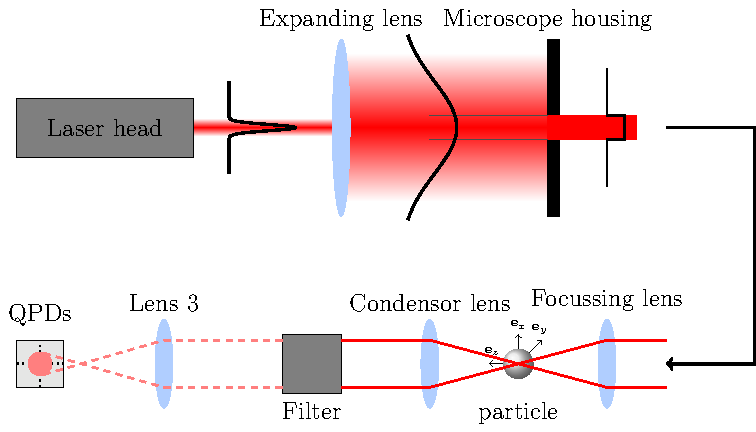
\includegraphics[]{Plots/cache/setup.pdf}
  \caption{Schematic of light path from laser head to quadrant photo detectors. 
  In the top half sketch red shading and the black lines the laser intensity 
profile qualitatively. In the bottom half just the outer most laser rays are 
depicted.}
  \label{fig:Th-setup}
\end{figure}

Before highlighting important parts from ray optics it is advantageous to 
understand our optical trapping setup which is based upon the work of Arthur 
Ashkin~\cite{Ashkin1978,Ashkin1987,Ashkin2002,Ashkin1986,Ashkin1992,Ashkin1997}. 
\cref{fig:Th-setup} depicts a basic schematic of the laser path from the laser 
source to the quadrant photo detectors (QPDs) in the back focal plane. A 
complete overview of our setup with a list and explanation of every used part 
is available in~\cite{Lamprecht2017}.

Our laser diode emits a tightly confined laser beam in the near-infrared regime 
(non-visible) with a wavelength of $\lal=\SI{785}{\nm}$ and a maximal power of 
$P=\SI{200}{\milli\watt}$ and with a transverse electromagnetic mode of order 
00 (TEM$_{00}$). This laser profile is axisymmetric to the light propagation 
direction and can be visualized with a rotating Gaussian bell curve. Next, the 
beam is expanded such that it is much larger than the opening of the microscope 
housing. The magnitude of the trapping forces are proportional to the laser 
intensity of the beam. The biggest contribution to the total force stems from 
the outer parts of the beam. Therefore, it is advantageous to broaden the beam 
before guiding it to the focusing lens. The opening of the microscope is 
overfilled by the broadened beam and the laser intensity after this cutoff can 
be approximated with a flat-top profile. Hence, every light wave (also the ones 
contributing most to the total trapping force) carries the same intensity.

The next step is the focusing of the beam with a high numerical aperture (NA) 
oil immersion lens. Here, the actual trapping of the particle occurs. If more 
than just the trapping of particles is of interest, the beam needs to be 
investigated further. The relative movement of the particle within the trap 
contains the necessary information. In order to image the movement in the $\ex$ 
and $\ey$ direction the beam is collimated again by the condensor lens after it 
passed the particle and filtered to reduce its total intensity to prevent 
damage of the QPDs. Before the beam is focussed, it is split into two because 
the axial movement detection for $\ez$ and the in plane movement detection for 
$\ex$ and $\ey$ have inherently different working principles.

If the particle moves within the trap the spot on the QPDxy will also move. By 
measuring the voltage on each quadrant of the QPDxy and summing and subtracting 
certain quadrants it is possible to retrieve the information about the movement 
in each direction separately. For the axial direction the opening of the QPDz 
is overfilled. An axial movement of the particle causes a change of total 
intensity on this QPD. By measuring the QPDz total intensity we have the 
information about the relative movement of the particle within the trap. After 
the calibration of the OT the measured voltages that are proportional to the 
particle movement can be converted to the physical unit meter. The calibration 
process itself is not relevant for this thesis but is available 
here~\cite{Lamprecht2017}. An discussion of different calibration options is 
available from \citeauthor{Svoboda1994}~\cite{Svoboda1994} and 
\citeauthor{Jun2004}~\cite{Jun2004}.


\textcolor{red}{which material parameters if fluid or water}

\section{Ray Optics\label{sec:Th-rayoptics}}

As said before, in the regime of ray optics the propagation of light is 
visualized by single rays. The interaction of a single ray at an interface is 
then studied geometrically. The defining property for these kind of 
investigations is the so called refractive index $\refraction$. Light travels 
in vacuum at speed of light $c=\SI{299792458}{\m\per\s}$. In other mediums than 
vacuum the speed of light has a different (smaller) magnitude. The refractive 
index relates the speed of light of vacuum $c$ to any other material $c_{\Box}$
\begin{equation}
  c_{\Box} = \frac{c}{n}.
  \label{eq:Th-lightspeed}
\end{equation}
Since there is nothing faster than the speed of light, the refractive index 
$\refraction$ cannot be smaller than 1. This index is not constant for one 
material but a function of the wavelength $\lambda$. Additionally, the 
refractive is in general a complex quantity
\begin{equation}
  \refraction\geq 1 \quad \wedge \quad \refraction \coloneqq 
  \refraction(\lambda) = \refraction(\lambda) - \iu k(\lambda)
  \label{eq:Th-refractive-index}
\end{equation}
where $k$ is called the extinction coefficient~\cite{Jackson2013}. 
\Cref{fig:Th-n_water} depicts $n$ and $k$ of water for different wavelengths 
$\lambda$. Whereas the real part of \cref{eq:Th-refractive-index} is about 
constant for $\lambda > \SI{400}{\nm}$, the complex part changes its magnitude 
over 4 orders of magnitude in the same interval.

\begin{figure}[tbp]
  \centering
  % \tikzsetnextfilename{n_water}
%%%%%%%
% READ TABLE
%%%%%%%

\begin{tikzpicture}
\begin{axis}[
  height=80mm,
  width=120mm,
  no markers,
  xlabel={$\lal$ [\si{\nm}]},
  ylabel={$\nreal$ [-]},
 ]

    \addplot[black] table[x=wl,y=n] 
    {\relPath/10_Figures/TikZ/Segelstein1981a.dat};

    \label{plot_n}
    \draw[dashed,<->,latex-latex] ({axis cs:785,0}|-{rel axis cs:0,0.0}) -- 
    (785,1.326244) -- node[above,pos=0.65,fill=white,opacity=0.8,text 
    opacity=1] {\footnotesize 1.326} ({0,1.326244}-|{rel axis cs:0,0});
\end{axis}
\begin{axis}[
  height=80mm,
  width=120mm,
  axis y line*=right,
  axis x line=none,
  ylabel={$\alpha$ [\si{\per\meter}]},
  no markers,
  ymode = log,
]
    \addlegendimage{/pgfplots/refstyle=plot_n}\addlegendentry{$\nreal$}
    \addplot[black,dash dot] table[x=wl,y=a] 
    {\relPath/10_Figures/TikZ/Segelstein1981a.dat};
    \addlegendentry{$\alpha$}

    \draw[dashed,<->,latex-latex] ({axis cs:785,0}|-{rel axis cs:0,0.0}) -- 
    (785,2.144) -- node[above,pos=0.73] {\footnotesize 2.144} 
    ({0,2.144}-|{rel axis cs:1,0});
    % 2.14353e+00

    \draw[dotted,<->,latex-latex] ({axis cs:1060,0}|-{rel axis cs:0,0.0}) -- 
    (1060,15.40) -- node[above,pos=0.53,fill=white,opacity=0.8,text 
    opacity=1] {\footnotesize 15.40} ({0,15.40}-|{rel axis cs:1,0});
    % 1.53991e+01
\end{axis}
\end{tikzpicture}

  \includegraphics[]{Plots/cache/n_water.eps}
  \caption{Index of refraction $n$ and extinction coefficient $k$ for water 
  over wavelength $\lambda$. Data taken from \cite{Hale1973,Segelstein1981}.}
  \label{fig:Th-n_water}
\end{figure}


The absorption coefficient~\cite{Hecht2017}
\begin{equation}
  \alpha = \frac{4\pi f k}{c} = \frac{4\pi}{\lambda}k
  \label{eq:Th-alpha}
\end{equation}
converts the dimensionless quantity $k$ into a physical parameter with unit 
\si{\per\meter}. Any ray of any wavelength is attenuated when propagating 
through a medium. The \emph{Beer-Lambert Law}
\begin{equation}
  \intensity(s) = \intensity_{0}\exp(-\alpha s)
  \label{eq:Th-beer-lambert}
\end{equation}
captures the change of intensity while moving along the path $s$ where 
$\intensity_{0}$ is the intensity at the start. E.g. in a depth of 
approximately \SI{1}{\kilo\meter} it is completely dark in the ocean because 
all the intensity of the sunlight is attenuated there.

\begin{figure}[tbp]
  \centering
  % \tikzsetnextfilename{Snell}

\tikzstyle arrowstyle=[scale=1]

\tikzstyle directed=[postaction={decorate,decoration={markings,
    mark=at position .65 with {\arrow[arrowstyle]{stealth}}}}]

\tikzstyle reverse directed=[postaction={decorate,decoration={markings,
    mark=at position .65 with {\arrowreversed[arrowstyle]{stealth};}}}]

\tikzset{SnellNode/.style={text width=10mm, align=center}}

\begin{tikzpicture}
  \def\W{5}
  \def\H{4}
  \def\x{0.95}
  \def\anglealpha{0}
  \pgfmathsetmacro{\y}{{(1-\x)*\H}}
  \pgfmathsetmacro{\radius}{(\W^2+\y^2)/2/\y}
  \pgfmathsetmacro{\anglealpha}{{asin(\W/\radius)}}
  \pgfmathsetmacro{\s}{{90+\anglealpha}}
  \pgfmathsetmacro{\e}{{90-\anglealpha}}

  \pgfmathsetmacro{\anglebeta}{{0.8*\anglealpha}}
  \pgfmathsetmacro{\p}{{(\radius-\H)*sin(\anglebeta)}}
  \pgfmathsetmacro{\px}{{\radius*sin(\anglebeta)}}
  \pgfmathsetmacro{\py}{{-\radius*(1-cos(\anglebeta))}}


  % define coordinates
  \coordinate (O) at (0,0) ;
  \coordinate (A) at (0,\H) ;
  \coordinate (B) at (0,-\H) ;

  % media
  \fill[blue!20,opacity=.3] (-\W,0) rectangle (\W,\H);
  \fill[black!10!,opacity=.3] (-\W,0) rectangle (\W,-\H);
  \node[right, SnellNode] at (2,1.5) {{Fluid\\ $\nf$}};
  \node[left, SnellNode] at (-2,-2) {{Particle\\ $\ns$}};

  % axis
  \draw[dash pattern=on5pt off3pt] (A) -- (B) ;
  % normal
  \draw[|->, thick] (0,0) -- node[right, pos=1] {$\normalvector$} (0, 2.5);


  % ray representation
  \def\gamma{130}
  \draw[red, variable=\x, domain=2.5:\W, samples=100] (0,\H) plot 
  ({\x*cos(\gamma)-cos(\x*pi r*3)/4*sin(\gamma)},{sin(\gamma)*\x+cos(\x*pi 
  r*3)/4*cos(\gamma)});

  % rays
  \draw[red,ultra thick,reverse directed] (O) -- node[left, xshift=-1mm, 
  pos=0.2] {$P_{\mathrm{i}}$} (130:5.2);

  \draw[red,ultra thick,directed] (O) -- node[right, xshift=1mm, pos=0.2] 
  {$P_{\mathrm{r}}$} (50:5.2);

  \draw[blue,directed,ultra thick] (O) -- node[right, xshift=1mm, pos=0.2] 
  {$P_{\mathrm{t}}$} (-70:4.24);

  % particle circumference
  \draw (-\W,-\y) arc (\s:\e:\radius);
  \draw[black,->|,>=stealth'] (\p,-\H) -- node[right, pos=0.7] {$\R$} (\px, 
  \py);

  % angles
  \draw[->,>=stealth'] (0,1) arc (90:130:1);
  \draw[->,>=stealth'] (0,1) arc (90:50:1);
  \draw[->,>=stealth'] (0,-1.4) arc (270:290:1.4);

  \node[] at (280:1.8)  {$\transmitted$};
  \node[] at (110:1.4)  {$\incident$};
  \node[] at (70:1.4)  {$\refracted$};

\end{tikzpicture}

  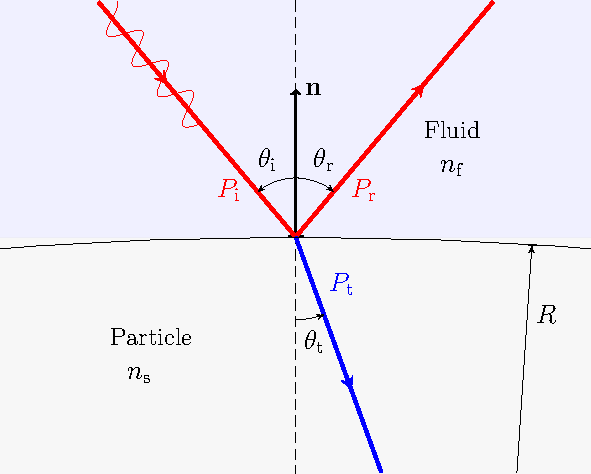
\includegraphics[]{Plots/cache/Snell.pdf}
  \caption{Visualization of \emph{Snell's Law} for rays at an interface of two 
  media with different refractive indices $\refraction_{\Box}$.}
  \label{fig:Th-Snell}
\end{figure}

With the real part of the complex refractive index, it is possible to define 
the most important relation in the ray optics regime. The \emph{Snell's Law} 
(see also \cref{fig:Th-Snell}) is defined as
\begin{equation}
  \nf\,\sin\incident = \ns\,\sin\transmitted.
  \label{eq:Th-Snell}
\end{equation}
It connects the angle of incident $\incident$ with the transmitted angle 
$\transmitted$ at an interface of two different media with refractive indices 
$\ns$ and $\nf$, respectively. This law is based on the fact that a ray of 
light travels on the fastest path (not the shortest) between two 
points~\cite{Born1980Ch3}. The angle of the reflected ray is equal to the 
incident angle ($\reflected=\incident$).

There is one more angle of special interest. It is the angle of total internal 
reflection $\theta_{\MR{TIR}}$
\begin{equation}
  \theta_{\MR{TIR}}=\incident \quad\forall\quad \frac{\nf}{\ns}\,\sin\incident 
  > 1.
  \label{eq:Th-TIR}
\end{equation}
For incident angles of this magnitude or greater 
($\incident\geq\theta_{\MR{TIR}}$), no ray is transmitted into the other 
medium. This can only occur if the index of refraction of the incident medium 
is greater than the transmitted medium ($\nf>\ns$ in \cref{fig:Th-Snell}) 
otherwise the ratio $\sfrac{\nf}{\ns}$ of \cref{eq:Th-TIR} is always smaller 
than unity and there is physically no total internal reflection possible.

% The other angle of special interest is the so called \emph{Brewster Angle} 
% $\theta_{\MR{B}}$
% \begin{equation}
  % \theta_{\MR{B}} = \tan^{-1}\left( \frac{\ns}{\nf} \right).
  % \label{eq:Th-brewster}
% \end{equation}
% At this angle there does not occur an reflection and hence all the intensity is 
% transmitted.

So far, \cref{eq:Th-Snell} calculates in which direction a ray will travel 
after an interface of two media. The amplitude of the reflected and transmitted 
rays can be computed with the so called \emph{Fresnel 
Equations}~\cite{Jackson2013,Born1980Ch1}. Although we think of light as rays, 
the theory behind those equations is based on the electromagnetic wave 
character of light. For time harmonic electromagnetic waves the amplitude of 
the incident electric wave vector $\vb{E}_{\MR{i}}$ to the transmitted 
$\vb{E}_{\MR{t}}$ and to the reflected $\vb{E}_{\MR{t}}$ electric wave vector 
is related by $\fresnelr_{i}$ and $\fresnelt_{i}$
\begin{subequations}
\begin{align}
  \vb{E}_{\MR{r}} & =\fresnelr_{i}\,\vb{E}_{\MR{i}} \\[3mm]
  \vb{E}_{\MR{t}} & =\fresnelt_{i}\,\vb{E}_{\MR{i}}
\end{align}
\end{subequations}
where the subscript $i$ can either be $i=\MR{p}$ for p-polarized light or 
$i=\MR{s}$ for s-polarized light~\cite{Jackson2013,Born1980Ch1}. ``s'' and 
``p'' stand for the German words ``parallel'' (parallel) and ``senkrecht'' 
(perpendicular), respectively. They refer to the to the orientation of the 
incident electric field $\vb{E}_{\MR{i}}$ to the plane of incident. For the 
special cases of ``p'' and ``s'' polarized light the Fresnel coefficient with 
the assumption that both media are non-magnetic ($\mu_{\MR{f}} = \mu_{\MR{s}} = 
\mu_{0} = 1$)~\cite{Born1980Ch1} are
\begin{subequations}
\begin{align}
  \fresnelr_{\MR{s}} & =
  \frac{2\,\nf\,\cos\incident}{\nf\,\cos\incident + \ns\,\cos\reflected} 
  \label{eq:Th-fresnel-rs}\\[3mm]
  \fresnelt_{\MR{s}} & = \frac{\nf\,\cos\incident - 
  \ns\,\cos\reflected}{\nf\,\cos\incident + \ns\,\cos\reflected} 
  \label{eq:Th-fresnel-ts}\\[3mm]
  \fresnelr_{\MR{p}} & =
  \frac{2\,\nf\,\cos\incident}{\ns\,\cos\incident + \nf\,\cos\reflected} 
  \label{eq:Th-fresnel-rp}\\[3mm]
  \fresnelt_{\MR{p}} & = \frac{\ns\,\cos\incident - 
  \nf\,\cos\reflected}{\ns\,\cos\incident + \nf\,\cos\reflected}.
\label{eq:Th-fresnel-tp}
\end{align}
\end{subequations}
So far, the Fresnel coefficients relate the amplitudes of the incident 
electrical field to the transmitted and reflected electrical field. In general, 
the sum of $\fresnelr$ and $\fresnelt$ does not add up to unity.

For \cref{sec:Th-temperature}, it is necessary to know how much of the incident 
power $P_{\MR{i}}$ is transmitted and how much is reflected. The power 
$P=\intensity A$ is a product of the intensity $\intensity$ and the area $A$ it 
is acting on. The intensity is defined as the timeaverage of the Ponyting 
vector $\vb{S}$
\begin{equation}
  \intensity = \timeaverage{\abs{\vb{S}}} = 
  \timeaverage{\abs{\vb{E}_{0}\times\vb{H}_{0}}} = 
  \frac{1}{2}\,\frac{\refraction}{Z_{0}}\,\abs{\vb{E}_{0}}^{2} = 
  \frac{1}{2}\,\refraction\,c\epsilon_{0}\,\abs{\vb{E}_{0}}^{2}
\end{equation}
where $Z_{0}$ is the electrical impedance of free space and $\epsilon_{0}$ is 
the vacuum permittivity. With 
\cref{eq:Th-fresnel-rs,eq:Th-fresnel-ts,eq:Th-fresnel-rp,eq:Th-fresnel-tp} the 
scaling of the electrical field at the interface is defined. With the relation 
(see also \cref{fig:Th-Snell})
\begin{equation}
  w = \frac{w_{\MR{i}}}{\cos\incident} = \frac{w_{\MR{r}}}{\cos\reflected} = 
  \frac{w_{\MR{t}}}{\cos\transmitted}
  \label{eq:Th-area}
\end{equation}
and the scaling of the power
\begin{equation}
  P = \intensity A \propto \refraction\,\abs{\vb{E}_{0}}^{2}A \propto
  \refraction\,\abs{\vb{E}_{0}}^{2}w
\end{equation}
one can calculate the reflectance $\fresnelR_{i}$ as the ratio of the reflected 
power $P_{\MR{r}}$ to the incident power $P_{\MR{i}}$ as
\begin{equation}
  \fresnelR_{i} = \frac{P_{\MR{r}}}{P_{\MR{i}}} = 
  \frac{\intensity_{\MR{r}}\,\nf\,w_{\MR{r}}}{\intensity_{\MR{i}}\,\nf\,w_{\MR{i}}} 
  =\frac{\abs{\fresnelr_{i}\,\vb{E}_{0}}^{2}}{\abs{\vb{E}_{0}}^{2}} = 
  \fresnelr_{i}^{2}
  \label{eq:Th-fresnelR}
\end{equation}
where again the italic $i$ in the subscript ($\Box_{i}$) is the polarization. 
Similarly one finds the transmittance $\fresnelT_{i}$ as
\begin{equation}
  \fresnelT_{i} = \frac{P_{\MR{t}}}{P_{\MR{i}}} = 
  \frac{\intensity_{\MR{t}}\,\ns\,w_{\MR{t}}}{\intensity_{\MR{i}}\,\nf\,w_{\MR{i}}} 
  =\frac{\abs{\fresnelt_{i}\,\vb{E}_{0}}^{2}}{\abs{\vb{E}_{0}}^{2}}\,\frac{\ns\,w_{\MR{t}}}{\nf\,w_{\MR{i}}} 
  = \fresnelt_{i}^{2}\,\frac{\ns\,\cos\transmitted}{\nf\,\cos\incident}.
  \label{eq:Th-fresnelT}
\end{equation}
For unploarized rays one can take the arithmetic average of $\Box_{\MR{s}}$ and 
$\Box_{\MR{p}}$ polarization values. Other than the Fresnel coefficients the 
sum of the reflectance $\fresnelR$ and the transmittance $\fresnelT$ for one 
angle of incidence need to be unity
\begin{equation}
  \fresnelR + \fresnelT = 
  \frac{\fresnelR_{\MR{s}}+\fresnelR_{\MR{p}}}{2} +
  \frac{\fresnelT_{\MR{s}}+\fresnelT_{\MR{p}}}{2} = 1 
  \label{eq:Th-fresnel}
\end{equation}
because the incident power $P_{\MR{i}}$ is either reflected or transmitted
\begin{equation}
  P_{\MR{i}} = P_{\MR{r}} + P_{\MR{t}} = P_{\MR{i}}\left( \fresnelR + \fresnelT 
  \right).
\end{equation}

\section{Laser Induced Temperature Change\label{sec:Th-temperature}}

A laser is a (highly focused) coherent beam of electromagnetic waves of a 
single wavelength $\lal$. Intensities with the orders of 
\si{\mega\watt\per\square\meter} and more are common. For comparison, the 
average intensity of the sun on to the earth in Central Europe is about 
\SI{1.36}{\kilo\watt\per\square\meter}, and the laser of our setup has with its 
peak power of \SI{200}{\milli\watt} and a specified beam diameter of 
\SI{1}{\mm} a maximal intensity of about 
\SI{0.25}{\mega\watt\per\square\meter}. As described with the Beer-Lambert-Law
(\cref{eq:Th-beer-lambert}) some of the laser intensity is attenuated while 
traveling through any medium. The attenuation of intensity will lead to an 
increase of temperature in the absorbing medium.

The intensity of a focused laser is highest in the region of the focal point 
because all its power is confined to a small area. Direct temperature 
measurements in the vicinity of the laser focus are due to the microscopic 
region of interest up to now not possible. Precise knowledge of the temperature 
change is of interest, e.g., for the calibration process of the OT but also for 
objects that need to stay below a certain temperature, e.g. living cells.

In the following, we will first discuss the current research regarding 
temperature increase in OTs, discuss the path of a ray through the particle, 
and then motivate a temperature approximation based on simple ray optics.

\subsection{State of the Art}\label{sec:Th-state}

\cyear{Liu1995} measured the temperature dependent change in fluorescence of 
biological cells while being trapped with a wavelength of 
$\lal=\SI{1064}{\nm}$. They found a linear relation between temperature 
increase and applied laser power of about \SI{15}{\degreeCelsius\per\watt}. In 
addition, they solved the heat problem also analytically. For that, they 
neglected the trapped object and modeled as water because their cells of 
interest consist mainly out of water. The experiments as well as the 
analytical solution show an almost instantaneous change in temperature after 
the laser is switched on. \cyear{Celliers2000} measured the local change in the 
index of refraction for water while being subjected to a laser with a 
wavelength of \SI{985}{\nm}. During the measurements no objects was trapped in 
the laser focus. They measured a temperature increase of \SI{4}{\degreeCelsius} 
with a laser power of \SI{55}{\milli\watt} in the focus of the laser. An 
analytical model that utilized an improved source term compared to 
\cite{Liu1995} validated their results.

\cyear{Peterman2003} measured with a OT of \SI{1064}{\nm} wavelength the 
effects of the temperature increase in the vicinity of the laser focus. A 
change of temperature in the fluid will lead to a change of the fluid 
viscosity. The viscosity change alters the calibration parameters of the OT. By 
fitting the calibration parameters for different laser powers to the 
theoretical relation they found a temperature increase of roughly 
\SI{8}{\degreeCelsius\per\watt} for water as fluid medium and silica beads as 
trapped object. More interestingly, their analytical model revealed that most 
of the heat absorption is in the fluid rather than the trapped object. In 
addition, usual glass coverslips act as fast heat conductor compared to water 
such that measurements close to the top or bottom surface of the fluid cavity 
lead to a minor temperature increase.

\cyear{Moreau2015} injected Rhodamine B (RhB) in cells to measure the 
temperature change of an OT with \SI{800}{\nm} wavelength. RhB is a temperature 
sensitive dye which changes its fluorescence linearly with the temperature. 
Since they injected the RhB into the cell the measured temperature difference 
was around the focal point. As before, the increase of the temperature occurs 
almost instantaneously and is about \SI{9}{\degreeCelsius\per\watt}. Lastly, in 
\citeyear{Catala2017}, \cname{Catala2017} studied the effects of different 
experimental parameters (numerical aperture (NA), material of trapped object, 
distance to coverslips, object radius) to the magnitude of the temperature 
increase with an OT of \SI{1064}{\nm} wavelength. A numerical model validated 
their experimental findings. Their source term which is an extension to 
\cname{Peterman2003} takes account of the NA, the finite focal spot size, and 
the wavelength of the laser itself. In agreement to the others they found the 
heat increase to be about \SI{20}{\degreeCelsius\per\watt}.

All of the aforementioned studies (see also \cref{tab:Th-heating}) validated in 
their experiments the linear relation of the applied laser power to the 
increase in temperature. Also, they showed that the temperature change occurs 
almost instantaneously and that a steady system is established in the range of 
\si{\ms}. In addition, they agree that the main absorption occurs in the fluid 
medium (water or glycerol) rather than the trapped object (polystyrene or 
silica) itself because the absorption coefficient $\alpha$ is greater. However, 
as can be seen in \cref{fig:Th-n_water}, the extinction coefficient is 
dependent on the wavelength $\lal$. Besides \cite{Moreau2015} all studies 
operate at a wavelength of \SI{1064}{\nm}. Our OT operates at \SI{785}{\nm} and 
the extinction coefficient $k$ for this wavelength is about one order of 
magnitude smaller than it is at \SI{1064}{\nm},
$k(\SI{785}{\nm}) \approx 1.339\cdot 10^{-7} \rightarrow \alpha(\SI{785}{\nm}) 
\approx \SI{2.14}{\per\meter} $ and $k(\SI{1064}{\nm}) \approx 1.299\cdot 
10^{-6} \rightarrow \alpha(\SI{1064}{\nm}) \approx \SI{15.4}{\per\meter} $ 
respectively. The magnitude of the absorption coefficient $\alpha$ is the 
measure for how much intensity gets absorbed. It contributes linear in the heat 
equation.

Besides the results of \cname{Peterman2003} the measured temperature increase 
is larger for the wavelength of \SI{1064}{\nm}. The magnitudes of the 
respective absorption coefficients $\alpha$ ($\sfrac{15.4}{2.14}\approx 7.2$) 
suggest a seven times greater heating for the larger wavelength. However, only 
the results of \cname{Celliers2000} compared to \cname{Moreau2015} match this 
interpolation. But they used an inherently different method for approximating 
the temperature increase where no object was trapped during the measurement. 
Despite having non-coherent results, we take a heating value of 
\SI{10}{\degreeCelsius\per\watt} for our wavelength of \SI{785}{\nm} as given 
for the following section if the focus of the OT is at least \SI{10}{\um} away 
from any surrounding surface.

\begin{table}
  \centering
  \begin{tabular}{l *{6}{c}}
    \toprule
    \toprule
    Author & $\lambda$ & Heating & Mat. & Exp.  & Ana. & Num. \\
    & [\si{\nm}] & [\si{\degreeCelsius\per\watt}] \\
    \midrule
    \cname{Liu1995} & 1064 & 15 & Cells & $\checkmark$ & $\checkmark$ & \\
    \cname{Celliers2000} & 985 & 72 & - & $\checkmark$ & $\checkmark$ & \\
    \cname{Peterman2003} & 1064 & 8 & Si & $\checkmark$ & $\checkmark$ & \\
    \cname{Moreau2015} & 800 & 9 & Cells & $\checkmark$ & & \\
    \cname{Catala2017} & 1064 & 20 & Si & $\checkmark$ & $\checkmark$ & $\checkmark$ \\
    \bottomrule
    \bottomrule
  \end{tabular}
  \caption{Overview of studies to laser induced heating in OTs. Mat.=Material 
  type of the trapped object, Ex.=Experimental part, Ana.=Analytical model, 
Num.=Numerical model}\label{tab:Th-heating}
\end{table}

\subsection[Ray Path \& absorbed Energy]{Ray Path through Particle and absorbed 
Energy}

Before approximating the heat distribution inside the trapped particle with ray 
optics, it is necessary investigate the path of the ray though the particle. In 
\cref{fig:Th-ray_particle} an ray with power $\power{i}{1}$ is incident on the 
particle surface in point $I$. The direction of the ray is towards the focal 
point $f$ which is slightly above the middle point $M$ of the particle because 
the stable trapping position is the equilibrium of the trapping forces towards 
the point $f$ and gravity. Because of the different refractive indices of the 
fluid $\nf$ and the particle $\ns$ the ray gets deflected inside the particle. 
The transmitted angle $\transmitted$ can easily be computed with 
\cref{eq:Th-Snell}. However, for that the incident angle $\incident$ must be 
known.

\begin{figure}[thp]
  \centering
  % \tikzsetnextfilename{ray}
{
\small

\tikzset{cross/.style={
  cross out,
  draw=black,
  minimum size=2*(#1-\pgflinewidth),
  inner sep=0pt, outer sep=0pt},
  cross/.default={1pt}}

\tikzstyle arrowstyle=[scale=2]

\tikzstyle directed=[postaction={decorate,decoration={markings,
    mark=at position .5 with {\arrow[arrowstyle]{stealth}}}}]

\tikzstyle reverse directed=[postaction={decorate,decoration={markings,
    mark=at position .65 with {\arrowreversed[arrowstyle]{stealth};}}}]

\begin{tikzpicture}[scale=1.5]

  % define coordinates
  \coordinate (O) at (0,0) ;
  \coordinate (F) at (0,0.15) ;
  \coordinate (N) at (260:2) ;

  % medium
  \filldraw[blue!20!, opacity=0.3] (-3,-3) rectangle ++(6,6);


  % particle
  \draw[fill=white] (O) circle (2);
  \draw[fill=black!10!, opacity=0.3] (O) circle (2);

  \node[circle, fill=black, inner sep=0pt, minimum size=3pt, label=left:{$M$}] 
  at (O) {};
  \node[circle, fill=black, inner sep=0pt, minimum size=3pt, label=above:{$f$}] 
  at (F) {};

  % rays
  \coordinate (I) at (28.6:2) ;
  \node[circle,fill=black,inner sep=0pt,minimum size=3pt,label=above:{$I$}] at 
  (I) {};
  \node[circle,fill=black,inner sep=0pt,minimum size=3pt,label=right:{$N$}] at 
  (N) {};
  \draw[directed,red] (2.5,1.3) -- node[below, midway] {$\power{i}{1}$} (I);
  \draw[directed,red] (N) -- node[left,xshift=-0.1mm] {$\power{t}{2}$} 
  (258:2.8);

  \draw[directed, blue] (I) -- node[right,midway,xshift=0.1mm] 
  {$\power{t}{1}=\power{i}{2}$} (N);

  \draw[directed, blue] (N) -- node[left,midway,xshift=-0.1mm] 
  {$\power{r}{2}=\power{i}{3}$} (131.4:2);

  % arcs
  \draw[<-,>=stealth'] ([shift=(234:0.5)]I) arc (234:209:0.5);

  \draw[<->,>=stealth'] ([shift=(55:0.5)]N) arc (55:105:0.5);

  \node[] at (22:1.2) {$\transmitted^{1}$};
  \node[] at (269:1.2) {$\incident^{2}$};
  \node[] at (254:1.22) {$\reflected^{2}$};

  % middle to hitting point
  \draw[densely dotted] (O) -- node[below,pos=0.3] {$\R$} (I);
  \draw[densely dotted] (O) -- node[left,pos=0.3] {$\R$} (N);
  \draw[red, dotted] (I) -- (F);
  % surface normal
  \draw[|->,>=stealth'] (N) -- node[right,pos=0.9] {$\normalvector$} (260:3);
  \draw[|->,>=stealth'] (I) --node[above,pos=0.9] {$\normalvector$} (28.6:3);

  % text
  \node[align=center, text width=15mm] at (-0.5,1) {{particle\\ $\ns$}};
  \node[align=center, text width=15mm] at (1.5,2) {{fluid\\ $\nf$}};

\end{tikzpicture}
}

  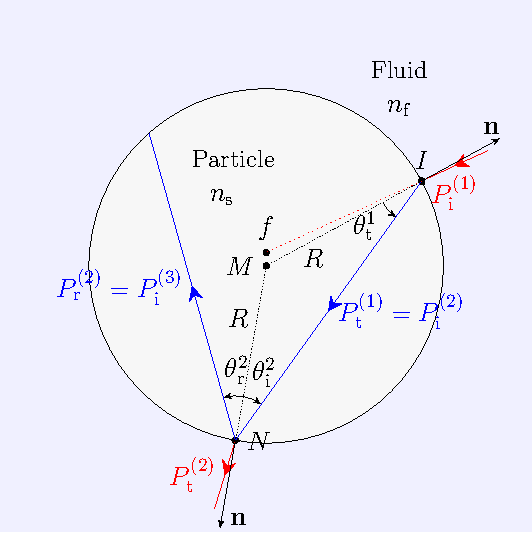
\includegraphics[]{Plots/cache/ray.pdf}
  \caption{Schematic of ray path through particle.}
  \label{fig:Th-ray_particle}
\end{figure}

With the convergence angle $\beta$ (see \cref{fig:Th-angles}) and the sine-law
\begin{equation}
  \frac{\sin\left( \frac{\pi}{2}-\beta \right)}{\R} = 
  \frac{\sin\incident}{a\,\R}
  \label{eq:Th-sine-law}
\end{equation}
one can compute $\incident$ as function of $\beta$. The angle $\beta$ is an 
input parameter and therefore known. The maximal convergence angle 
$\beta_{\MR{max}}$ is evaluated by the definition of the NA
\begin{equation}
  \text{NA} = \nf\,\sin\beta_{\MR{max}}.
  \label{eq:Th-NA}
\end{equation}
Our lens has a NA of 1.27 and water has a refractive index of $\nf=1.33$ (see 
\cref{fig:Th-n_water}) and therefore is our maximal convergence angle 
$\beta_{\MR{max}} \approx \SI{72}{\degree}$.

With the knowledge of $\transmitted^{1}$ the path of the ray inside the 
particle is determined. At the next intersection point of the ray with the 
particle surface $N$, the ray is again partly transmitted into the fluid and 
partly reflected. Since the triangle $\bigtriangleup_{IMN}$ is an isosceles 
triangle (two sides have the same length; here $R$) and per definition the 
reflected angle equals the incident angle, all internal reflection angles for 
one ray have the same magnitude 
($\transmitted^{1}=\incident^{n}=\reflected^{n}$ for $n>1$).

Now, the respective powers of one ray can be evaluated. The ray has the 
incident power $\power{i}{1}$ with every reflection it gets split into two 
portions. With \cref{eq:Th-fresnelR,eq:Th-fresnelT,eq:Th-fresnel} the powers 
after each reflection is
\begin{subequations}
  \begin{alignat}{3}
    \power{t}{1} & = \fresnelT\left( \incident^{1} \right)\,\power{i}{1} && \\
    \power{r}{2} & = \fresnelR\left( \transmitted^{1} \right)\,\power{t}{1} && 
    = \power{i}{1}\,\fresnelT\left( \incident^{1} \right)\,
    \fresnelR\left( \transmitted^{1} \right) \\
    \power{t}{2} & = \fresnelT\left( \transmitted^{1} \right)\,\power{t}{1} && 
    = \power{i}{1}\,\fresnelT\left( \incident^{1} \right)\,
    \fresnelT\left( \transmitted^{1} \right) \\
    \power{r}{3} & = \fresnelR\left( \transmitted^{1} \right)\,\power{i}{3} && 
    = \power{i}{1}\,\fresnelT\left( \incident^{1} \right)\,
    \fresnelR^{2}\left( \transmitted^{1} \right).
\end{alignat}
\end{subequations}

\begin{figure}[thp]
  \centering
  % \tikzsetnextfilename{angles}

\tikzstyle arrowstyle=[scale=2]
\tikzstyle directed=[postaction={decorate,decoration={markings,
    mark=at position .65 with {\arrow[arrowstyle]{stealth}}}}]

\begin{tikzpicture}[scale=1.3]
    \coordinate (O) at (0,0);
    \coordinate (I) at (4,3);
    \coordinate (A) at (0,1.4);

    \node[circle,fill=black,inner sep=0pt,minimum size=3pt,label=below:{$M$}] 
    at (O) {};
    \node[circle,fill=black,inner sep=0pt,minimum size=3pt,label=left:{$f$}] at 
    (A) {};
    \node[circle,fill=black,inner sep=0pt,minimum size=3pt,label=above:{$I$}] 
    at (I) {};

    % \draw (O) -- node[midway, below, xshift=1mm] {$R$} (I) -- node[above, 
    % midway, xshift=-1mm] {$y$} (A) -- node[midway, left] {$a\,R$} cycle;
    \draw (O) -- node[midway, below, xshift=1mm] {$\R$} (I) -- (A) -- 
    node[midway, left] {$a\,\R$} cycle;

    % \draw[dotted] (O) rectangle (I);
    \draw[dotted] (A) -- ++(0,1);

    \draw[->,>=stealth'] (I) -- node[above,midway] {$\normalvector$} (36.86:6);

    \draw[directed,red] (34.0:6.2) -- (I);


    \draw[] (0,0.5) arc (90:37:0.5) node[midway, above] {$\gamma$};
    \draw[] (0,1.9) arc (90:22:0.5) node[midway, above] {$\beta$};
    \draw[] (0,1.1) arc (-90:22:0.3) node[midway, right] 
    {$\sfrac{\pi}{2}-\beta$};
    \draw[] (36.8:3.5) arc (216:200.5:1.5) node[pos=.3, left] {$\incident$};

    \draw[] (I) arc (36.86:48:5);
    \draw[] (I) arc (36.86:-3:5);

\end{tikzpicture}

  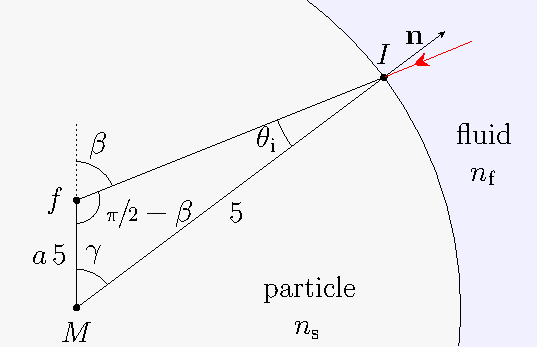
\includegraphics[]{Plots/cache/angles.pdf}
  \caption{Sketch of incident ray onto particle surface.}
  \label{fig:Th-angles}
\end{figure}

If a particle is stably trapped the distance $a$ of the particle center point 
$M$ and the focal point $f$ (see also \cref{fig:Th-angles}) is about $a \approx 
0.1\,R$~\cite{Lamprecht2017}. During the trapping process and due to external 
forces this distances changes. If the focal point is outside the particle, the 
trapping forces are negligible small.

\cref{fig:Th-gamma_theta} depicts the values of $\gamma$ and $\incident$, 
respectively, for different combinations of $a$ and $\beta$. As pointed out 
before, the distance $a$ is about $0.1\,R$. For this value the maximal incident 
angle $\incident$ over the whole range of $\beta$ is less than 
\SI{10}{\degree}.

\begin{figure}
  \centering
  \begin{subfigure}[b]{0.45\textwidth}
    \centering
    % \tikzsetnextfilename{gamma}
%%%%%%%
% READ TABLE
%%%%%%%

\begin{tikzpicture}
    \begin{axis}[view={0}{90},
        xlabel={$a$ [-]},
        ylabel={$\beta$ [\si{\degree}]},
        xmax=0.5,
        height=60mm,
        point meta min=0,
        point meta max=72,
        width=60mm,
        colormap/YlGnBu-9,
        colorbar,
        colorbar horizontal,
        colorbar style={
          title={$\gamma$ [\si{\degree}]},
          at={(0,1.3)},
          anchor=north west,
          xtick={0,24,48,72},
        },
        ytick={0,24,48,72},
        xtick={0,0.25,0.5},
      ]
      % countourf
      \addplot3[surf,mesh/rows=51,shader=interp] table[x=a,y=beta,z=gamma] 
      {\relPath/10_Figures/TikZ/angles_mat.dat};
      % lines
       \addplot3[
         mesh/rows=51,
         mesh/cols=50,
         contour gnuplot={levels={9,18,36,54},draw color=black},
     ] table[x=a,y=beta,z=gamma] {\relPath/10_Figures/TikZ/angles_mat.dat};

    \end{axis}
\end{tikzpicture}

    \caption{}
    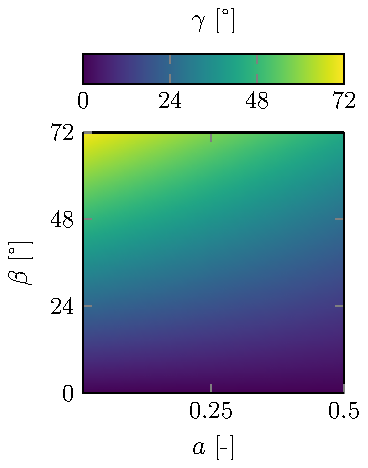
\includegraphics[]{Plots/cache/gamma.pdf}
    \label{fig:Th-gamma}
  \end{subfigure}
  \hfill
  \begin{subfigure}[b]{0.45\textwidth}
    \centering
    % \tikzsetnextfilename{theta_i}
%%%%%%%
% READ TABLE
%%%%%%%

\begin{tikzpicture}
    \begin{axis}[view={0}{90},
        xlabel={$a$ [-]},
        ylabel={$\beta$ [\si{\degree}]},
        xmax=0.5,
        height=60mm,
        point meta min=0,
        point meta max=30,
        width=60mm,
        colormap name=viridis,
        colorbar,
        colorbar horizontal,
        colorbar style={
          title={$\incident$ [\si{\degree}]},
          at={(0,1.3)},
          anchor=north west,
          xtick={0,10,20,30},
        },
        ytick={0,24,48,72},
        xtick={0,0.25,0.5},
      ]
      \addplot3[surf,mesh/rows=51,shader=interp] table[x=a,y=beta,z=theta] 
      {\relPath/10_Figures/TikZ/angles_mat.dat};
    \end{axis}
\end{tikzpicture}

    \caption{}
    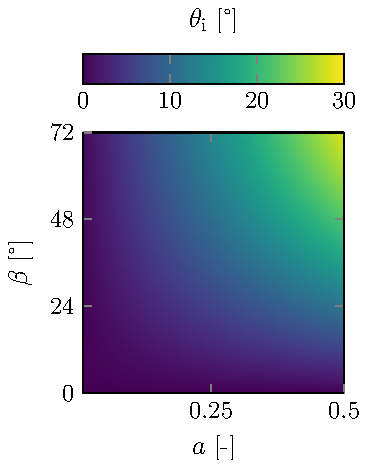
\includegraphics[]{Plots/cache/theta_i.pdf}
    \label{fig:Th-theta_i}
  \end{subfigure}
    \caption{Magnitude of $\gamma$ and $\incident$ for different values of $a$ 
    and $\beta$ (see also \cref{fig:Th-angles}).}
  \label{fig:Th-gamma_theta}
\end{figure}

\begin{figure}[tbp]
  \centering
  % \tikzsetnextfilename{Fresnel}
%%%%%%%
% READ TABLE
%%%%%%%
\pgfplotstableread{\relPath/10_Figures/TikZ/Fresnel.dat}{\data}

\begin{tikzpicture}
  \begin{groupplot}[
    axis on top=true,
    group style={
      group size=2 by 1,
      horizontal sep = 23mm,
    },
    xmin=0,
    ymin=0,
    height=55mm,
    width=73mm,
    no markers,
  ]
  \nextgroupplot[
    xlabel={Incident angle $\incident$ [\si{\degree}]},
    ylabel={\footnotesize Fresnel Coefficient [-]},
    xtick={0,0.16666,0.333333,0.5},
    xticklabels={0, 30, 60, 90},
    legend style={
      at={(axis cs:0.01,0.5)},
      anchor=west,
      font=\footnotesize,
    }
  ]
  \filldraw[black!10!,opacity=0.7] (0.155,0) rectangle ({0.5,1}|-{rel axis 
  cs:1,1});

    \addplot[dashed] table[x=theta,y=R_M2P] {\data};
    \addlegendentry{$\fresnelR_{\mathrm{f\rightarrow s}}$};
    \addplot[] table[x=theta,y=T_M2P] {\data};
    \addlegendentry{$\fresnelT_{\mathrm{f\rightarrow s}}$};

    \addplot[thick, blue, dotted] table[x=theta,y=R_P2M] {\data};
    \addlegendentry{$\fresnelR_{\mathrm{s\rightarrow f}}$};
    \addplot[thick, blue] table[x=theta,y=T_P2M] {\data};
    \addlegendentry{$\fresnelT_{\mathrm{s\rightarrow f}}$};

    \nextgroupplot[
    xlabel={Incident angle $\incident$ [\si{\degree}]},
    xmax=0.167,
    ymin=0.001,
    ymode=log,
    xtick={0,0.05555,0.11111,0.1666666},
    xticklabels={0, 10, 20, 30},
  ]

  \filldraw[black!10!,opacity=0.7] (0.155,0.00001) rectangle ({0.167,1}|-{rel 
  axis cs:1,1});

    \addplot[dashed] table[x=theta,y=R_M2P] {\data};
    \addplot[] table[x=theta,y=T_M2P] {\data};

    \addplot[thick, blue, dotted] table[x=theta,y=R_P2M] {\data};
    \addplot[thick, blue] table[x=theta,y=T_P2M] {\data};

  \end{groupplot}
  % \draw[thick,blue,->,shorten >=2pt,shorten <=2pt] (group c1r1.east) -- (group 
  % c2r1.west);
\end{tikzpicture}

  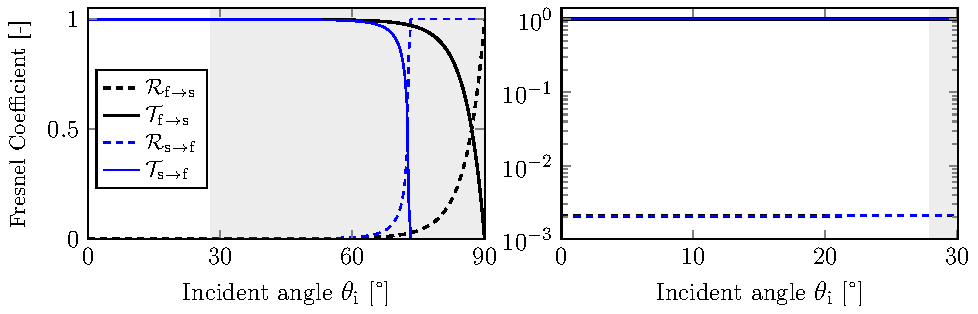
\includegraphics[]{Plots/cache/Fresnel.pdf}
  \caption{Fresnel coefficients of reflectance and transmittance (see 
  \cref{eq:Th-fresnelR,eq:Th-fresnelT}) for a water-particle interface 
  ($\Box_{\MR{f}\rightarrow\MR{s}}$) and a particle-water interface 
($\Box_{\MR{s}\rightarrow\MR{f}}$). The right plot is a detail of the left one 
with a logarithmic y-scale. The grey shaded area marks the interval of incident 
angles $\incident$ that do not occur in our setup.}
  \label{fig:Th-fresnel}
\end{figure}

Finally all is in place, to estimate the total relative absorbed energy 
$\delta$ by the particle.  \cref{eq:Th-intensity} defines the intensity after 
the distance $s$. Hence the relative absorbed energy over this length is
\begin{equation}
    \intensity_{\MR{abs}} = \intensity_{0} \left( 1 - \exp(-\alpha\,s) \right).
    \label{eq:Th-absorbed_energy}
\end{equation}
The distance $s$ for one passage through the particle can be computed as 
function of $\beta$ as
\begin{equation}
  s\left( \beta \right) = 2\,R\,\cos\left( \transmitted\left[ \incident\left( 
    \beta \right) \right]
    \right).
    \label{eq:Th-distance_s}
\end{equation}
And the power of a ray after $j$ reflections is
\begin{equation}
  \power{j}{i} =
  \fresnelT_{\MR{f}\rightarrow\MR{s}}\left( \incident \right) \,
  \fresnelR^{(j-1)}_{\MR{s}\rightarrow\MR{f}}\left( \transmitted \right)
  \label{eq:Th-power}
\end{equation}
With \cref{eq:Th-absorbed_energy,eq:Th-distance_s,eq:Th-power} the relative 
absorbed energy $\delta$ inside the particle can be approximated with discrete 
values
\begin{equation}
  \beta_{n} = \frac{n}{N}\,\beta_{\MR{max}}.
  \label{eq:Th-beta-disc}
\end{equation}
to be
\begin{equation}
  \intensity_{\MR{tot.,abs.}} \approx
  \frac{2\pi}{N}
  \sum\limits_{n=1}^{N}
  \sum\limits_{k=0}^{\infty}\power{i}{k-1}\left( \beta_{n} \right)\left[ 1 - 
  \exp\left( -\alpha\,s\left( \beta_{n} \right) \right) \right]
  \label{eq:Th-total-absorbed}
\end{equation}
where the factor $\sfrac{1}{N}$ is due to the assumption that each ray has the 
same incident power when hitting the particle surface and the factor $2\pi$ for 
considering the full volume of the particle. Per definition is the reflectance 
$\fresnelR$ or the transmittance $\fresnelT$ smaller than 1. This property as 
well as
\begin{equation}
  \sum\limits^{\infty}_{k=0} \Box^{k} = \frac{1}{1-\Box}
  \quad\text{for}\quad\abs{\Box} < 1
\end{equation}
can be applied to \cref{eq:Th-total-absorbed} to simplify the double sum to
\begin{equation}
  \intensity_{\MR{tot.,abs.}} \approx
  \frac{2\pi}{N}
  \sum\limits_{n=1}^{N}
  \fresnelT_{\MR{f}\rightarrow\MR{s}}\left( \incident \right)
  \left[ 1 - \exp\left( -\alpha\,s\left( \beta_{n} \right) \right) \right]
\,\frac{1}{1-\fresnelR_{\MR{s}\rightarrow\MR{f}}\left( \transmitted \right)}
  \label{eq:Th-total-absorbed-simp}
\end{equation}
where $\incident$ and $\transmitted$ are also function of $\beta_{n}$.

\cref{fig:Th-fresnel} depicts the values for $\fresnelT$ and $\fresnelR$ for 
the fluid-particle interface and the particle-fluid interface. Noteworthy is 
the fact, that for the occurring incident angles $\incident \leq 
\SI{10}{\degree}$ the values of $\fresnelR$ for both interface are less than 
$3\cdot 10^{-3}$. Therefore, most of the energy is transmitted and almost none 
reflected. For example, the relative power after one internal reflection and 
for an incident angle of $\incident=\SI{10}{\degree}$ is $\approx 2.07\cdot 
10^{-3}\,\power{i}{1}$ and after two internal reflections already $\approx 
4.31\cdot 10^{-6}\,\power{i}{1}$.

\begin{figure}[tbp]
  \centering
  % \tikzsetnextfilename{absorbed_energies}

\begin{tikzpicture}
  \begin{axis}[
      view={0}{90},
      ylabel={$\nicefrac{\Rprime}{\R}$ [-]},
      xlabel={$R$ [\si{\um}]},
      height=50mm,
      width=100mm,
      point meta min=0.2,
      point meta max=2.7,
      colorbar,
      colormap/BuPu-9,
      colorbar horizontal,
      colorbar style={
        title={\footnotesize Relative absorbed Energy $\Xi$ ($\times 
        10^{-4}$)},
        at={(0,1.4)},
        anchor=north west,
        xtick={0.2,0.5,1.0,1.5,2.0,2.5},
      },
    ]
      % contourf
      \addplot3[surf,mesh/rows=21,shader=interp] table[x=R,y=a,z=alpha] 
      {\relPath/10_Figures/TikZ/absorbed_energies.dat};
      % lines
       \addplot3[
         mesh/rows=21,
         mesh/cols=20,
         contour gnuplot={draw color=black},
     ] table[x=R,y=a,z=alpha] {\relPath/10_Figures/TikZ/absorbed_energies.dat};

  \end{axis}
\end{tikzpicture}

  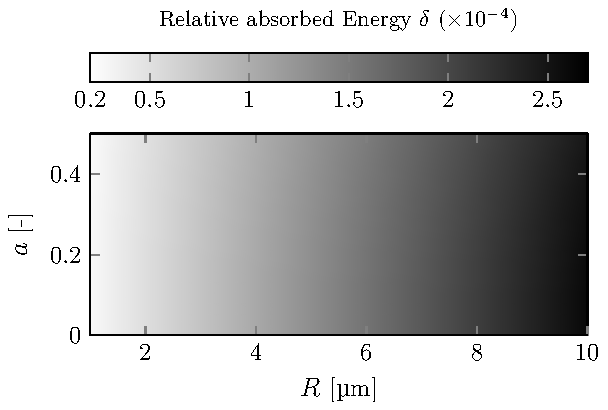
\includegraphics[]{Plots/cache/absorbed_energies.pdf}
  \caption{Results of \cref{eq:Th-total-absorbed-simp} for various relative 
  distances $a$ and radii $R$ with $N=500$ }
  \label{fig:Th-absorbed_energies}
\end{figure}

\cref{fig:Th-absorbed_energies} shows the relative absorbed energy $\delta$ 
inside a particle for various radii $R$ and distances $a\,R$. As 
\cref{fig:Th-fresnel} already suggested only a little fraction of the trapping 
energy is absorbed by the particle itself.

\subsection{Ray Optics Heat Approximation}

\begin{figure}[tbp]
  \centering
  % \tikzsetnextfilename{coordinate}

\begin{tikzpicture}[line cap=round, line join=round, >=Triangle, scale=1.5]

\clip(-2.1,-2.1) rectangle (2.38,2.58);
\filldraw[blue!20,opacity=.3] (-2.1,-2.1) rectangle (2.38,2.58);
\filldraw[white] (0,0) circle (2cm);

\draw[ball color=gray!20!white, fill opacity=0.6] (0,0) circle (2cm);

\draw [rotate around={0.:(0.,0.)},dash pattern=on 3pt off 3pt] (0,0) ellipse 
(2cm and 0.9cm);

\draw (0,0) -- (0.70,1.07) node[right, pos=0.4] {$r$};


\draw[-latex,line width=0.7pt]   (0,0) -- +(0,2) node[above] {$\ez$};
\draw[-latex,line width=0.7pt]   (0,0) -- +(-0.83,-0.81) node [left, 
yshift=-1.8mm] {$\ex$};
\draw[-latex,line width=0.7pt]  (0,0) -- +(2,0) node [right] {$\ey$};


\draw [-Latex, <-, >=stealth', shift={(0,0)}, black, fill opacity=1] (56.7:0.4) 
arc (56.7:90.:0.4) node[above, pos=0.3] {$\theta$};

\begin{scope}[rotate around x=10, y=10, xshift=1, yshift=-4.6]
    \draw [-Latex, ->, >=stealth', shift={(0,0)}, black, fill opacity=1] 
    (-135.7:0.4) arc (-135.7:-33.2:0.4) node[below,pos=0.4] {$\varphi$};
\end{scope}

\draw [dotted] (0.7,1)-- (0.7,-0.46);
\draw [dotted] (0,0)-- (0.7,-0.46);
\draw [fill] (0,0) circle (1.5pt);
\draw [fill] (0.7,1.07) circle (0.5pt);
\end{tikzpicture}

  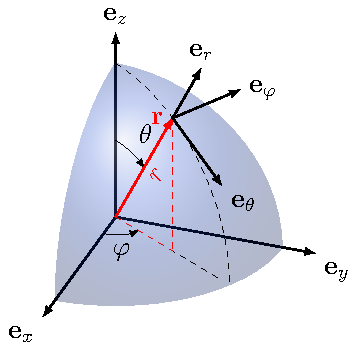
\includegraphics[]{Plots/cache/coordinate.pdf}
  \caption{Sketch of Cartesian and spherical coordinate system}
  \label{fig:Th-coordinate}
\end{figure}

With the knowledge of the relative absorbed energy $\delta$ of the particle, we 
solve the state heat equation for the particle
\begin{equation}
  \laplacian{T} = \frac{1}{\kappa} \pdv{T}{t} - \frac{q}{K}
  \label{eq:Th-heat-prob}
\end{equation}
where $T$ is the temperature inside the particle, $q$ is the absorbed energy of 
unit volume, $K$ the thermal conductivity, and $\kappa$ the thermal 
diffusivity. Further, we neglect the time-dependence $\pdv{T}{t}= 0$
\begin{equation}
  \laplacian{T} = - \frac{q}{K}
  \label{eq:Th-heat-stat}
\end{equation}
because all publications presented in \cref{sec:Th-state} state that the 
heating occurs within \si{\ms} and is negligible afterwards. In addition, we 
assume a spherical particle and solve the problem with spherical coordinate 
system (see \cref{fig:Th-coordinate}) with its origin at the particle center. 
Furthermore, we take the source term $q$ to be constant throughout the 
particle. Therefore, we neglect all partial derivatives to the angles $\varphi$ 
and $\theta$ and solve an ordinary differential equation
\begin{equation}
    \frac{1}{r^{2}}\pdv{r}\left( r^{2}\pdv{T}{r} \right) = - \frac{q}{K}
  \label{eq:Th-heat-spherical}
\end{equation}
with only a $r$ dependence and constant source term. We complete the problem, 
with two boundary conditions
\begin{subequations}
\begin{align}
  \eval{\pdv{T}{r}}_{r=0} &= 0\\[3mm]
  \eval{T}_{r=R_{0}} &= T_{0}.
\end{align}
\end{subequations}
The first one implies a bounded temperature at the origin ($r=0$) and the 
second one fixes the temperature at the surface of the particle ($r=R_{0}$). 
After two consecutive integration and applying of the boundary conditions one 
finds the difference temperature to be
\begin{equation}
  \Delta T(r) = T(r) - T_{0} = \frac{q}{6K}\left( R_0^2 - r^{2} \right).
  \label{eq:Th-heat-sol}
\end{equation}
The average temperature over the whole particle is the volume integral of 
\cref{eq:Th-heat-sol}
\begin{equation}
  \overline{\Delta T} = \frac{1}{V}\int_{V}\Delta T(r) \dd{V} = 
  \frac{1}{15}\,\frac{q}{K}\,R^{2}_{0}.
  \label{eq:Th-heat-avg}
\end{equation}
This can be further simplified since $q$ is the absorbed energy per unit volume
\begin{equation}
  q = \frac{\delta\,P}{V} = \frac{3\delta\,P}{4\,\pi\,R_{0}^{3}}
\end{equation}
where $P$ is the power of the laser and $\delta$ the relative absorbed energy 
of the particle. Finally, the average temperature increase of the spherical 
particle is
\begin{equation}
  \overline{\Delta T} = \frac{1}{20\,\pi}\,\frac{\delta\,P}{R_{0}\,K}.
  \label{eq:Th-heat-sol-simp}
\end{equation}
Interestingly, \cref{eq:Th-heat-sol-simp} seems to scale with $\propto 
\sfrac{1}{R_{0}}$. However, the relative total absorbed energy $\delta$ is also 
dependent on $R_{0}$ because the distance $s$ increases with the particle size 
linearly. But $\delta$ scales with $\left[  1-\exp\left( -\alpha\,R_{0} 
\right)\right]$ and therefore the average difference temperature 
$\overline{\Delta T}$ is proportional to $\sfrac{\left[ 1-\exp\left( 
-\alpha\,R_{0} \right) \right]}{R_{0}}$. This seems counter-intuitive, that 
bigger particle sizes lead to less temperature increase. But this only holds 
for the average temperature difference $\overline{\Delta T}$, the temperature 
distribution $T(r)$ (\cref{eq:Th-heat-sol}) increases with the particle size.

\begin{figure}[tbp]
  \centering
  % \tikzsetnextfilename{dT}
%%%%%%%
% READ TABLE
%%%%%%%
\begin{tikzpicture}
    \begin{axis}[view={0}{90},
        xlabel={$R$ [\si{\um}]},
        ylabel={$P$ [\si{\milli\watt}]},
        height=60mm,
        width=100mm,
        point meta min=0,
        point meta max=70,
        colormap = {whitered}{
          color(0cm) = (white);
          color(1cm) = (red)},
        colorbar,
        colorbar style={
          ytick={0,35,70},
          ylabel={$\overline{\Delta T}$ [\si{\milli\degreeCelsius}]},
        },
        xtick={1,5,10},
      ]
      % contourf
      \addplot3[
        surf,
        mesh/rows=21,
        shader=interp
      ] table[x=R,y=P,z=dT] {\relPath/10_Figures/TikZ/dT.dat};
      % lines
       \addplot3[
         mesh/rows=21,
         mesh/cols=20,
         contour gnuplot={levels={15,30,45,60},draw color=black},
     ] table[x=R,y=P,z=dT] {\relPath/10_Figures/TikZ/dT.dat};
    \end{axis}
\end{tikzpicture}

  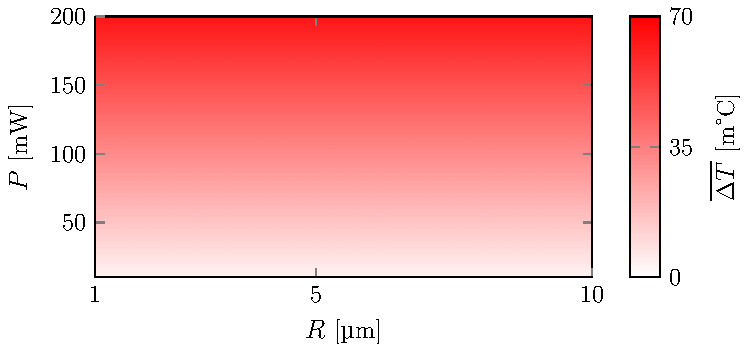
\includegraphics[]{Plots/cache/dT.pdf}
  \caption{$\overline{\Delta T}$ of \cref{eq:Th-heat-sol-simp} for various 
  laser powers $P$ and particle radii $R$.}
  \label{fig:Th-dT}
\end{figure}

\Cref{fig:Th-dT} depicts the average difference temperature for various 
combinations of laser power $P$ and particle radius $R$. With the information 
given in the aforementioned experimental studies regarding the heating by the 
laser and these ray optics motivated results for the heat distribution inside 
the particle, we conclude that the increase in temperature around and inside 
the particle for our setup is less than \SI{2}{\degreeCelsius} with the laser 
power in the low \si{\milli\watt} range we are applying.

Having established an upper bound for the laser induced temperature increase, 
we can estimate the effects of this increase to the absolute value of a 
measured force with the OT. The parameter that changes the most with a change 
in the temperature is the dynamic viscosity $\muef$ of the fluid. The viscosity 
is in general a function of the temperature $\muef\coloneqq\muef(T)$. For our 
calibration routine the absolute measured force of the OT scales with square 
root of the fluid viscosity ($\abs{\vb{\force}}\propto\sqrt{\muef}$). For the 
range of \SIrange{20}{30}{\degreeCelsius} the dynamic viscosity of water (exact 
formula from \cite{Peterman2003}) can be linearly approximated with
\begin{equation}
  \muef(T) = 8.9086\cdot 10^{-4} -2.0277\cdot10^{-5} (T-25).
  \label{eq:Th-viscosity}
\end{equation}
Temperature deviations of $\SI{25}{\degreeCelsius}\pm\SI{2}{\degreeCelsius}$ 
lead to force magnitude errors of less than $\pm$2.5\%.

\section{Optical Position Detection\label{sec:Th-QPD}}

Besides trapping the OT can also measure the relative movement of the trapped 
object within the trap. After a calibration it is also possible to convert the 
movement into the physical unit of meters and then also convert it into a force 
with unit Newton. Besides doing the movement tracking visually with, e.g., a 
high-speed camera, the most common approach is do utilize quadrant photo diodes 
(QPDs). The latter is superior to the camera because higher sampling 
frequencies are straightforward achievable, less data is produced during the 
measurement, as well as, a full three dimensional resolution is at hand.

In order to do so, the laser beam must be collimated after the object trapping 
region and then focussed with separate lenses onto two QPDs (see 
\cref{fig:Th-setup}). While the laser beam is focussed within the aperture of 
the QPD for the in-plane $xy$-direction (QPDxy), the beam is focussed to 
overfill the QPD aperture for the $z$-direction. For all measurements, where 
the measured signal of the QPDs need to be converted to meters, it is crucial 
to operate in the so-called \emph{linear range} of the QPD. In the following, 
we will study what this terms stand for.

A QPD consists of a diode divided into four separate regions. Each of the four 
diodes measures the intensity of light on its respective area and return it as 
voltage. \cref{fig:Th-QPD} is a schematic of the QPDxy where the focussed laser 
spot midpoint $M$ is at $x=x_{0}$ and $y=y_{0}$ and the radius of the laser 
spot is about $\sfrac{1}{5}\,R_{\MR{QPD}}$~\cite{Lamprecht2017}.

The normalized intensity distribution can be defined as
\begin{equation}
  \tilde{\intensity} = \tilde{\intensity}(x, y) = 
  \frac{1}{2\pi\,R_{\MR{spot}}^{2}}\,\exp\left[ 
  -\frac{1}{2}\,\frac{(x-x_{0})^{2} + (y - y_{0})^{2}}{R_{\MR{spot}}^{2}} 
\right]
  \quad \text{with}\quad\int\limits_{\dd{A}}\tilde{\intensity}\dd{A} = 1
    \label{eq:Th-intensity}
\end{equation}
where the radius of the spot is $R_{\MR{spot}}=\sfrac{\RA}{5}$.

\begin{figure}[tbp]
  \centering
  % \tikzsetnextfilename{QPD}
%%%%%%%
% READ TABLE
%%%%%%%

\begin{tikzpicture}

  \coordinate (M) at (-1.5, 0.2);


  \draw[<->,latex-latex] (0, 3.5) -- node[above,pos=0] {$\ey$} (0,0) -- 
  node[above,pos=1] {$\ex$}  (3.5, 0);


  \draw[thick, black] (0,0) circle (3);
  \draw[|latex-{latex}|] (-3, -3.5) -- node[below,midway] {$2\,R_{\MR{QPD}}$} 
  ++(6,0);

  \draw[thick, dotted, black] (-3,0) -- ++(6,0);
  \draw[thick, dotted, black] (0,-3) -- ++(0,6);

  \draw[dotted, thick, red, fill=red!50, opacity=0.3] (M) circle (1);
  \draw[|latex-{latex}|] (-2.5, -1.5) -- node[above,midway] {$\approx 
  \sfrac{2}{5}\,R_{\MR{QPD}}$} ++(2,0);

  \fill (M) circle (0.5mm);
  \node[yshift=3mm,right] at (M) {$M$};
  \draw[thin] (M) -- node[pos=1,right] {\small$y_{0}$} ++(1.5,0);
  \draw[thin] (M) -- node[pos=1,below] {\small$x_{0}$} ++(0,-0.2);


  \foreach \angle [count = \xi] in {60,120,240,300}
  {
    \node at (\angle:2.7) {$V_{\xi}$};
  }

\end{tikzpicture}

  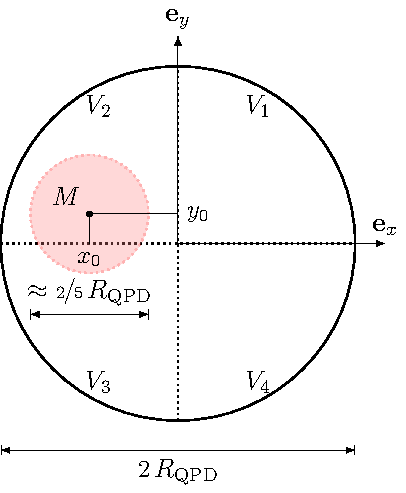
\includegraphics[]{Plots/cache/QPD.pdf}
  \caption{Sketch of quadrant photo detectors for $x$-$y$ detection with center 
  of laser image $M$ at $(x_{0}, y_{0})$.}
  \label{fig:Th-QPD}
\end{figure}

The received intensity $V_{i}$ per quadrant can be evaluated with four 
integrals over the respective areas
\begin{subequations}
\begin{align}
  V_{\MR{1}} & = \int_{0}^{\sfrac{\pi}{2}}\int_{0}^{\RA}
  \tilde{\intensity}\left( r\cos\varphi, r\sin\varphi 
  \right)\,r\,\dd{r}\dd{\varphi}
  \label{eq:Th-V1}
  \\[3mm]
  V_{\MR{2}} & = \int_{\sfrac{\pi}{2}}^{\pi}\int_{0}^{\RA}
  \tilde{\intensity}\left(r\cos\varphi, 
  r\sin\varphi\right)\,r\,\dd{r}\dd{\varphi}
  \label{eq:Th-V2}
  \\[3mm]
  V_{\MR{3}} & = \int_{\pi}^{\sfrac{3\pi}{2}}\int_{0}^{\RA}
  \tilde{\intensity}\left(r\cos\varphi, 
  r\sin\varphi\right)\,r\,\dd{r}\dd{\varphi}
  \label{eq:Th-V3}
  \\[3mm]
  V_{\MR{4}} & = \int_{\sfrac{3\pi}{2}}^{2\pi}\int_{0}^{\RA}
  \tilde{\intensity}\left(r\cos\varphi, 
  r\sin\varphi\right)\,r\,\dd{r}\dd{\varphi}
  \label{eq:Th-V4}
\end{align}
\end{subequations}
where we used polar integration and polar coordinates $x=r\cos\varphi$ and 
$y=r\sin\varphi$.

\begin{figure}[tbp]
  \centering
  % \tikzsetnextfilename{V_quadrant}
%%%%%%%
% READ TABLE
%%%%%%%
\pgfplotstableread{\relPath/10_Figures/TikZ/V_mat.dat}{\data}

\renewcommand{\tikzHelper}{
  \draw[black] (-1,0,0)--(1,0,0);
  \draw[black] (0,-1,0)--(0,1,0);
  \draw[black] (0,0,0) circle (1);
  }

\pgfplotsset{%
    colormap={bwr}{
      color=(blue);
      color=(white);
      color=(red);
    }%
}
%%%%%%%%%%%%%%%%%%%%%%%%%%%%%%%%%%
% Voltages per Quadrant
%%%%%%%%%%%%%%%%%%%%%%%%%%%%%%%%%%

\begin{tikzpicture}
  \begin{groupplot}[view={0}{90},
    % xlabel=$x$,
    % ylabel=$y$,
    height=5cm,
    width=5cm,
    point meta min=0,
    point meta max=1,
    colormap={}{ gray(0cm)=(1); gray(1cm)=(0);},
    group/xlabels at = edge bottom,
    group style = {
      group size = 2 by 2,
      horizontal sep=5mm,
      vertical sep=5mm,
      xlabels at = edge bottom,
      ylabels at = edge bottom
    }]

    \nextgroupplot[
      xticklabels={,,},
      ylabel={$\sfrac{y_{0}}{\RA}$},
    ]
        \addplot3[surf,mesh/rows=99,shader=interp] table[x=x,y=y,z=V4] {\data};
        \tikzHelper

    \nextgroupplot[
      yticklabels={,,},
      xticklabels={,,},
      colorbar right,
      every colorbar/.append style={
        ylabel={Normalized Voltage $\normalized{V}$},
        height=2*\pgfkeysvalueof{/pgfplots/parent axis height}+
        \pgfkeysvalueof{/pgfplots/group/vertical sep}}]
        \addplot3[surf,mesh/rows=99,shader=interp] table[x=x,y=y,z=V1] {\data};
        \tikzHelper

    \nextgroupplot[
      xlabel={$\sfrac{x_{0}}{\RA}$},
      ylabel={$\sfrac{y_{0}}{\RA}$},
    ]
        \addplot3[surf,mesh/rows=99,shader=interp] table[x=x,y=y,z=V3]
        {\data};
        \tikzHelper

    \nextgroupplot[
      xlabel={$\sfrac{x_{0}}{\RA}$},
      yticklabels={,,},
    ]
        \addplot3[surf,mesh/rows=99,shader=interp] table[x=x,y=y,z=V2] {\data};
        \tikzHelper


  \end{groupplot}
\end{tikzpicture}

  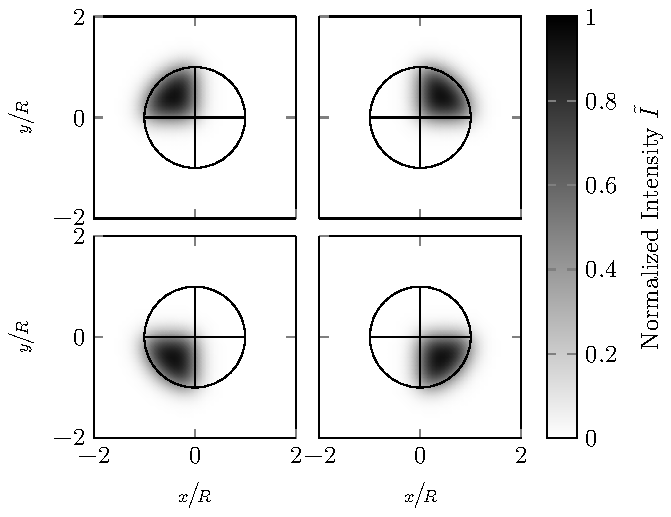
\includegraphics[]{Plots/cache/V_quadrant.pdf}
  \caption{Intensity per quadrant for various positions of laser image middle 
    point $M$ (see \cref{eq:Th-V1,eq:Th-V2,eq:Th-V3,eq:Th-V4}). The top right 
  plot is $V_{1}$, top left $V_{2}$, bottom left $V_{3}$, bottom right 
$V_{4}$.}
  \label{fig:Th-quadrant_Intensity}
\end{figure}

If the particle moves within the trap the center of the laser image $M$ on the 
QPDxy also moves. \cref{fig:Th-quadrant_Intensity} shows the intensity per 
quadrant for different center positions. As expected, each quadrant is 
measuring the highest intensity whenever most of the laser image is over the 
respective area.

With these for separate values for $V_{1}$ through $V_{4}$, one can create a 
measure that is proportional to the movement of the laser image center $M$ 
along the $\ex$- and $\ey$-direction, respectively. The measure is a addition 
and subtraction of the quadrants along one direction
\begin{subequations}
\begin{align}
  V_{\MR{x}} & = \left( V_{\MR{1}}+V_{\MR{4}} \right) - \left( V_{\MR{2}} + 
  V_{\MR{3}}  \right)
  \label{eq:Th-Vx} \\
  V_{\MR{y}} & = \left( V_{\MR{1}}+V_{\MR{2}} \right) - \left( V_{\MR{3}} + 
  V_{\MR{4}}  \right)
  \label{eq:Th-Vy} \\
  V_{\MR{t}} & = V_{\MR{1}}+V_{\MR{2}} + V_{\MR{3}} + V_{\MR{4}}.
  \label{eq:Th-Vt}
\end{align}
\end{subequations}

 \begin{figure}
  \centering
  \begin{subfigure}[b]{0.35\textwidth}
    \centering
    % \caption{$V_{\MR{x}}$}
    % \tikzsetnextfilename{QPDx}

\renewcommand{\tikzHelper}{
  \draw[black] (-1,0,0)--(1,0,0);
  \draw[black] (0,-1,0)--(0,1,0);
  \draw[black] (0,0,0) circle (1);

  \draw[black, dotted] (-1.5,0,0) -- (1.5,0,0);
  \draw[black, dotted] (-1.5,-0.6,0) -- (1.5,-0.6,0);
  \draw[black, dotted] (-1.5,0.6,0) -- (1.5,0.6,0);
}

\begin{tikzpicture}
  \begin{axis}[view={0}{90},
      xlabel=$\sfrac{x_{0}}{\RA}$,
      ylabel=$\sfrac{y_{0}}{\RA}$,
      point meta min=-1,
      point meta max=1,
      height=48mm,
      width=48mm,
      colormap/PuOr-11,
      colorbar,
      colorbar horizontal,
      colorbar style={
        title={\footnotesize Normalized Voltage $\normalized{V}_{x}$},
        at={(0,1.4)},
        anchor=north west,
        xtick={-1,0,1},
      }
    ]
      \addplot3[surf,mesh/rows=99,shader=interp] table[x=x,y=y,z=Vy] 
      {\relPath/10_Figures/TikZ/V_mat.dat};
    \tikzHelper
  \end{axis}
\end{tikzpicture}

    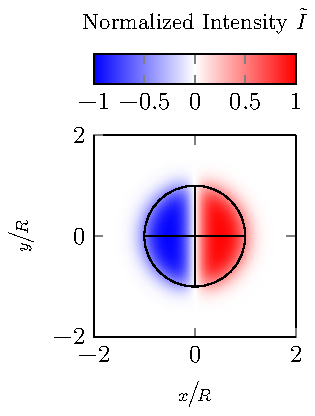
\includegraphics[]{Plots/cache/QPDx.pdf}
    \label{fig:Th-QPDx}
  \end{subfigure}
  \hfill
  \begin{subfigure}[b]{0.3\textwidth}
    \centering
    % \caption{$V_{\MR{y}}$}
    % \tikzsetnextfilename{QPDy}

\renewcommand{\tikzHelper}{
  \draw[black] (-1,0,0)--(1,0,0);
  \draw[black] (0,-1,0)--(0,1,0);
  \draw[black] (0,0,0) circle (1);
}

\pgfplotsset{%
    colormap={bwr}{
      color=(blue);
      color=(white);
      color=(red);
    }%
}

\begin{tikzpicture}
  \begin{axis}[view={0}{90},
      xlabel=$\sfrac{x}{\R}$,
      yticklabels={,,},
      point meta min=-1,
      point meta max=1,
      height=50mm,
      width=50mm,
      colorbar,
      colorbar horizontal,
      colorbar style={
        title={\footnotesize Normalized Intensity $\normalized{\intensity}$},
        at={(0,1.4)},
        anchor=north west,
        xtick={-1,-0.5,...,1},
      }
    ]
      \addplot3[surf,mesh/rows=51,shader=interp] table[x=x,y=y,z=Vx] 
      {\relPath/10_Figures/TikZ/V_mat.dat};
    \tikzHelper
  \end{axis}
\end{tikzpicture}

    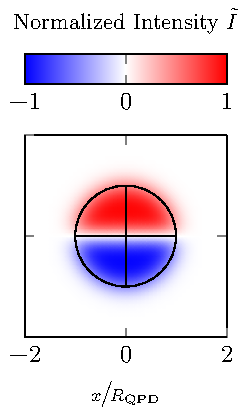
\includegraphics[]{Plots/cache/QPDy.pdf}
    \label{fig:Th-QPDy}
  \end{subfigure}
  \hfill
  \begin{subfigure}[b]{0.3\textwidth}
    \centering
    % \caption{$V_{\MR{t}}$}
    % \tikzsetnextfilename{QPDt}

\begin{tikzpicture}
  \begin{axis}[view={0}{90},
      xlabel=$\sfrac{x_{0}}{\RA}$,
      yticklabels={,,},
      height=48mm,
      width=48mm,
      colormap name=WhiteOr,
      colorbar,
      colorbar horizontal,
      colorbar style={
        title={\footnotesize Normalized Voltage $\normalized{V}_{t}$},
        at={(0,1.4)},
        anchor=north west,
        xtick={0,0.5,1},
      }
    ]
      \addplot3[surf,mesh/rows=99,shader=interp] table[x=x,y=y,z=V] 
      {\relPath/10_Figures/TikZ/V_mat.dat};

  \draw[black] (-1,0,0)--(1,0,0);
  \draw[black] (0,-1,0)--(0,1,0);
  \draw[black] (0,0,0) circle (1);

  \draw[black, dotted] (-1.5,0,0) -- (1.5,0,0);
  \draw[black, dotted] (-1.5,-0.6,0) -- (1.5,-0.6,0);
  \draw[black, dotted] (-1.5,0.6,0) -- (1.5,0.6,0);
  \end{axis}
\end{tikzpicture}

    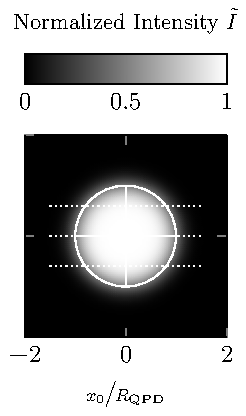
\includegraphics[]{Plots/cache/QPDt.pdf}
    \label{fig:Th-QPDt}
  \end{subfigure}
  \caption{QPD measure $V_{\MR{x}}$ (left;~\cref{eq:Th-Vx}), $V_{\MR{y}}$ 
    (center;~\cref{eq:Th-Vy}), and $V_{\MR{t}}$ (right;~\cref{eq:Th-Vt}) for 
    various positions of laser image middle point $M$. The dotted horizontal 
    lines are at $y=\sfrac{-0.6}{R_{\MR{QPD}}}$, $y=\sfrac{0}{R_{\MR{QPD}}}$, 
  and $y=\sfrac{0.6}{R_{\MR{QPD}}}$ respectively.}
  \label{fig:Th-QPDs}
 \end{figure}

As for the measured intensity per quadrant, the measured values are highest if 
the laser image is over the respective quadrants (see \cref{fig:Th-QPDs}). 
However, since $V_{\MR{x}}$ and $V_{\MR{y}}$ are composed by addition and 
subtraction of the strictly positive values $V_{i}$ the magnitude can now also 
be negative.

In \cref{fig:Th-voltages_over_x} the three measures are plotted over $x_{0}$ 
for three fixed values of $y_{0}$. This plot looks the same if $x_{0}$ is fixed 
and $y_{0}$ is the changing variable. Additionally the curves $V_{\MR{x}}$ and 
$V_{\MR{y}}$ change their behavior. It is clear, that there is a linear region 
for which a little movement of the laser image middle point $M$ is converted 
into a proportional change in the measured intensity on the QPD. However, this 
\emph{linear regime} from $-0.15\,R_{\MR{QPD}}$ to $0.15\,R_{\MR{QPD}}$ is 
rather little. Therefore, it is very important to check and adjust the offset 
of the QPD before each measurement to ensure interpretability of the results.

Noteworthy is also that for values of $\sfrac{\abs{x_{0}}}{R_{\MR{QPD}}} > 0.5$ 
a further outwards movement does not lead to an increase of the respective 
measure but to a decrease. If just one measure, here $V_{\MR{y}}$, is taken 
into account then this decrease ($\sfrac{x_{0}}{R_{\MR{QPD}} > 0.5}$) is not 
distinguishable from the increase coming from the middle 
($\sfrac{x_{0}}{R_{\MR{QPD}} < 0.5}$). However, by also looking at the 
evolution of $V_{\MR{t}}$ it is possible to identify in which direction the 
laser image is moving on the QPD because this measure does not change its 
magnitude between $\sfrac{\abs{x_{0}}}{R_{\MR{QPD}}} < 0.5$.

\begin{figure}[tbp]
  \centering
  % \tikzsetnextfilename{voltages_over_x}
%%%%%%%
% READ TABLE
%%%%%%%
\pgfplotstableread{\relPath/10_Figures/TikZ/V_line.dat}{\data}

\renewcommand{\tikzHelper}{
  \filldraw[black!10!, opacity=0.5] (-1,-1.1) rectangle (1,1.1);
}

\begin{tikzpicture}
\begin{groupplot}[
    group style={
        group name=myplot,
        group size= 1 by 3,
        vertical sep=8mm,
        },
    height=40mm,
    width=120mm,
    ymin=-1.1,
    ymax=1.1,
    ]
    \nextgroupplot[
    % ylabel={$\tilde{I}$},
      xticklabels={,,},
      title={$y = \sfrac{-0.64}{\RA}$},
      title style={yshift=-2mm},
      ]
      \tikzHelper
      \addplot[dotted] table[x=x,y=Vx_1] {\data};
      \addlegendentry{$V_{\MR{x}}$};
      \addplot[] table[x=x,y=Vy_1] {\data};
      \addlegendentry{$V_{\MR{y}}$};
      \addplot[dashed] table[x=x,y=V_1] {\data};
      \addlegendentry{$V_{\MR{t}}$};
    \nextgroupplot[
      % ylabel={$\tilde{I}$},
      title={$y = \sfrac{0}{\RA}$},
      title style={yshift=-2mm},
      xticklabels={,,},
      ylabel={Normalized Intensity $\normalized{\intensity}$},
      every axis y label/.append style={at=(ticklabel cs:0.5)}
      ]
      \tikzHelper
      \addplot[dotted] table[x=x,y=Vx_2] {\data};
      \addplot[] table[x=x,y=Vy_2] {\data};
      \addplot[dashed] table[x=x,y=V_2] {\data};
    \nextgroupplot[
      % ylabel={$\tilde{I}$},
      xlabel={$\sfrac{x}{\RA}$},
      title={$y = \sfrac{0.64}{\RA}$},
      title style={yshift=-2mm},
      ]
      \tikzHelper
      \addplot[dotted] table[x=x,y=Vx_3] {\data};
      \addplot[] table[x=x,y=Vy_3] {\data};
      \addplot[dashed] table[x=x,y=V_3] {\data};
\end{groupplot}
\end{tikzpicture}

  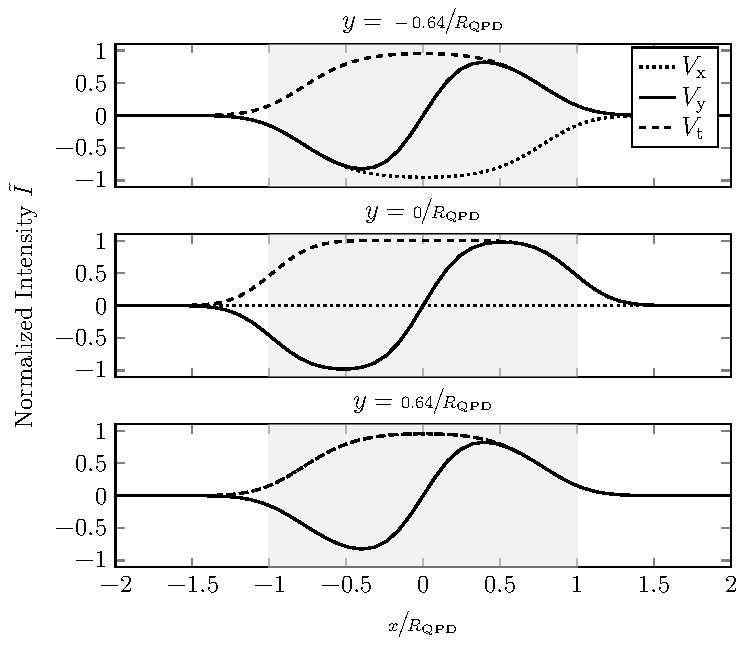
\includegraphics[]{Plots/cache/voltages_over_x.pdf}
  \caption{QPD measure $V_{\MR{x}}$ (\cref{eq:Th-Vx}), $V_{\MR{y}}$
    (\cref{eq:Th-Vy}), and $V_{\MR{t}}$ (\cref{eq:Th-Vt}) over $x_{0}$ for 
  three fixed values of $y_{0}$. The light shaded gray area marks the 
boundaries of the QPD and the dark shaded gray area the linear region of the 
QPD from $-0.15\,R_{\MR{QPD}}$ to $0.15\,R_{\MR{QPD}}$.}
  \label{fig:Th-voltages_over_x}
\end{figure}



\cleardoublepage
\renewcommand{\relPath}{SECTION/30_Timeconstant}
 
\chapter[Dynamic Timeconstant Measurement]{Dynamic Measurement of the Acoustic 
Streaming Time Constant utilizing an Optical Tweezer}\label{ch:timeconstatn}
\textit{This chapter resulted from a collaboration between the Bioanalytics 
  Group, Department of Biosystems Science and Engineering, ETH Zurich, Basel, 
  and the Mechanics and Experimental Dynamics group, Department of Mechanical 
  and Process Engineering, ETH Zurich, Zurich. We successfully combined the 
  expertise of both groups, namely droplet microfluidics and cell culturing 
  (Dominik Haidas), and acoustic particle manipulation (Michael Gerlt). The 
  chapter has been published previously in the journal Biomicrofluidics:
\footnote{: DOI: 10.1103/PhysRevE.104.025104, reproduced with permission, 
copyright 2020 AIP Publishing.}}

\vspace{5mm} \noindent
C. Goering and J. Dual, "Dynamic measurement of the acoustic streaming time 
constant utilizing an optical tweezer", Physical Review E, 2021, \textbf{104}, 
025104.


\section{Abstract}
Two orthogonal standing acoustic waves, generated by piezoelectric excitation, 
can form a two-dimensional pressure field in microfluidic devices. A phase 
difference of the excitation waves can be employed to rotate spherical 
\si{\micro\meter}-sized silica particles by a torque mediated through the 
viscous boundary $\delta$ around the particle.

The measurement of the rotational rate is, so far, limited to high-speed cameras 
and their frame rate, and gets increasingly difficult when the sphere gets 
smaller.  We report here a new method for measuring the rotational rate of 
\si{\micro\meter} sized spherical particles. We utilize an optical trap with 
high-speed position detection to overcome the frame rate limitation of wide 
field image recording. The power spectrum of an optically trapped, rotating 
particle reveals additional peaks corresponding to the rotational frequencies -- 
compared to a non-rotating particle. We validate our method at low rotational 
rates against high-speed video observation. 

To demonstrate the potential of this method we addressed a recent controversy 
about the rotation of particles with a relatively large VBL 
$\delta$. We measured steady-state rotational rates up to \SI{229}{\hertz} 
(\SI{13.8e3}{\rpm}) for a particle with a radius $R \approx \delta$.  Recent 
numerical research suggests that in this regime the existing theoretical 
approach (valid for $R\gg\delta$) overpredicts the steady-state rotational rate 
by a factor of 10.  With our new method we also confirm the numerical results 
experimentally.

\section{Introduction\label{sec:TC-introduction}}

In recent years, acoustofluidics has provided many powerful tools. Due to being 
contact-less, label-free, and biocompatible 
\cite{Antfolk2015,Abdulla2020,Zielke2020,Binkley2020,Cai2020}, acoustofluidic 
manipulation can be used in medical applications for cancer research
\cite{Antfolk2015,Abdulla2020,Zielke2020,Binkley2020}, Alzheimer research 
\cite{Cai2020}, targeted drug delivery \cite{Bose2015}, and for pumping medical 
fluids \cite{Wu2019}. In addition, there are biological 
\cite{Gerlt2020,Xie2019} and engineering applications (e.g., micro-pumping 
\cite{Wu2019,Huang2014,Lin2019,Ozcelik2021}).

Most of these applications utilize the acoustic radiation force (ARF) to 
manipulate objects on the micro-scale. The ARF is a second-order time-averaged 
effect that arises from the interaction of an acoustic field scattered at an 
object surface and a background acoustic field 
\cite{Doinikov1994Rigid,Hasegawa1969,Yosioka1955,Gorkov1962,Bruus2012}.
These objects can be solid particles, air bubbles, fluid droplets, biological 
samples, as long as their material properties (density $\rho$ and speed of 
sound $c$) are different from the surrounding medium. However, there coexists 
a fluid motion called acoustic streaming (AS) 
\cite{Nyborg1965,Kolb1956,Nyborg1953}. This motion can arise either from
viscous losses in the fluid (Eckhart type streaming \cite{Eckart1948}) or it 
can arise in the viscous boundary layer at a fluid to wall interface 
(Schlichting and Rayleigh streaming \cite{Riley1998,Schlichting1932}).


The theoretical derivations usually describe the steady-state of the AS field. 
A theoretical numerical study \cite{Muller2015} investigated the temporal build 
up of the ARF and AS field. In contrast to the ARF, the viscous drag force 
arising from AS is independent of the object material properties because it is 
a motion of the fluid. The AS direction coincides with the direction of the 
relative motion between fluid and particle.

For a spherical object of radius $R$, the drag force in laminar flow scales 
linearly with the object radius $\FAS \propto R$. In contrast to the $\FAS$, 
the ARF scales with the volume $\FARF \propto \R^{3}$ \cite{Bruus2012-10}.  
Based on the fluid and the object material properties, the $\FARF$ will 
dominate over the $\FAS$ if the radius $\R$ is greater than the critical radius 
$\R_{\text{crit}}$, where $\FAS = \FARF$ holds. The direction of $\FAS$ can be 
different from the $\FARF$. Therefore, the $\FAS$ is usually undesired.

The ARF and the AS occur not only in the bulk of the fluid, but also on sharp 
edges of a device \cite{Doinikov2020a,Doinikov2020b,Leibacher2015,Nama2016}. 
So-called micro-streaming around the surface of a spherical particle can even 
cause a sign inversion of the ARF if the viscous boundary layer $\delta$ is 
sufficiently large \cite{Baasch2019}. However, there are applications that take 
advantage of the AS \cite{Antfolk2014,Mao2017,Hao2020}: a complete overview of 
AS applications can be found in \cite{Wiklund2012a}.

In literature, it is well understood how long it takes until the acoustic 
field, and hence the ARF, needs to build up \cite{Muller2015} and how long the 
particle focusing takes \cite{Bruus2012-10}. However, it is still not fully 
clear how long it takes for the AS to build up, and what the definition for the 
analytical AS time constant is. In the acoustofluidics community, it is 
generally accepted that the build up for the AS field takes longer than the 
build up of the ARF. By using a pulsed actuation of the acoustic field and 
therefore exploiting this time offset, \citeauthor{Hoyos2013} prevented the 
build up of AS \cite{Hoyos2013,Castro2016}. They varied the number of periods 
for which the acoustic actuation is switched on and off, respectively. They 
experimentally showed that for a ratio of about 1 to 1 between 500 on- and 500 
off-periods the streaming velocity is less than 50\% of its steady-state 
magnitude while the ARF is not affected by that much.

\citeauthor{Muller2015} studied the build up of the acoustic energy density and 
streaming velocity with a numerical model \cite{Muller2015}. Their model 
consisted of a fluid cavity without any surrounding structure such as the 
cavity walls. They found numerically that indeed the ARF builds up 
significantly faster than the AS. However, the simulations with a pulsed 
actuation of different ratios of on- to off-periods did not prevent the build 
up of AS because its decay -- as the build up -- is slow compared to the ARF. 
The streaming builds up significantly slower during the on-periods, however, it 
does not decay to its initial value during the off-periods. Over time the 
influence of AS increases because the ARF alternates between some magnitude in 
the on-periods and zero in the off-periods. This implies, that the simulation 
of \citeauthor{Muller2015} could not explain the experimental results by 
\citeauthor{Hoyos2013}.

In this work, we experimentally measure the time until a \Dtwo~spherical 
silicon-dioxide (\SiO) particle moves with constant velocity when accelerated 
by the ARF and AS. Instead of using a camera, we utilize a data acquisition 
board (DAQ) with a sampling frequency of $f_{\text{s}} = \SI{1.25}{\MHz}$ to 
measure the relative particle trajectory as soon as the ultra-sound (US) is 
switched on. This high sampling frequency $f_{\text{s}}$ yields a high 
temporal resolution of $ \Dt = \SI{0.8}{\us}$. Considering the acoustic 
excitation frequency $\fex = \SI{4.015}{\MHz}$, we sample at least every fourth 
excitation period.

The optical tweezer (OT) for this study has already been successfully applied 
in the fields of acoustofluidics for stationary force measurements within a 
microfluidic chip \cite{Lamprecht2016,Lakaemper2015} as well as acoustic 
viscous torque investigations \cite{Lamprecht2021}. Here, we characterize in a 
first step the stationary force field in the bulk of the device to ensure, that 
we measure in a second step the time resolved build up of AS and the ARF 
separately and not their superposition. The separation is done by choosing a 
particle position within the acoustic field, where the $\FAS$ and $\FARF$ are 
orthogonal to each other. In order to measure in the second step solely the 
effects of the acoustic field on the particle and not the characteristics of 
the OT, we alter the usual trapping setup. The modification is that the 
particle is released from the OT before the acoustic excitation starts and 
retrapped after it.  Hence, during the measurement just gravity and the forces 
of the acoustic field act upon the particle. With our modified trapping setup, 
we are able to measure precisely the ARF and AS induced movement of a single 
particle in the bulk of the fluid.

Our manuscript is structured as follows: in \cref{sec:TC-theory} we derive and 
list all time constants in our system and we compute the traveled distances of 
a free floating particle in an acoustic field. Those influences need to be 
considered for our measurement protocol. In addition, we perform numerical AS 
simulations of our device to further understand the AS field; in 
\cref{sec:TC-experimental-setup} we explain our experimental setup and its 
modifications; in \cref{sec:TC-experimental-procedure} we show the results of the 
stationary force measurement, before explaining our time evolution measurement 
protocol and the data post-processing; and in \cref{sec:TC-results} we show and 
discuss the results of this study.




\section{Preliminary Theoretical Considerations\label{sec:theory}}
\subsection{Time Constants}

\begin{figure}[ht]
  \centering
  \def\svgwidth{\figWidth}
  \svginput{\relPath/10_Figures/LaTeX/Device.pdf_tex}
  \caption{Sketch of device. The light-gray area is the silicon channel walls, 
    the light-blue is the fluid cavity, and the dark-gray block the 
    piezoelectric element. The total length of the device is \SI{76}{\mm}. All 
dimensions are as listed in \cref{tab:device-dimensions}.}\label{fig:device}
\end{figure}

\begin{table}
  \centering
  \begin{tabular}{l *{8}{x{10mm}}}
    \toprule
    \toprule
    Symbol & $W$ & $H$ & $W_{D}$ & $H_{T}$ & $H_{B}$ & $l$ & $w$ & $h$ \\
    Value [\si{\milli\meter}] & 3 & 0.1 & 26 & 0.13 & 0.9 & 20 & 4 & 0.5\\
    \bottomrule
    \bottomrule
  \end{tabular}
  \caption{Overview of device dimensions}\label{tab:device-dimensions}
\end{table}


In our experiments there are multiple time constants that need to be considered. 
In the center of interest are the evolution of the ARF and the AS field. The 
acoustic energy $E_{\text{ac}}$, and hence the ARF, has the characteristic 
time constant \cite{Muller2015}
\begin{equation}
    \tarf = \frac{Q}{\omega_{0}} = \frac{Q}{2\pi\,\fex}
  \label{eq:tau-arf}
\end{equation}
with $Q$ being the quality factor of the considered acoustic pressure mode and 
$\fex$ the excitation frequency. For the AS field, a theoretical expression for 
the time constant does not exist. Nevertheless, \citeauthor{Muller2015} report 
a \emph{momentum diffusion time}
\begin{equation}
  \tas = \frac{1}{2\nu}  L^{2} = \frac{\rhof}{2\muef} L^{2}
  \label{eq:tau-nu}
\end{equation}
as the time constant for the AS field. Here, $L$ is half the radius of a 
streaming roll, $\nu=\sfrac{\muef}{\rhof}$ the kinematic viscosity, $\rhof$ the 
density, and $\muef$ the dynamic viscosity of the fluid. This formula is except 
for a factor of $\sfrac{1}{2}$ the same to $\tiner$ (equation 1.88) in 
\cite{Bruus2015}, which is the time a Poisseuille flow needs to fully stop in a 
circular tube of radius $L$ after the immediate removal of its driving 
pressure. To the best of the authors' knowledge, there is so far no better 
approximation for the time constant of the AS field.

When a particle is stably trapped, our OT has the properties of a linear 
mechanical spring \cite{Lamprecht2016}. This spring-like behavior of the OT has 
also a time constant until an acting force moves the trapped particle in its 
equilibrium position. The stiffness of the OT $k_{i}$ is linearly related to a 
characterization parameter of the OT called the cut-off frequency $f_{\text{c}} 
= \sfrac{k_{i}}{2\pi\,\gamma}$ with $\gamma$ being Stokes' drag coefficient 
\cite{Lamprecht2016,Lamprecht2017}. This frequency is the \SI{-3}{\dB} point 
in the Brownian motion power spectrum (more detail in 
\cite{Lakaemper2015,Lamprecht2016}). We can therefore compute the time 
constant of the OT as
\begin{equation}
  \tOT = \frac{1}{2\pi\,f_{c}}.
  \label{eq:tau-OT}
\end{equation}
Lastly, our DAQ system has the time constant $\tqpd$ which describes how fast we 
can measure a sudden change in laser intensity of the OT. This parameter is 
found by changing the laser intensity at a precise point in time and then 
extracting the temporal difference until the DAQ measures it. 

With the parameters of our experiment (see \cref{tab:parameters}) the mentioned 
time constants are as listed in \cref{tab:time-constants}. Hence, with the 
usual trapping mode of the OT, we cannot measure the ARF and AS because $\tOT 
\approx \tas$ and $\tOT\gg\tarf$. In the limit of zero laser power there is no 
trapping potential and hence $\tarf$ and $\tas$ can be measured.

\begin{table}
  \centering
  \begin{tabular}{lccr}
    \toprule
    \toprule
    {\bfseries Parameter} & {\bfseries Symbol} & {\bfseries Value} & {\bfseries 
    Unit}\\
    \midrule
    \textbf{Fluid} & & \\
    Density & $\rhof$ & 1000 & \si{\kg\per\cubic\meter} \\
    Speed of sound & $\cfl$ & 1500 & \si{\m\per\s} \\
    Compressibility & $\kappa_{\text{f}}$ & 4.4E-10 & \si{\per\pascal} \\
    Dynamic viscosity & $\muef$ & 890 & \si{\micro\pascal\second} \\
    Kinematic viscosity & $\nu_{\text{f}}=\sfrac{\muef}{\rhof}$ & 0.890 & 
    \si{\square\mm\per\second} \\
    \midrule
    \textbf{Particle} & & \\
    Density & $\rhop$ & 1850 & \si{\kg\per\cubic\meter} \\
    Radius & $\Rtwo$ & 1.03 & \si{\um}\\
    Radius & $\Rfour$ & 2.195 & \si{\um}\\
    Compressibility & $\kappa_{\text{p}}$ & 1.6E-11 & \si{\per\pascal} \\
    \midrule
    Device quality factor & $Q$ & 36 & - \\
    Corner frequency of OT & $f_{\text{c}}$ & $\approx 100$ & \si{\hertz} \\
    \midrule
    Excitation frequency & $\fex$ & 4.015 & \si{\MHz} \\
    \bottomrule
    \bottomrule
    
  \end{tabular}
  \caption{Symbols and physical properties of the fluid, the particle, and the 
    experimental setup. The quality factor $Q$ is extracted from an admittance 
    measurement of the device filled with water and fixed in the microscope as 
for all measurements. The magnitude of $f_{\text{c}}$ is the usual value in 
stationary force measurements for the OT.}\label{tab:parameters}
\end{table}

\begin{table}
  \centering
  \begin{tabular}{l S[table-format=7.5]S[table-format=7.1]}
    \toprule
    \toprule
    {\bfseries Symbol} & {\bfseries $\tau_{i}$ [\si{\ms}]} & {\bfseries 
    $\sfrac{\tau_{i}}{t_{0}}$ [-]}  \\
    \midrule
    $\tOT$ & 1.59 & 6383.9 \\
    $\tqpd$ & 0.050 & 200.8 \\
    $\tarf$ & 0.0014 & 5.6 \\
    $\tas\vert_{L=\sfrac{H}{2}}$ & 1.44 & 5781.6\\
    $\tas\vert_{L=\sfrac{H}{4}}$ & 0.35 & 1405.3\\
    $\tdrag$ & 0.00049 & 2.0 \\
    \midrule
    $\Dt_{\text{DAQ}}$ & 0.0008 & 3.2 \\
    \bottomrule
    \bottomrule
    
  \end{tabular}
  \caption{Overview of time constants $\tau_{\text{i}}$ for the system. The 
    values are obtained by using the values from \cref{tab:parameters} and 
    \cref{eq:tau-nu,eq:tau-arf,eq:tau-OT,eq:tau-drag}. $\tqpd$ is measured, 
    $\Dt_{\text{DAQ}} = \sfrac{1}{f_{\text{s}}}$, and 
$t_{0}=\sfrac{1}{\fex}$.}\label{tab:time-constants}
\end{table}

\subsection{Free Particle Motion}

If there is no trapping laser power, the spherical particle with mass $m$ will 
move in the fluid due to some acting force $F$; this force can be gravity, the 
ARF, the drag force from AS, or a combination of them. The one dimensional 
dynamic equation for the particle displacement $q$ far away from any walls is 
the same for the three spatial directions $\ex, \ey$ and $\ez$.
\begin{equation}
  \ddot{q} = - \frac{F}{m} - \frac{\gamma}{m}\,\dot{q} =
  - \tilde{F} - \frac{1}{\tdrag}\,\dot{q}
  \label{eq:free-fall}
\end{equation}
with $F$ being a force acting along the direction of $q$ and
\begin{equation}
  \tdrag = \frac{m}{\gamma} = \frac{V\,\rhop}{6\pi\,\R\,\muef}
  = \frac{2}{9}\,\R^{2}\,\frac{\rhop}{\muef}.
  \label{eq:tau-drag}
\end{equation}
Here, $\R$ is the particle radius, $V$ the particle volume, and $\rhop$ the 
particle density. In microfluidics the viscous effects dominate over the 
inertial effects \cite{Bruus2015}. Therefore, we neglect $\ddot{q}$ for further 
calculations. Solving the modified first order ordinary differential equation
\begin{equation}
    \dot{q}= - \tdrag\,\tilde{F} = -\frac{F}{m}\,\tdrag
  \label{eq:mod-free-fall}
\end{equation}
with the initial condition $q\vert_{t=0} = 0$, gives the linear relation $q(t) 
= - \tdrag\,\tilde{F}\,t$ with the integration constant being zero.

As already mentioned, we measure while there is no trapping potential of the 
OT. Therefore, on the particle act only gravity and the forces from the 
acoustic field. In our experiment we have for $F$ along $\ey$ a spatially 
varying force with a maximal value of \SI{0.5}{\pico\newton} and along $\ez$ 
the buoyancy corrected gravitational force $\tilde{m}g=V\,\left( \rhop-\rhof 
\right)\,g$ with a magnitude of \SI{38.2}{\femto\newton} and an acoustic force 
with a maximal value of \SI{0.25}{\pico\newton} (for acoustic force magnitudes 
see \cref{fig:2um_map}). As we will explain later (see 
\cref{sec:experimental-procedure}), we have \SI{25}{\ms} without any laser 
power where the particle will solely move due to gravity and then \SI{30}{\ms} 
of US excitation where also the acoustic forces are acting.

Hence, a spherical \SiO~$\Rtwo=\SI{1.03}{\um}$~particle will have moved 
$0\Rtwo$ along $\ey$ and $0.05\Rtwo$ along $\ez$ after $\SI{25}{\ms}$ with just 
gravity acting. And, after $\SI{55}{\ms}$, when there are additionally 
constant acoustic forces, the particle will have traveled distances of 
$0.84\Rtwo$ and $0.54\Rtwo$ along $\ey$ and $\ez$, respectively. For the 
latter, $0.54\Rtwo$ is the sum of $0.12\Rtwo$ due to gravity and $0.42\Rtwo$ 
due the force from the acoustic field.

\subsection{Numerical Streaming Simulations}

To understand the influences and implications of the AS on our measurements, we 
simulate with {\ttfamily COMSOL Multiphysics 5.6} (COMSOL Inc., Stockholm, 
Sweden) 2 two-dimensional structures that relate to the experimental device; 
one with just the fluid cavity as the baseline model (cavity-only model); and 
the other with added structure around the cavity to reflect our real device 
(whole-device model). See \cite{supplemental} for both models as one {\ttfamily 
.mph} file. For both we follow the work of \citeauthor{Muller2015} 
\cite{Muller2015} in terms of the fluid mesh size.

\afterpage{
  \vspace*{\fill}
\begin{figure}[H]
  \centering
  \begin{subfigure}{\figWidthDouble}
    \centering
      \caption{Streaming simulation for cavity-only model at $f_{\text{max}} = 
      \SI{3.987}{\MHz}$.}\label{subfig:JC-streamingrolls}
    \def\svgwidth{\figWidthDouble}
    \textsf{\tiny % that is for the added unit @ the axis
    % \input{10_Figures/LaTeX/JC-streaming-rolls.pdf_tex}
    \svginput{\relPath/10_Figures/LaTeX/JC-streaming-rolls_paraview.pdf_tex}}
    \end{subfigure}\\%k
  \begin{subfigure}{\figWidthDouble}
    \centering
    \caption{Streaming simulation for whole-device model at $f_{\text{max}} = 
    \SI{3.745}{\MHz}$. The gray area is the structure around the 
  cavity.} \label{subfig:FD-streamingrolls}
    \def\svgwidth{\figWidthDouble}
    \textsf{\tiny % that is for the added unit @ the axis
    \svginput{\relPath/10_Figures/LaTeX/FD-streaming-rolls_paraview.pdf_tex}}
    % \input{10_Figures/LaTeX/FD-streaming-rolls.pdf_tex}
  \end{subfigure}
  \caption{Results for streaming simulations of a cavity-only model (a) and a 
    model with surrounding structure (b). The colormap shows the total acoustic 
    pressure and the white arrows the streaming flow. For both simulations 
    $f_{\text{max}}$ is the frequency of maximal acoustic energy density 
    $E_{\text{ac}}$ for a pressure mode with 16 nodal lines. The pressure mode 
  for both simulations is the same besides the phase shift of 
$\pi$.}\label{fig:comsol-streaming}
\end{figure}
\vspace*{\fill}
  \clearpage
}

We model a two-dimensional $yz$ slice of the whole device as seen in 
\cref{fig:device} without the piezoelectric transducer (PZT) and its glue 
layer. Therefore this whole-device model consists of two glass, two silicon, 
and one water domain. We utilize the Solid Mechanics \comsol{solid} interface 
for the silicon and glass. For the cavity we employ the Creeping Flow 
\comsol{spf} interface with the spatial variation of the Reynolds Stress as 
source and the Stokes drift as the boundary condition. Also in the cavity, we 
use the Thermoviscous Acoustics \comsol{ta} interface. Lastly, we couple the 
Solid Mechanics with the Thermoviscous Acoustics via Thermoviscous 
Acoustic-structure Boundary \comsol{tsb}. The cavity-only model solely needs 
the Creeping Flow and the Thermoviscous Acoustics interface without 
multiphysics coupling.

Besides the added structure around the cavity, the main difference between the 
two models is the location of the excitation. The whole-device model has as 
boundary condition a prescribed displacement along $\ez$ of 
$z_{\text{BD}}=\SI{0.1}{\nm}$, where the PZT is glued onto the device. The 
cavity-only model, however, has a prescribed constant velocity of its left 
cavity wall along $\ey$ of $\dot{y}_{\text{BD}} = \SI{25}{\mm\per\second}$. 
This magnitude corresponds to the mean wall velocity of the whole-device model, 
where the excitation is at the PZT. With those two boundary conditions the 
acoustic pressure is \SI{310}{\kPa} for the whole-model and \SI{550}{\kPa} for 
the cavity-only model at their respective 16 nodal pressure line frequency with 
maximal acoustic energy density $E_{\text{ac}}$. The discrepancy in pressure 
amplitude comes from the applied boundary conditions of respective models.

The respective frequencies of maximal $E_{\text{ac}}$ 
(\SI{3.9876}{\MHz} and \SI{3.7450}{\MHz}) inside the cavity while having a 16 
nodal line mode were determined with a frequency sweep. This is the same mode 
we have in our experiment as well. For the streaming simulation, we employ a 
stationary study of the Creeping Flow interface that uses the results from the 
frequency domain study in its source term and as the boundary conditions.

\Cref{fig:comsol-streaming} shows the results for the pressure and streaming 
fields of both models. The magnifications correspond to the area where we 
perform our measurements in the experiment. One can see that the simulated 
pressure fields are qualitatively the same, however, the streaming fields 
differ to a great extent. The cavity-only simulation depicts spatially 
repetitive streaming rolls over the whole fluid domain. In the bulk of the 
fluid is Rayleigh streaming. However, near-boundary Schlichting streaming is 
not visible because the viscous boundary layer is relatively small. In contrast 
to that, the simulation for the whole-device model has a non-spatially 
repetitive streaming field. There are regions where its similar to the 
cavity-only model streaming field. But, the streaming pattern is non-repetitive 
and exhibits strong local differences. As a consequence, care must be taken to 
chose a measuring point where the $\FAS$ and $\FARF$ are orthogonal to each 
other to ensure no superposition of forces.

Although the clamping of the microscope setup and the oil immersion layer for 
the lens are excluded in the model with structure, one can see that the 
streaming field is a local, non-periodic effect, whereas the pressure field is 
spatially periodic. We expect that these tendencies remain the same when the 
clamping, the immersion layer, and the PZT are added.

\section{Experimental Setup\label{sec:TC-experimental-setup}}

\subsection{Optical Trap Setup}

Our OT has already been applied in several other publications 
\cite{Lamprecht2021,Lamprecht2017,Lamprecht2016,Lakaemper2015} to the field of 
ARF and AS measurements in bulk acoustic wave (BAW) devices. All components are 
described there extensively. We highlight here the position detection system 
and the modifications from the force measurement setup that were necessary for 
this study. These modifications are needed because we use one \SI{785}{\nm} 
near-infrared diode laser (LuxX 785-200, Omicron Laser, Rodgau-Dudenhofen, 
Germany) for the optical trapping and also for the optical position detection.  
We detect the position of the trapped particle relative to the trap center by 
monitoring the voltages of two quadrant photo diodes (QPD) placed in the back 
focal plane (see \cref{fig:TC-laserpath}). It is possible to resolve the movement 
of the particle in all three dimensions. However, the in-plane ($xy$) and the 
axial ($z$) position detection differ.

\begin{figure}[H]
  \centering
  \def\svgwidth{85mm}
  {\small
  \svginput{\relPath/10_Figures/LaTeX/Microscope.pdf_tex}
  }
  \caption{Shutter location in laser path and schematic of laser path through 
  microscope setup; full details on the setup in 
  \cite{Lamprecht2016,Lamprecht2017}.}\label{fig:TC-laserpath}
\end{figure}

For the $xy$ position the laser beam is focused onto the QPDxy (see also 
\cref{fig:TC-laserpath}) such that the spot diameter is about five times smaller 
than the opening aperture of the QPDxy \cite{Lamprecht2017}. An in-plane 
movement of the trapped particle changes the spot location on the QPDxy which 
results in a voltage change on the four quadrants. As long as the spot is 
within the QPD opening the spatial movement is linearly related to the QPD 
voltage. By summing and subtracting these four voltages from each other, one 
can get the values corresponding to a movement along $\ex$ and $\ey$ separately 
\cite{Lamprecht2017}.

For the axial $z$ position a second QPD is needed and this QPD is overfilled 
with the laser spot (see also \cref{fig:TC-laserpath}). When the particle moves 
axially the spot diameter changes its size. If the diameter decreases more 
intensity is measured by QPDz and leads to a higher voltage and vice versa. For 
small movements ($\Dz < \R$) the relation is linear \cite{Dreyer2004}.

When converting the measured voltage changes from QPDxy and QPDz to the 
particle displacement with unit of meters, the $xy$ voltage and the $z$ voltage 
have different scaling. The three voltage-meter conversion factors are found by 
calibrating the OT via the power spectrum analysis of the trapped particle 
Brownian motion \cite{Lamprecht2021,Lamprecht2016,Lakaemper2015}.

As discussed before, the time constant $\tOT$ of the OT is larger than the 
time constant for the ARF and AS (see \cref{tab:TC-time-constants}). Therefore, we 
need to switch the laser off and then monitor the particle trajectory without 
the trapping forces, in order to measure the time evolution of the particle 
movement and not the time constant of the optical trap. This means, the particle 
is not stably trapped while measuring. However, we need the laser light for 
the position detection on the QPDs. Therefore, we reduce the laser power to a 
minimum such that the resulting trapping forces are negligibly small. As a 
result of the low power, the voltage magnitude decreases significantly on the 
QPDs, such that it is not measurable anymore. Thus, we exchange the neutral 
density (ND) filters from the force measurement setup 
\cite{Lamprecht2016,Lamprecht2021} with the fast optical shutter FOS-NIR(1100) 
(LC TEC, Borlänge, Sweden). This filter is specified to open from 0\% to 90\% 
transmittance in less than \SI{15}{\ms} and close from 100\% transmittance to 
10\% in less than \SI{5}{\ms}. The ND filters and the shutter are needed to 
reduce the intensity on the QPDs and prevent overexposure and hence damage. 
The transmittance of the shutter can be controlled with the applied driving 
voltage. Before and after the measurements the shutter is almost completely 
closed to mimic the ND filters and opened for the actual measurement with 
reduced laser power.

Lastly, we operate the laser in the so-called \emph{analogue modulation} mode 
such that the output laser power is proportional to an externally applied DC 
voltage which is sampled with more than \SI{1.5}{\MHz} by the laser controller 
unit. The low power mode for the position detection is operated with less than 
\SI{0.5}{\mW}. The low voltage DC signal for the laser averaged \SI{84.13}{\mV} 
with a standard deviation of \SI{0.13}{\mV} providing a very consistent voltage 
and hence laser power. With this power the trapping potential is too weak to 
keep the particle inside the focus of the laser beam in any of the three 
spatial directions. The usual laser power for the stationary force measurements 
is between \SI{100}{\mW} and \SI{175}{\mW}.

\begin{figure}[H]
  \centering
  % \tikzsetnextfilename{daq-sync}
\begin{tikzpicture}
  \tikzset{nodestyle/.style={pos=0.0, above, anchor=south west}}
  % \draw[white, fill=black!10!white] (2.5,0) rectangle ++(1.5,3.5);
  % \draw[|<->|] (2.5,3.5) -- ++(1.5,0) node[midway,above=2mm,align=center] 
  % {\small Shutter open\\US on\\laser power low};

  % \draw[|<->|] (1.0, 0.5) -- ++(6.0,0) node[midway, above] {particle is free to 
  % float and move};
  % axis system
  \draw[thick,->] (-0.2,0) -- ++(6.5,0) node[anchor=north west] {$t$ 
  [\si{\milli\second}]};

  % time ticks
  \draw (0, 2pt) -- ++(0, -4pt) node[anchor=north] {$-25$};
  \draw (1.0, 2pt) -- ++(0, -4pt) node[anchor=north] {$-24$};
  \draw (2.5, 2pt) -- ++(0, -4pt) node[anchor=north] {$0$};
  \draw (4.0, 2pt) -- ++(0, -4pt) node[anchor=north] {$30$};
  \draw (5.0, 2pt) -- ++(0, -4pt) node[anchor=north] {$55$};
  \draw (6.0, 2pt) -- ++(0, -4pt) node[anchor=north] {$75$};

  % laser power
  \draw[dashed] (-0.5,2.7) -- node[nodestyle] {$P_{\text{trapping}}$} ++(1.5,0) 
  -- ++(0,-1.0) -- node[nodestyle] {$P_{\text{measure}}$} ++(5.0,0) -- 
  ++(0,1.0) -- ++(1,0) node[nodestyle] {laser};

  % shutter
  \draw[dotted] (-0.5,4) -- node[nodestyle] {closed} ++(0.5,0) -- ++(1.5,-1.5) 
  -- node[nodestyle] {open} ++(2.5,0) -- ++(1.5, 1.5) -- ++(1.5,0) 
  node[nodestyle] {shutter};

  % US
  \draw[] (-0.5, 0.2) -- node[nodestyle] {off} ++(3.0,0) -- ++(0,1) -- 
  node[nodestyle] {on} ++(2.5,0) -- ++(0,-1) -- node[nodestyle] {US} ++(1.5,0);


\end{tikzpicture}

  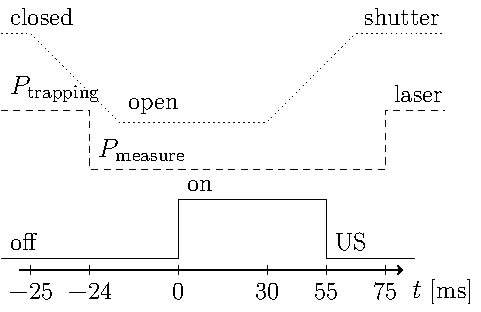
\includegraphics[]{/daq-sync.pdf}
  \caption{Schematic of controller timings for the shutter, the laser, and the 
      US. During the $P_{\text{measure}}$ state the particle is not trapped by 
  the OT. In the time interval $[\SI{0}{\ms}, \SI{30}{\ms}]$ (1) the shutter is 
  fully opened, (2) the US is switched on, and (3) the particle is free to 
  move. During this interval the measurement is performed.}\label{fig:TC-daq-sync}
\end{figure}

\subsection{Controller Timing and Data Acquisition}

The data acquisition (DAQ) board NI-USB 6356 (National Instruments, Austin, TX, 
USA), the laser power, the piezo excitation voltage, and the shutter 
transmittance are actuated in a defined sequence. We use an Arduino Board with 
two 12-Bit DAC units (MCP4725, Adafruit, New York, NY, USA) for controlling the 
timing and the DC voltage for the laser. The timings are depicted in 
\cref{fig:TC-daq-sync}. For $t<-\SI{24}{\ms}$ the laser is in its high power state 
and keeps the particle fixed in position against external forces. At 
$t=\SI{-25}{\ms}$ the shutter starts opening. The opening time is specified 
with less than \SI{15}{\ms} from 0\% transmittance to 90\%. At 
$t=\SI{-24}{\ms}$ the laser power changes to its low power state. Hence, the 
particle is free to move and starts its sedimentation. At $t=\SI{0}{\ms}$ the 
US is switched on. For \SI{30}{\ms} the shutter is fully opened, the particle 
is free to move, and the US is on. Then the shutter starts to close again. In 
these \SI{30}{\ms} we measure the time evolution of the particle. At 
$t=\SI{55}{\ms}$ the US is switched off and at $t=\SI{75}{\ms}$ the laser power 
is increased to its high power state. The time between two consecutive 
measurements is greater than \SI{2}{\s}, such that the fluid within the cavity 
is fully at rest again.

\subsection{Device, Particles, and Fluid}

Our device is a glass-silicon-glass device manufactured by Gesim GmbH 
(Radeberg, Germany). The material of the two glasses is B33 from Schott (Mainz, 
Germany). A sketch is shown in \cref{fig:TC-device} and its dimensions are listed 
in \cref{tab:TC-device-dimensions}. The top glass and the fluid cavity are limited 
in the $\ez$ direction because our microscope setup cannot focus deeper than 
\SI{250}{\um} \cite{Lamprecht2016,Lamprecht2017}. We define the origin of our 
coordinate system so that $z = 0$ is in the middle of the fluid cavity and $y = 
0$ is in the middle between the silicon cavity walls. We use as a reference 
point $x = 0$ such that it is approximately in the middle of the PZT length 
$l$. For all reported measurements we use the same position $x_{\text{ref}}$ as 
reference for $x=0$.

The fluid cavity is in the middle between the two silicon layers and the 
PZT is a PZ 26 element from Meggit A/S (Kvistgaard, 
Denmark). It is glued with Epo-Tek (Billerica, MA, USA) H20S two component 
epoxy onto the device. It is located at the edge of the device in $\ey$ 
direction and centered along the long side. The small height of 
the PZT is necessary to prevent physical contact with the microscope lens.

Our particles are silicon-dioxide (\SiO) particles from (microParticles GmbH, 
Berlin, Germany) with a diameter of $D_{2}=\SI{2.06}{\um}$. For the device 
characterization we also use particles from the same manufacturer with the same 
material properties, but with a diameter of $D_{4} = \SI{4.39}{\um}$. The 
particles are immersed in filtered (\SI{0.2}{\um}) and distilled water. To 
avoid particle-particle interactions during the experiment, we keep the 
particle concentration low.

We use the \Dtwo~particles because they are the smallest particles that work 
well in our OT. In addition, the critical radius where the ARF equals the drag 
force from AS can be found via \cite{Barnkob2012}
\begin{equation}
  \R_{\text{crit}} = \sqrt{\frac{3}{\Phi}}\,\delta
\end{equation}
where $\Phi$ is the acoustic contrast factor with thermoviscous correction 
\cite{Settnes2012}




\begin{subequations}
\begin{eqnarray}
  \Phi\left( \tkappa, \trho, \tdelta \right) &=& \frac{1}{3} f_{1}\left( 
  \tkappa \right) + \frac{1}{2}\,\text{Re}\left[ f_{2}\left( \trho, 
  \tdelta\right) \right],\\
  %%%%%%
  f_{1}\left( \tkappa \right) &=& 1 - \tkappa, \quad 
  \tkappa=\frac{\kappa_{\text{p}}}{\kappa_{\text{f}}},\\
  %%%%%%
  f_{2}\left( \trho, \tdelta \right) &=& \frac{2\left[ 1-\Gamma\left( \tdelta 
  \right) \right]\left( \trho-1 \right)}{2\,\trho + 1 - 3\,\Gamma\left( \tdelta 
  \right)}, \quad \trho=\frac{\rhop}{\rhof}\\
  %%%%%%
  \Gamma\left( \tdelta \right) &=& -\frac{3}{2}\left[ 1 + \iu \left( 1 + 
  \tdelta \right) \right]\tdelta, \, \tdelta = \frac{\delta}{R}, \, \delta = 
  \sqrt{\frac{\muef}{\rhof\,\pi f}}.
%
\end{eqnarray}
\end{subequations}
Here $\kappa_{\text{p}}$ is the particle and $\kappa_{\text{f}}$ the fluid 
compressibility, $\delta$ the VBL thickness, and $\iu$ the 
imaginary unit. For our parameters (see \cref{tab:TC-parameters}) 
$\R_{\text{crit}} $ is equal to \SI{0.63}{\um} and \SI{0.65}{\um}, with and 
without ($\tdelta = 0$) thermoviscous correction, respectively.

With increasing particle size, two effects take place: 1) the ratio between ARF 
($\propto \R^{3}$) and AS ($\FAS\propto \R$) magnitude increases, because of 
their respective scaling, and 2) the measurement time decreases, because a 
greater ARF leads to more displacement, which in turn makes re-trapping more 
difficult.

% \begin{equation}
%   \delta = \sqrt{\frac{\muef}{\pi\,\rhof\,\fex}}
% \end{equation}

% \begin{equation}
%   \Phi = \frac{1}{3}\left[ \frac{5\,\tilde{\rho}-2}{2\,\tilde{\rho}+1} - 
%   \tilde{\kappa} \right]
% \end{equation}



\afterpage{

\begin{figure}[H]
  \centering
  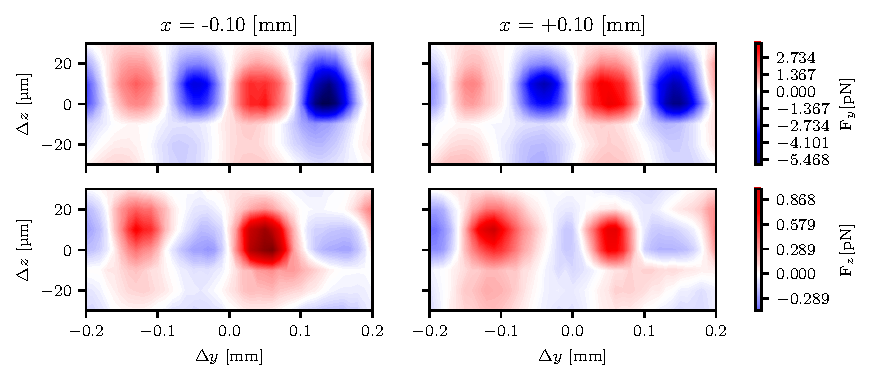
\includegraphics[width=\figWidthDouble]{\relPath/10_Figures/4um.pdf}
  % \input{10_Figures/PGF/4um_map.pgf}
  \caption{Measured steady-state acoustic forces for a \Dfour~particle with 
    $\fex=\SI{4.015}{\MHz}$ and $V_{\text{pp}} = \SI{10.7}{\volt}$. The top row 
    depicts the forces along $\ey$ and the bottom along $\ez$. The two columns 
    correspond to two different measurement $yz$-planes at $x=\SI{-0.1}{\mm}$ 
  and $x=\SI{0.1}{\mm}$, respectively.}\label{fig:4um-map}
\end{figure}

\begin{figure}[H]
  \centering
  % \input{10_Figures/PGF/2um_map.pgf}
  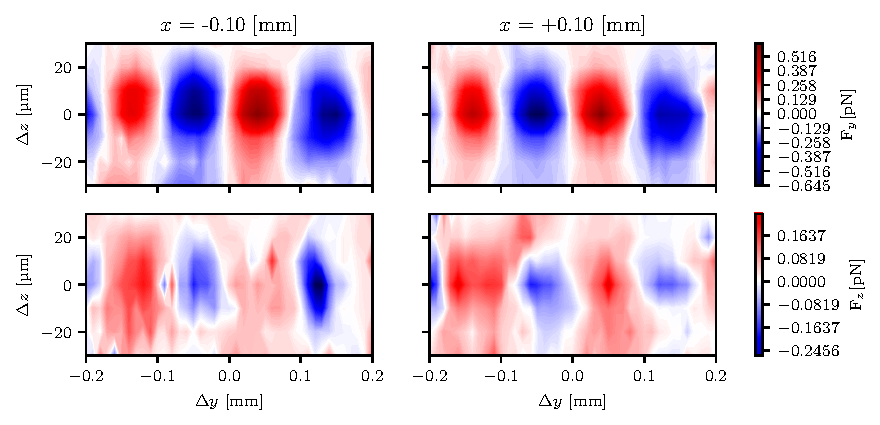
\includegraphics[width=\figWidthDouble]{\relPath/10_Figures/2um.pdf}
  \caption{Measured steady-state acoustic forces for a \Dtwo~particle with 
    $\fex=\SI{4.015}{\MHz}$ and $V_{\text{pp}} = \SI{10.7}{\volt}$. The top row 
    depicts the forces along $\ey$ and the bottom along $\ez$. The two columns 
  correspond to two different measurement $yz$-planes at $x=\SI{-0.1}{\mm}$ and 
$x=\SI{0.1}{\mm}$, respectively.}\label{fig:2um-map}
\end{figure}
\clearpage
}

\subsection{Stationary Force Measurement}
In preparation for the time evolution measurement, where a spatial position of 
orthogonal AS forces and ARFs is beneficial, we characterized our device with 
two sets of stationary force measurements at a constant excitation frequency. 
For those measurements the optical trapping force is greater than the acoustic 
forces. One measurement was with a \Dtwo, and the other with a \Dfour~diameter 
particle. For changing the particle size we needed to empty and refill the 
device.  We kept the ambient conditions and experiment settings between the two 
measurements as constant as possible. For the measurements with the 
\Dtwo~particle the ambient temperature was \SI{24.49}{\celsius} in average with 
a standard deviation of \SI{0.10}{\celsius} and for the measurement with the 
\Dfour~particle the average temperature was \SI{24.78}{\celsius} with a 
standard deviation of \SI{0.25}{\celsius} ensuring the same experimental 
conditions for both measurements. More details regarding the protocol of those 
measurements can be found in \cite{Lamprecht2016} by 
\citeauthor{Lamprecht2016}.

We defined two $yz$ measurement planes, with $x_{1} = \SI{-0.1}{\mm}$ and 
$x_{2} = \SI{0.1}{\mm}$, respectively. In each plane we defined a grid in 
$y_{i} \in \{-0.20,0.19,\dots,0.20\}\, \si{\mm}$ and $z_{j} \in 
\{-30,-20,\dots,30\}\,\si{\um}$. At each point $(y_{i}, z_{j})$ we measured the 
forces in all three dimensions 5 times for \SI{3}{\second} each. Our excitation 
frequency was set to $\fex = \SI{4.015}{\MHz}$ and the applied voltage was 
$U_{\text{pp}} = \SI{10.7}{\volt}$. We choose $\fex$ based on a frequency sweep 
and the corresponding maximal forces in this sweep. With the chosen $\fex$ and 
the fluid speed of sound $\cfl \approx \SI{1500}{\meter\per\second}$, we obtain 
the theoretical acoustic wavelength of $\lap = \sfrac{\cfl}{\fex} \approx 
\SI{375}{\um}$. Hence, with the frequency $\fex$ and a channel width of $W = 
\SI{3}{\mm}$, 16 pressure nodal lines are present. For each spatial position we 
averaged the forces over the \SI{3}{\second} timespan and also over the 5 
repetitions.

\Cref{fig:4um-map,fig:2um-map} visualize stationary force measurement results 
as contour plots for the two particle sizes. In addition, 
\Cref{fig:averaged_forces_vs_dy} depicts the measured forces in $\ey$ and $\ez$ 
directions, when the data is additionally averaged over the 7 different heights 
$\Dz$. For \Cref{subfig:F_y,subfig:F_z}, the left vertical axis is the scale 
for the \Dfour~particle and the right vertical axis for \Dtwo~particles.

In \Cref{subfig:F_y} the force wavelength $\laF$ is estimated to be 
\SI{180}{\um} which is in line with the theoretical wavelength $\laF = 
\sfrac{\lap}{2}$. One can also note that the shape of two force measurements is 
consistent. The ratio of the mean maximal force amplitudes $\frac{1.25}{0.17} = 
7.13$ is about the same as the ratio of the cubed diameter
\begin{equation}
  {\left( \frac{\Dfour}{\Dtwo} \right)}^{3} \approx 2.13^{3} \approx 9.68
 \label{eq:TC-ARF-AS-scaling}
\end{equation}
Based on the theoretical scaling laws we conclude that the forces in the $\ey$ 
direction are ARF dominant.


In \Cref{subfig:F_z} one can see the measured forces in $\ez$ for both particle 
sizes and both measurement $yz$ planes. As for the forces in $\ey$ direction, 
in \Cref{subfig:F_y}, the forces in $\ez$ direction are averaged over all 
$\Dz$. The force magnitude for both sizes is smaller than in $\ey$ direction 
for both particle sizes. The shapes, however, are similar but not as consistent 
as in \Cref{subfig:F_y}. The ratio of the mean maximal force amplitudes 
$\frac{0.25}{0.08} \approx 3.1$ is about the same as the ratio of the two 
diameters, which suggests that in the $\ez$ direction the forces on the 
particle are AS dominated (see \Cref{eq:TC-ARF-AS-scaling}).

\begin{figure}[H]
  \centering
  \begin{subfigure}{\figWidth}
    \centering
    \caption{$F_{y}$ [\si{\pico\newton}]}\label{subfig:F_y}
    % \tikzsetnextfilename{avgF_y_vs_dy}
\begin{tikzpicture}
  \begin{axis}[%
      scale only axis,
      width = 60mm,
      height = 5cm,
      axis y line*=left,
      legend style={
        fill=blue!10!white,
        font=\tiny,
        at={(0.03,0.05)},
        anchor=south west},
      xlabel = {$\Dy$ [\si{\mm}]}]

    \fill[fill=black!15!white] ({axis cs:-0.06,-2}|-{rel axis cs:0,0}) 
    rectangle ({axis cs:-0.03,2}|-{rel axis cs:0,1});

    \addlegendimage{empty legend}
    \addlegendentry{\hspace{-.6cm}\textbf{$\Rfour$}}

    \addplot[thick, blue] table[x=dy, y=F4_y1] 
    {\relPath/10_Figures/TikZ/averaged_yz_Forces.dat};
    \addlegendentry{$x_{1}$};

    \addplot[thick, blue, dashed] table[x=dy, y=F4_y2] 
    {\relPath/10_Figures/TikZ/averaged_yz_Forces.dat};
    \addlegendentry{$x_{2}$};


    \draw[|<->|] ({axis cs:-0.135,0}|-{rel axis cs:0,0.95}) -- ({axis 
    cs:0.05,0}|-{rel axis cs:0,0.95}) node[midway,below] 
    {$\sfrac{\lap}{2}=\laF$};


  \end{axis}
  \pgfplotsset{every axis y label/.append style={rotate=180,yshift=86mm}}
  \begin{axis}[%
      scale only axis,
      width = 60mm,
      height = 5cm,
      legend style={
        fill=lightgray,
        font=\tiny,
        at={(0.97,0.95)},
        anchor=north east},
      axis x line=none,
    axis y line*=right]

    \addlegendimage{empty legend}
    \addlegendentry{\hspace{-.6cm}\textbf{$\Rtwo$}}

    \addplot[thick, dotted] table[x=dy, y=F2_y1] 
    {\relPath/10_Figures/TikZ/averaged_yz_Forces.dat};
    \addlegendentry{$x_{1}$};

    \addplot[thick,loosely dashed] table[x=dy, y=F2_y2] 
    {\relPath/10_Figures/TikZ/averaged_yz_Forces.dat};
    \addlegendentry{$x_{2}$};

  \end{axis}
\end{tikzpicture}

    % \includegraphics[width=\subfigWidth]{Plots/cache/avgF_y_vs_dy.eps}
    \includegraphics[]{Plots/cache/avgF_y_vs_dy.eps}
  \end{subfigure}%
  \begin{subfigure}{\figWidth}
    \centering
    % \tikzsetnextfilename{avgF_z_vs_dy}
\begin{tikzpicture}
  \begin{axis}[%
      scale only axis,
      width = 60mm,
      height = 5cm,
      axis y line*=left,
      legend style={
        fill=blue!10!white,
        font=\tiny,
        at={(0.03,0.05)},
        anchor=south west},
      xlabel = {$\Dy$ [\si{\mm}]}]

    \fill[fill=black!15!white] ({axis cs:-0.06,-2}|-{rel axis cs:0,0}) 
    rectangle ({axis cs:-0.03,2}|-{rel axis cs:0,1});

    \addlegendimage{empty legend}
    \addlegendentry{\hspace{-.6cm}\textbf{$\Rfour$}}

    \addplot[thick,blue] table[x=dy, y=F4_z1] 
    {\relPath/10_Figures/TikZ/averaged_yz_Forces.dat};
    \addlegendentry{$x_{1}$};

    \addplot[thick, blue, dashed] table[x=dy, y=F4_z2] 
    {\relPath/10_Figures/TikZ/averaged_yz_Forces.dat};
    \addlegendentry{$x_{2}$};

  \end{axis}
  \pgfplotsset{every axis y label/.append style={rotate=180,yshift=86mm}}
  \begin{axis}[%
      scale only axis,
      width = 60mm,
      height = 5cm,
    axis y line*=right,
      yticklabel style={
        /pgf/number format/fixed,
        /pgf/number format/precision=2
      },
      legend style={
        fill=lightgray,
        font=\tiny,
        at={(0.97,0.95)},
        anchor=north east},
      axis x line=none]

    \addlegendimage{empty legend}
    \addlegendentry{\hspace{-.6cm}\textbf{$\Rtwo$}}

    \addplot[thick, dotted] table[x=dy, y=F2_z1] 
    {\relPath/10_Figures/TikZ/averaged_yz_Forces.dat};
    \addlegendentry{$x_{1}$};

    \addplot[thick,loosely dashed] table[x=dy, y=F2_z2] 
    {\relPath/10_Figures/TikZ/averaged_yz_Forces.dat};
    \addlegendentry{$x_{2}$};

  \end{axis}
\end{tikzpicture}

    % \includegraphics[width=\subfigWidth]{Plots/cache/avgF_z_vs_dy.eps}
    \caption{$F_{z}$ [\si{\pico\newton}]}\label{subfig:F_z}
    \includegraphics[]{Plots/cache/avgF_z_vs_dy.eps}
  \end{subfigure}%
  \caption{Measured steady-state acoustic forces when averaged over the cavity 
    height. All values are in \si{\pico\newton}. For each plot the left 
    $y$-axis is the measured force on the \Dfour~($D_{4}$) particle and the 
    right one for the \Dtwo~($D_{2}$) particle, respectively.
    The gray shaded area corresponds to the positions where the time evolution 
  is measured.}\label{fig:averaged_forces_vs_dy}
\end{figure}

\subsection{Measurement Protocol for Time Evolution}

Based on a set of proof-of-concept experiments (data not shown here) and the 
information from numerical simulations that the AS field in a \emph{real} 
device can substantially differ from the AS field of fluid cavity-only 
structure, we selected $x = 0$, $y_{i} \in 
\{-0.15,-0.14,\dots,0.10\}\,\si{\mm}$, and $z_{j} \in \{-10,0,10\}\,\si{\um}$. 
This choice means, that we measure at the same $y_{i}$ and $z_{j}$ as for the 
stationary force measurement. We have the same excitation frequency ($\fex = 
\SI{4.015}{\MHz}$) as in the stationary force measurements from before. However 
we set the excitation amplitude slightly higher to $U_{\text{pp}} = 
\SI{11.7}{\volt}$ in order to increase the signal to noise ratio (SNR).

We control the whole measuring routine with a self-written Python program. 
Before each measurement, the offset of the QPDs is checked and, if needed, 
adjusted. First we measure without US and then we measure with US on. We repeat 
this procedure 50 times before moving to the next location.

For the time evolution measurement, we acquire with a sampling rate of $\fs 
=\SI{1.25}{\MHz}$ ($\Dt = \SI{0.8}{\us}$) for \SI{125}{\ms} the three QPD 
signals, the signal for the shutter, and the DC signal for the laser as soon as 
the shutter starts opening ($t = \SI{-25}{\ms}$ in \Cref{fig:daq-sync}). 
Between $t =\SI{0}{\ms}$ and $t = \SI{30}{\ms}$ the shutter is completely open 
and the US is switched on. Extending the measurement time further has no 
benefit because the particle will be outside the linear regimes of the QPDs and 
might move too far from the OT trapping region such that it cannot be 
recaptured after the laser changes to its high power state again.

We repeat 50 times per position because the particle starts sedimenting 
as soon as the laser power drops to the lower value. During this movement the 
particle still undergoes Brownian motion. Hence, the trajectory is not straight 
along the $\ez$ direction. With 50 datasets, we can average this random 
movement out.

Taking the approximation of \cref{eq:TC-mod-free-fall} into account, a \Dtwo~large 
\SiO~sphere sedimenting in water reaches its terminal velocity 
almost instantaneously, because the inertia term is small; additionally, the 
sphere travels about $0.12\,\Rtwo$ in \SI{55}{\ms}. Therefore, after 
\SI{25}{\ms} the particle is still in the linear regime of the QPDz. The static 
gravitational force ($\tilde{m}g$) with the added buoyancy of water is less 
than \SI{40}{\femto\newton} for the \Dtwo~particle. This is more than 6 times 
smaller than the maximal measured force in $\ez$ direction. Therefore, we 
assume in areas of maximal forces along $\ez$ that the driving force of this 
movement is either the acoustic field or $\FAS$. With an ideal sedimentation in 
the first \SI{25}{\ms} along $\ez$, the laser spot on QPDxy does not change at 
all during the sedimentation.

\subsection{Data Processing}

The acquired data is postprocessed with Python. We look at discrete points 
every $t_{k} = k\cdot\SI{0.1}{\ms}$ with $k\in \mathbb{N}$. In addition, we use 
a moving average for the data at $t_{k}$ with a centered window size of 101 
data points, corresponding to a timespan of \SI{80}{\us}. Next, we subtract the 
data series without US from the series with US to obtain the delta voltage 
$\DV_{m}$, with $m$ being $y$ or $z$. This quantity allows us to further reduce 
unwanted noise. This step serves also as data quality check because all 
measurements have the same protocol until $t=\SI{0}{\ms}$. Hence, the delta 
voltage $\DV_{m}$ must be \emph{zero} for $t\leq\SI{0}{\ms}$. Then, we average 
$\DV_{m}$ over the 50 repetitions per spatial position $y_{i}, z_{j}$. As last 
step for the time evolution plots, we normalize the data by the $\max\left( 
\left\vert \DV_{m}(t)\right\vert \right)$ for $\SI{10}{\ms} < t < 
\SI{30}{\ms}$.

\section{Results and Discussion\label{sec:TC-results}}

\Cref{subfig:res_DV_y} shows that the maximal averaged voltage difference 
$\DV_{y}$ for the \Dtwo~particle while having the leaser in the 
$P_{\text{measure}}$ mode. It has the same shape as the stationary force 
measurement in \cref{subfig:F_y}.  However, the smoothness of $\DV_{y}$ is 
worse. We attribute this to the nature of the experiment, as the recorded 
motion of the particle is caused by two effects; one is the acoustic field and 
the other is the always present Brownian motion.  For the stationary force 
measurements the particle is fixed in place by the optical potential and the 
Brownian motion is negligible.

By measuring the same shape with the two experiments, we could validate our 
measurement protocol. As for the stationary measurements, the SNR of the 
evolution measurement and also shape are better for the in-plane $\ey$ than the 
axial $\ez$ (see \cref{subfig:F_y} and \cref{subfig:F_z}). Nevertheless, 
\cref{subfig:F_z} and \cref{subfig:res_DV_z} also show similar shapes. We want 
to stress again, that the amplitudes of \cref{fig:DV_vs_dy} are not comparable 
to each other for $\ey$ and $\ez$ (see \cref{sec:TC-experimental-setup}).
% This step enables data comparability, because the raw magnitudes are 
% inherently different. As stated before, the in-plane position detection along 
% $\ex$ and $\ey$ functions differently than the axial along $\ez$.

The numerical streaming simulations of a fluid cavity with and without the
surrounding structure showed that the streaming field is a local effect in a
model with surrounding structure. In our experiments we saw similar tendencies.  
However, not all measured spatial locations had enough actual signal strength 
to further investigate. In \Cref{fig:evolutioin-V} we plot the time evolution 
of the signal for four different $\Dy$ where it is clear that the signal is due 
to the acoustic field and not to noise or Brownian motion.

\begin{figure}[ht]
  \centering
  \begin{subfigure}{\figWidth}
    \centering
    \caption{Data for $y$-component ($m = y$)}\label{subfig:res_DV_y}
    % \tikzsetnextfilename{avgV_y_vs_dy}
\begin{tikzpicture}
  \begin{axis}[%
      scale only axis,
      width = 60mm,
      height = 45mm,
      xticklabel style={
        /pgf/number format/fixed,
        /pgf/number format/precision=2
      },
      legend style={
        fill=lightgray,
        font=\tiny,
        at={(0.97,0.05)},
        anchor=south east
      },
      legend cell align={left},
      ylabel={$\max\left( \DV_{m}\left( t \right) \right)$ [\si{\mV}]},
      xlabel = {$\Dy$ [\si{\mm}]}]

      \fill[fill=black!15!white] ({axis cs:-0.065,-0.0002}|-{rel axis cs:0,0}) 
      rectangle ({axis cs:-0.025,0.0002}|-{rel axis cs:0,1});

    \addplot[thick,mark=*,mark size=1pt] table[x=dy, y=DV_y_m10] 
    {\relPath/10_Figures/TikZ/averaged_yz_mVoltages.dat};
    \addlegendentry{$\Dz = -10$};

    \addplot[thick, dotted,mark=*,mark size=1pt] table[x=dy, y=DV_y_m00] 
    {\relPath/10_Figures/TikZ/averaged_yz_mVoltages.dat};
    \addlegendentry{$\Dz = 0$};

    \addplot[thick, dashed,mark=*,mark size=1pt] table[x=dy, y=DV_y_p10] 
    {\relPath/10_Figures/TikZ/averaged_yz_mVoltages.dat};
    \addlegendentry{$\Dz = +10$};

    % wavelength
    \draw[|<->|] ({axis cs:-0.135,0}|-{rel axis cs:0,0.55}) -- ({axis 
    cs:0.05,0}|-{rel axis cs:0,0.55}) node[midway,above] 
    {$\sfrac{\lap}{2}=\laF$};

  \end{axis}
\end{tikzpicture}

    \includegraphics[]{Plots/cache/avgV_y_vs_dy.eps}
  \end{subfigure}%
  \begin{subfigure}{\figWidth}
    \centering
    \caption{Data for $z$-component ($m = z$)}\label{subfig:res_DV_z}
    % \tikzsetnextfilename{avgV_z_vs_dy}
\begin{tikzpicture}
  \begin{axis}[%
      scale only axis,
      width = 60mm,
      height = 45mm,
      xticklabel style={
        /pgf/number format/fixed,
        /pgf/number format/precision=2
      },
      legend style={
        fill=lightgray,
        font=\tiny,
        at={(0.97,0.05)},
        anchor=south east
      },
      legend cell align={left},
      xlabel = {$\Dy$ [\si{\mm}]}]

      \fill[fill=black!15!white] ({axis cs:-0.065,-0.0002}|-{rel axis cs:0,0}) 
      rectangle ({axis cs:-0.025,0.0002}|-{rel axis cs:0,1});

    \addplot[thick,mark=*,mark size=1pt] table[x=dy, y=DV_z_m10] 
    {\relPath/10_Figures/TikZ/averaged_yz_mVoltages.dat};
    \addlegendentry{$\Dz = -10$};

    \addplot[thick, dotted,mark=*,mark size=1pt] table[x=dy, y=DV_z_m00] 
    {\relPath/10_Figures/TikZ/averaged_yz_mVoltages.dat};
    \addlegendentry{$\Dz = 0$};

    \addplot[thick, dashed,mark=*,mark size=1pt] table[x=dy, y=DV_z_p10] 
    {\relPath/10_Figures/TikZ/averaged_yz_mVoltages.dat};
    \addlegendentry{$\Dz = +10$};

  \end{axis}
\end{tikzpicture}

    \includegraphics[]{Plots/cache/avgV_z_vs_dy.eps}
  \end{subfigure}%
  \caption{Maximal $\DV_{y}$ and $\DV_{z}$ averaged over all repetitions in the 
    timespan between \SI{35}{\ms} and \SI{55}{\ms} for the three different 
    measurement heights $\Dz = \SIlist[list-units=single, list-final-separator 
    = {, }, list-pair-separator= {, }] {-10;0;10}{\um}$. The gray shaded area 
    represents the $\Dy_{i}$ of best signal strength for $\max\left( 
    \DV_{z}\left( t \right) \right)$. The data points of best strength are 
    taken for the time evolution results. The wavelength marker represents the 
  same length as in \cref{subfig:F_y}.}\label{fig:DV_vs_dy}
\end{figure}%

Since we show $\DV_{m}$ rather than the absolute voltage amplitudes, we can 
further validate our protocol. For $\sfrac{t}{t_{0}} < 0$, where $t_{0} = 
\sfrac{1}{\fex}$ and $\sfrac{t}{t_{0}}=0$ represents the time when the US is 
switched on (in \cref{fig:daq-sync} $t = \SI{0}{\ms}$), all data series in 
\cref{fig:evolutioin-V} are zero. All data series for $\ez$ are more noisy than 
for $\ey$. However, we also have the same amplitude of noise in $\ey$ 
direction. But, the normalization value for the data series for $\ey$ is 
inherently larger than for $\ez$ (see \cref{fig:DV_vs_dy}).

\afterpage{
\begin{figure}[ht]
  \centering
  % \tikzsetnextfilename{evolution_V}
%%%%%%%
% READ TABLE
%%%%%%%
\pgfplotstableread{\relPath/10_Figures/TikZ/evolution_yz_Voltages.dat}{\data}
%%%%%%%
% LINES FOR ALL GROUPPLOTS
%%%%%%%
\renewcommand{\tikzHelper}{
  \fill[fill=black!10!white] (axis cs:-80,0) rectangle (axis cs:0,1);

  \draw[dotted] (axis cs:0,0) -- (axis cs:0,1);
  \draw[dotted] (axis cs:50,0) -- (axis cs:50,1);
  \draw[dotted] (axis cs:100,0) -- (axis cs:100,1);
  \draw[dotted] (axis cs:-80,0.5) -- (axis cs:120,0.5);
  \draw[dotted] (axis cs:-80,0.5) -- (axis cs:120,0.5);
}



\begin{tikzpicture}
   \begin{groupplot}[%
       scale only axis,
       group style={
         group size= 2 by 4,
         group name=plots,
         vertical sep=4pt,%
         horizontal sep=8pt},%
       height=40mm,%
       width=64mm,%
        xticklabel style={
          /pgf/number format/fixed,
          /pgf/number format/precision=2
        }]

%%%%%%
%%% PLOT (1,1)
%%%%%%

   \nextgroupplot[%
      legend style={
        fill=lightgray,
        font=\tiny,
        at={(0.03,0.95)},
        anchor=north west
      },
      legend cell align={left},
     xticklabels={,,},
     % title={$\DV_{y}\,|\,\Dy = \SI{-0.06}{\milli\meter}$},%
     title={Data for $y$-component ($m = y$)},%
     ylabel={$\sfrac{\DV_{m}}{\DV_{m,\text{max}}}$}]

      \tikzHelper
      \draw[thick,|<->|] (axis cs:-80,0.25) -- (axis cs:0,0.25) node[midway, 
      above] {US off};

      \addplot[thick] table[x=dt, y=DV_y_m06_m10] {\data};

      \addplot[thick, dotted] table[x=dt, y=DV_y_m06_m00] {\data};

      \addplot[thick, dashed] table[x=dt, y=DV_y_m06_p10] {\data};

      \addlegendentry{$\Dz = \SI{-10}{\um}$};
      \addlegendentry{$\Dz = \SI{0}{\um}$};
      \addlegendentry{$\Dz = \SI{+10}{\um}$};



%%%%%%
%%% PLOT (1,2)
%%%%%%

   \nextgroupplot[%
     xticklabels={,,},
     yticklabels={,,},
     title={Data for $z$-component ($m = z$)}]%
   % title={$\DV_{z}\,|\,\Dy = \SI{-0.06}{\milli\meter}$}]

      \tikzHelper

      \addplot[thick] table[x=dt, y=DV_z_m06_m10] {\data};

      \addplot[thick, dotted] table[x=dt, y=DV_z_m06_m00] {\data};

      \addplot[thick, dashed] table[x=dt, y=DV_z_m06_p10] {\data};

%%%%%%
%%% PLOT (2,1)
%%%%%%

   \nextgroupplot[%
     xticklabels={,,},
     ylabel={$\sfrac{\DV_{m}}{\DV_{m,\text{max}}}$ },
     % title={$\Dy = \SI{-0.05}{\milli\meter}$}
   ]

      \tikzHelper

      \addplot[thick] table[x=dt, y=DV_y_m05_m10] {\data};

      \addplot[thick, dotted] table[x=dt, y=DV_y_m05_m00] {\data};

      \addplot[thick, dashed] table[x=dt, y=DV_y_m05_p10] {\data};

%%%%%%
%%% PLOT (2,2)
%%%%%%

   \nextgroupplot[%
     xticklabels={,,},
     yticklabels={,,},
     % title={$\Dy = \SI{-0.05}{\milli\meter}$}
   ]

      \tikzHelper

      \addplot[thick] table[x=dt, y=DV_z_m05_m10] {\data};

      \addplot[thick, dotted] table[x=dt, y=DV_z_m05_m00] {\data};

      \addplot[thick, dashed] table[x=dt, y=DV_z_m05_p10] {\data};

%%%%%%
%%% PLOT (3,1)
%%%%%%

   \nextgroupplot[%
     xticklabels={,,},
     ylabel={$\sfrac{\DV_{m}}{\DV_{m,\text{max}}}$ },
     % title={$\Dy = \SI{-0.04}{\milli\meter}$}
   ]

      \tikzHelper

      \addplot[thick] table[x=dt, y=DV_y_m04_m10] {\data};

      \addplot[thick, dotted] table[x=dt, y=DV_y_m04_m00] {\data};

      \addplot[thick, dashed] table[x=dt, y=DV_y_m04_p10] {\data};

%%%%%%
%%% PLOT (3,2)
%%%%%%

   \nextgroupplot[%
     xticklabels={,,},
     yticklabels={,,},
     % title={$\Dy = \SI{-0.04}{\milli\meter}$}
   ]

      \tikzHelper

      \addplot[thick] table[x=dt, y=DV_z_m04_m10] {\data};

      \addplot[thick, dotted] table[x=dt, y=DV_z_m04_m00] {\data};

      \addplot[thick, dashed] table[x=dt, y=DV_z_m04_p10] {\data};


%%%%%%
%%% PLOT (4,1)
%%%%%%

   \nextgroupplot[%
     ylabel={$\sfrac{\DV_{m}}{\DV_{m,\text{max}}}$},
     xlabel={$10^{3}\,\sfrac{t}{t_{0}}$ },
     % title={$\Dy = \SI{-0.03}{\milli\meter}$}
   ]

      \tikzHelper

      \addplot[thick] table[x=dt, y=DV_y_m03_m10] {\data};

      \addplot[thick, dotted] table[x=dt, y=DV_y_m03_m00] {\data};

      \addplot[thick, dashed] table[x=dt, y=DV_y_m03_p10] {\data};

%%%%%%
%%% PLOT (4,2)
%%%%%%

   \nextgroupplot[%
     yticklabels={,,},
     xlabel={$10^{3}\,\sfrac{t}{t_{0}}$},
     % title={$\Dy = \SI{-0.03}{\milli\meter}$}
   ]

      \tikzHelper

      \addplot[thick] table[x=dt, y=DV_z_m03_m10] {\data};

      \addplot[thick, dotted] table[x=dt, y=DV_z_m03_m00] {\data};

  \end{groupplot}

%%%%%%
%%% TEXT NEXT TO PLOTS
%%%%%%
  \node[rotate=90] at (plots c2r1.east) [yshift=-5mm] {$\Dy = 
  \SI{-0.06}{\milli\meter}$};
  \node[rotate=90] at (plots c2r2.east) [yshift=-5mm] {$\Dy = 
  \SI{-0.05}{\milli\meter}$};
  \node[rotate=90] at (plots c2r3.east) [yshift=-5mm] {$\Dy = 
  \SI{-0.04}{\milli\meter}$};
  \node[rotate=90] at (plots c2r4.east) [yshift=-5mm] {$\Dy = 
  \SI{-0.03}{\milli\meter}$};

\end{tikzpicture}

  \includegraphics[]{Plots/cache/evolution_V.eps}
  \caption{Time evolution of the normalized $\DV_{y}$ (left column) and 
    $\DV_{z}$ (right column) for the three measurement heights $\Dz = 
    \SIlist[list-units=single, list-final-separator = {, }, 
    list-pair-separator= {, }] {-10;0;10}{\um}$ and the positions for $\Dy = 
    \SIlist[list-units=single, list-final-separator = {, }, 
    list-pair-separator= {, }] {-0.06;-0.05;-0.04;-0.03}{\mm}$. The gray shaded 
    area of each plot marks the time when the US is off; 
  $t_{0}=\sfrac{1}{\fex}$.}\label{fig:evolutioin-V}
\end{figure}
}

For all 12 positions $(y_{i}, z_{j})$ in \cref{fig:evolutioin-V} the signal 
along $\ey$ starts changing as soon as the US is switched on. This 
is in line with the estimation of \cref{eq:TC-tau-arf} for $\tarf$. For all data 
series $m = z$ it takes significantly more time until the movement with 
constant velocity starts. To further compare the results, we take as criteria 
the period $p^{\ast} = \sfrac{t^{\ast}}{t_{0}}$, when the normalized $\DV_{m} 
\ge 0.5$ is reached. In \cref{tab:TC-results}, the absolute periods for this 
criteria and the offset between the movement along $\ey$ ($m=z$) and the 
movement along $\ez$ ($m=y$) are shown. Taking a different criteria value 
(e.g., the normalized $\DV_{m} \ge 0.3$) changes the absolute magnitude of the 
values $p^{\ast}$, however the offset does not change significantly. The 
average for all $\Delta p^{\ast}$ is about 17'500 which equates to $\approx 
\SI{4.35}{\ms}$ for the excitation frequency $\fex = \SI{4.015}{\MHz}$.

\begin{table*}
  \centering
  \begin{tabular}{ll *{4}{x{27mm}}}
    \toprule
    \toprule
  {\bfseries $\Dy$} & [\si{\mm}] & -0.06 & -0.05 & -0.04 & -0.03 \\

    \midrule
    % {\small
  {\bfseries $p^{\ast}_{y}$ } & ($\times 1000$) [-] & 64.2, 69.5, 70.7 & 65.8, 
  70.3, 70.3 & 65.8, 60.6, 76.7 & 73.5, 57.4, 74.3 \\[2mm]

  {\bfseries $p^{\ast}_{z}$} & ($\times 1000$) [-] & 80.7, 87.9 88.3 & 86.3, 
  85.5, 86.7 & 83.1, 89.5, 87.5 & 87.9, 86.7,  \\

    \midrule
    
  {\bfseries $\Delta p^{\ast}$} & ($\times 1000$) [-] & 16.5, 18.4, 17.6 & 
  20.5, 15.2, 16.4 & 17.3, 18.9, 10.8 & 14.4, 29.3, \\
    % }
    \bottomrule
    \bottomrule
    
  \end{tabular}
  \caption{Absolute periods $p^{\ast}_{m}$ when the normalized $\DV_{m} > 0.5$.  
    The three values per column correspond to the three heights $\Dz = 
    \SIlist[list-units=single, list-final-separator = {, }, 
    list-pair-separator= {, }] {-10;0;10}{\um}$ per $\Dy$ respectively. For 
  $\Dy = \SI{-0.03}{\mm}$ and $\Dz = \SI{10}{\um}$ no data is available for 
$p_{z}^{\ast}$. The last row states the offset $\Delta p^{\ast} = p^{\ast}_{z} 
- p^{\ast}_{y}$}\label{tab:TC-results}
\end{table*}

In addition, all slopes for the $y$ movement ($m=y$) are linear almost 
immediately after the US is
switched on. This suggests, that the ARF is constant and accelerates the 
particle fast to its terminal velocity. The measured voltages and also their 
differences are linearly related to the traveled distances. Hence, a constant 
increase in voltage, which means a constant voltage increase per time 
$\sfrac{\text{d}\,\DV_{m}}{\text{d}t} = const.$, implies a constant particle 
speed along the $\ey$ direction. The particle trajectory in $\ez$ direction is 
predominantly affected by the streaming field. This fluid motion takes more 
time until it is established. With the same reasoning as before, a linear slope 
for the $z$ movement ($m=z$) in \cref{fig:evolutioin-V} implies a constant 
force and constant particle speed. A constant speed means a non-changing 
streaming field and therefore a constant streaming velocity.


\section{Conclusion\label{sec:conclusion}}

In this work we presented the measurement of the temporal evolution of the AS 
field and the ARF in a BAW device utilizing an OT. We slightly modified our 
validated optical trapping setup \cite{Lamprecht2016,Lamprecht2021} to 
accommodate the requirements of this experiment. With a temporal resolution of 
$\Dt=\SI{0.8}{\us}$ we could measure at least every fourth time period of 
excitation. We validated our measurement protocol against the stationary force 
field.

We monitored the trajectory of a \Dtwo~\SiO~particle as soon as the US 
excitation of the device started. We selected measurement positions in a 
standing pressure wave mode where ARF dominates in one direction and AS 
orthogonal to it. In addition, we chose the spatial location within the mode 
to maximize the amplitude of both effects. Our measurements show, that the ARF 
is established almost immediately after the US is switched on; whereas the AS 
takes in average 17'500 excitation periods (\SI{4.4}{\ms}) longer to evolve. 
This time is about four times larger than the theoretical approximation with 
the momentum diffusion time.

These results show that the build up of AS takes significantly longer than the 
build up of the ARF. This temporal difference can explain why a pulsed acoustic 
excitation can prevent streaming as it has been experimentally shown by 
\citeauthor{Hoyos2013} \cite{Hoyos2013,Castro2016}. In addition, the results of 
the streaming simulations of a cavity-only model and a whole-device model show 
that simplified models are enough for simulations of the pressure fields, 
however they cannot reflect \emph{real} streaming patterns. This insight might 
also explain why \citeauthor{Muller2015} could not reproduce the suppression of 
AS with a pulsed excitation in their cavity-only model.



\cleardoublepage
\renewcommand{\relPath}{SECTION/40_Pulsing/}

\chapter[Pulsed Build up Measurement]{Measuring the effects of a pulsed 
  excitation on the build up of acoustic streaming and the acoustic radiation 
  force utilizing an optical tweezer
}\label{ch:pulsing}
\textit{This chapter is original work by Christoph Goering:
\footnote{: DOI: 10.1103/PhysRevE.104.025104, reproduced under the terms of the 
Creative Commons Attribution 4.0 license.}}

\vspace{5mm} \noindent
C. Goering and J. Dual, "Dynamic measurement of the acoustic streaming time 
constant utilizing an optical tweezer", Physical Review E, 2021, \textbf{104}, 
025104.


\section{Abstract}

Pulsed excitations of piezoelectric transducers affect during the build up the 
force contributions from acoustic streaming (AS) and the acoustic radiation 
force (ARF) to the total force in a standing pressure wave differently. We find 
with an optical tweezer as measuring instrument that during the first 120'000 
excitation periods and across different pulsing frequencies, the AS induced 
displacement is in average less than 20\% of its non-pulsed value for a duty 
cycle of 50\%, whereas the ARF induced displacement is around 50\%. These 
findings show that a pulsed excitation can be a tool for reducing AS compared 
to the ARF.
%%%%%%%%%%%%%%%%%%%%%%%%%%%%%%%%%%%%%%%%%%%%%%%%%%%%%%%%%%%%%%%%%%%%%%%%%%%%%%
\section{Introduction}

In acoustofluidic devices two main forces lead to a displacement of an immersed 
object within a pressure wave field: the drag force from acoustic streaming 
(AS) and the acoustic radiation force (ARF). AS typically arises due to viscous 
losses. These viscous losses can appear in the fluid itself (Eckart type 
streaming) \cite{Eckart1948} or in a viscous boundary layer. This boundary 
layer can either be at the interface between the fluid cavity and the 
surrounding medium (Schlichting and Rayleigh streaming) 
\cite{Nyborg1965,Schlichting1932} or even around the object itself 
(microstreaming) \cite{Baasch2019}. Apart from microstreaming, the occurrence 
of AS is independent of the immersed object properties.

The other main force is the ARF. As AS, it is a second order time-averaged 
effect and appears due to scattering of the acoustic incident field at the 
object surface \cite{Yosioka1955,Bruus2012,Gorkov1962}. In contrast to AS, the 
ARF depends also on the ratios of the object and fluid material. For example, 
an object of any material but with an acoustic contrast factor $\Phi$ 
\cite{Bruus2012} of zero magnitude is not displaced due to the ARF because the 
ARF scales linearly with $\Phi$. However, this object will be displaced by the 
drag force arising from AS for any value of $\Phi$.

Besides the material influence, another important difference is the scaling 
with the object dimension for the limit of small particles compared to the 
acoustic wavelength \cite{Bruus2012,King1934}. On the one hand, the drag force 
from AS scales for a spherical object with the radius ($\FAS\propto \R$), and 
on the other hand, the ARF scales with the object volume ($\FARF\propto 
\R^{3}$) \cite{Bruus2012}. At the critical radius ($\R=\Rcrit$) both forces are 
equal in magnitude ($\FARF=\FAS$). For a radius smaller than the critical 
radius ($\R<\Rcrit$) \cite{Bruus2012,Barnkob2012} the drag force from AS 
dominates over the ARF and vice-versa. The forces from AS can be neglected if 
$\R\gg\Rcrit$.

In many acoustofluidic applications the drag forces from AS are undesired 
because they can counteract the ARF \cite{VanAssche2020,Antfolk2014} and hinder 
the application's desired function, e.g. the trapping or focusing of particles. 
Therefore, different techniques for the suppression of AS have been 
investigated in recent years. Hoyos and Castro applied a pulsed excitation to 
the piezoelectric transducer (PZT) leading to a reduction of the steady-state 
streaming flow of up to 50\% compared to the unpulsed flow 
\cite{Hoyos2013,Castro2016}. \cname{Karlsen2018a} utilized in simulations and 
experiments inhomogeneities of the density and of the compressibility within 
the fluid to reduce AS. \cname{Bach2020} optimized the shape of channels with 
numerical simulations to reduce AS by two orders of magnitudes while retaining 
the same level of acoustic pressure. The same AS suppression magnitude was 
achieved by \cname{Winckelmann2021}. They investigated analytically and 
numerically the usage of acoustic electroosmosis to suppress AS.

The combination of optical tweezer (OT) and the acoustic trap is relatively new 
and rare. To the best of the authors' knowledge, \cname{Thalhammer2011} were 
\citeyear{Thalhammer2011} the first to combine these two kind of traps to 
measure the acoustic forces with the OT. In 2014, \cname{Bassindale2014} 
utilized an holographic OT to measure acoustic forces in three dimensions, and 
\cname{Fury2014} used the fine spatial optical resolution and the wide range of 
acoustic trapping for spatially precise manipulation of microbubbles. In 2015 
and 2016, \cname{Lakaemper2015} and \cname{Lamprecht2016} used our single beam 
optical trap to measure the acoustic forces in two and tree dimensions on 
silica micro particles. In 2016, \cname{Thalhammer2016} also combined a 
holographic OT with an acoustic trap to measure the force for excitation 
frequencies above \SI{20}{\mega\hertz}. Lastly in 2021, \cname{Lamprecht2021} 
used our setup to measure the resulting final rotational velocity on 
microparticles due to the acoustic viscous torque.

In 2021, we~\cite{Goering2021} used an OT setup to measure for the first time 
the build up of the ARF and AS on a single spherical particle in a precisely 
characterized \si{\mega\hertz} pressure field. We found that the build up of AS 
is much slower than the build up of the ARF. Our measurements of the AS build 
up revealed approximately 4 times longer build up of AS than the theoretical 
prediction from the momentum diffusion time approximation 
\cite{Muller2015,Goering2021}. Those experimental results indicated that the 
longer-than-expected build up of the AS might be the reason for the pulsed 
excitation to successfully suppress the AS \cite{Hoyos2013,Castro2016}.



Here, we use our measurement routine, the OT setup, the acoustofluidic bulk 
acoustic wave device, and the same acoustic excitation frequency from 
\cite{Goering2021} to dynamically measure the build up of the ARF and AS for a 
acoustic excitation with various pulsing parameter settings.

%%%%%%%%%%%%%%%%%%%%%%%%%%%%%%%%%%%%%%%%%%%%%%%%%%%%%%%%%%%%%%%%%%%%%%%%%%%%%%
%%%%%%%%%%%%%%%%%%%%%%%%%%%%%%%%%%%%%%%%%%%%%%%%%%%%%%%%%%%%%%%%%%%%%%%%%%%%%%
\section{Measurement Protocol}

\begin{figure}[tbp]
  \centering
  % \tikzsetnextfilename{PU-device}
{
\tiny

\begin{tikzpicture}
  % lens
  \definecolor{tempcolor}{RGB}{222, 201, 84}
  \draw[color=white,fill=tempcolor] (0,0.5) circle (0.8);

  % R = (0.2^2+0.4^2)/2/0.2 = 0.5
  % alpha = arcsin(0.4/R) ~53 deg
  \definecolor{tempcolor}{RGB}{176, 206, 255}
  \filldraw[color=black, fill=tempcolor, ultra thin] (-0.4,1) arc 
  (217:323:0.5);

  \draw[fill=white] (-0.5,1) rectangle ++(1,2);

  % PZT
  \filldraw[black,pattern=north west lines] (-3.5,0.7) rectangle ++(0.7,0.2);

  % SI
  \filldraw[black] (-3,-0.5) rectangle ++(-0.5,1);
  \filldraw[black] (+3,-0.5) rectangle ++(+0.5,1);

  % Glas
  \filldraw[color=black, fill=black!15, ultra thin] (-3.5,0.5) rectangle 
  ++(7,0.2);
  \filldraw[color=black, fill=black!15, ultra thin] (-3.5,-0.5) rectangle 
  ++(7,-0.4);

  \draw[|<->|] (-3.5, -1.1) -- node[pos=0.18, below] {\SI{26}{\mm} 
  ($L=\SI{76}{\mm}$)} ++(7,0);

  % cavity
  \filldraw[color=black, fill=blue!20, ultra thin] (-3,-0.5) rectangle ++(6,1);
  \draw[|<->|] (-3, -0.6) -- node[pos=0.2, below] {\SI{3}{\mm}} ++(6,0);
  \draw[|<->|] (-2.8, -0.5) -- node[pos=0.15, right] {\SI{0.1}{\mm}} ++(0,1);

  %pressure field
  \draw[white, variable=\x, domain=-3:3, samples=500] (-1,0) plot 
  (\x,{cos(\x*pi r*3)/4});
  \draw[white, variable=\x, domain=-3:3, samples=500] (-1,0) plot 
  (\x,{-cos(\x*pi r*3)/4});
  % \node at (-2,0.4) {\textcolor{white}{$p_{\mathrm{a}}$}};

  % coordinate system
  \draw[->] (0,0) -- node[pos=1, right] {$\bm{e}_{y}$} ++(0.7,0);
  \draw[->] (0,0) -- node[pos=1, above] {$\bm{e}_{z}$} ++(0,1.7);

  % particle
  \shade[ball color=black!5] (0,0) circle (0.2);

  % condensor
  \filldraw[tempcolor] (0,-1.5) ellipse (1.4 and 0.2);

  % laser
  % \draw[red] (0.35,3.1) -- (0.35,0.92) -- (0,0);
  \draw[red] (0.35,3.1) -- (0.35,0.92) -- (-0.57,-1.5) -- ++(0,-0.3);
  \draw[red] (-0.35,3.1) -- (-0.35,0.92) -- (0.57,-1.5) -- ++(0,-0.3);

  % annotations
  \node[above, align=right, text width=35mm] at (-2.5, 0.9) {PZT 
  (\SI[product-units = single]{4 x 0.5 x 20}{\mm})};
  \node[right] at (1.4, 0.35) {Cavity};
  \node[right] at (1.4, -1.5) {Condensor lens};

  \draw[ultra thin] (0.55, 0.8) -- node[pos=1, right] {Immmersion layer} 
  (1.4,0.9);

  \draw[ultra thin] (0.2, 0.9) -- node[pos=1, right] {Focussing lens} 
  (1.4,1.3);


\end{tikzpicture}
}

  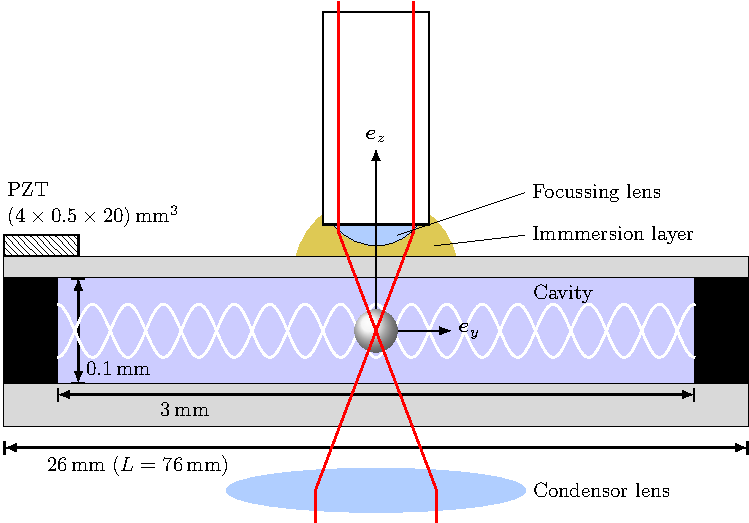
\includegraphics[]{External/PU-device.pdf}
  \caption{Schematic of device and build up measurement 
  setup.}\label{fig:PU-device}
\end{figure}

\begin{figure}[tbp]
  \centering
  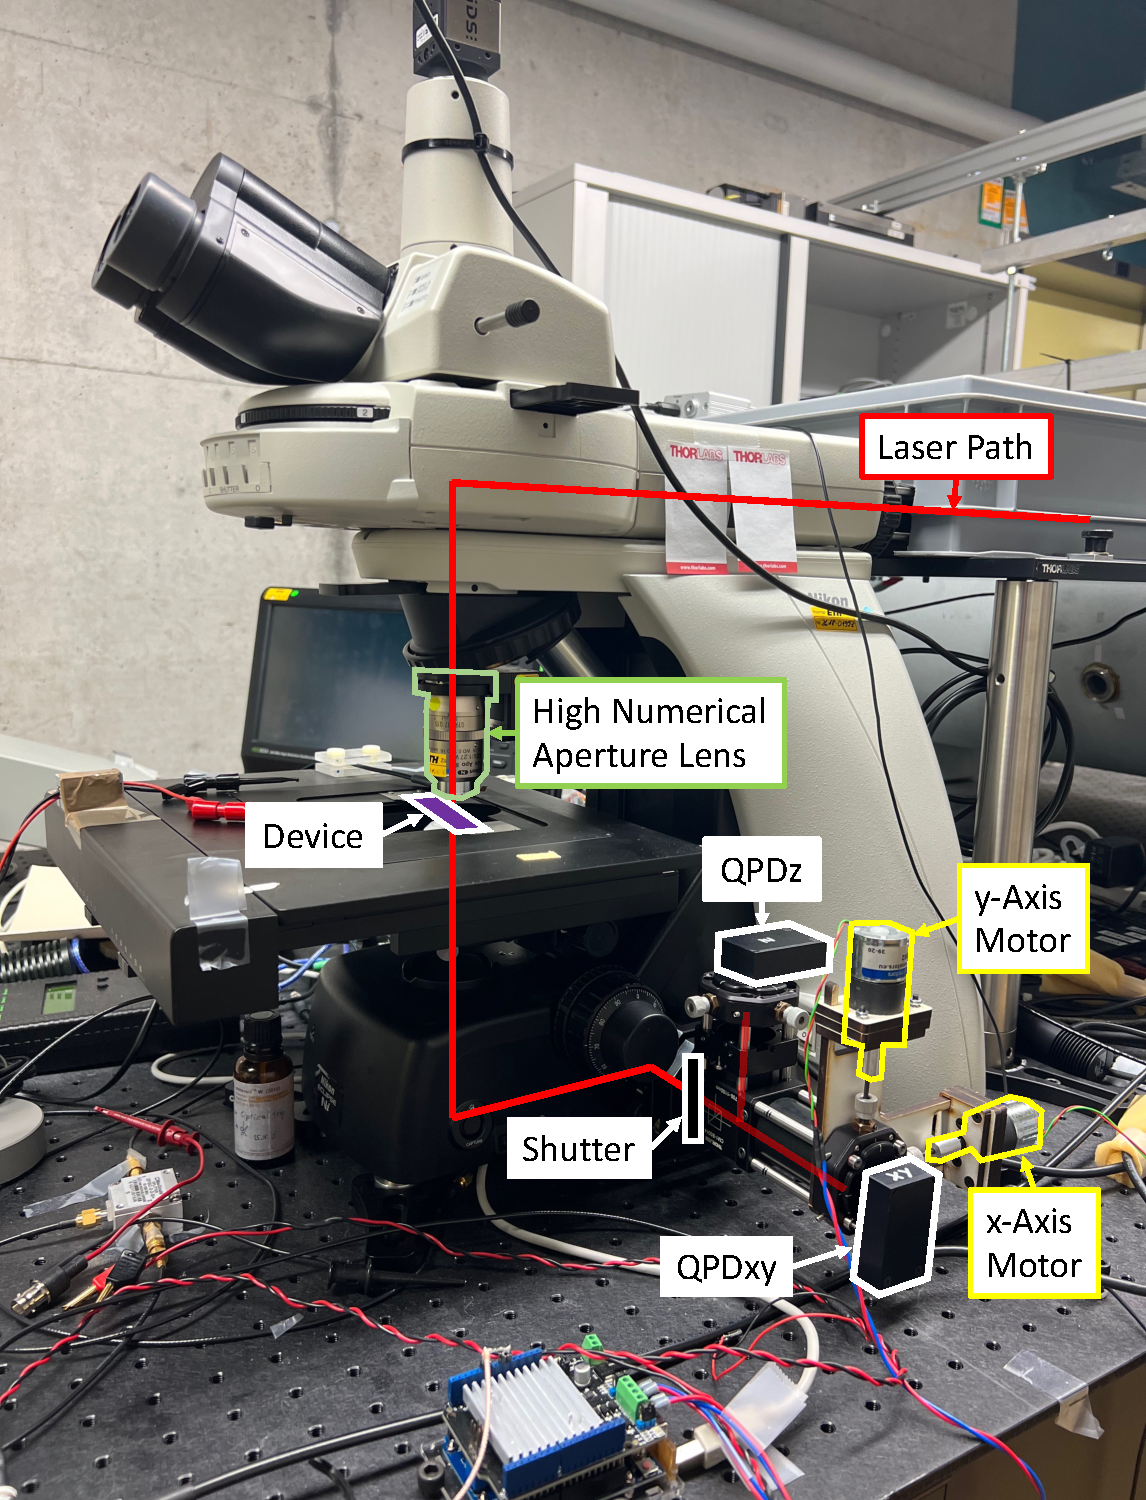
\includegraphics[width=140mm]{Supplemental_OT.pdf}
  \caption{Photograph of optical trapping setup with highlighted important 
  equipment.\label{fig:PU-app-OT}}
\end{figure}

\begin{figure}[tbp]
  \centering
  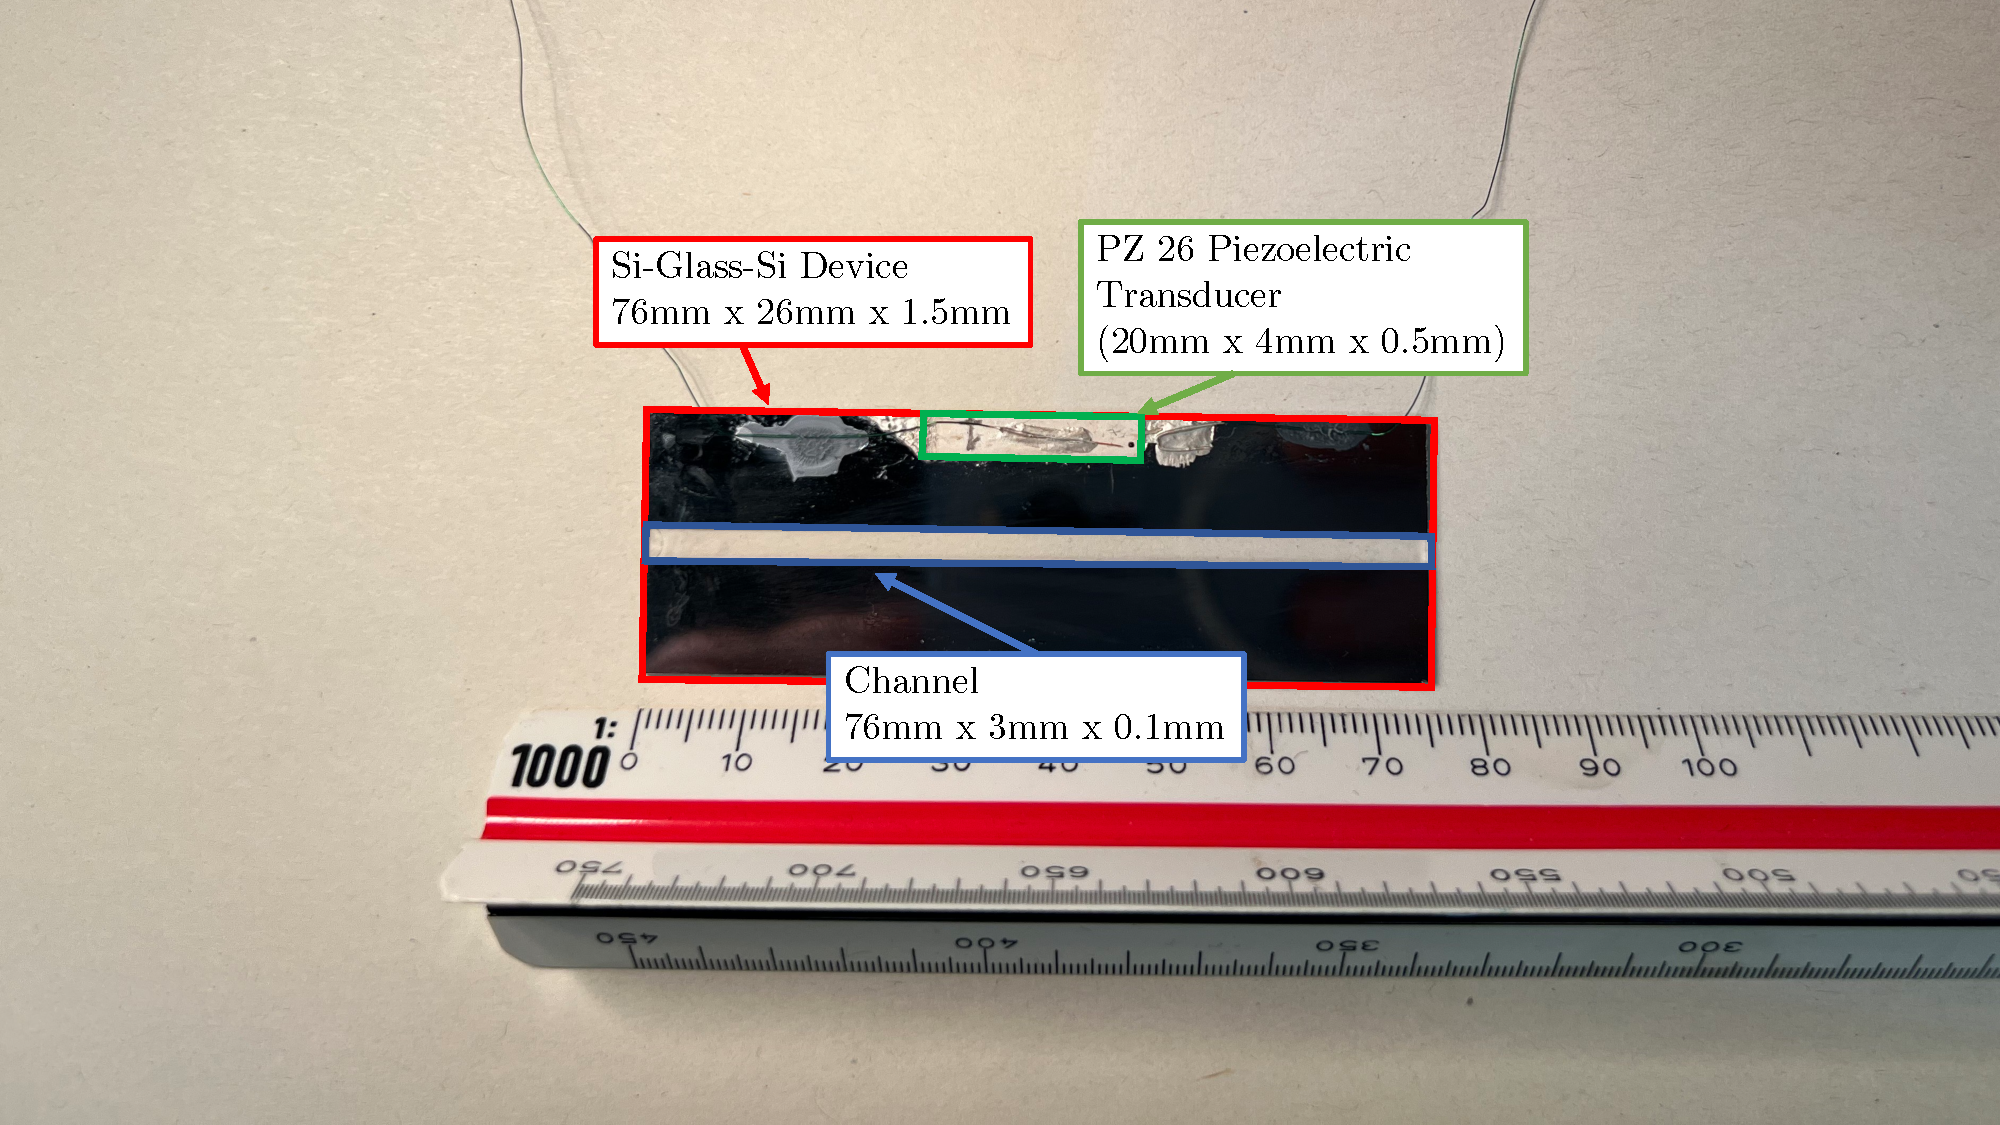
\includegraphics[width=100mm,trim=90mm 45mm 80mm 35mm, clip 
  ]{Supplemental_Device.pdf}
  \caption{Photograph of acoustofluidic device with highlighted parts. 
  \label{fig:PU-app-device}}
\end{figure}

We will highlight the main points of the measurement protocol for the build up 
measurements (BM). A more extensive explanation of each step can be found in 
\citeauthor{Goering2021} \cite{Goering2021}. We can measure with the OT the 
build up of the ARF and AS separately because we determined our BM locations 
such that those two effects are orthogonal to each other; i.e., the ARF points 
in the direction of our $y$ coordinate and the AS points along $z$ (see 
\cref{fig:PU-device}). Our setup (see 
\cref{fig:PU-protocol,fig:PU-app-OT,fig:PU-app-device}) has in its back focal plane two 
quadrant photo detectors (QPDs) for detecting the movement in each spatial 
direction separately 
\cite{Lakaemper2015,Goering2021,Lamprecht2021,Lamprecht2016}. One QPD measures 
the information of the $x$ and $y$ coordinate and the other QPD measures the 
$z$ information. Hence, the build up information of the ARF and AS are also 
separated in the data.

\begin{figure*}[tbp]
  \centering
  % \tikzsetnextfilename{PU-protocol}
{
  \tiny
  \definecolor{tempcolor}{RGB}{176, 206, 255}
\begin{tikzpicture}

% close shutter
\def\y{0}
\pgfmathsetmacro{\ybottom}{\y-0.25)}
\pgfmathsetmacro{\ytop}{\y+0.25)}
\pgfmathsetmacro{\yshutter}{\y-0.5)}
\pgfmathsetmacro{\yshuttert}{\y+0.5)}
\pgfmathsetmacro{\qpd}{\y-0.4)}
\pgfmathsetmacro{\tlaser}{\y+0.2)}
\pgfmathsetmacro{\blaser}{\y-0.2)}
\pgfmathsetmacro{\power}{\y+1.2)}

  \draw[black] (0,\ybottom) rectangle ++(1,0.5);
  \path (0,\ytop) -- ++(1,0) node[above, midway, anchor=south] {Laser};

  \fill[tempcolor] (2.5,\y) ellipse (0.15 and 0.75);
  \path (2,0.75) -- ++(1,0) node[above, midway, anchor=south] {Focussing lens};

  \shade[ball color=black!10] (3.5,\y) circle (.25);

  \path (3.25,\ytop) -- ++(0.5,0) node[above, midway] {particle};
  \path (3.25,\ybottom) -- ++(0.5,0) node[below, midway] {trapped};

  \fill[tempcolor] (4.5,\y) ellipse (0.15 and 0.75);
  \path (4,0.75) -- ++(1,0) node[above, midway, anchor=south] {Condensor lens};

  \filldraw[color=black, fill=black!50] (5.5,\yshutter) rectangle ++(1,1);
  \path (5.5,\yshuttert) -- ++(1,0) node[above, midway, anchor=south] 
  {shutter};
  \path (5.5,\y) -- ++(1,0) node[midway] {$T< 1\%$};
  \path (5.5,\yshutter) -- ++(1,0) node[below, midway] {closed};

  \fill[tempcolor] (7.5,\y) ellipse (0.15 and 0.75);
  \path (7,0.75) -- ++(1,0) node[above, midway, anchor=south] {lens 3};

  \filldraw[color=black, fill=black!10] (9,\qpd) rectangle ++(0.8,0.8);
  \path (9,0.5) -- ++(0.8,0) node[above, midway, anchor=south] {QPDs};
  \filldraw[color=red!50] (9.4,\y) circle (.2);

  \draw[dotted, black] (9, \y) -- ++(0.8,0);
  \draw[dotted, black] (9.4, \qpd) -- ++(0,0.8);

  \draw[red, thick] (1,\blaser) -- ++(1.5,0) -- ++(2,0.4) -- (5.5,\tlaser);
  \draw[red, thick] (1,\tlaser) -- ++(1.5,0) -- ++(2,-0.4) -- (5.5,\blaser);
  \draw[red!50, thick, dashed]  (6.5,\tlaser) -- ++(1.0,0) -- (9.4,\blaser);
  \draw[red!50, thick, dashed]  (6.5,\blaser) -- ++(1.0,0) -- (9.4,\tlaser);

  \draw[black, |<->|] (1,\power) -- node[midway, above] {$P\approx 
  \SI{140}{\milli\watt}$} ++(5,0);

  \draw[black, <->|] (6,\power) -- node[midway, above] {$P<
  \SI{1}{\milli\watt}$} ++(3.4,0);
% open shutter
  \def\y{-2.5}
\pgfmathsetmacro{\ybottom}{\y-0.25)}
\pgfmathsetmacro{\ytop}{\y+0.25)}
\pgfmathsetmacro{\yshutter}{\y-0.5)}
\pgfmathsetmacro{\yshuttert}{\y+0.5)}
\pgfmathsetmacro{\qpd}{\y-0.4)}
\pgfmathsetmacro{\tlaser}{\y+0.2)}
\pgfmathsetmacro{\blaser}{\y-0.2)}
\pgfmathsetmacro{\power}{\y+0.9)}

  \draw[black] (0,\ybottom) rectangle ++(1,0.5);

  \fill[tempcolor] (2.5,\y) ellipse (0.15 and 0.75);

  \shade[ball color=black!10] (3.5,\y) circle (.25);
  \draw[color=red, -stealth, ultra thick] (3.5,\y) -- node[pos = 0.7,left] 
  {$F_{\mathrm{ac}}$} ++(0.55, 0.65);

  \path (3.25,\ybottom) -- ++(0.5,0) node[below, midway] {floating};

  \fill[tempcolor] (4.5,\y) ellipse (0.15 and 0.75);

  \filldraw[color=black, fill=black!10] (5.5,\yshutter) rectangle ++(1,1);
  \path (5.5,\y) -- ++(1,0) node[midway] {$T\approx 30\%$};
  \path (5.5,\yshutter) -- ++(1,0) node[below, midway] {open};

  \fill[tempcolor] (7.5,\y) ellipse (0.15 and 0.75);

  \filldraw[color=black, fill=black!10] (9,\qpd) rectangle ++(0.8,0.8);
  \filldraw[color=red!15] (9.4,\y) circle (.2);

  \draw[dotted, black] (9, \y) -- ++(0.8,0);
  \draw[dotted, black] (9.4, \qpd) -- ++(0,0.8);

  \draw[red!50, thick] (1,\blaser) -- ++(1.5,0) -- ++(2,0.4) -- (5.5,\tlaser);
  \draw[red!50, thick] (1,\tlaser) -- ++(1.5,0) -- ++(2,-0.4) -- (5.5,\blaser);
  \draw[red!15, thick, dashed]  (6.5,\tlaser) -- ++(1.0,0) -- (9.4,\blaser);
  \draw[red!15, thick, dashed]  (6.5,\blaser) -- ++(1.0,0) -- (9.4,\tlaser);

  \draw[black, |<->|] (1,\power) -- node[midway, above] {$P\approx 
  \SI{0.4}{\milli\watt}$} ++(5,0);

  \draw[black, <->|] (6,\power) -- node[midway, above] {$P<
  \SI{0.15}{\milli\watt}$} ++(3.4,0);


  %%% time axis
  \draw[|<->|,white] (-0.2,1) -- node[midway,rotate=90, above,align=center,text 
  width = 20mm,color=black] {before/after\\ measurement} ++(0,-2);

  \draw[|<->|,white] (-0.2,-1.5) -- node[midway,rotate=90, 
  above,align=center,text width = 20mm,color=black] {during\\ measurement} 
  ++(0,-2);

% dividing line
  \draw[black, ultra thick] (-1,-1.15) -- ++(11.4,0);
  \draw[black, dotted, thick] (-0.2,1.3) -- (-0.2,-3.5);
\end{tikzpicture}
}


  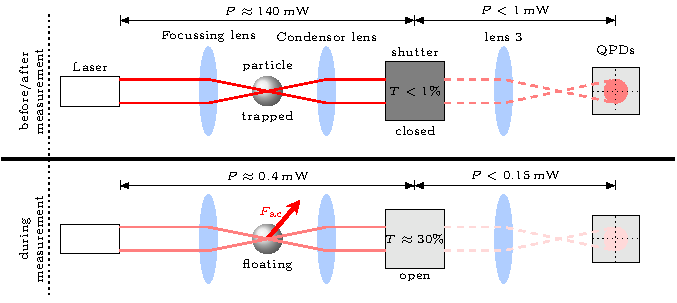
\includegraphics[width=\textwidth]{External/PU-protocol.pdf}
  \caption{Schematic of optical trapping setup, laser settings ($P$: laser 
    power), and optical shutter settings ($T$: transmittance for $\llaser = 
    \SI{785}{\nm}$) before and after the build up measurement (BM; top) and 
    during the BM (bottom). During the BM the particle is free floating, the 
    laser power is reduced as low as possible, the shutter is opened to allow 
    optical position detection on the quadrant photo detectors (QPDs), and the 
    ultrasound is switched on; hence there acts an acoustic force 
    $F_{\mathrm{ac}}$ on the particle. Before and after the BM all states are 
switched to their respective opposite.}\label{fig:PU-protocol}
\end{figure*}

Our OT consists of a single laser with a maximal power of \SI{200}{\milli\watt} 
and a wavelength of $\llaser = \SI{785}{\nm}$ (Omicron GmbH, Rodgau, Germany). 
The laser traps a spherical \SiO~particle with a radius of $R=\SI{1.03}{\um}$ 
(Microparticle GmbH, Berlin, Germany; same as in \cite{Goering2021}) and acts 
also as the light source for the displacement signal on the QPDs (see 
\cref{fig:PU-protocol}). The \SiO~particles have the advantage that they are 
hydrophilic which makes handling with our OT easier. As shown 
in~\cite{Goering2021} the critical radius for our experimental settings is 
$\Rcrit\approx\SI{0.6}{\um}$ which makes the movement of the used particles ARF 
dominated. Nevertheless, we can separate the AS and ARF induced movement 
because the effects are for our BM locations orthogonal to each other.

In the normal trapping mode it is not possible to measure the build up of AS 
and the ARF because the timeconstant of the OT ($\tau_{\mathrm{OT}}\approx 
\SI{1.59}{\ms}$ \cite{Goering2021}) is much larger than the ones of interest 
($\tau_{\mathrm{AS}}\approx \SI{1.44}{\ms}$ and $\tau_{\mathrm{ARF}}\approx 
\SI{1.4}{\us}$ \cite{Goering2021}). $\tau_{\mathrm{ARF}}$ is defined as the 
build up time of the ARF, which is approximated by the build up time $\tau$ of 
a single degree of freedom acoustic resonance mode with quality factor 
$Q\approx 40$ and $\tau_{\mathrm{AS}}$ is the momentum diffusion 
time~\cite{Muller2015}. Therefore, we need to switch the laser almost 
completely off such that the formerly stably trapped particle becomes 
free-floating. If the particle is free-floating, there is no influence from the 
OT characteristics on the BM.

For stable trapping of our particles the laser power must be greater than at 
least \SI{75}{\milli\watt}. However, this laser intensity is too high for the 
QPDs in the back focal plane and they would be damaged without further 
modifications. Therefore, an optical shutter (FOS NIR 1100, LC-TEC, Borlänge, 
Sweden) is installed in the laser path before the QPDs (see 
\cref{fig:PU-protocol}). The shutter transmittance $T$ is proportional to the 
applied voltage of the shutter driving signal. In earlier experiments with our 
OT the optical shutter was implemented as a fixed set of neutral density 
filters that limited the transmitted intensity to less than 0.1\% of the 
trapping intensity \cite{Lakaemper2015,Lamprecht2016,Lamprecht2021}. Before and 
after our BMs the particle is stably trapped.

One single BM follows the sketched process of \cref{fig:PU-flowchart} (see also 
\cref{fig:PU-protocol}). The particle is free floating during the BM and 
re-trapped at the end. The spot size of the OT is not finite and re-trapping to 
the exact same location unlikely. Therefore at the beginning of each BM the 
Python control software checks if the offset of the QPDs needs to be adjusted. 
A QPD with zero offset is in the middle of the linear regime between the 
displacement of the particle and the measured voltage at the QPDs. Hence, the 
offset adjustment before a new BM enables the quantitative comparison between 
BMs because all begin with the same offset. If an adjustment is necessary, an 
automated incremental offset change is performed and the QPD values are checked 
again. If there is no action needed, the laser changes its power $P$ from 
\SI{140}{\milli\watt} to \SI{0.4}{\milli\watt} and the shutter starts to open. 
The laser power change takes effect in less than \SI{3}{\ms}, whereas the 
shutter is specified to open within \SI{15}{\ms} from fully closed to 90\% of 
its fully open state. To ensure the shutter is maximally opened we wait another 
\SI{10}{\ms} before the ultrasound (US) is switched on. In this first 
\SI{25}{\ms} ($t=\SI{-25}{\ms}$ to $t=\SI{0}{\ms}$) the particle is free 
floating and will therefore start sedimenting. We showed in \cite{Goering2021} 
that the particle travels less than $\SI{0.052}{\um}\approx 0.05\,R$ in this 
time towards the bottom of the device. This distance is uncritical for the 
further BM. At $t=\SI{0}{\ms}$ the US is switched on for \SI{30}{\ms}. The 
particle is displaced due to the acoustic forces $F_{\mathrm{ac}}$. At 
$t=\SI{55}{\ms}$, the shutter starts closing and the laser power is increased 
to its starting power again to retrap the same free-floating particle. After 
the output of the data a new BM starts. The time between two consecutive BMs 
is more than \SI{2}{\s}. The data for one BM is collected over a timespan of 
\SI{100}{\ms} where the US is switched on for \SI{30}{\ms} only. The acoustic 
excitation frequency $\fex$ is set to the same value of \SI{4.015}{\mega\hertz} 
where we measured 17 standing pressure nodal planes. With a maximal force 
amplitude of \SI{1.25}{\pico\newton} for a \SI{4.39}{\um} diameter particle and 
a maximal force amplitude of \SI{0.17}{\pico\newton} for a \SI{2.06}{\um} 
diameter particle (both measured with the OT~\cite{Goering2021}) and the 
assumption of an one dimensional pressure wave the acoustic pressure (see 
equations (30a) through (30c) in~\cite{Bruus2012}) inside the fluid cavity is 
about \SI{100}{\kilo\pascal}~\cite{Goering2021}. With this short time of US 
excitation and the fast build up constant for the ARF 
($\tau_{\mathrm{ARF}}\approx \SI{1.4}{\us}$) compared to the relatively long 
time between BMs, the system has the same starting conditions for each BM 
respectively.

\begin{figure*}[tbp]
  \centering
  % \tikzsetnextfilename{flowchart}
{
  \footnotesize

\begin{tikzpicture}[node distance=1cm]

  \node (start) [startstop] {Start\\[-3.5mm] measurement};
  \node (qpd) [io, right of=start, xshift=30mm, yshift=15mm] {Need 
  QPD\\[-3.5mm] adjustment?};
\node (pqpd) [process, left of=qpd, xshift=-30mm] {Adjust QPD};
\node (mea1) [mea, right of=qpd, xshift=30mm] {Reduce $P$\\[-3.5mm] Open 
shutter};
\node [time,right of=mea1, xshift=6mm, anchor=west] {$t=\SI{-25}{\ms}$};
\node (US) [io, below of=mea1, yshift=-8mm] {Ultrasound\\[-3.5mm]on?};
\node [time,right of=US, xshift=8mm, anchor=west] {$t=\SI{0}{\ms}$};
\node (mea2) [mea, below of=US, yshift=-8mm, xshift=20mm] {Start US};
\node (mea3) [mea, below of=US, yshift=-8mm, xshift=-20mm] {Close 
shutter\\[-3.5mm] Increase $P$};
\node [time, below of=mea3, yshift=4.5mm, anchor=north] {$t=\SI{55}{\ms}$};
\node (out) [process, left of=mea3, xshift=-30mm] {Store\\[-3.5mm] data};

\draw [arrow] (start) -| (qpd);
\draw [arrow] (qpd) -- node[anchor=south, above] {yes} (pqpd);
\draw [arrow] (pqpd) -- (start);
\draw [arrow] (qpd) -- node[anchor=south, above] {no} (mea1);
\draw [arrow] (mea1) -- (US);
\draw [arrow] (US) -- node[anchor=west, right] {yes} (mea2);
\draw [arrow] (US) -- node[anchor=east, left] {no} (mea3);
\draw [arrow] (mea2) -- (mea3);
\draw [arrow] (mea3) -- (out);
\draw [arrow] (out) -- (start);


\node (tr) at ($(mea1.north east)+(2.5,0.3)$) {};
\node (br) at ($(mea2.south east)+(0.5,-0.8)$) {};
\node [left of=br, yshift=3mm, text width=30mm] (text) {\textit{particle 
floating}};

\node (tl) at ($(mea1.north west)+(-0.1,0.3)$) {};
\node (ml) at ($(mea3.north west)+(-0.3,0.5)$) {};
\node (bl) at ($(mea3.south west)+(-0.3,-0.8)$) {};

\begin{scope}[on background layer]
  \draw[orange, thick, dotted, fill=orange!5] (bl.center) -- (ml.center) -- 
  (tl.center) -- (tr.center) -- (br.center) -- (bl.center);
\end{scope}


\end{tikzpicture}
}

  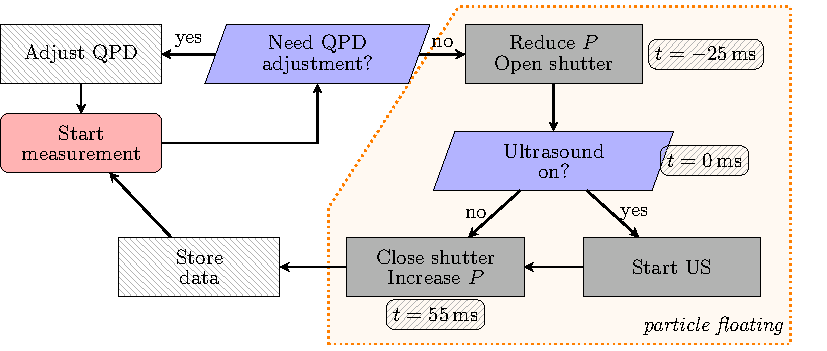
\includegraphics[width=\textwidth]{External/PU-flowchart.pdf}
  \caption{Process diagram for one measurement cycle. The gray rectangles 
    represent the processes during the build up measurement (BM). During this 
    time the particle is free floating (orange area). All process steps others 
    are before or after a BM. The timestamps in the hatched rounded 
    rectangles represent the times when the process attached to them is 
    executed. One measurement cycle takes about \SI{2}{\s} to be executed. The 
  BM itself is less than \SI{100}{\ms}.}\label{fig:PU-flowchart}
\end{figure*}

One whole measurement series consists of 6 different $\Dy_{i}$ positions, one 
fixed pulse frequency $\fp$, and one fixed duty percentage. Per $\Dy_{i}$ we 
perform 75 BMs with acoustic excitation (\emph{on BMs}) and 75 BMs without 
excitation (\emph{off BMs}). As result for this combination of pulse frequency 
$\fp$, position $\Dy_{i}$, and duty percentage we take the difference of the 
averaged \emph{on BMs} subtracted from the averaged \emph{off BMs} ($\DV_{i}= 
{\mathrm{avg.~\emph{on}}} - {\mathrm{avg.~\emph{off}}}$). While the BM is 
prepared, the first \SI{25}{\ms} are exactly the same between \emph{on} and 
\emph{off} BMs. The repetition per location $\Dy_{i}$ is necessary to reduce 
the unwanted noise from the Brownian motion. As in \cite{Goering2021}, we 
measure with a sampling frequency of \SI{1.25}{\mega\hertz} and average the 
measured data over a centered window of \SI{80}{\us} (101 data points).

Our BMs locations within the standing pressure field are the same as in 
\cite{Goering2021}. At those locations the forces from AS and the ARF itself 
were large enough in our device. All BMs are in the middle plane between the 
top and bottom fluid-device interface of our fluid cavity ($\Dz = 
\SI{0}{\um}$). Undisturbed Rayleigh streaming would lead to no streaming 
velocity in the middle plane along $\ez$. However, the excitation in our device 
is from one side only which leads to asymmetries in the AS field. These 
asymmetries result from the inclusion of the Stokes drift term in the numerical 
model as opposed to using a simplified limiting velocity approach for the AS 
calculation which does not include Stokes drift and lead to symmetrical 
streaming patterns while having an one-sided acoustic 
excitation~\cite{Hahn2016}. We have shown in~\cite{Goering2021} with a 
two-dimensional numerical simulations where we model the device-cavity 
cross-section as it is in the device that for our BM locations the streaming 
rolls can be over the whole channel height. Therefore, we can measure at $\Dz 
= \SI{0}{\um}$ a streaming velocity in $\ez$ direction.

All BMs for a certain pulse frequency $\fp=\sfrac{\fex}{k}$ were performed 
consecutively starting with a duty percentage of 100\% and going down to 50\% 
(see \cref{fig:PU-duty_cycle}). Between the different pulse frequencies $\fp$ the 
device was taken out of the OT setup, emptied, cleaned, and refilled. This 
procedure was necessary to ensure the same experimental conditions at the start 
and during the BMs because our device is a simple cavity with a 
\qtyproduct[product-units = bracket-power]{3 x 0.1}{\mm} cross-section etched 
in silicon with two open sides of the cavity (see \cref{fig:PU-device}). This 
rather wide channel dimension is necessary because of the large half cone angle 
of the laser beam ($\approx \SI{72}{\degree}$). The channel walls are 
non-transparent for the laser wavelength and hence a minimal distance must be 
kept from the channel walls to facilitate unhindered measurements.

To prevent evaporation of water during the experiments we seal both sides with 
a drop of silicone oil that is less likely to evaporate due to its higher 
viscosity. Nevertheless, at the end of one measurement series some water had 
left the channel. This change of water volume in the cavity is less than 5\% of 
its overall volume. The evaporation occurs at the sides of the cavity and does 
not lead to air bubbles within the cavity.

The disadvantage from this procedure is the dis- and reconnecting of the 
electric cables to the PZT, as well as the application of a new immersion layer 
on top of the device for the oil immersion lens of our OT. We limited the 
difference in immersion layer volume and initial placement, as well as cable 
connection between two different pulse frequencies $\fp$ to a minimum to ensure 
comparability between two different data sets. Nevertheless, there were small 
changes and we adapted the voltage at the function generator between the 
different pulse frequencies to have the same acoustic pressure $p_{\mathrm{a}}$ 
in the cavity and hence the same magnitude of the ARF and AS. We did this by 
comparing and adjusting the time it takes until the particle displacement is 
outside of the linear regime of the QPDs. This is a manual process and, hence, 
there are small differences in the experiments between different BM series.

% We adjusted the applied voltage such that the end of our measurement timeframe 
% coincides with the start of the non-linearity of the QPDs.

\begin{figure}[tbp]
  \centering
  % \tikzsetnextfilename{PU-duty-cycle}
{
  \small
%%%%%%%
% READ TABLE
%%%%%%%
\pgfplotstableread{\relPath/10_Figures/TikZ/duty_cycle.dat}{\data}

\begin{tikzpicture}[]
\begin{axis}[%
  x tick label style={
    /pgf/number format/.cd,
    fixed,
    fixed zerofill,
    precision=1
  },
  height=40mm,%
  width=84mm,%
  scale only axis,
   xlabel={Pulse cylces ($t\cdot \fp$ [-])},
   ylabel style={align=center},
   ylabel={},
   yticklabels={,,},
    legend style={
      fill=white!80!black,
      font=\tiny,
      at={(0.03,0.03)},
      anchor=south west
    },
   legend cell align={left},
   title={Pulsed Excitation Signal},]



      \addlegendimage{empty legend};

      \addplot[p100] table[x=time, y=duty_100] {\data};
      \addplot[p70] table[x=time, y=duty_70] {\data};
      \addplot[p50] table[x=time, y=duty_50] {\data};

      \addlegendentry{\hspace{-.6cm}Duty Cycle \%}
      \addlegendentry{100};
      \addlegendentry{70};
      \addlegendentry{50};

\end{axis}
\end{tikzpicture}
}

  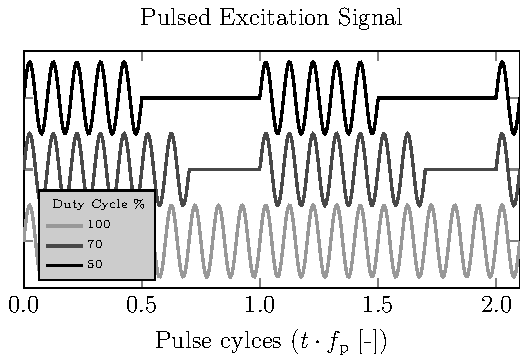
\includegraphics[]{External/PU-duty-cycle.pdf}
  \caption{Schematic of pulsed acoustic excitation for three different duty 
      percentages (50, 70, and 100\%) over pulsing cycles $t\cdot \fp$ with the 
      relation $\fex=k\,\fp$ (here $k=10$).
      %\textbf{15 words}
  }\label{fig:PU-duty_cycle}
\end{figure}

The pulse frequencies $\fp$ we chose such that the fraction $\sfrac{\fex}{\fp}$ 
is an integer $k$. This means that per pulsing cycle 
($T_{\mathrm{p}}=\sfrac{1}{\fp}$) $k$ excitation periods 
$t_{0}=\sfrac{1}{\fex}$ are within $1\,T_{\mathrm{p}}$. As integer we set 
$k\in\{1'000, 5'000, 10'000\}$. The investigated duty percentages are 100\%, 
90\%, 80\%, 70\%, 60\%, and 50\%. The percentage value reflects the relative 
time the excitation is switched on within $1\,T_{\mathrm{p}}$ (see 
\cref{fig:PU-duty_cycle}). The BM with 100\% duty (\emph{always on}) is the 
baseline where the excitation is on for the entire BM. This BM is used for 
normalizing all other duty percentages at the same point $\Dy_{i}$ and pulse 
frequency $\fp$. The shortest pulse duration is for $k=1000$ and 50\% duty 
width. With these settings 500 \emph{on}-periods are followed by 500 
\emph{off}-periods before starting all over. The pressure amplitude build up is 
proportional to $\propto\left[ 1-\exp\left( \sfrac{-t}{\tau_{\mathrm{ARF}}} 
\right) \right]$ for this linear oscillating system. After 
$\sfrac{50}{\fex}\approx\SI{12.5}{\us}$ (50 excitation periods) the system is 
at 99.96\% of its steady-state amplitude. Although our system is subjected to 
two frequencies ($\fex$ and $\fp$) there are no influences on the pressure wave 
frequency because the build up is much faster than the shortest pulse.

All in all, compared to \cite{Goering2021} these three changes in the 
experimental settings are present: 1) 75 instead of 50 repetitions, 2) fixed 
$\Dz$ to \SI{0}{\um}, and 3) pulsed excitation signal.

%%%%%%%%%%%%%%%%%%%%%%%%%%%%%%%%%%%%%%%%%%%%%%%%%%%%%%%%%%%%%%%%%%%%%%%%%%%%%%
%%%%%%%%%%%%%%%%%%%%%%%%%%%%%%%%%%%%%%%%%%%%%%%%%%%%%%%%%%%%%%%%%%%%%%%%%%%%%%
\section{Results and Discussion}

Before discussing our results, we want to emphasize that our experiments are 
very sensitive to external disturbances as well as the experimental condition. 
Because the whole experiment was newly initialised between the different $k$ 
values and, therefore, experimental conditions might change slightly, the 
results of different $k$ values are not fully quantitatively comparable. 
However, the trend for different $k$ values are nevertheless conclusive.

\begin{figure*}[tbp]
  \centering
  % \tikzsetnextfilename{PU-duty-m04}
{
  \small
%%%%%%%
% READ TABLE
%%%%%%%
\pgfplotstableread{\relPath/10_Figures/TikZ/duty_fp_1000.dat}{\dataOne}
\pgfplotstableread{\relPath/10_Figures/TikZ/duty_fp_5000.dat}{\dataTwo}
\pgfplotstableread{\relPath/10_Figures/TikZ/duty_fp_10000.dat}{\dataThree}
%%%%%%%
% LINES FOR ALL GROUPPLOTS
%%%%%%%
\renewcommand{\tikzHelper}{
  \fill[fill=black!10!white] (axis cs:-80,0) rectangle (axis cs:0,1);

  \draw[dotted] (axis cs:0,0) -- (axis cs:0,1);
  \draw[dotted] (axis cs:50,0) -- (axis cs:50,1);
  \draw[dotted] (axis cs:100,0) -- (axis cs:100,1);
  \draw[dotted] (axis cs:-80,0.5) -- (axis cs:120,0.5);
  \draw[dotted] (axis cs:-80,0.5) -- (axis cs:120,0.5);
}

\renewcommand{\tmp}{04}

\begin{tikzpicture}
   \begin{groupplot}[%
       scale only axis,
       axis on top,
       group style={
         group size= 2 by 3,
         group name=plots,
         vertical sep=6pt,%
         horizontal sep=8pt},%
       height=40mm,%
       width=64mm,%
        xticklabel style={
          /pgf/number format/fixed,
          /pgf/number format/precision=2
        }]

%%%%%%
%%% PLOT (1,1)
%%%%%%

   \nextgroupplot[%
     legend cell align={left},
     legend style={
        fill=black!10!white,
        font=\tiny,
        at={(0.02,0.95)},
        anchor=north west,
        /tikz/column 2/.style={column sep=1pt,},
        legend columns=2,
      },
     xticklabels={,,},
     % title={$\DV_{y}\,|\,\Dy = \SI{-0.06}{\milli\meter}$},%
     % title={Data for $y$-component},%
     title={ARF},%
     ylabel={$\sfrac{\DV_{j}}{\DV_{100,\text{max}}}$ },
 ]

      \tikzHelper

      \addlegendimage{empty legend}
      \addlegendimage{empty legend}

      \addplot[style100] table[x=dt, y=DV_y_m\tmp_100_m00] {\dataOne};
      \addplot[style90] table[x=dt, y=DV_y_m\tmp_090_m00] {\dataOne};
      \addplot[style80] table[x=dt, y=DV_y_m\tmp_080_m00] {\dataOne};
      \addplot[style70] table[x=dt, y=DV_y_m\tmp_070_m00] {\dataOne};
      \addplot[style60] table[x=dt, y=DV_y_m\tmp_060_m00] {\dataOne};
      \addplot[style50] table[x=dt, y=DV_y_m\tmp_050_m00] {\dataOne};


      \addlegendentry{\hspace{-6mm}\textbf{Duty \%}}
      \addlegendentry{\textbf{\phantom{a}}}
      \addlegendentry{100};
      \addlegendentry{90};
      \addlegendentry{80};
      \addlegendentry{70};
      \addlegendentry{60};
      \addlegendentry{50};


%%%%%%
%%% PLOT (1,2)
%%%%%%

   \nextgroupplot[%
     xticklabels={,,},
     yticklabels={,,},
     % title={Data for $z$-component}]%
     title={AS}]%

      \tikzHelper
      \draw[thick,|<->|] (axis cs:-80,0.25) -- (axis cs:0,0.25) node[midway, 
      above] {US off};

      \addplot[style100] table[x=dt, y=DV_z_m\tmp_100_m00] {\dataOne};
      \addplot[style90] table[x=dt, y=DV_z_m\tmp_090_m00] {\dataOne};
      \addplot[style80] table[x=dt, y=DV_z_m\tmp_080_m00] {\dataOne};
      \addplot[style70] table[x=dt, y=DV_z_m\tmp_070_m00] {\dataOne};
      \addplot[style60] table[x=dt, y=DV_z_m\tmp_060_m00] {\dataOne};
      \addplot[style50] table[x=dt, y=DV_z_m\tmp_050_m00] {\dataOne};

%%%%%%
%%% PLOT (2,1)
%%%%%%

   \nextgroupplot[%
     xticklabels={,,},
     ylabel={$\sfrac{\DV_{j}}{\DV_{100,\text{max}}}$ },
   ]

      \tikzHelper

      \addplot[style100] table[x=dt, y=DV_y_m\tmp_100_m00] {\dataTwo};
      \addplot[style90] table[x=dt, y=DV_y_m\tmp_090_m00] {\dataTwo};
      \addplot[style80] table[x=dt, y=DV_y_m\tmp_080_m00] {\dataTwo};

%%%%%%
%%% PLOT (2,2)
%%%%%%

   \nextgroupplot[%
     xticklabels={,,},
     yticklabels={,,},
   ]

      \tikzHelper

      \addplot[style100] table[x=dt, y=DV_z_m\tmp_100_m00] {\dataTwo};
      \addplot[style90] table[x=dt, y=DV_z_m\tmp_090_m00] {\dataTwo};
      \addplot[style80] table[x=dt, y=DV_z_m\tmp_080_m00] {\dataTwo};

%%%%%%
%%% PLOT (3,1)
%%%%%%

   \nextgroupplot[%
     ylabel={$\sfrac{\DV_{j}}{\DV_{100,\text{max}}}$ },
     xlabel={$10^{3}\,\sfrac{t}{t_{0}}$ [-]},
   ]

      \tikzHelper

      \addplot[style100] table[x=dt, y=DV_y_m\tmp_100_m00] {\dataThree};
      \addplot[style90] table[x=dt, y=DV_y_m\tmp_090_m00] {\dataThree};
      \addplot[style80] table[x=dt, y=DV_y_m\tmp_080_m00] {\dataThree};
      \addplot[style70] table[x=dt, y=DV_y_m\tmp_070_m00] {\dataThree};
      \addplot[style60] table[x=dt, y=DV_y_m\tmp_060_m00] {\dataThree};
      \addplot[style50] table[x=dt, y=DV_y_m\tmp_050_m00] {\dataThree};

      \foreach \val/\index in
      {50/0.120,60/0.143,70/0.178,80/0.232,90/0.281,100/0.312,110/0.367,120/0.44} {
        \edef\temp{\noexpand
        \draw[] (axis cs:\val, 0) -- (axis cs:\val,\index);
        }
        \temp}


%%%%%%
%%% PLOT (3,2)
%%%%%%

   \nextgroupplot[%
     yticklabels={,,},
     xlabel={$10^{3}\,\sfrac{t}{t_{0}}$ [-]},
     % title={$\Dy = \SI{-0.04}{\milli\meter}$}
   ]

      \tikzHelper

      \addplot[style100] table[x=dt, y=DV_z_m\tmp_100_m00] {\dataThree};
      \addplot[style90] table[x=dt, y=DV_z_m\tmp_090_m00] {\dataThree};
      \addplot[style80] table[x=dt, y=DV_z_m\tmp_080_m00] {\dataThree};
      \addplot[style70] table[x=dt, y=DV_z_m\tmp_070_m00] {\dataThree};
      \addplot[style60] table[x=dt, y=DV_z_m\tmp_060_m00] {\dataThree};
      \addplot[style50] table[x=dt, y=DV_z_m\tmp_050_m00] {\dataThree};


  \end{groupplot}

%%%%%%
%%% TEXT NEXT TO PLOTS
%%%%%%
  \node[above] at ($(plots c1r1.north west)!0.5!(plots c2r1.north east)$) 
  [yshift=10mm] {$\Dy = \SI{-0.\tmp}{\mm}$};

  \node[below] at ($(plots c1r3.south west)!0.5!(plots c2r3.south east)$) 
  [yshift=-10mm] {Excitation period};

  \node[rotate=90] at (plots c2r2.east) [yshift=-5mm] {$k$};
  \node[rotate=90] at (plots c2r1.east) [yshift=-10mm] {1000};
  \node[rotate=90] at (plots c2r2.east) [yshift=-10mm] {5000};
  \node[rotate=90] at (plots c2r3.east) [yshift=-10mm] {10000};

\end{tikzpicture}
}

  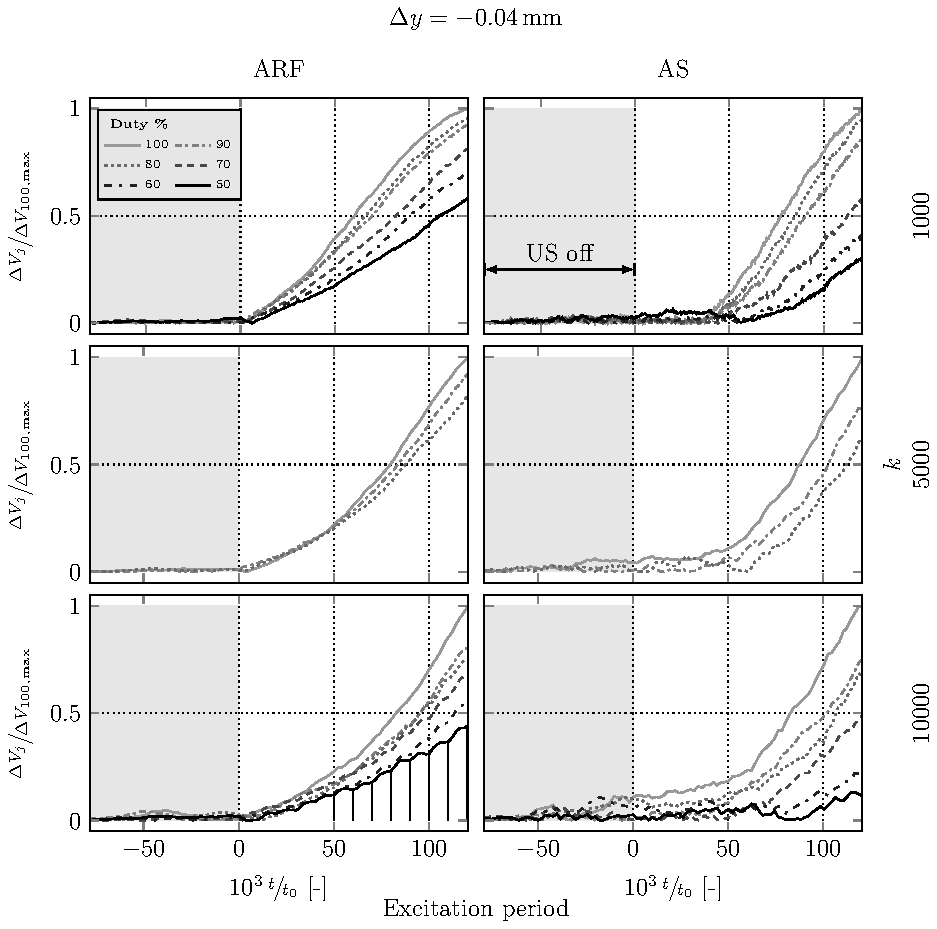
\includegraphics[]{External/PU-duty-m04.pdf}
  \caption{Evolution of averaged voltage differences $\DV_{y}$ (left column; 
    ARF associated) and $\DV_{z}$ (right column; AS associated) for three 
    different pulsing frequencies $\fp$ and different duty percentages at 
    $\Dy=\SI{-0.4}{\mm}$ over excitation periods $\sfrac{t}{t_{0}}$ with 
    $t_{0}=\sfrac{1}{\fex}$. For the first row $\fp=\sfrac{\fex}{1'000}$, for 
    the second $\fp=\sfrac{\fex}{5'000}$, and for the last row 
    $\fp=\sfrac{\fex}{10'000}$. The data per plot is normalized to the maximal 
    amplitude of the data series with a duty percentage of 100\%. The gray 
    shaded area of each plot marks the time when the US is off. Additionally, 
    the vertical solid lines in the bottom left plot mark the beginning of a 
    new pulsing cycle.
    %\textbf{80 words}
}\label{fig:PU-duty-m04}
\end{figure*}

\begin{figure*}[tbp]
  \centering
  % \tikzsetnextfilename{PU-duty-m05}
{
  \small
%%%%%%%
%%%%%%%
% READ TABLE
%%%%%%%
\pgfplotstableread{\relPath/10_Figures/TikZ/duty_fp_1000.dat}{\dataOne}
\pgfplotstableread{\relPath/10_Figures/TikZ/duty_fp_5000.dat}{\dataTwo}
\pgfplotstableread{\relPath/10_Figures/TikZ/duty_fp_10000.dat}{\dataThree}
%%%%%%%
% LINES FOR ALL GROUPPLOTS
%%%%%%%
\renewcommand{\tikzHelper}{
  \fill[fill=black!10!white] (axis cs:-80,0) rectangle (axis cs:0,1);

  \draw[dotted] (axis cs:0,0) -- (axis cs:0,1);
  \draw[dotted] (axis cs:50,0) -- (axis cs:50,1);
  \draw[dotted] (axis cs:100,0) -- (axis cs:100,1);
  \draw[dotted] (axis cs:-80,0.5) -- (axis cs:120,0.5);
  \draw[dotted] (axis cs:-80,0.5) -- (axis cs:120,0.5);
}


\begin{tikzpicture}
   \begin{groupplot}[%
       scale only axis,
       axis on top,
       group style={
         group size= 2 by 3,
         group name=plots,
         vertical sep=6pt,%
         horizontal sep=8pt},%
       height=40mm,%
       width=64mm,%
        xticklabel style={
          /pgf/number format/fixed,
          /pgf/number format/precision=2
        }]

%%%%%%
%%% PLOT (1,1)
%%%%%%

   \nextgroupplot[%
     legend cell align={left},
     legend style={
        fill=black!10!white,
        font=\tiny,
        at={(0.02,0.95)},
        anchor=north west,
        /tikz/column 2/.style={column sep=1pt,},
        legend columns=2,
      },
     xticklabels={,,},
     % title={$\DV_{y}\,|\,\Dy = \SI{-0.06}{\milli\meter}$},%
     title={ARF},%
     % title={Data for $y$-component},%
     ylabel={$\sfrac{\DV_{j}}{\DV_{100,\text{max}}}$ },
 ]

      \tikzHelper

      \addlegendimage{empty legend}
      \addlegendimage{empty legend}

      \addplot[style100] table[x=dt, y=DV_y_m05_100_m00] {\dataOne};
      \addplot[style90] table[x=dt, y=DV_y_m05_090_m00] {\dataOne};
      \addplot[style80] table[x=dt, y=DV_y_m05_080_m00] {\dataOne};
      \addplot[style70] table[x=dt, y=DV_y_m05_070_m00] {\dataOne};
      \addplot[style60] table[x=dt, y=DV_y_m05_060_m00] {\dataOne};
      \addplot[style50] table[x=dt, y=DV_y_m05_050_m00] {\dataOne};


      \addlegendentry{\hspace{-6mm}\textbf{Duty \%}}
      \addlegendentry{\textbf{\phantom{a}}}
      \addlegendentry{100};
      \addlegendentry{90};
      \addlegendentry{80};
      \addlegendentry{70};
      \addlegendentry{60};
      \addlegendentry{50};


%%%%%%
%%% PLOT (1,2)
%%%%%%

   \nextgroupplot[%
     xticklabels={,,},
     yticklabels={,,},
     % title={Data for $z$-component}]%
     title={AS},
   ]%

      \tikzHelper
      \draw[thick,|<->|] (axis cs:-80,0.25) -- (axis cs:0,0.25) node[midway, 
      above] {US off};

      \addplot[style100] table[x=dt, y=DV_z_m05_100_m00] {\dataOne};
      \addplot[style90] table[x=dt, y=DV_z_m05_090_m00] {\dataOne};
      \addplot[style80] table[x=dt, y=DV_z_m05_080_m00] {\dataOne};
      \addplot[style70] table[x=dt, y=DV_z_m05_070_m00] {\dataOne};
      \addplot[style60] table[x=dt, y=DV_z_m05_060_m00] {\dataOne};
      \addplot[style50] table[x=dt, y=DV_z_m05_050_m00] {\dataOne};

%%%%%%
%%% PLOT (2,1)
%%%%%%

   \nextgroupplot[%
     xticklabels={,,},
     ylabel={$\sfrac{\DV_{j}}{\DV_{100,\text{max}}}$ },
   ]

      \tikzHelper

      \addplot[style100] table[x=dt, y=DV_y_m05_100_m00] {\dataTwo};
      \addplot[style90] table[x=dt, y=DV_y_m05_090_m00] {\dataTwo};
      \addplot[style80] table[x=dt, y=DV_y_m05_080_m00] {\dataTwo};

%%%%%%
%%% PLOT (2,2)
%%%%%%

   \nextgroupplot[%
     xticklabels={,,},
     yticklabels={,,},
   ]

      \tikzHelper

      \addplot[style100] table[x=dt, y=DV_z_m05_100_m00] {\dataTwo};
      \addplot[style90] table[x=dt, y=DV_z_m05_090_m00] {\dataTwo};
      \addplot[style80] table[x=dt, y=DV_z_m05_080_m00] {\dataTwo};

%%%%%%
%%% PLOT (3,1)
%%%%%%

   \nextgroupplot[%
     ylabel={$\sfrac{\DV_{j}}{\DV_{100,\text{max}}}$ },
     xlabel={$10^{3}\,\sfrac{t}{t_{0}}$ },
   ]

      \tikzHelper

      \addplot[style100] table[x=dt, y=DV_y_m05_100_m00] {\dataThree};
      \addplot[style90] table[x=dt, y=DV_y_m05_090_m00] {\dataThree};
      \addplot[style80] table[x=dt, y=DV_y_m05_080_m00] {\dataThree};
      \addplot[style70] table[x=dt, y=DV_y_m05_070_m00] {\dataThree};
      \addplot[style60] table[x=dt, y=DV_y_m05_060_m00] {\dataThree};
      \addplot[style50] table[x=dt, y=DV_y_m05_050_m00] {\dataThree};

      \foreach \val/\index in 
      {50/0.104,60/0.138,70/0.161,80/0.205,90/0.241,100/0.277,110/0.310,120/0.36} {
        \edef\temp{\noexpand
        \draw[] (axis cs:\val, 0) -- (axis cs:\val,\index);
        }
        \temp}

%%%%%%
%%% PLOT (3,2)
%%%%%%

   \nextgroupplot[%
     yticklabels={,,},
     xlabel={$10^{3}\,\sfrac{t}{t_{0}}$ },
     % title={$\Dy = \SI{-0.04}{\milli\meter}$}
   ]

      \tikzHelper

      \addplot[style100] table[x=dt, y=DV_z_m05_100_m00] {\dataThree};
      \addplot[style90] table[x=dt, y=DV_z_m05_090_m00] {\dataThree};
      \addplot[style80] table[x=dt, y=DV_z_m05_080_m00] {\dataThree};
      \addplot[style70] table[x=dt, y=DV_z_m05_070_m00] {\dataThree};
      \addplot[style60] table[x=dt, y=DV_z_m05_060_m00] {\dataThree};
      \addplot[style50] table[x=dt, y=DV_z_m05_050_m00] {\dataThree};


  \end{groupplot}

%%%%%%
%%% TEXT NEXT TO PLOTS
%%%%%%
  \node[above] at ($(plots c1r1.north west)!0.5!(plots c2r1.north east)$) 
  [yshift=10mm] {$\Dy = \SI{-0.05}{\mm}$};

  \node[rotate=90] at (plots c2r2.east) [yshift=-5mm] {$k$};
  \node[rotate=90] at (plots c2r1.east) [yshift=-10mm] {1000};
  \node[rotate=90] at (plots c2r2.east) [yshift=-10mm] {5000};
  \node[rotate=90] at (plots c2r3.east) [yshift=-10mm] {10000};

\end{tikzpicture}
}

  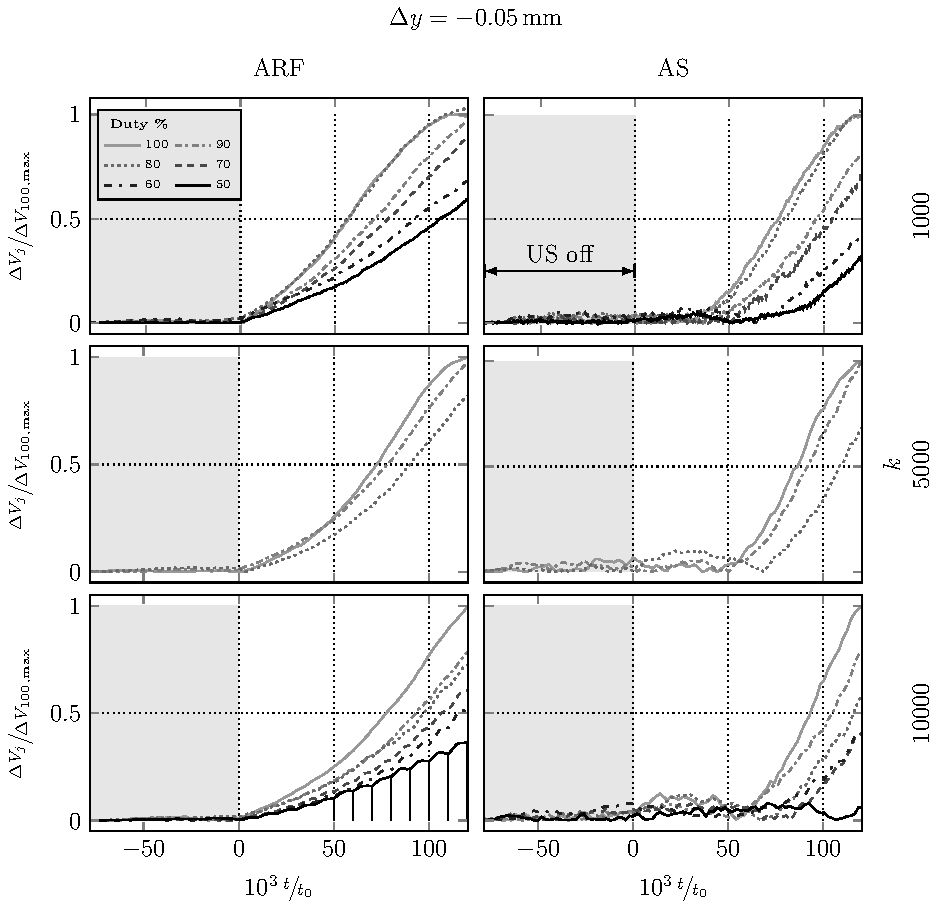
\includegraphics[]{External/PU-duty-m05.pdf}
  \caption{Evolution of averaged voltage differences $\DV_{y}$ (left column; 
    ARF associated) and $\DV_{z}$ (right column; AS associated) for three 
    different pulsing frequencies $\fp$ and different duty percentages at 
    $\Dy=\SI{-0.5}{\mm}$ over excitation periods $\sfrac{t}{t_{0}}$ with 
    $t_{0}=\sfrac{1}{\fex}$. For the first row $\fp=\sfrac{\fex}{1'000}$, for 
    the second $\fp=\sfrac{\fex}{5'000}$, and for the last row 
    $\fp=\sfrac{\fex}{10'000}$. The data per plot is normalized to the maximal 
    amplitude of the data series with a duty percentage of 100\%. The gray 
    shaded area of each plot marks the time when the US is off. Additionally, 
    the vertical solid lines in the bottom left plot mark the beginning of a 
    new pulsing cycle.
    %\textbf{80 words}
}\label{fig:PU-duty-m05}
\end{figure*}

\begin{figure*}[tbp]
  \centering
  % \tikzsetnextfilename{duty-m06}
{
  \small
%%%%%%%
% READ TABLE
%%%%%%%
\pgfplotstableread{SECTION/15_Figures/duty_fp_1000.dat}{\dataOne}
\pgfplotstableread{SECTION/15_Figures/duty_fp_5000.dat}{\dataTwo}
\pgfplotstableread{SECTION/15_Figures/duty_fp_10000.dat}{\dataThree}
%%%%%%%
% LINES FOR ALL GROUPPLOTS
%%%%%%%
\renewcommand{\tikzHelper}{
  \fill[fill=black!10!white] (axis cs:-80,0) rectangle (axis cs:0,1);

  \draw[dotted] (axis cs:0,0) -- (axis cs:0,1);
  \draw[dotted] (axis cs:50,0) -- (axis cs:50,1);
  \draw[dotted] (axis cs:100,0) -- (axis cs:100,1);
  \draw[dotted] (axis cs:-80,0.5) -- (axis cs:120,0.5);
  \draw[dotted] (axis cs:-80,0.5) -- (axis cs:120,0.5);
}

\renewcommand{\tmp}{06}

\begin{tikzpicture}
   \begin{groupplot}[%
       scale only axis,
       group style={
         group size= 2 by 3,
         group name=plots,
         vertical sep=4pt,%
         horizontal sep=8pt},%
       height=25mm,%
       width=64mm,%
        xticklabel style={
          /pgf/number format/fixed,
          /pgf/number format/precision=2
        }]

%%%%%%
%%% PLOT (1,1)
%%%%%%

   \nextgroupplot[%
     legend cell align={left},
     legend style={
        fill=black!10!white,
        font=\tiny,
        at={(0.02,0.95)},
        anchor=north west,
        /tikz/column 2/.style={column sep=1pt,},
        legend columns=2,
      },
     xticklabels={,,},
     % title={Data for $y$-component},%
     title={ARF},%
     ylabel={$\sfrac{\DV_{j}}{\DV_{100,\text{max}}}$ },
 ]

      \tikzHelper

      \addlegendimage{empty legend}
      \addlegendimage{empty legend}

      \addplot[style100] table[x=dt, y=DV_y_m\tmp_100_m00] {\dataOne};
      \addplot[style90] table[x=dt, y=DV_y_m\tmp_090_m00] {\dataOne};
      \addplot[style80] table[x=dt, y=DV_y_m\tmp_080_m00] {\dataOne};
      \addplot[style70] table[x=dt, y=DV_y_m\tmp_070_m00] {\dataOne};
      \addplot[style60] table[x=dt, y=DV_y_m\tmp_060_m00] {\dataOne};
      \addplot[style50] table[x=dt, y=DV_y_m\tmp_050_m00] {\dataOne};


      \addlegendentry{\hspace{-6mm}\textbf{Duty \% }}
      \addlegendentry{\textbf{\phantom{a}}}
      \addlegendentry{100};
      \addlegendentry{90};
      \addlegendentry{80};
      \addlegendentry{70};
      \addlegendentry{60};
      \addlegendentry{50};


%%%%%%
%%% PLOT (1,2)
%%%%%%

   \nextgroupplot[%
     xticklabels={,,},
     yticklabels={,,},
     % title={Data for $z$-component},
     title={AS},
   ]%

      \tikzHelper
      \draw[thick,|<->|] (axis cs:-80,0.25) -- (axis cs:0,0.25) node[midway, 
      above] {US off};

      \addplot[style100] table[x=dt, y=DV_z_m\tmp_100_m00] {\dataOne};
      \addplot[style90] table[x=dt, y=DV_z_m\tmp_090_m00] {\dataOne};
      \addplot[style80] table[x=dt, y=DV_z_m\tmp_080_m00] {\dataOne};
      \addplot[style70] table[x=dt, y=DV_z_m\tmp_070_m00] {\dataOne};
      \addplot[style60] table[x=dt, y=DV_z_m\tmp_060_m00] {\dataOne};
      \addplot[style50] table[x=dt, y=DV_z_m\tmp_050_m00] {\dataOne};

%%%%%%
%%% PLOT (2,1)
%%%%%%

   \nextgroupplot[%
     xticklabels={,,},
     ylabel={$\sfrac{\DV_{j}}{\DV_{100,\text{max}}}$ },
   ]

      \tikzHelper

      \addplot[style100] table[x=dt, y=DV_y_m\tmp_100_m00] {\dataTwo};
      \addplot[style90] table[x=dt, y=DV_y_m\tmp_090_m00] {\dataTwo};
      \addplot[style80] table[x=dt, y=DV_y_m\tmp_080_m00] {\dataTwo};

%%%%%%
%%% PLOT (2,2)
%%%%%%

   \nextgroupplot[%
     xticklabels={,,},
     yticklabels={,,},
   ]

      \tikzHelper

      \addplot[style100] table[x=dt, y=DV_z_m\tmp_100_m00] {\dataTwo};
      \addplot[style90] table[x=dt, y=DV_z_m\tmp_090_m00] {\dataTwo};
      \addplot[style80] table[x=dt, y=DV_z_m\tmp_080_m00] {\dataTwo};

%%%%%%
%%% PLOT (3,1)
%%%%%%

   \nextgroupplot[%
     ylabel={$\sfrac{\DV_{j}}{\DV_{100,\text{max}}}$ },
     xlabel={$10^{3}\,\sfrac{t}{t_{0}}$ },
   ]

      \tikzHelper

      \addplot[style100] table[x=dt, y=DV_y_m\tmp_100_m00] {\dataThree};
      \addplot[style90] table[x=dt, y=DV_y_m\tmp_090_m00] {\dataThree};
      \addplot[style80] table[x=dt, y=DV_y_m\tmp_080_m00] {\dataThree};
      \addplot[style70] table[x=dt, y=DV_y_m\tmp_070_m00] {\dataThree};
      \addplot[style60] table[x=dt, y=DV_y_m\tmp_060_m00] {\dataThree};
      \addplot[style50] table[x=dt, y=DV_y_m\tmp_050_m00] {\dataThree};


      \foreach \val/\index in 
      {50/0.108,60/0.132,70/0.158,80/0.188,90/0.221,100/0.252,110/0.301,120/0.35} {
        \edef\temp{\noexpand
        \draw[] (axis cs:\val, 0) -- (axis cs:\val,\index);
        }
        \temp}
%%%%%%
%%% PLOT (3,2)
%%%%%%

   \nextgroupplot[%
     yticklabels={,,},
     xlabel={$10^{3}\,\sfrac{t}{t_{0}}$ },
   ]

      \tikzHelper

      \addplot[style100] table[x=dt, y=DV_z_m\tmp_100_m00] {\dataThree};
      \addplot[style90] table[x=dt, y=DV_z_m\tmp_090_m00] {\dataThree};
      \addplot[style80] table[x=dt, y=DV_z_m\tmp_080_m00] {\dataThree};
      \addplot[style70] table[x=dt, y=DV_z_m\tmp_070_m00] {\dataThree};
      \addplot[style60] table[x=dt, y=DV_z_m\tmp_060_m00] {\dataThree};
      \addplot[style50] table[x=dt, y=DV_z_m\tmp_050_m00] {\dataThree};


  \end{groupplot}

%%%%%%
%%% TEXT NEXT TO PLOTS
%%%%%%
  \node[above] at ($(plots c1r1.north west)!0.5!(plots c2r1.north east)$) 
  [yshift=10mm] {$\Dy = \SI{-0.\tmp}{\mm}$};

  \node[rotate=90] at (plots c2r2.east) [yshift=-5mm] 
  {$\fp=\sfrac{\fex}{\bullet}$};
  \node[rotate=90] at (plots c2r1.east) [yshift=-10mm] {1000};
  \node[rotate=90] at (plots c2r2.east) [yshift=-10mm] {5000};
  \node[rotate=90] at (plots c2r3.east) [yshift=-10mm] {10000};

\end{tikzpicture}
}

  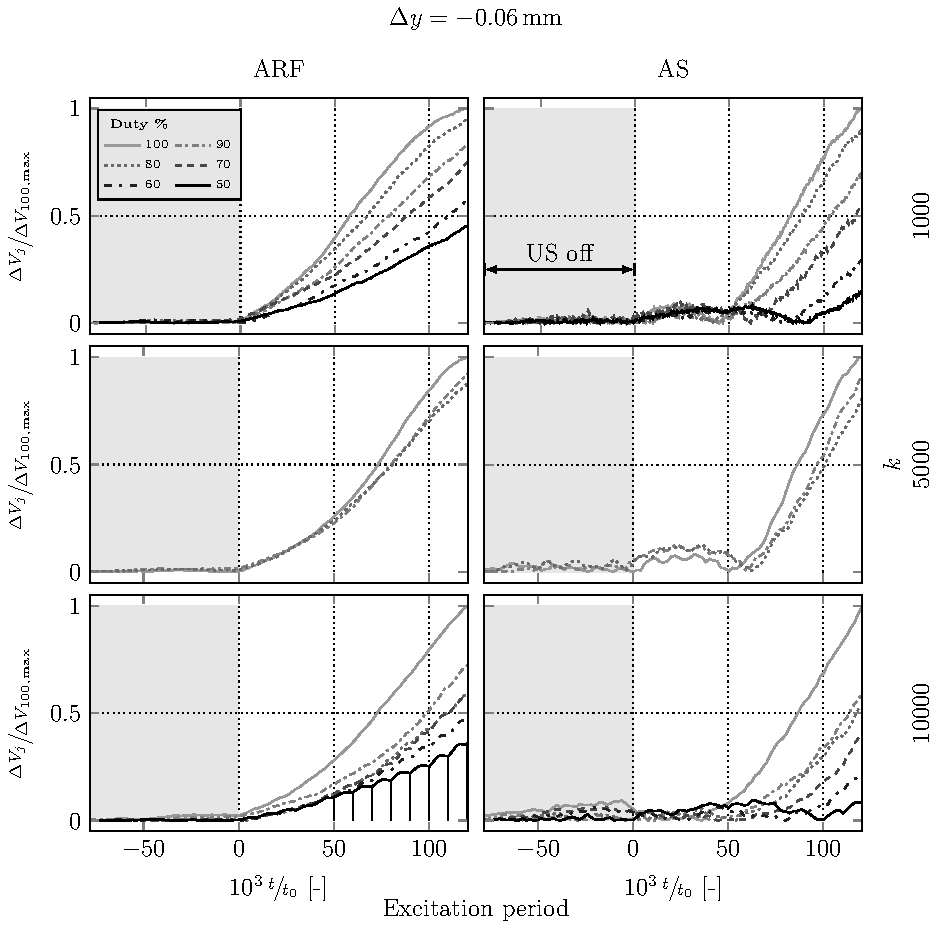
\includegraphics[]{External/PU-duty-m06.pdf}
  \caption{Evolution of averaged voltage differences $\DV_{y}$ (left column; 
    ARF associated) and $\DV_{z}$ (right column; AS associated) for three 
    different pulsing frequencies $\fp$ and different duty percentages at 
    $\Dy=\SI{-0.6}{\mm}$ over excitation periods $\sfrac{t}{t_{0}}$ with 
    $t_{0}=\sfrac{1}{\fex}$. For the first row $\fp=\sfrac{\fex}{1'000}$, for 
    the second $\fp=\sfrac{\fex}{5'000}$, and for the last row 
    $\fp=\sfrac{\fex}{10'000}$. The data per plot is normalized to the maximal 
    amplitude of the data series with a duty percentage of 100\%. The gray 
    shaded area of each plot marks the time when the US is off. Additionally, 
    the vertical solid lines in the bottom left plot mark the beginning of a 
    new pulsing cycle.
    %\textbf{80 words}
}\label{fig:PU-duty-m06}
\end{figure*}


In \cref{fig:PU-duty-m04,fig:PU-duty-m05,fig:PU-duty-m06} the results of the BMs over 
time for $\Dy_{i}=\SI{-0.04}{\mm}$, $\Dy_{i}=\SI{-0.05}{\mm}$, 
$\Dy_{i}=\SI{-0.06}{\mm}$ are plotted, respectively. The figures consist of two 
columns (left for the ARF build up and right for the AS build up) and three 
rows for the three different pulsing frequencies $\fp$; in the 
1\textsuperscript{st} row $\fp=\sfrac{\fex}{1'000}$, in the 
2\textsuperscript{nd} row $\fp=\sfrac{\fex}{5'000}$, and in the 
3\textsuperscript{rd} row $\fp=\sfrac{\fex}{10'000}$, respectively. For 
$\fp=\sfrac{\fex}{5'000}$ the data for the duty percentages of 70\%, 60\% and 
50\% are not available. A data series with a duty percentage of 100\% has the 
same experimental settings as the data from \cite{Goering2021}. Hence, the 
results also show the same behavior: the initial build up of the ARF is 
significantly faster than the build up of AS. The data for $k=1000$ and 80\% 
duty width shows an unexpected behaviour because its magnitude is almost as 
strong as for 100\%.  During the 80\% BM series an unknown external disturbance 
caused a significant drop in the ambient room temperature (see also 
\cref{fig:PU-temperature}). The measurement itself is not very sensitive to 
temperature fluctuations within \SI{1}{\degreeCelsius}.  However, the OT is 
very sensitive to ambient noise.  E.g, fast movement of a person in the room or 
careless opening or closing of the door can be detected by the OT.  We 
attribute this outlayer of $k=1000$ and 80\% to an external disturbance that 
also caused the significant temperature drop.

\begin{figure*}[tbp]
  \centering
  % \tikzsetnextfilename{PU-temperature}
{
  \small
\begin{tikzpicture}

\begin{axis}[
  axis on top,
  height=60mm,%
  width=140mm,%
  ymin = 24.8,
  ymax = 25.8,
  title={Ambient Temperature $T$},
  ylabel={T [\si{\celsius}]},
  xlabel={Time},
  date coordinates in=x,
  xticklabel={\hour:\minute},
  x tick label style={align=center},
  date ZERO=2021-04-27 12:00, 
  xtick={
    2021-04-27 13:00,
    2021-04-27 14:00,
    2021-04-27 15:00,
    2021-04-27 16:00,
    2021-04-27 17:00},
]

\draw[color=black!10,fill=black!10] (axis cs:2021-04-27 14:00,24.8) rectangle 
(axis cs:2021-04-27 15:00,25.8);

\addplot table [mark=none,col sep=comma,trim 
cells=true,x=timestamp,y=temperature] 
{\relPath/10_Figures/TikZ/2021_04_27_temperature.csv};


\end{axis}

\end{tikzpicture}
}

  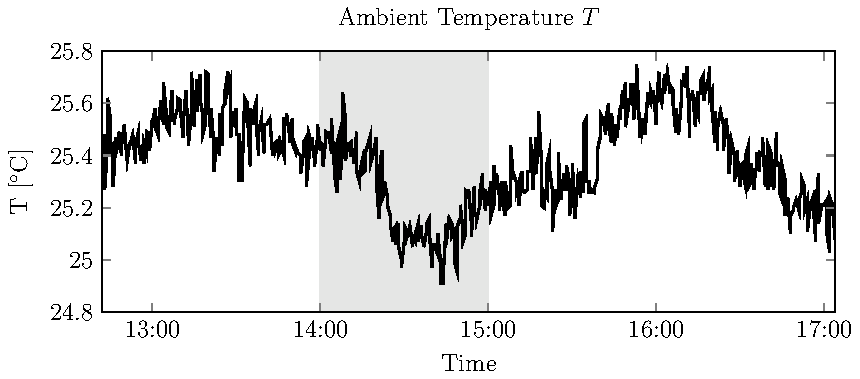
\includegraphics[]{External/PU-temperature.pdf}
  \caption{Ambient temperature $T$ at device for $k = 1000$ BM series over 
  time.  The experiment of 80\% occurred between 14:00 and 15:00 (gray shaded 
area).}\label{fig:PU-temperature}
\end{figure*}

For the three different pulsing frequencies the time difference between the ARF 
and AS of the 100\% duty width measurements for reaching 50\% of the maximal 
value (horizontal dotted lines in \cref{fig:PU-duty-m05}) is $76-57=19[\cdot 
10^{3}\,\sfrac{t}{t_{0}}]$, $88-73=15[\cdot\,10^{3}\,\sfrac{t}{t_{0}}]$, and 
$94-78=16[\cdot\,10^{3}\,\sfrac{t}{t_{0}}]$ for $k=1'000, 5'000,\text{ and } 
10'000$, respectively. This 50\% criteria is the same measure we used in 
\cite{Goering2021} and, in addition, the time differences of the ARF and AS 
have the same magnitudes. However, the time at which the ARF is over 50\% of 
its maximal value is varying for the different $k$ values. Even though we 
limited the changes of the experimental settings between measurement series to 
a minimum, there are slight differences in the amplitude of the incident 
acoustic pressure field which cause these different values of the 50\% 
criteria. This is also the reason why for increasing values of $k$  the start 
time of the AS induced displacement is at a later point in time. In the 
appendix are two additional plots for $\Dy_{i} = \SI{-0.6}{\mm}$ and $\Dy_{i}= 
\SI{-0.4}{\mm}$ that show qualitatively and quantitatively the same behavior 
(\cref{fig:PU-duty-m04,fig:PU-duty-m06}).

For all data series in all three plots, the normalized data is zero for 
$\sfrac{t}{t_{0}}=t\,\fex<0$ (gray shaded area). This is the time span where 
the US excitation is not switched on yet. Since the difference of the averaged 
on data subtracted from the averaged off data is shown and since both have the 
exact same protocol before the US is switched on, this behavior is expected and 
serves as quality control of a data series. A value close to zero after $t>0$ 
indicates that there is no difference in the movement of the particle along 
this direction for a switched on US and a switched off US. When the US is 
switched off, just gravity and the opposite directed buoyancy force are acting 
on the particle because the trapping laser is reduced to such a low laser power 
that the trap exerts negligible forces on the particle.

In addition, for a pulse frequency of $\fp=\sfrac{\fex}{10'000}$ and a duty 
cycle of 50\% the times where the US is switched on and off are visible in the 
data for the ARF (see bottom left plots in
\cref{fig:PU-duty-m04,fig:PU-duty-m05,fig:PU-duty-m06}). This movement resembles an 
upward going staircase and matches the times when the US is switched again on 
after one pulsing period $T_{\mathrm{p}}$. This is in line with the previous 
results from \cite{Goering2021} which showed that the ARF induced movement 
starts immediately as the US is switched on and stops as fast as it started 
when the US is switched off. No such staircase is visible for AS.

Additionally, for all positions $\Dy_{i}$ with a duty percentage of 50\% and a 
pulse frequency of $\fp=\sfrac{\fex}{10`000}$ the final measured value for AS 
is so low and close to zero that it might just be noise and no motion due to 
AS. On the other side, the ARF data for the same data series shows a clear 
displacement of the particle. The reason that we measure for all positions 
$\Dy_{i}$ with 50\% duty percentage and with a pulse frequency of 
$\fp=\sfrac{\fex}{1'000}$ an AS induced displacement is attributed to the 
slight differences in the experimental settings between BM series of different 
values of $k$.

Even though, there are quantitative differences between the different pulse 
frequencies, qualitatively they have the same behavior. In all data series a 
reduced duty percentage is equivalent to a reduced and delayed build up of the 
ARF and AS. Since lower duty percentages lead to less energy in the system, 
this behavior is expected. However, the reduction of the AS build up is more 
than the reduction of the ARF. These different rates of reduction are more 
clearly visible in \cref{fig:PU-all-duty}.

There, the respective last normalized value of a data series of one specific 
duty percentage is plotted versus the duty percentage itself for each 
combination of BM point $\Dy_{i}$ and pulse frequency $\fp$. Each of these 
lines show a linear behavior over all duty percentages. However, the slope for 
the AS data is greater than for the ARF. This linear relation of the ARF for a 
one dimensional standing pressure field to the acoustic energy-density 
$E_{\mathrm{ac}}$ is in line with the theory
\begin{equation*}
  \FARF\propto E_{\mathrm{ac}} \propto p_{a}^{2}
\end{equation*}
where $p_{a}$ is the pressure of the acoustic field 
\cite{Gorkov1962,Bruus2012}. The same linear relation to the acoustic 
energy-density ($\FAS\propto E_{\mathrm{ac}}\propto p_{a}^{2}$) is 
theoretically valid for AS \cite{Bach2020} and also visible here. Nevertheless, 
the here depicted transient behavior of the ARF and AS suggests that the 
interrupted energy supply to the system causes an even further delay of the AS 
build up compared to the ARF build up. The generally lower values for the AS 
induced displacement and also the later start of the AS build up for 
$\fp=\sfrac{\fex}{10'000}$ compared to $\fp=\sfrac{\fex}{1'000}$ is attributed 
to the slight differences in the experimental settings and not a cause of the 
magnitude of $\fp$ itself.

\begin{figure*}[tbp]
  \centering
  % \tikzsetnextfilename{PU-avg-end-over-duty}
{
  \small
%%%%%%%
% READ TABLE
%%%%%%%
\pgfplotstableread{\relPath/10_Figures/TikZ/avg_end_over_duty.dat}{\data}
%%%%%%%
% LINES FOR ALL GROUPPLOTS
%%%%%%%
\begin{tikzpicture}
   \begin{groupplot}[%
       scale only axis,
       group style={
         group size= 2 by 1,
         group name=plots,
         vertical sep=4pt,%
         horizontal sep=20pt},%
       height=35mm,%
       width=64mm,%
       ymin=0, ymax=1.1,
        xticklabel style={
          /pgf/number format/fixed,
          /pgf/number format/precision=2
        }]

%%%%%%
%%% PLOT (1,1)
%%%%%%

   \nextgroupplot[%
      legend style={
        fill=lightgray!90!white,
        font=\footnotesize,
        at={(0.95,0.03)},
        legend columns=3,
        anchor=south east},
      legend cell align={left},
     title={ARF},%
     ylabel style={align=center},
     ylabel={{Normalized\\[-2.5mm] maximal amplitude}},
     xlabel={Duty width [\%]},
 ]

      \addlegendimage{empty legend}
      \addlegendimage{empty legend}
      \addlegendimage{empty legend}

      \addplot[style1000] table[x=duty, y=fp_1000_y] {\data};
      \addplot[style10000] table[x=duty, y=fp_10000_y] {\data};
      \addplot[style5000] table[x=duty, y=fp_5000_y] {\data};

      \addlegendentry{\phantom{a}}
      \addlegendentry{\hspace{-7mm}\textbf{$k$}}
      \addlegendentry{\phantom{a}}
      \addlegendentry{1000};
      \addlegendentry{5000};
      \addlegendentry{10000};


%%%%%%
%%% PLOT (1,2)
%%%%%%

   \nextgroupplot[%
     yticklabels={,,},
     xlabel={Duty width [\%]},
     title={AS},
   ]%

      \addplot[style1000] table[x=duty, y=fp_1000_z] {\data};
      \addplot[style5000] table[x=duty, y=fp_5000_z] {\data};
      \addplot[style10000] table[x=duty, y=fp_10000_z] {\data};

  \end{groupplot}

\end{tikzpicture}
}

  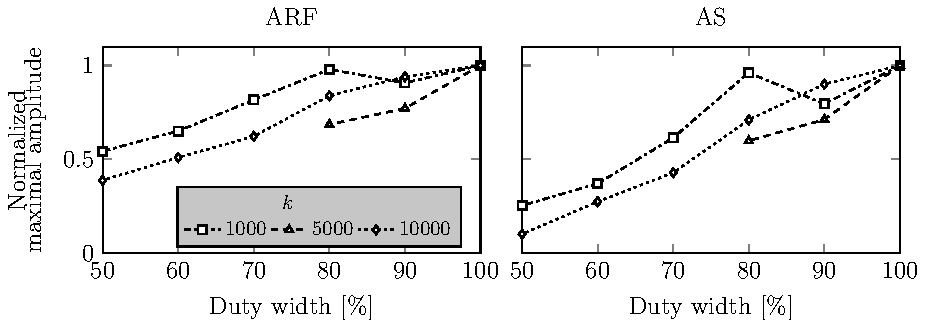
\includegraphics[]{External/PU-avg-end-over-duty.pdf}
  \caption{Final normalized position at end of the build up measurement of 
  $\DV_{y}$ (left column; ARF associated) and $\DV_{z}$ (right column; AS 
  associated) over duty percentage for the three pulsing frequencies 
  $\fp=\sfrac{\fex}{k}$ and averaged over the three locations $\Dy_{i} =
\{\SI{-0.06}{\mm},\SI{-0.05}{\mm},\SI{-0.04}{\mm}\}$. The outlayer for $k=1000$ 
and 80\% duty width is attributed to an unknown external disturbance within the 
OT lab.}\label{fig:PU-all-duty}
\end{figure*}

%%%%%%%%%%%%%%%%%%%%%%%%%%%%%%%%%%%%%%%%%%%%%%%%%%%%%%%%%%%%%%%%%%%%%%%%%%%%%%
%%%%%%%%%%%%%%%%%%%%%%%%%%%%%%%%%%%%%%%%%%%%%%%%%%%%%%%%%%%%%%%%%%%%%%%%%%%%%%
\section{Conclusion}
We extended our previous OT setup to measure the effects of a pulsed ultrasonic 
excitation of a microacoustofluidic system on the build up of the AS and the 
ARF, and also on the final position of a microparticle because of AS and the 
ARF. We varied the pulse frequency $\fp$ and duty width of the pulsed acoustic 
excitation to understand the effects of those parameters on the quantities of 
interest. In addition, we limited the difference of experimental settings 
between measurement series to a minimum for a valid comparison of the data. Our 
results show that the decrease in maximal displacement due to the ARF and the 
drag force from AS are both linear with respect to the applied duty percentage 
and more or less independent of the pulse frequency $\fp$. However, the 
decrease of AS with lower duty percentage is for all BMs faster than for the 
ARF. Even though our BM time span is limited to 120'000 acoustic excitation 
periods $\sfrac{1}{\fex}$ ($\approx$ \SI{96}{\ms}), we still manage to observe 
a significant level of streaming suppression, confirming the experimental 
results of Hoyos and Castro \cite{Castro2016,Hoyos2013}, and paving grounds for 
new theoretical studies that might improve our understanding of the AS build 
up.


% \cleardoublepage
% \include{SECTION/45_Gorkov/gorkov}

\cleardoublepage
\renewcommand{\relPath}{SECTION/50_Viscous_Torque}
 
\chapter[Particle Rotation Measurements with an OT]{Rotational Speed 
Measurements of Small Spherical Particles driven by Acoustic Viscous Torques 
utilizing an Optical Trap}\label{ch:viscoustorque}
\textit{For this work Andreas Lamprecht performed all measurements and sketched 
  a draft for the manuscript. Christoph Goering carried out the postprocessing 
  of the data and the whole submission and writing process.:
\footnote{: DOI: https://doi.org/10.1088/1361-6439/abde92, reproduced with 
permission, copyright 2021 IOP Publishing.}}

\vspace{5mm} \noindent
Andreas Lamprecht, Christoph Goering, Iwan A.T. Schaap, and Jürg Dual,
"Rotational speed measurements of small spherical particles driven by acoustic 
viscous torques utilizing an optical trap", Journal of Micromechanics and 
Microengineering, 2021, \textbf{34} 034004.


\section{Abstract}
Two orthogonal standing acoustic waves, generated by piezoelectric excitation, 
can form a two-dimensional pressure field in microfluidic devices. A phase 
difference of the excitation waves can be employed to rotate spherical 
\si{\micro\meter}-sized silica particles by a torque mediated through the 
viscous boundary $\delta$ around the particle.

The measurement of the rotational rate is, so far, limited to high-speed cameras 
and their frame rate, and gets increasingly difficult when the sphere gets 
smaller.  We report here a new method for measuring the rotational rate of 
\si{\micro\meter} sized spherical particles. We utilize an optical trap with 
high-speed position detection to overcome the frame rate limitation of wide 
field image recording. The power spectrum of an optically trapped, rotating 
particle reveals additional peaks corresponding to the rotational frequencies -- 
compared to a non-rotating particle. We validate our method at low rotational 
rates against high-speed video observation. 

To demonstrate the potential of this method we addressed a recent controversy 
about the rotation of particles with a relatively large VBL 
$\delta$. We measured steady-state rotational rates up to \SI{229}{\hertz} 
(\SI{13.8e3}{\rpm}) for a particle with a radius $R \approx \delta$.  Recent 
numerical research suggests that in this regime the existing theoretical 
approach (valid for $R\gg\delta$) overpredicts the steady-state rotational rate 
by a factor of 10.  With our new method we also confirm the numerical results 
experimentally.

\section{Introduction\label{sec:TC-introduction}}

In recent years, acoustofluidics has provided many powerful tools. Due to being 
contact-less, label-free, and biocompatible 
\cite{Antfolk2015,Abdulla2020,Zielke2020,Binkley2020,Cai2020}, acoustofluidic 
manipulation can be used in medical applications for cancer research
\cite{Antfolk2015,Abdulla2020,Zielke2020,Binkley2020}, Alzheimer research 
\cite{Cai2020}, targeted drug delivery \cite{Bose2015}, and for pumping medical 
fluids \cite{Wu2019}. In addition, there are biological 
\cite{Gerlt2020,Xie2019} and engineering applications (e.g., micro-pumping 
\cite{Wu2019,Huang2014,Lin2019,Ozcelik2021}).

Most of these applications utilize the acoustic radiation force (ARF) to 
manipulate objects on the micro-scale. The ARF is a second-order time-averaged 
effect that arises from the interaction of an acoustic field scattered at an 
object surface and a background acoustic field 
\cite{Doinikov1994Rigid,Hasegawa1969,Yosioka1955,Gorkov1962,Bruus2012}.
These objects can be solid particles, air bubbles, fluid droplets, biological 
samples, as long as their material properties (density $\rho$ and speed of 
sound $c$) are different from the surrounding medium. However, there coexists 
a fluid motion called acoustic streaming (AS) 
\cite{Nyborg1965,Kolb1956,Nyborg1953}. This motion can arise either from
viscous losses in the fluid (Eckhart type streaming \cite{Eckart1948}) or it 
can arise in the viscous boundary layer at a fluid to wall interface 
(Schlichting and Rayleigh streaming \cite{Riley1998,Schlichting1932}).


The theoretical derivations usually describe the steady-state of the AS field. 
A theoretical numerical study \cite{Muller2015} investigated the temporal build 
up of the ARF and AS field. In contrast to the ARF, the viscous drag force 
arising from AS is independent of the object material properties because it is 
a motion of the fluid. The AS direction coincides with the direction of the 
relative motion between fluid and particle.

For a spherical object of radius $R$, the drag force in laminar flow scales 
linearly with the object radius $\FAS \propto R$. In contrast to the $\FAS$, 
the ARF scales with the volume $\FARF \propto \R^{3}$ \cite{Bruus2012-10}.  
Based on the fluid and the object material properties, the $\FARF$ will 
dominate over the $\FAS$ if the radius $\R$ is greater than the critical radius 
$\R_{\text{crit}}$, where $\FAS = \FARF$ holds. The direction of $\FAS$ can be 
different from the $\FARF$. Therefore, the $\FAS$ is usually undesired.

The ARF and the AS occur not only in the bulk of the fluid, but also on sharp 
edges of a device \cite{Doinikov2020a,Doinikov2020b,Leibacher2015,Nama2016}. 
So-called micro-streaming around the surface of a spherical particle can even 
cause a sign inversion of the ARF if the viscous boundary layer $\delta$ is 
sufficiently large \cite{Baasch2019}. However, there are applications that take 
advantage of the AS \cite{Antfolk2014,Mao2017,Hao2020}: a complete overview of 
AS applications can be found in \cite{Wiklund2012a}.

In literature, it is well understood how long it takes until the acoustic 
field, and hence the ARF, needs to build up \cite{Muller2015} and how long the 
particle focusing takes \cite{Bruus2012-10}. However, it is still not fully 
clear how long it takes for the AS to build up, and what the definition for the 
analytical AS time constant is. In the acoustofluidics community, it is 
generally accepted that the build up for the AS field takes longer than the 
build up of the ARF. By using a pulsed actuation of the acoustic field and 
therefore exploiting this time offset, \citeauthor{Hoyos2013} prevented the 
build up of AS \cite{Hoyos2013,Castro2016}. They varied the number of periods 
for which the acoustic actuation is switched on and off, respectively. They 
experimentally showed that for a ratio of about 1 to 1 between 500 on- and 500 
off-periods the streaming velocity is less than 50\% of its steady-state 
magnitude while the ARF is not affected by that much.

\citeauthor{Muller2015} studied the build up of the acoustic energy density and 
streaming velocity with a numerical model \cite{Muller2015}. Their model 
consisted of a fluid cavity without any surrounding structure such as the 
cavity walls. They found numerically that indeed the ARF builds up 
significantly faster than the AS. However, the simulations with a pulsed 
actuation of different ratios of on- to off-periods did not prevent the build 
up of AS because its decay -- as the build up -- is slow compared to the ARF. 
The streaming builds up significantly slower during the on-periods, however, it 
does not decay to its initial value during the off-periods. Over time the 
influence of AS increases because the ARF alternates between some magnitude in 
the on-periods and zero in the off-periods. This implies, that the simulation 
of \citeauthor{Muller2015} could not explain the experimental results by 
\citeauthor{Hoyos2013}.

In this work, we experimentally measure the time until a \Dtwo~spherical 
silicon-dioxide (\SiO) particle moves with constant velocity when accelerated 
by the ARF and AS. Instead of using a camera, we utilize a data acquisition 
board (DAQ) with a sampling frequency of $f_{\text{s}} = \SI{1.25}{\MHz}$ to 
measure the relative particle trajectory as soon as the ultra-sound (US) is 
switched on. This high sampling frequency $f_{\text{s}}$ yields a high 
temporal resolution of $ \Dt = \SI{0.8}{\us}$. Considering the acoustic 
excitation frequency $\fex = \SI{4.015}{\MHz}$, we sample at least every fourth 
excitation period.

The optical tweezer (OT) for this study has already been successfully applied 
in the fields of acoustofluidics for stationary force measurements within a 
microfluidic chip \cite{Lamprecht2016,Lakaemper2015} as well as acoustic 
viscous torque investigations \cite{Lamprecht2021}. Here, we characterize in a 
first step the stationary force field in the bulk of the device to ensure, that 
we measure in a second step the time resolved build up of AS and the ARF 
separately and not their superposition. The separation is done by choosing a 
particle position within the acoustic field, where the $\FAS$ and $\FARF$ are 
orthogonal to each other. In order to measure in the second step solely the 
effects of the acoustic field on the particle and not the characteristics of 
the OT, we alter the usual trapping setup. The modification is that the 
particle is released from the OT before the acoustic excitation starts and 
retrapped after it.  Hence, during the measurement just gravity and the forces 
of the acoustic field act upon the particle. With our modified trapping setup, 
we are able to measure precisely the ARF and AS induced movement of a single 
particle in the bulk of the fluid.

Our manuscript is structured as follows: in \cref{sec:TC-theory} we derive and 
list all time constants in our system and we compute the traveled distances of 
a free floating particle in an acoustic field. Those influences need to be 
considered for our measurement protocol. In addition, we perform numerical AS 
simulations of our device to further understand the AS field; in 
\cref{sec:TC-experimental-setup} we explain our experimental setup and its 
modifications; in \cref{sec:TC-experimental-procedure} we show the results of the 
stationary force measurement, before explaining our time evolution measurement 
protocol and the data post-processing; and in \cref{sec:TC-results} we show and 
discuss the results of this study.




\section{Preliminary Theoretical Considerations\label{sec:theory}}
\subsection{Time Constants}

\begin{figure}[ht]
  \centering
  \def\svgwidth{\figWidth}
  \svginput{\relPath/10_Figures/LaTeX/Device.pdf_tex}
  \caption{Sketch of device. The light-gray area is the silicon channel walls, 
    the light-blue is the fluid cavity, and the dark-gray block the 
    piezoelectric element. The total length of the device is \SI{76}{\mm}. All 
dimensions are as listed in \cref{tab:device-dimensions}.}\label{fig:device}
\end{figure}

\begin{table}
  \centering
  \begin{tabular}{l *{8}{x{10mm}}}
    \toprule
    \toprule
    Symbol & $W$ & $H$ & $W_{D}$ & $H_{T}$ & $H_{B}$ & $l$ & $w$ & $h$ \\
    Value [\si{\milli\meter}] & 3 & 0.1 & 26 & 0.13 & 0.9 & 20 & 4 & 0.5\\
    \bottomrule
    \bottomrule
  \end{tabular}
  \caption{Overview of device dimensions}\label{tab:device-dimensions}
\end{table}


In our experiments there are multiple time constants that need to be considered. 
In the center of interest are the evolution of the ARF and the AS field. The 
acoustic energy $E_{\text{ac}}$, and hence the ARF, has the characteristic 
time constant \cite{Muller2015}
\begin{equation}
    \tarf = \frac{Q}{\omega_{0}} = \frac{Q}{2\pi\,\fex}
  \label{eq:tau-arf}
\end{equation}
with $Q$ being the quality factor of the considered acoustic pressure mode and 
$\fex$ the excitation frequency. For the AS field, a theoretical expression for 
the time constant does not exist. Nevertheless, \citeauthor{Muller2015} report 
a \emph{momentum diffusion time}
\begin{equation}
  \tas = \frac{1}{2\nu}  L^{2} = \frac{\rhof}{2\muef} L^{2}
  \label{eq:tau-nu}
\end{equation}
as the time constant for the AS field. Here, $L$ is half the radius of a 
streaming roll, $\nu=\sfrac{\muef}{\rhof}$ the kinematic viscosity, $\rhof$ the 
density, and $\muef$ the dynamic viscosity of the fluid. This formula is except 
for a factor of $\sfrac{1}{2}$ the same to $\tiner$ (equation 1.88) in 
\cite{Bruus2015}, which is the time a Poisseuille flow needs to fully stop in a 
circular tube of radius $L$ after the immediate removal of its driving 
pressure. To the best of the authors' knowledge, there is so far no better 
approximation for the time constant of the AS field.

When a particle is stably trapped, our OT has the properties of a linear 
mechanical spring \cite{Lamprecht2016}. This spring-like behavior of the OT has 
also a time constant until an acting force moves the trapped particle in its 
equilibrium position. The stiffness of the OT $k_{i}$ is linearly related to a 
characterization parameter of the OT called the cut-off frequency $f_{\text{c}} 
= \sfrac{k_{i}}{2\pi\,\gamma}$ with $\gamma$ being Stokes' drag coefficient 
\cite{Lamprecht2016,Lamprecht2017}. This frequency is the \SI{-3}{\dB} point 
in the Brownian motion power spectrum (more detail in 
\cite{Lakaemper2015,Lamprecht2016}). We can therefore compute the time 
constant of the OT as
\begin{equation}
  \tOT = \frac{1}{2\pi\,f_{c}}.
  \label{eq:tau-OT}
\end{equation}
Lastly, our DAQ system has the time constant $\tqpd$ which describes how fast we 
can measure a sudden change in laser intensity of the OT. This parameter is 
found by changing the laser intensity at a precise point in time and then 
extracting the temporal difference until the DAQ measures it. 

With the parameters of our experiment (see \cref{tab:parameters}) the mentioned 
time constants are as listed in \cref{tab:time-constants}. Hence, with the 
usual trapping mode of the OT, we cannot measure the ARF and AS because $\tOT 
\approx \tas$ and $\tOT\gg\tarf$. In the limit of zero laser power there is no 
trapping potential and hence $\tarf$ and $\tas$ can be measured.

\begin{table}
  \centering
  \begin{tabular}{lccr}
    \toprule
    \toprule
    {\bfseries Parameter} & {\bfseries Symbol} & {\bfseries Value} & {\bfseries 
    Unit}\\
    \midrule
    \textbf{Fluid} & & \\
    Density & $\rhof$ & 1000 & \si{\kg\per\cubic\meter} \\
    Speed of sound & $\cfl$ & 1500 & \si{\m\per\s} \\
    Compressibility & $\kappa_{\text{f}}$ & 4.4E-10 & \si{\per\pascal} \\
    Dynamic viscosity & $\muef$ & 890 & \si{\micro\pascal\second} \\
    Kinematic viscosity & $\nu_{\text{f}}=\sfrac{\muef}{\rhof}$ & 0.890 & 
    \si{\square\mm\per\second} \\
    \midrule
    \textbf{Particle} & & \\
    Density & $\rhop$ & 1850 & \si{\kg\per\cubic\meter} \\
    Radius & $\Rtwo$ & 1.03 & \si{\um}\\
    Radius & $\Rfour$ & 2.195 & \si{\um}\\
    Compressibility & $\kappa_{\text{p}}$ & 1.6E-11 & \si{\per\pascal} \\
    \midrule
    Device quality factor & $Q$ & 36 & - \\
    Corner frequency of OT & $f_{\text{c}}$ & $\approx 100$ & \si{\hertz} \\
    \midrule
    Excitation frequency & $\fex$ & 4.015 & \si{\MHz} \\
    \bottomrule
    \bottomrule
    
  \end{tabular}
  \caption{Symbols and physical properties of the fluid, the particle, and the 
    experimental setup. The quality factor $Q$ is extracted from an admittance 
    measurement of the device filled with water and fixed in the microscope as 
for all measurements. The magnitude of $f_{\text{c}}$ is the usual value in 
stationary force measurements for the OT.}\label{tab:parameters}
\end{table}

\begin{table}
  \centering
  \begin{tabular}{l S[table-format=7.5]S[table-format=7.1]}
    \toprule
    \toprule
    {\bfseries Symbol} & {\bfseries $\tau_{i}$ [\si{\ms}]} & {\bfseries 
    $\sfrac{\tau_{i}}{t_{0}}$ [-]}  \\
    \midrule
    $\tOT$ & 1.59 & 6383.9 \\
    $\tqpd$ & 0.050 & 200.8 \\
    $\tarf$ & 0.0014 & 5.6 \\
    $\tas\vert_{L=\sfrac{H}{2}}$ & 1.44 & 5781.6\\
    $\tas\vert_{L=\sfrac{H}{4}}$ & 0.35 & 1405.3\\
    $\tdrag$ & 0.00049 & 2.0 \\
    \midrule
    $\Dt_{\text{DAQ}}$ & 0.0008 & 3.2 \\
    \bottomrule
    \bottomrule
    
  \end{tabular}
  \caption{Overview of time constants $\tau_{\text{i}}$ for the system. The 
    values are obtained by using the values from \cref{tab:parameters} and 
    \cref{eq:tau-nu,eq:tau-arf,eq:tau-OT,eq:tau-drag}. $\tqpd$ is measured, 
    $\Dt_{\text{DAQ}} = \sfrac{1}{f_{\text{s}}}$, and 
$t_{0}=\sfrac{1}{\fex}$.}\label{tab:time-constants}
\end{table}

\subsection{Free Particle Motion}

If there is no trapping laser power, the spherical particle with mass $m$ will 
move in the fluid due to some acting force $F$; this force can be gravity, the 
ARF, the drag force from AS, or a combination of them. The one dimensional 
dynamic equation for the particle displacement $q$ far away from any walls is 
the same for the three spatial directions $\ex, \ey$ and $\ez$.
\begin{equation}
  \ddot{q} = - \frac{F}{m} - \frac{\gamma}{m}\,\dot{q} =
  - \tilde{F} - \frac{1}{\tdrag}\,\dot{q}
  \label{eq:free-fall}
\end{equation}
with $F$ being a force acting along the direction of $q$ and
\begin{equation}
  \tdrag = \frac{m}{\gamma} = \frac{V\,\rhop}{6\pi\,\R\,\muef}
  = \frac{2}{9}\,\R^{2}\,\frac{\rhop}{\muef}.
  \label{eq:tau-drag}
\end{equation}
Here, $\R$ is the particle radius, $V$ the particle volume, and $\rhop$ the 
particle density. In microfluidics the viscous effects dominate over the 
inertial effects \cite{Bruus2015}. Therefore, we neglect $\ddot{q}$ for further 
calculations. Solving the modified first order ordinary differential equation
\begin{equation}
    \dot{q}= - \tdrag\,\tilde{F} = -\frac{F}{m}\,\tdrag
  \label{eq:mod-free-fall}
\end{equation}
with the initial condition $q\vert_{t=0} = 0$, gives the linear relation $q(t) 
= - \tdrag\,\tilde{F}\,t$ with the integration constant being zero.

As already mentioned, we measure while there is no trapping potential of the 
OT. Therefore, on the particle act only gravity and the forces from the 
acoustic field. In our experiment we have for $F$ along $\ey$ a spatially 
varying force with a maximal value of \SI{0.5}{\pico\newton} and along $\ez$ 
the buoyancy corrected gravitational force $\tilde{m}g=V\,\left( \rhop-\rhof 
\right)\,g$ with a magnitude of \SI{38.2}{\femto\newton} and an acoustic force 
with a maximal value of \SI{0.25}{\pico\newton} (for acoustic force magnitudes 
see \cref{fig:2um_map}). As we will explain later (see 
\cref{sec:experimental-procedure}), we have \SI{25}{\ms} without any laser 
power where the particle will solely move due to gravity and then \SI{30}{\ms} 
of US excitation where also the acoustic forces are acting.

Hence, a spherical \SiO~$\Rtwo=\SI{1.03}{\um}$~particle will have moved 
$0\Rtwo$ along $\ey$ and $0.05\Rtwo$ along $\ez$ after $\SI{25}{\ms}$ with just 
gravity acting. And, after $\SI{55}{\ms}$, when there are additionally 
constant acoustic forces, the particle will have traveled distances of 
$0.84\Rtwo$ and $0.54\Rtwo$ along $\ey$ and $\ez$, respectively. For the 
latter, $0.54\Rtwo$ is the sum of $0.12\Rtwo$ due to gravity and $0.42\Rtwo$ 
due the force from the acoustic field.

\subsection{Numerical Streaming Simulations}

To understand the influences and implications of the AS on our measurements, we 
simulate with {\ttfamily COMSOL Multiphysics 5.6} (COMSOL Inc., Stockholm, 
Sweden) 2 two-dimensional structures that relate to the experimental device; 
one with just the fluid cavity as the baseline model (cavity-only model); and 
the other with added structure around the cavity to reflect our real device 
(whole-device model). See \cite{supplemental} for both models as one {\ttfamily 
.mph} file. For both we follow the work of \citeauthor{Muller2015} 
\cite{Muller2015} in terms of the fluid mesh size.

\afterpage{
  \vspace*{\fill}
\begin{figure}[H]
  \centering
  \begin{subfigure}{\figWidthDouble}
    \centering
      \caption{Streaming simulation for cavity-only model at $f_{\text{max}} = 
      \SI{3.987}{\MHz}$.}\label{subfig:JC-streamingrolls}
    \def\svgwidth{\figWidthDouble}
    \textsf{\tiny % that is for the added unit @ the axis
    % \input{10_Figures/LaTeX/JC-streaming-rolls.pdf_tex}
    \svginput{\relPath/10_Figures/LaTeX/JC-streaming-rolls_paraview.pdf_tex}}
    \end{subfigure}\\%k
  \begin{subfigure}{\figWidthDouble}
    \centering
    \caption{Streaming simulation for whole-device model at $f_{\text{max}} = 
    \SI{3.745}{\MHz}$. The gray area is the structure around the 
  cavity.} \label{subfig:FD-streamingrolls}
    \def\svgwidth{\figWidthDouble}
    \textsf{\tiny % that is for the added unit @ the axis
    \svginput{\relPath/10_Figures/LaTeX/FD-streaming-rolls_paraview.pdf_tex}}
    % \input{10_Figures/LaTeX/FD-streaming-rolls.pdf_tex}
  \end{subfigure}
  \caption{Results for streaming simulations of a cavity-only model (a) and a 
    model with surrounding structure (b). The colormap shows the total acoustic 
    pressure and the white arrows the streaming flow. For both simulations 
    $f_{\text{max}}$ is the frequency of maximal acoustic energy density 
    $E_{\text{ac}}$ for a pressure mode with 16 nodal lines. The pressure mode 
  for both simulations is the same besides the phase shift of 
$\pi$.}\label{fig:comsol-streaming}
\end{figure}
\vspace*{\fill}
  \clearpage
}

We model a two-dimensional $yz$ slice of the whole device as seen in 
\cref{fig:device} without the piezoelectric transducer (PZT) and its glue 
layer. Therefore this whole-device model consists of two glass, two silicon, 
and one water domain. We utilize the Solid Mechanics \comsol{solid} interface 
for the silicon and glass. For the cavity we employ the Creeping Flow 
\comsol{spf} interface with the spatial variation of the Reynolds Stress as 
source and the Stokes drift as the boundary condition. Also in the cavity, we 
use the Thermoviscous Acoustics \comsol{ta} interface. Lastly, we couple the 
Solid Mechanics with the Thermoviscous Acoustics via Thermoviscous 
Acoustic-structure Boundary \comsol{tsb}. The cavity-only model solely needs 
the Creeping Flow and the Thermoviscous Acoustics interface without 
multiphysics coupling.

Besides the added structure around the cavity, the main difference between the 
two models is the location of the excitation. The whole-device model has as 
boundary condition a prescribed displacement along $\ez$ of 
$z_{\text{BD}}=\SI{0.1}{\nm}$, where the PZT is glued onto the device. The 
cavity-only model, however, has a prescribed constant velocity of its left 
cavity wall along $\ey$ of $\dot{y}_{\text{BD}} = \SI{25}{\mm\per\second}$. 
This magnitude corresponds to the mean wall velocity of the whole-device model, 
where the excitation is at the PZT. With those two boundary conditions the 
acoustic pressure is \SI{310}{\kPa} for the whole-model and \SI{550}{\kPa} for 
the cavity-only model at their respective 16 nodal pressure line frequency with 
maximal acoustic energy density $E_{\text{ac}}$. The discrepancy in pressure 
amplitude comes from the applied boundary conditions of respective models.

The respective frequencies of maximal $E_{\text{ac}}$ 
(\SI{3.9876}{\MHz} and \SI{3.7450}{\MHz}) inside the cavity while having a 16 
nodal line mode were determined with a frequency sweep. This is the same mode 
we have in our experiment as well. For the streaming simulation, we employ a 
stationary study of the Creeping Flow interface that uses the results from the 
frequency domain study in its source term and as the boundary conditions.

\Cref{fig:comsol-streaming} shows the results for the pressure and streaming 
fields of both models. The magnifications correspond to the area where we 
perform our measurements in the experiment. One can see that the simulated 
pressure fields are qualitatively the same, however, the streaming fields 
differ to a great extent. The cavity-only simulation depicts spatially 
repetitive streaming rolls over the whole fluid domain. In the bulk of the 
fluid is Rayleigh streaming. However, near-boundary Schlichting streaming is 
not visible because the viscous boundary layer is relatively small. In contrast 
to that, the simulation for the whole-device model has a non-spatially 
repetitive streaming field. There are regions where its similar to the 
cavity-only model streaming field. But, the streaming pattern is non-repetitive 
and exhibits strong local differences. As a consequence, care must be taken to 
chose a measuring point where the $\FAS$ and $\FARF$ are orthogonal to each 
other to ensure no superposition of forces.

Although the clamping of the microscope setup and the oil immersion layer for 
the lens are excluded in the model with structure, one can see that the 
streaming field is a local, non-periodic effect, whereas the pressure field is 
spatially periodic. We expect that these tendencies remain the same when the 
clamping, the immersion layer, and the PZT are added.

\section{Experimental Set-up\label{sec:VT-experimentalSetUp}}
\subsection{Optical Trap\label{sec:VT-opticalTrap}}

The optical trap is based on the apparatus described in detail elsewhere 
\cite{Bodensiek}. We modified and enhanced the standard setup and its 
peripherals such that it is suitable for our micro-fluidic applications. These 
applications require a long term laser stability, fine spatial resolution in 
three dimensions, spatial reproducibility of the positioning system, and fine 
temporal resolution of the DAQ system. The taken measures are explained in the 
following.

The collimated beam of a \SI{200}{\milli\watt} (lineary polarized in the 
$yz$-plane, $<$0.5\% power drift in \SI{8}{\hour}), \SI{785}{\nano\meter} near 
infrared laser diode (LuxX 785-200, Omicron Laserprodukte GmbH, 
Rodgau-Dudenhofen, Germany) is coupled into a standard microscope chassis (Nikon 
NI-U, Tokyo, Japan).  Although the laser is linearly polarized, it forms a 
symmetric optical trapping potential by focusing the laser beam with a water 
immersion microscope objective (CFI Plan Apo IR SR 60XWI 1.27NA, Nikon, Japan) 
with a high numerical aperture (NA) of 1.27. Immersol W with a refractive index 
of $n=1.33$ at room temperature (Zeiss, Germany) is used as an immersion media 
instead of water to obtain a higher temporal stability of acoustic standing wave 
modes during the experiments \cite{Lamprecht2016}.  Downstream of the focused 
laser beam, the laser light is collimated again by an air condenser (C-C Abbe NA 
0.9, Nikon, Japan) and split into two separate beams by a non-polarizing 50:50 
beam splitter (CCM1, Thorlabs, USA). A schematic sketch of the optical set-up 
and the focused laser inside an acoustofluidic flow cell is shown in 
\cref{fig:Fig2}.

%%%%%%%%%%%%%%%%%%%
\begin{figure}[tb]
    \centering
    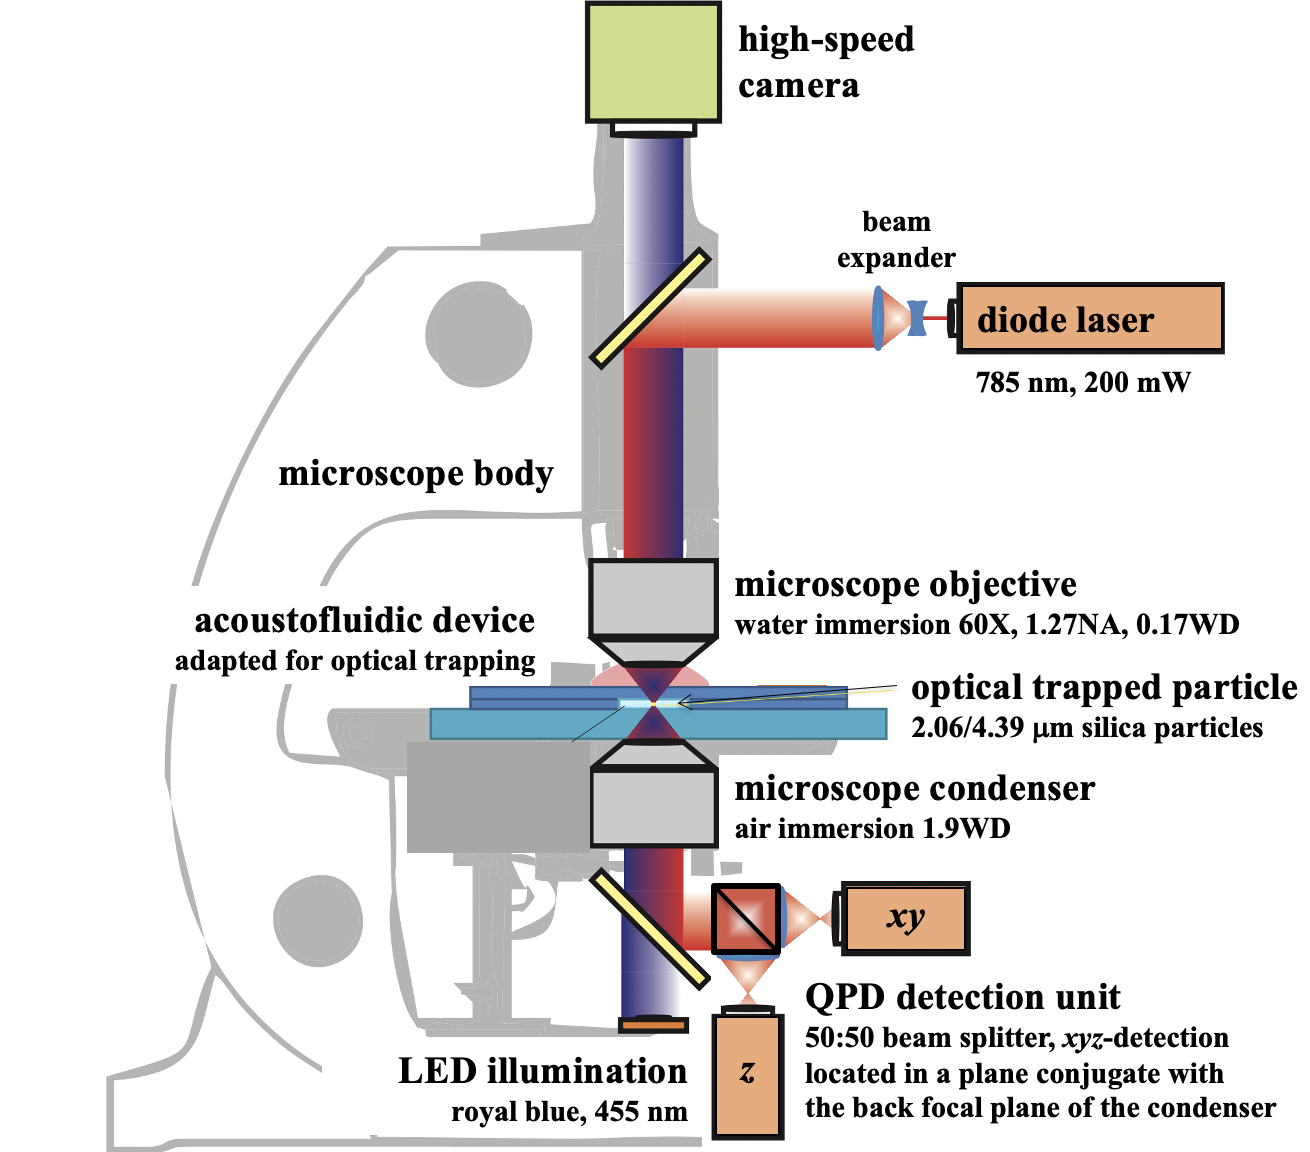
\includegraphics[width=84mm]{Fig2.png}
    \caption{The optical trap is based on a commercial upright microscope body.  
        The linear polarized laser light (\SI{785}{\nano\meter}) is aligned on 
        an optical table and coupled into the microscope. The microscope 
        objective forms the laser focus for trapping, and the condenser directs 
    the laser light to the detection unit, where QPDs are used for the analysis 
  of the particle displacements. An LED illuminates the sample and a high-speed 
camera is used for imaging.\label{fig:Fig2}}
\end{figure}%
%%%%%%%%%%%%%%%%%%%

The laser beam is projected onto a Quadrant Photo Detector (QPD) that is 
conjugated with the back focal plane of the condenser \cite{Bodensiek}. The 
QPD-$xy$ in \cref{fig:Fig2} is optimized to detect the $xy$-displacement of 
optically trapped particles. The laser spot size on the QPD-$xy$ is about 
\SI{2}{\mm} in diameter and the \SI{8}{\mm} diameter sensor measures 
displacements of the beam in the back focal plane. The QPD-$z$ measures the 
total laser intensity over its four quadrants which scales with the 
z-displacement of the particle inside its optical potential \cite{Dreyer}.

The analog data of the QPDs is anti-aliasing filtered at \SI{15}{\kilo\hertz} 
and is digitized by a data acquisition board (NI USB-6356, National Instruments, 
Austin, TX, US) with a sampling frequency of \SI{1}{\MS} (1 million samples per 
second). We recorded the Brownian motion of the particle within the optical trap 
for ten seconds and then performed a Fast Fourier Transform (FFT) on this signal 
to achieve a frequency resolution of $\Delta f=\SI{0.1}{\hertz}$. This spectrum 
is averaged over 10 cycles such that the calibration takes \SI{100}{\second}.  
The recorded signals are then further processed for calibration and force 
measurements in 3D with a self-written Matlab and LabVIEW (National Instruments, 
Austin, TX, US) routine.  Calibration of the position (\si{\meter\per\volt}) and 
force sensitivity (\si{\newton\per\meter}) was obtained via the Equipartition 
Theorem \cite{Svoboda,Vermeulen}. These calibrations are performed for the $x$-, 
$y$- and $z$-directions simultaneously. Due to the elongated shape of the focal 
spot in the $z$-direction, the optical trap stiffness $\kappa_z$ is 3 to 5 times 
weaker than the trapping stiffness in $x$- and $y$-direction. 

Here, a typical optical trapping stiffness for \SI{100}{\milli\watt} laser power 
and \SI{2.06}{\micro\meter} silica particles is 
\SI{2.9}{\femto\newton\per\micro\meter} in the $xy$-plane and 
\SI{1.1}{\femto\newton\per\micro\meter} in the $z$-direction. During the 
experiments it was ensured with the magnitude of the laser power that the 
displacements $u$ of the particles remained inside the valid regime of the trap 
calibration ($u<\sfrac{R}{2}$). The main counteracting force is the acoustic 
radiation force. With our Optical Trap setup we can stably trap particles 
between \SI{2}{\micro\meter} to \SI{10}{\micro\meter}. Larger particles tend to 
show unstable trapping in our setup.
% unstable trapping in our setup; smaller particles get closer to the used laser 
% wavelength ($\lambda = \SI{785}{\nano\meter}$) whereas our calibration method is 
% derived for $\lambda < R_{\text{particle}}$.

The spatial positioning of the optical trap in the $xy$-direction and 
$z$-direction was performed by a closed-loop motorized microscope stage (SCAN, 
Marzhauser, Wetzlar, Germany) and closed-loop piezo stage (PI, P-725.2CD, 
Karlsruhe, Germany), respectively. The statistic force repeatability of the 
optical trapping set-up was $\pm \SI{11}{\femto\newton}$ \cite{Lamprecht2016}, 
which includes positional drifts and eventual variations in temperature.

\subsection{Acoustofluidic Flow Cell\label{sec:VT-DeviceAndAcoustics}}

Within the optical trap, the working distance of the microscope objective 
(\SI{0.17}{\milli\meter}) and of the condenser (\SI{1.9}{\milli\meter}) limits 
the thickness of the flow cell.  Furthermore, the device has to be transparent 
for the laser wavelength $\lambda$ to permit optical trapping and detection (see 
\cref{fig:Fig2}). Therefore, a transparent glass device was built from a stack 
of standardized microscope coverslips (MENZEL GmbH, Braunschweig, Germany). It 
was designed to excite two individual standing waves in $x$- and $y$-direction 
separately, which provide the necessary conditions to rotate spherical 
\si{\micro\meter} particles. 

Similar as in \citeauthor{Lakamper} \cite{Lakamper}, a polyurethane spray glue 
(ITW, Cramolin Urethan, Muehlacker, Germany) was used for the fabrication of the 
micro-fluidic flow cells. Two square shaped coverslips of size (thickness, 
\numrange{0.13}{0.17} \si{\milli\meter}, and \SI{22x22}{\mm} large) were glued 
together and afterwards a \SI{4.0}{\milli\meter} wide cross-shaped fluid channel 
was diced into the center of one of the two coverslips. The remaining material 
of the diced coverslip was covered by another adhesive layer and glued onto a 
rectangular glass (thickness, \numrange{0.13}{0.17} \si{\milli\meter}, 
\SI{60}{\mm} long, \SI{22}{\mm} wide). The resulting stack of coverslips formed 
two crossed fluid channels in $x$- and $y$-direction with open ends (soft 
acoustic boundaries). The maximal distance of the fluid cavity depth plus the 
top cover thickness is $< \SI{270}{\micro\meter}$ as depicted in 
\cref{fig:Fig3}. An adapted phenolic paper with the size of a standard specimen 
slide ($l$, $w$, and $h$ = \numlist{75; 25; 1} \si{\mm}) holds the stacks of 
coverslips, so that the acoustic flow cell can be easily placed in the sample 
holder of the microscope stage.

%%%%%%%%%%%%%%%%%%%
\begin{figure}
    \centering
    \includegraphics[width=84mm]{Fig3.png}
    \caption{Stack of three coverslips form the device where the middle layer 
    includes two fluid channels (\SI{4.0x22}{\mm} with a depth of 
    \numrange{0.13}{0.17} \si{\milli\meter}, red boxes) in an orthogonal 
    arrangement. The two channels intersect and form a \SI{4.0x4.0}{\mm} crossed 
    chamber (black hatched area). Each piezo-electric transducer 
    \SI{4.0x2.0x0.5}{\mm} (PZ26, blue boxes) individually excites a direction.  
    The relative phase difference $\zeta$ of the excitation signals is freely 
    adjustable. The phenolic paper holds the stack and has the size of a 
    standard specimen slide for mounting.\label{fig:Fig3}}
\end{figure}
%%%%%%%%%%%%%%%%%%%

Two piezo-electric transducers (Ferroperm, Pz26, $l$, $w$, and $h$ = \numlist{4; 
2; 1} \si{\mm}, Kvistgaard, Denmark) were glued on the stack of coverslips with 
conductive glue (EPOXY Technology, H20E, Billerica, MA, USA) perpendicular to 
each channel in $x$- and $y$-direction. The distance between the center of the 
fluidic chamber and each transducer was \SI{7}{\mm}. This distance was set such, 
that the microscope objective stays clear from the transducers. The resulting 
thin design of the device ensured the usage of the optical trap and decoupled 
the standing wave modes in the channels ($x$ and $y$). This specific design 
enabled controlled excitation of standing wave modes in the directions of $x$ 
and $y$ as well as an individual control of the excitation phase $\zeta$ (see 
\cref{fig:Fig4}).

For our measurements we always used the same spatial position within the device.  
Hence, the rotation of the particles is always in the same direction for our 
experiments. However, \citeauthor{lamprecht2015} \cite{lamprecht2015} 
demonstrated how the rotation direction is dependent on the spatial location and 
the phase $\zeta$ of the two standing waves. In addition, in the supplemental 
material two videos are provided that show the change of rotation direction when 
changing these two parameters.

%%%%%%%%%%%%%%%%%%%
\begin{figure}
    \centering
    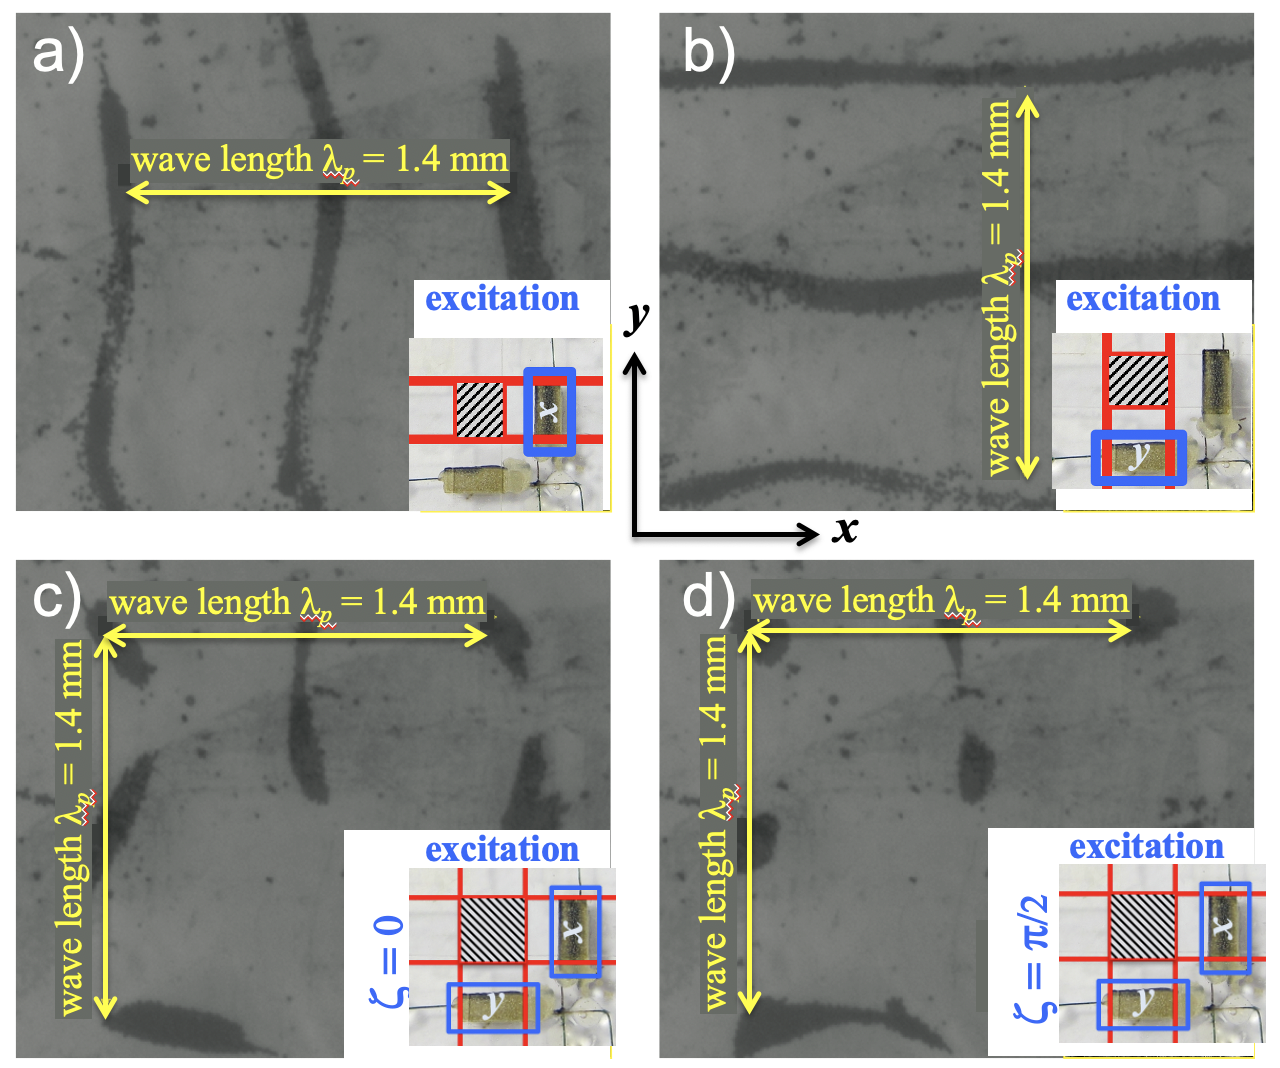
\includegraphics[width=84mm]{Fig4.png}
    \caption{The device is filled with a water/glycerol (70$\%$/30$\%$) mixture 
    containing \SI{4}{\micro\meter} copolymer particles (Duke Scientific 
    Cooperation, Palo Alto, CA, USA) and it has two identical modes in $x$- and 
    $y$-direction at \SI{1.043}{\mega\hertz}. a) and b) depict the isolated 
    modes at \SI{15}{\Vrms} for the $x$- and $y$-direction, respectively. The 
    resulting measured wavelength $\lambda_{P}$ was approximately 
    \SI{1.4}{\milli\meter} for both directions.\ c) and d) show the particle 
    pattern for the two orthogonal standing waves inside the crossed-fluid 
    chamber at $\zeta= 0$ and $\zeta= \frac{\pi}{2}$, respectively. These 
    observations confirm the assumption of a 2 dimensional orthogonal standing 
    wave field.\label{fig:Fig4}}
\end{figure}
%%%%%%%%%%%%%%%%%%%


\subsection{Particles \label{sec:VT-particles}}
For the visualization experiment in \cref{fig:Fig4} we used \SI{4}{\micro\meter} 
copolymer particles (Duke Scientific Cooperation, Palo Alto, CA, USA). For the 
optical trapping experiments with single particles we used silica particles 
because they are more precise in their dimensions compared to polystyrene 
particles. In addition, they have better interactions
with the acoustical field. Moreover, the results of \citeauthor{hahn2016} 
\cite{hahn2016} suggest that in the region of $R \approx \delta$ and ratios of 
$\sfrac{\rho_{\text{s}}}{\rho_{\text{f}}}$ between 2 and 15 result a greater 
magnitude of the acoustic viscous torque results. With the used fluid ($\rho_{f} 
= \SI{1.1}{\gram\per\cubic\centi\meter}$) and our silica particles ($\rho_{s} = 
\SI{2.0}{\gram\per\cubic\centi\meter}$) the ratio 
$\sfrac{\rho_{\text{s}}}{\rho_{\text{f}}} \approx 1.8$.

In order to validate the proposed power spectrum method two sets of validation 
experiments are explained in \cref{sec:VT-rotationDetectionValidation}. For those 
the \SI{4.39}{\micro\meter} particles were modified differently for each 
experiment. We use this size of particles since they are better visible when 
simultaneously measuring the rotation with a camera. There was the need to 
\emph{mark} the spherical \SI{4.39}{\micro\meter} silica particles because a 
reliable rotation measurement with the camera of unmarked spherical particles 
was not possible.

Two methods for marking were used. In both cases the rotation could be easily 
tracked by optical microscopy because the particle size of 
\SI{4.39}{\micro\meter} silica glass micro-spheres (Microparticles
GmbH, Berlin, Germany) is much larger than the optical resolution.
For the set of experiments, silica particles were deformed between two polished 
metal plates by applying a pressure of \SI{1}{\mega\pascal} to achieve a slight 
degree of non-sphericalness (see \cref{fig:Fig5}). For the second set, uncoated 
particles were distributed on a glass specimen slide (MENZEL GmbH, 
Menzel-Glaesser, Braunschweig, Germany) and coated by a Sputter coater (B7340 
Manual Sputter Coater, Van Loenen Instruments, Zaandam, Netherlands) with a gold 
coating (see \cref{fig:Fig6}). After coating, the particles were half-covered 
with a \SIrange{10}{20}{\nano\meter} thick gold layer at their surface 
orientated to the gold electrode. The coating affected the acoustic properties 
not substantially. The particles showed, i.e., same trapping and rotational 
behavior within the acoustical trap. Averted particle surfaces showed a thinner 
gold layer of about \SIrange{0}{10}{\nano\meter}.

\section{Experimental Procedure\label{sec:VT-experimentalProcedure}}

The observed time-averaged spatial off-set of the particles inside the optical 
trap is naturally zero, but the frequency content of the observed particle 
motion includes the thermal energy content of the particle as well as its 
rotational frequency. The angular frequency appears as an additional peak in the 
power spectrum of the rotating particle. In order to validate this detection 
method, particles with a rotational rate of less than \SI{1.66}{\hertz} 
(\SI{100}{\rpm}) were observed by a high-speed camera (HiSpec1 G2 Mono, Fastec, 
San Diego, USA) while also recording their power spectrum.  In the validation 
experiments the transparent device was filled with \SI{4.39}{\micro\meter} 
silica glass micro-spheres suspended in distilled water at a low concentration 
of a few particles per \si{\micro\liter}.  This low particle concentration does 
not effect the ratio $\tilde{\rho} = \sfrac{\rho_{\text{s}}}{\rho_{\text{f}}}$. 
The open channel ends were sealed with silicone oil to ensure a constant fluid 
volume during the measurements.

\subsection{Rotation Detection 
Validation\label{sec:VT-rotationDetectionValidation}}

Two sets of validation experiments were performed: (i) non-spherical particle 
rotation with slightly non-spherical particles; (ii) spherical particle rotation 
with gold covered particles for increased contrast in the video observation 
\cite{Lamprecht2013}. 

According to \citeauthor{Hahn2016} \cite{Hahn2016}, non-spherical objects can 
also be rotated due to the acoustic VT, but here effects of acoustic radiation 
torques may govern or influence their rotations \cite{Wang2012}. A slightly 
non-spherical \SI{4.39}{\micro\meter} silica particle (see \cref{fig:VT-Fig5}) was 
trapped in the optical potential well with \SI{100}{\milli\watt} laser power and 
moved to the reference position ($x,y,z = 0$) in the center of all three 
dimensions of the fluid chamber. The acoustic pressure field is formed by two 
orthogonal standing waves at the same excitation frequency of 
\SI{1090}{\kilo\hertz} and \SI{10.0}{\Vrms} amplitude. The particle was then 
optically moved to the closest resulting pressure node (intersection of two 
pressure nodal lines in $x$- and $y$-direction) with respect to the reference 
position. Positions of the pressure nodes were determined by a previous set of 
experiments.

The phase difference between the acoustic excitation directions $x$- and 
$y$-direction was set to $\zeta=\sfrac{\pi}{2}$, and the non-spherical particle 
rotated counter-clockwise with $\Omega = \SI{1.12}{\hertz}\,(\SI{67}{\rpm})$ 
(arithmetic mean of \SI{0.3}{\hertz} (\SI{18}{\rpm}) and \SI{1.6}{\hertz} 
(\SI{96}{\rpm}); see also \cref{fig:VT-Fig5}). At $\zeta=0$ the particle did not 
rotate because of the stable, non-varying acoustic potential.

%%%%%%%%%%%%%%%%%%%
\begin{figure}
    \centering
    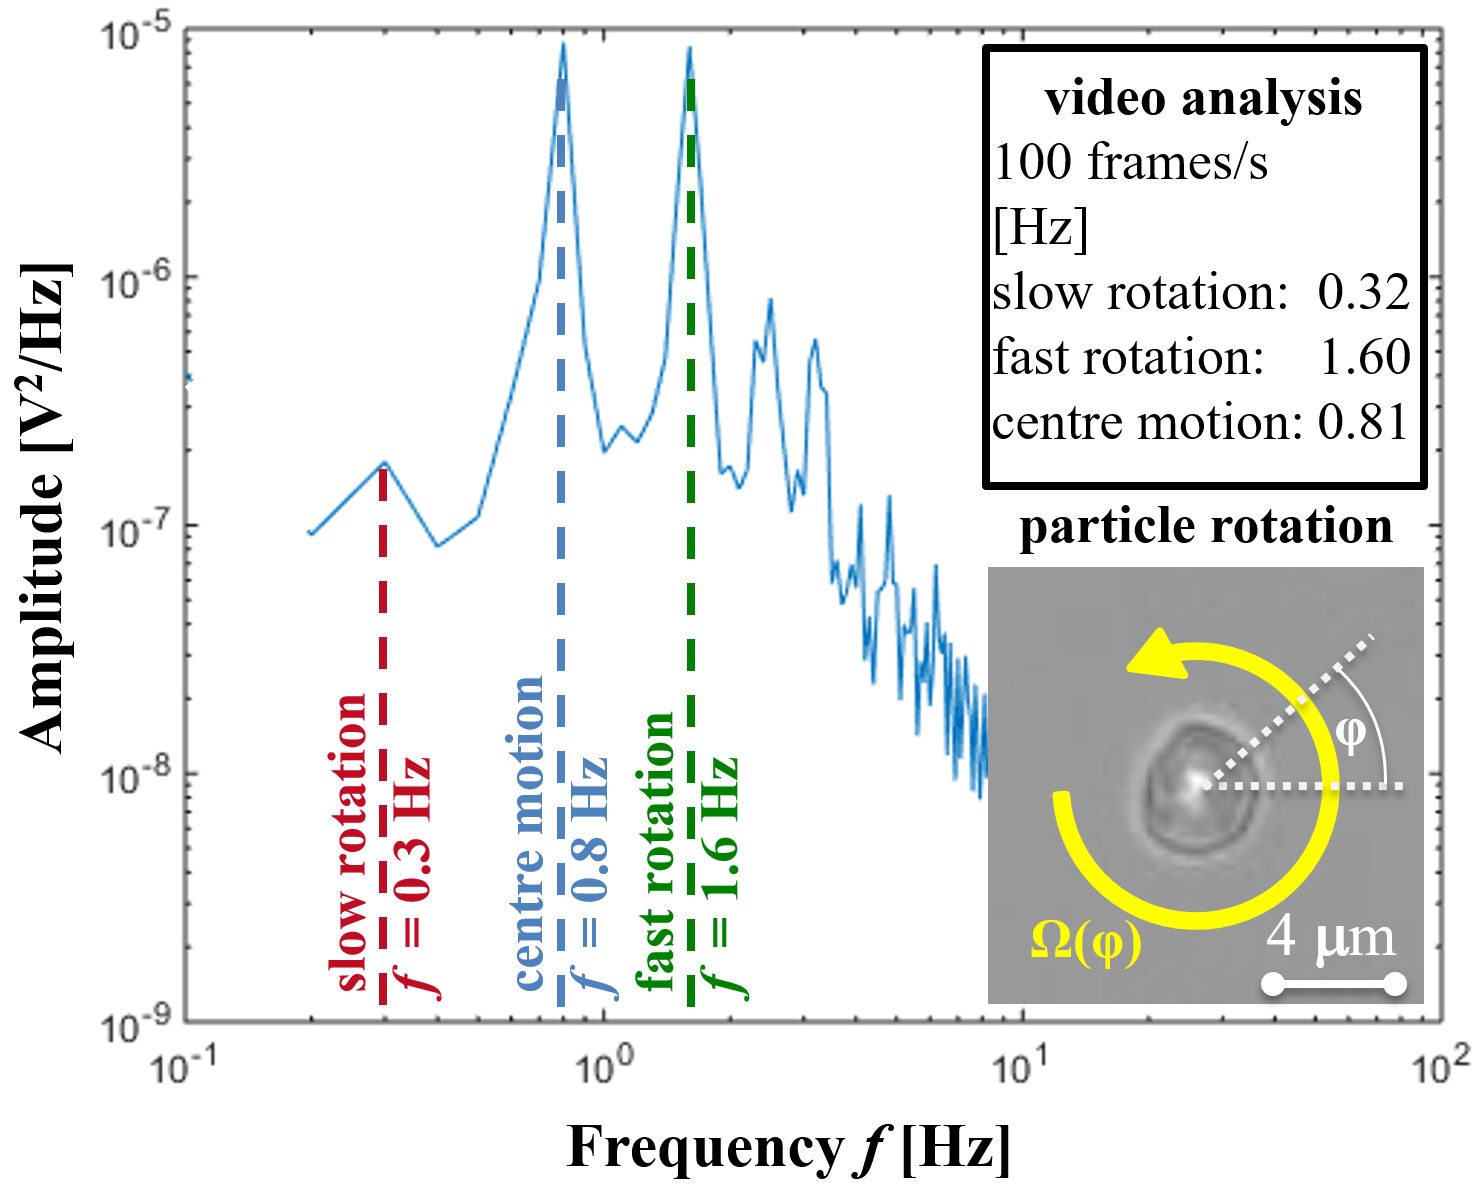
\includegraphics[width=100mm]{\relPath/10_Figures/Fig5.png}
    \caption{Power spectral density and results of the video analysis of a 
      counter-clockwise rotating non-spherical silica particle at 
      \SI{1090}{\kilo\hertz} and \SI{10.0}{\Vrms} with relative phase shift of 
      $\zeta= \sfrac{\pi}{2}$. The 10 times averaged power spectrum of the 
      $y$-signal of the detection unit (QPD) was recorded with a frequency 
      resolution of $\Delta f = \SI{0.1}{\hertz}$ and a sampling rate of 
      \SI{1}{\MS}. Three main peaks were observed at \numlist{0.3; 0.8; 1.6} 
      \si{\hertz}. The frequency peak at \SI{0.8}{\hertz} corresponds to a 
      relative $xy$-motion of the trapped particle, whereas the peaks at 
      \numlist{0.3; 1.6} \si{\hertz} (\numlist{18;96} \si{\rpm}) are related to 
      a non-constant angular rotation $\Omega(\varphi)$ of the particle. The 
      measured results are in correlation with the determined rotational rate by 
      the high-speed video analysis with a frame rate of \SI{100}{\fps}. See the 
      supplemental material for a optically trapped particle rotating 
      sequentially with two velocities due to its imperfect spherical 
  shape.\label{fig:VT-Fig5}}
\end{figure}%
%%%%%%%%%%%%%%%%%%%

In \cref{fig:VT-Fig5}, the average of 10 power spectral density plots is depicted, 
each obtained from a \SI{10}{\second} recording. The frequency resolution is 
$\Delta f=\SI{0.1}{\hertz}$. Three main peaks were observed in the power 
spectrum at \numlist{0.3; 0.8; 1.6} \si{\hertz}, which correlate with the 
frequencies detected by the contemporaneous video detection. We see these peaks 
on both QPDs for the $x-$ and $y$-direction. However for some of the latter 
rotational measurements, the $xy$-motion of the particle adds more peaks 
depending on the major axis of the acoustic displacement. All other peaks are 
related to multiple repetitions of these angular frequencies due to deviations 
of the spherical shape of the particle.  The peak at \SI{0.8}{\hertz} 
corresponds to a relative $xy$-motion of the particle, whereas the peaks at 
\numlist{0.3; 1.6} \si{\hertz} are related to angular frequencies of the 
non-constant rotation $\Omega(\varphi)$ of the particle. The existence of two 
frequency peaks is related to the influence of different acoustic pressures in 
$x$ and $y$-direction because the amplitude were not yet matched for this 
validation.  Hence, the acoustic radiation forces on the particle have different 
magnitudes in $x$ and $y$-direction. So, the distribution of acoustic radiation 
pressure on the particle changes during its rotation and leads to an additional 
orientation dependent acoustic radiation torque.  The influence of acoustic 
radiation forces on particle orientations is a well-known effect for small 
non-spherical particles with $r \ll \lambda$ \cite{Konig1891,Garbin2015}, but 
this experiment shows that this influence is also large enough to influence the 
rotation by the acoustic VT.  Particles with a larger degree of 
non-sphericalness did not even start to rotate in this set of experiments. This 
is in agreement with the predictions of \citeauthor{Hahn2016} \cite{Hahn2016}, 
that the acoustic VT decreases with a higher degree of elliptical shape of the 
particles. In contrast, the acoustic radiation torque increases and hinders a 
constant rotation of the particle, if the symmetry of the experimental acoustic 
potential at $\zeta= \sfrac{\pi}{2}$ is imperfect.

Previously, optical traps formed by a linearly polarized laser have been applied 
to rotate anisotropic particles \cite{GutirezMedina2010}. However, this torque 
is dependent on the orientation of the anisotropic particle with respect to the 
polarization plane of the laser. If the laser power is high enough, the 
acoustically induced rotation can be inhibited because the anisotropic particle 
is optically locked to the polarization plane. For perfectly spherical particles 
without any shape anisotropy this optical torque vanishes 
\cite{Manzo2006,Friese1998}. We did not observe influences of optical forces on 
the final rotational velocities of the spherical particles because the 
determined velocities in the experiments were independent of the applied laser 
power. For our validation experiments with deformed and gold coated particles we 
did not investigate further the influence of the linearly polarized laser on the 
particles. This indicates that the applied acoustic torque was greater in 
magnitude than the optical torque.

Also, the experiments that are presented afterward show that the particle 
rotation is dominated by the acoustic field. By moving the particle through the 
flow cell or by changing the phase of the excitation signal, the rotation can be 
stopped, started and reversed (see \cref{fig:VT-Fig8} and the video in the 
supplemental material).

A closer investigation was not possible in our current experimental set-up 
because particles sank due to gravity if the laser was turned off. Observed 
rotations near fluid boundaries (bottom plate) are governed by influences of 
near-boundary effects, e.g.\ higher viscous drag, different acoustic scattering 
and streaming which would complicate an investigation of low laser powers on the 
particle rotation.

The second set of validation experiments employed spherical particles with a 
thin gold layer to increase the contrast for the video observation 
\cite{Lamprecht2013}. The additional gold layer changed the optical properties of 
the particles and led to a different optical trapping behavior in the 
experiments. Most of the particles could not be trapped optically because the 
gold layer reflected the incident laser light (\SI{785}{\nano\meter}) and the 
resulting optical scattering forces pushed the particles away from the laser 
focus \cite{Zhou2020,Ashkin1992,Svoboda1994}. The particle needs to be 
transparent for the wavelength of the laser, in order to enable trapping. 
However, due to statistical variations of the coating process some particles 
were optically trappable, since just a small portion of the surface was coated.  
And hence, just a small portion of the incoming laser was reflected. One example 
of an optically trapped particle with a constant and stable rotation is shown in 
\cref{fig:VT-Fig6}. The brighter regions at the surface of the particle arise from 
the reflected laser light due to the partial gold coating.  These regions 
rotated with the optically trapped particle due to the acoustic VT.\@ The 
angular change of reflected light on the particle surface was then determined by 
the QPDs of the optical detection unit and increased the signal strength by a 
factor of 100 with respect to uncoated particles. The recorded power spectrum of 
the $x$- and $y$-signals included the information about the angular frequency of 
the rotating particle.

An example for a recorded power spectrum of a rotating gold-layered 
\SI{4.39}{\micro\meter} silica particle at an acoustic excitation frequency of 
\SI{1090}{\kilo\hertz} and amplitude of \SI{2.5}{\Vrms} with a relative phase 
shift of $\zeta= \sfrac{\pi}{2}$ is depicted in \cref{fig:VT-Fig6}. A clear peak 
can be seen at \SI{1.3}{\hertz}. The determined rotational rate of the particle 
by video observations was \SI{1.31}{\hertz} (\SI{78.6}{\rpm}), which correlates 
with the measured peak at \SI{1.3}{\hertz} (\SI{78.0}{\rpm}).  A further 
variation of the acoustic excitation parameters (amplitude and relative phase) 
shifted the peaks in frequency as predicted by 
\cref{eq:VT-Eq1,eq:VT-AcGovEqConti} (results are not shown) 
\cite{Lamprecht2013}.

%%%%%%%%%%%%%%%%%%%
\begin{figure}
    \centering
    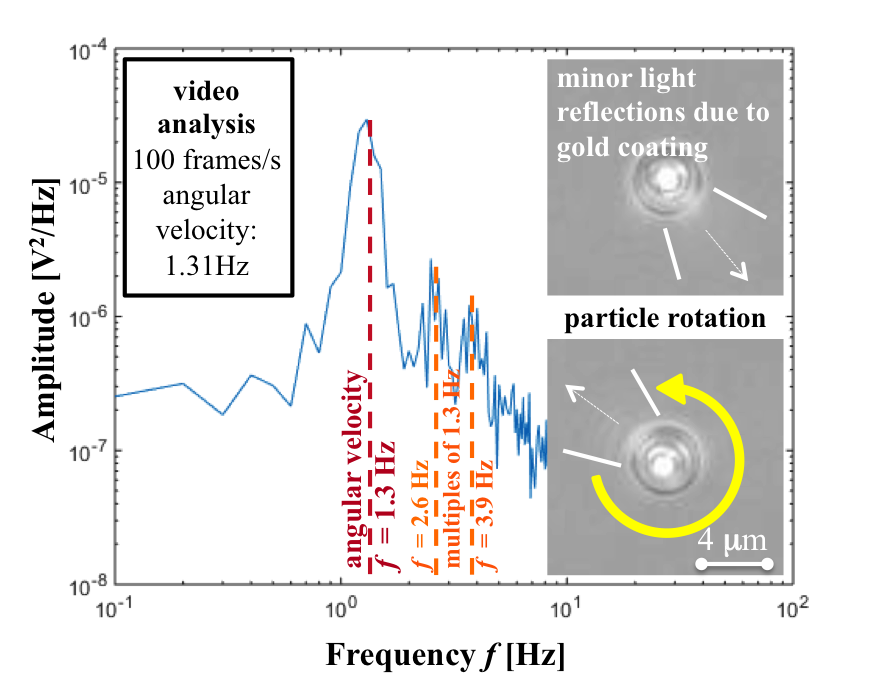
\includegraphics[width=100mm]{\relPath/10_Figures/Fig6.png}
    \caption{Power spectral density and results of the video analysis of a 
      counter-clockwise rotating gold-coated spherical \SI{4.39}{\micro\meter} 
      silica particle at \SI{1090}{\kilo\hertz} and \SI{2.5}{\Vrms} with 
      relative phase shift $\zeta= \sfrac{\pi}{2}$. The 10 times averaged power 
      spectrum of the $y$-signal of the detection unit (QPD) was recorded with a 
      frequency resolution of $\Delta f=\SI{0.1}{\hertz}$ and a sampling rate of 
      \SI{1}{\MS}. A clear peak at \SI{1.3}{\hertz} and two additional peaks at 
      \numlist{2.6; 3.9} \si{\hertz} were observed. The amplitudes of the 
      additional peaks were one order of magnitude smaller as the amplitude of 
      the peak at \SI{1.3}{\hertz}. The peak at \SI{1.3}{\hertz} correlates with 
  the determined rotational rate by the high-speed video analysis at a frame 
  rate of \SI{100}{\fps}.\label{fig:VT-Fig6}}
\end{figure}%
%%%%%%%%%%%%%%%%%%%

\subsection{Rotation of particles where $\normBdLayer \approx 
1$\label{sec:VT-rotationParticles}}

The determinations of the rotational rate with the power spectrum-method opened 
the possibility to measure fast rotations ($>\SI{25}{\hertz}$ (\SI{1500}{\rpm})) 
of particles with a radius $R$ about \SI{1}{\micro\meter}.  For such small 
particles the ratio of the thickness of the viscous boundary layer $\delta$ and 
the particle radius $R$ approaches 1 ($\normBdLayer \approx 1$) in the 
\si{\mega\hertz}-range (\SIrange{1}{10}{\mega\hertz}). The analytical formulas 
become invalid for the case that $\normBdLayer > \sfrac{1}{15}$ \cite{Hahn2016}.  
Particle rotations within the limit $\normBdLayer \approx 1$ were experimentally 
validated by an investigation of silica spheres with a \SI{2.06}{\micro\meter} 
(Microparticles GmbH, Berlin, Germany) diameter resuspended with a 
water/glycerol (70$\%$/30$\%$) mixture.  The viscosity $\mu_f$ of the aqueous 
glycerol solution was \SI{0.06}{\pascal\second} \cite{Jerome1968} with a 
determined density of \SI{1.1}{\gram\per\centi\meter\cubed} (dense knife, DMA 
35N, Anton Paar GmbH, Graz, Austria) and increased the thickness of the viscous 
boundary layer to approximately \SI{1.33}{\micro\meter} at an excitation 
frequency of \SI{1043}{\kilo\hertz} ($\lambda \approx \SI{1.4}{\mm}$). The 
normalized viscous boundary layer is therefore $\normBdLayer \approx 1.30$.

The optical trapping set-up was originally designed to measure the acoustic 
force and pressure amplitudes inside micro-fluidic channels and cavities 
\cite{Lakaemper2015,Lamprecht2016}. The same procedure was used here to measure 
the local acoustic pressure amplitudes inside the fluid chamber of the 
transparent micro-device. An accurate prediction of the acoustic pressure 
amplitudes $A_{X}$ and $A_{Y}$ of the two orthogonal standing waves was 
important to determine the strength of the acoustic VT by observing the 
steady-state rotational rate $\finalOmega$ of rotating particles.

Therefore, the local acoustic pressure amplitudes $A_{X}$ and $A_{Y}$ were 
individually measured in $x$- and $y$-direction by exciting only one transducer 
of the corresponding $x$- or $y$-direction, respectively. We measured the 
acoustic forces in all three dimensions ($x$, $y$, $z$) acting on the 
\SI{2.06}{\micro\meter}-particle inside the optical trapping potential. The 
spatial measurement range was $\pm \SI{0.55}{mm}$ in the $x$- and $y$-direction.  
The point $(\SI{0.21}{\mm}, \SI{0.22}{\mm})$, measured relatively to the middle 
of the fluid chamber, corresponded to the spatial position where a pressure 
nodal line in $x$- and $y$-direction overlapped.

The maximal force amplitudes at \SI{1043}{\kilo\hertz} were 
\SIrange{-96}{+25}{\femto\newton} for the $x$-direction and 
\SIrange{-32}{28}{\femto\newton} for the $y$-direction. The peak-to-peak value 
of the determined forces in $y$-direction was about two times weaker than in 
$x$-direction. This factor of 2 was used to calibrate the piezoelectric 
excitation amplitude to reach equal acoustic pressure amplitudes in both 
excitation directions.

The excitation amplitude $U_{el}$ is proportional with the acoustic pressure 
amplitude $A_{x,y}$ ($U_{el} \propto A_{x,y}$), whereas the acoustic radiation 
force $F_{ac}$ has a quadratic dependency of the acoustic pressure amplitudes 
$A_{x,y}$ ($F_{ac} \propto A_{x,y}^2$) \cite{Barnkob2010}. Therefore, the 
excitation amplitude of the piezoelectric transducer in $y$-direction was 
increased by a factor of $\sqrt{2}$ for all further investigations. The acoustic 
pressure amplitude $p_{a}$ was calculated via
%%%%%%%%%%%%%%%%%%%
\begin{equation}
\label{eq:VT-PressurePredictions}
\begin{split}
p_{a}^{2} &= \frac{F}{\pi\,R^{3}\,\kappa_{0}\,\Phi(f_{1},f_{2})} 
\frac{1}{k\,\sin(2k\,x)}\\
&= \frac{F}{\pi\,R^{3}\,\kappa_{0}\,\Phi(f_{1},f_{2})} 
\frac{\lambda_{\text{p}}}{2\pi\,\sin(x\,\sfrac{4\pi}{\lambda_{\text{p}}})}
\end{split}
\end{equation}
%%%%%%%%%%%%%%%%%%%
where a 1-dimensional standing plane wave is assumed \cite{Settnes2012a}. $F$ is 
the force measured with the optical trap, $\lambda_{\text{p}}$ the wavelength of 
the pressure field, $k = \sfrac{2\pi}{\lambda_{\text{p}}}$ the wavenumber, $R$ 
the radius of the spherical particle, $\kappa_{0}$ the compressibility of the 
fluid, $\Phi(f_{1},f_{2})$ the so-called acoustic contrast factor, and 
$\sin(kx)$ the spatial dependency of the standing wave.  Since the force was 
measured at the force maximum $\sin(2\,kx)$ is set to $\sin(\sfrac{\pi}{2}) = 
1$. In addition, because of the value for the normalized viscous boundary layer 
$\normBdLayer \approx 1$, the corrected dipole factor  
$f_{2}(\tilde{\rho},\normBdLayer)$ of \citeauthor{Settnes2012} 
\cite{Settnes2012} was utilized. With this, the determined acoustic pressure 
amplitude for the standing wave in $x$-direction was \SI{245}{\kilo\pascal} for 
the measured acoustic forces and wavelength if an influence of acoustic 
streaming was neglected. 

After the calibration of the excitation amplitudes and the acoustic pressures of 
both acoustofluidic channels the acoustic VT was quantitatively investigated 
inside the fluid chamber. One \SI{2.06}{\micro\meter} silica particle was 
optically trapped and moved in $x$-direction inside the wave field of two 
orthogonal standing waves, while measuring its power spectrum at specified 
measurements points. The location of one specific pressure nodal line for an one 
dimensional standing wave in $x$- and $y$-direction at \SI{1043}{\kilo\hertz} 
was determined at $x=\SI{0.21}{\mm}$ and $y=\SI{0.22}{\mm}$, respectively. These 
nodal lines formed a local pressure node at their intersection if the acoustic 
excitation was shifted in phase with $\zeta = \sfrac{\pi}{2}$. There, the 
acoustic VT had its maximum value. Therefore, a measurement line in 
$x$-direction was defined between $x=0.20\pm0.55~\si{\milli\meter}$ at constant 
$y=\SI{0.22}{\milli\meter}$.

The particle exerted a counter-clockwise rotation at the local pressure node due 
to the acoustic VT at \SI{1043}{\kilo\hertz} with \SI{10.0}{\Vrms} and 
\SI{14.2}{\Vrms} excitation amplitude in $x$- and $y$-direction, respectively.

The detection of the angular frequency in a recorded power spectrum was not 
trivial for those small and spherical silica particles due to their low 
signal-to-noise ratios. Additionally, the power spectrum was disturbed by added 
frequencies of the acoustic excitation set-up; namely, an additional peak at 
\SI{100}{\hertz} originating from the voltage supply and \SI{170}{\hertz} from 
the amplifier itself.  Therefore, all measurements were repeated with a 
ten-times lower excitation amplitudes in $x$- and $y$-direction to calibrate the 
power spectrum measurements due to unknown influences of the environment and 
attached set-ups. An initialization of particle rotations was not observed at 
these low excitation amplitudes. A peak detection algorithm (implemented in 
MatLab) used the calibration measurement to eliminate disturbances on the 
determined power spectrum of a locally rotating particle due to VT.\@

\Cref{fig:VT-Fig8} depicts the power spectrum of a rotating particle with a clear 
peak at a frequency of \SI{165}{\hertz}. The particle was located at the 
relative location (-0.075, 0.220) \si{\mm} and its rotation was initialized at 
\SI{1043}{\kilo\hertz} with an excitation amplitude of \SI{10.0}{\Vrms} and 
\SI{14.2}{\Vrms} in $x$- and $y$-direction, respectively.  An appearance of 
additional peaks at a multiple of the angular frequency was not monitored by the 
peak-detection algorithm, likely because the amplitude of these peaks was below 
the noise floor. Their signal strength was expected to be one order of 
magnitude smaller (see \cref{fig:VT-Fig5,fig:VT-Fig6}).  The detection 
algorithm had a threshold value of 3 (signal-to-noise ratio) for indicating 
peaks in determined power spectrum.  \cref{fig:VT-Fig8}b depicts the 
corresponding calibration power spectrum of \cref{fig:VT-Fig8}a.

\Cref{fig:VT-Fig10} depicts the peaks detected by the peak-detection algorithm. 
Each point represents a separate rotational rate measurement. Interestingly, the 
strength of the angular frequency peaks was proportional to Brownian noise with 
$\sfrac{1}{f^2}$. These peaks are due to the particle rotations at positions 
within the spatial range of $x=0.21\pm\SI{0.55}{\mm}$ and $y=\SI{0.22}{\mm}$.  
The spatial dependency and formation of these peaks were in correlation with 
\cref{eq:VT-Eq1} and the maximal frequency $f$ of a peak in the power spectrum was 
\SI{229}{\hertz} ($ \finalOmega = \SI{13.8e3}{\rpm} $). The quantitative 
analysis revealed that maximal rotation appeared at $x=\SI{0.16}{\mm}$ (pressure 
node) and the resulting acoustic wavelength in $x$-direction was \SI{1.9}{\mm}.  
A one-dimensional wave in water at $f=\SI{1043}{\kilo\hertz}$ predicts an 
acoustic wavelength of $\lambda = \sfrac{c}{f} \approx \SI{1.4}{\mm}$ (compare 
\cref{fig:VT-Fig4}). The difference in wavelength from \cref{fig:VT-Fig4} 
($\lambda \approx \SI{1.4}{\mm} $) to the fitted value of $\lambda \approx 
\SI{1.9}{\mm} $ may be related to an off-set in orientation of the 
3-dimensional wavenumber $|\vb{k}|^{2} = k^{2}_{x} + k^{2}_{y} + k^{2}_{z}$ in 
the optical trapping set-up. Eigenfrequencies and their acoustic fields are 
influenced by the optical trapping set-up due to the additional interface 
between the acoustofluidic device and the water-immersion objective 
\cite{Lamprecht2016}.  \Cref{fig:VT-Fig4} was observed with a standard 
microscope lens that did not need to have an immersion oil layer on top of the 
device.

%%%%%%%%%%%%%%%%%%%
\begin{figure}
    \centering
    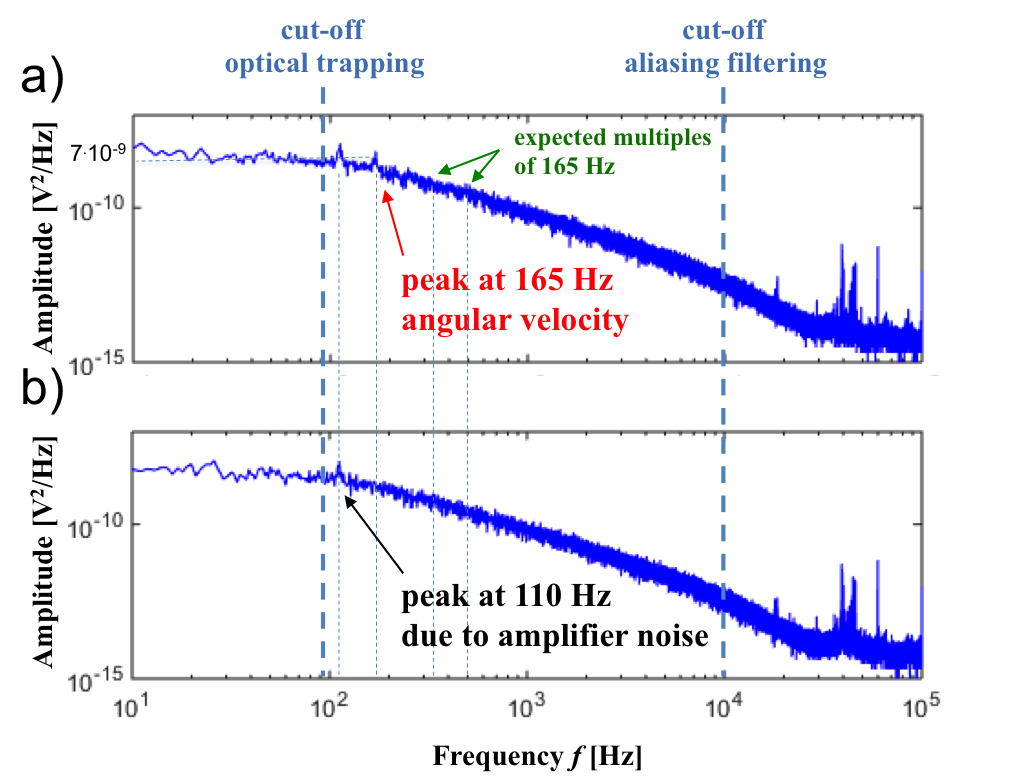
\includegraphics[width=100mm]{\relPath/10_Figures/Fig9.png}
    \caption{a) Measured power spectrum of an optically trapped 
    \SI{2.06}{\micro\meter} particle that rotated counter-clockwise due to the 
    acoustic VT at \SI{1043}{\kilo\hertz} with \SI{10.0}{\Vrms} and 
    \SI{14.2}{\Vrms} excitation amplitude in $x$- and $y$-direction, 
    respectively. The particle was located at (-0.075, 0.220) \si{\mm}. The 
    spectrum of the $x$-signal (QPD) was recorded and 10 times averaged with a 
    frequency resolution of $\Delta f=\SI{1}{\hertz}$ and a sampling rate of 
    \SI{1}{\MS}. A clear signal peak due to particle rotation at 
  \SI{165}{\hertz} was observed with a signal-to-noise ratio of about 5. The 
signal peak at \SI{110}{\hertz} is related to influences of the acoustic 
excitation set-up.\ b) Control measurement of a non-rotating optically trapped 
\SI{2.06}{\micro\meter} particle under acoustic excitation at 
\SI{1043}{\kilo\hertz} with \SI{1}{\Vrms} and \SI{1.42}{\Vrms} excitation 
amplitude in $x$- and $y$-direction, respectively. A particle rotation was not 
initialized at these low excitation amplitudes and these recorded power spectrum 
of non-rotating \si{\micro\meter} particles were used to identify the peaks not 
related to particle rotation power spectrum due to influences of the environment 
and the acoustic excitation set-up. The peak at \SI{110}{\hertz} is related to 
amplifier noise and vanished when the acoustic excitation set-up was turned off 
\cite{Lamprecht2016}.\label{fig:VT-Fig8}}
\end{figure}
%%%%%%%%%%%%%%%%%%%

%%%%%%%%%%%%%%%%%%%
\tikzsetnextfilename{VT_results}
\begin{figure}[tb]
  \centering
  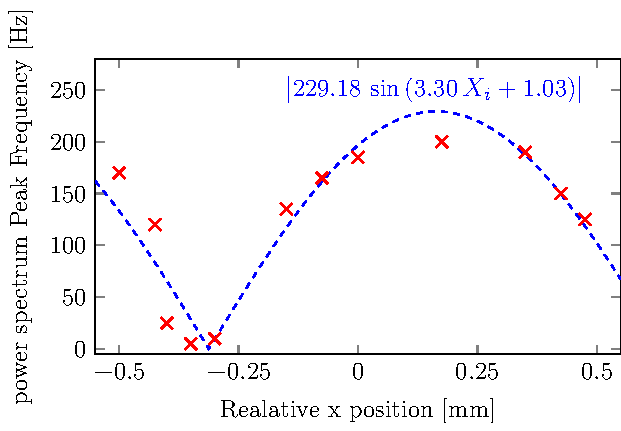
\includegraphics[]{External/VT_results.pdf}
    % \begin{tikzpicture}
    %     \begin{axis}
    %         [scale only axis,
    %         width = 89mm,
    %         height = 5cm,
    %         xtick = {-0.5,-0.25,0,0.25,0.5},
    %         xmin = -0.55, xmax = 0.55,
    %         ymax = 280, ymin = -5,
    %         xlabel = {Realative x position [\si{\mm}]},
    %         ylabel = {power spectrum Peak Frequency [\si{\hertz}]}]

    %         \addplot[red,thick,mark size=4pt,only marks,mark=x] table[x=y, 
    %         y=f,col sep=comma] {\relPath/40_Fitting/datapoints.dat};

    %         \addplot[thick,blue,dashed] table[x=y, y=f,col sep=comma] 
    %         {\relPath/40_Fitting/datapointsFit.dat};

    %         \node[blue,above] at (axis cs: 0.16,229) 
    %         {$\left|229.18\,\sin\left(3.30\,X_{i} + 1.03 \right)\right|$};

    %     \end{axis}
    % \end{tikzpicture}
    \caption{Spatial dependency of frequency peaks (red) due to the acoustic VT 
      from the power spectrum-method. Multiple power spectra of a 
      \SI{2.06}{\micro\meter} silica particle were recorded at specific 
      measurement points in $x$-direction at $x=\SI{0.21}{\mm}\pm\SI{0.5}{\mm}$ 
      and $y=\SI{0.22}{\mm}$. The acoustic field formed two orthogonal standing 
      waves in $x$- and $y$-direction at \SI{1043}{\kilo\hertz} with a relative 
      phase shift of $\zeta =\frac{\pi}{2}$. The determined frequency peaks were 
      fitted to the equation $\left|c_{1}\,\sin(c_2\,X_i + c_3)\right|$ (dashed 
      blue).  The resulting maximal frequency $f$  from the fit was 
      \SI{229}{\hertz} ($ \finalOmega = \SI{13.8e3}{\rpm}$) and the determined 
      acoustic wave in $x$-direction $\lambda_{X}=\sfrac{2\pi}{c_2}$ was 
    \SI{1.90}{\mm}. The pressure nodal point with maximal rotational rate was 
  determined at $x=\SI{0.16}{\mm}$, whereas zero VT was determined at 
$x=\SI{-0.31}{\mm}$ (pressure anti-node).\label{fig:VT-Fig10}}
\end{figure}
%%%%%%%%%%%%%%%%%%%

\section{Conclusion\label{sec:VT-conclusion}}

The combination of an optical trap and a transparent VT device opened the 
possibility to measure the VT independently of the acoustic radiation force. The 
power spectrum analysis provided the quantitative information about the angular 
frequency $\Omega$. Unwanted effects related to close proximities of walls near 
the rotating particle and influences of oscillating micro gas bubbles were 
avoided.  The optically levitated particle ensured a largely unaffected rotation 
due to the acoustic VT.\@ 

Moving the stage of the optical set-up changed the rotation direction of a 
trapped and rotated particle between two neighboring pressure nodes because of 
the acoustic VT \cite{Lamprecht2015} (see the supplemental material for a 
particle rotation in different directions depending on the spatial location 
inside the wave field).  These kinds of experiments were so far unattainable in 
a continuous manner and for unstable acoustic particle positions (positive 
acoustic contrast factor) of zero VT.\@

The validation experiments showed that the detected additional peaks in the 
measured power spectrum are directly related to the rotational rate of the 
particle rotation. The detected signals had peaks at multiples of this peak 
frequency.  However, for transparent silica particles with an almost perfectly 
spherical shape the amplitudes of the multiples were too small to overcome the 
signal-to-noise-ratio. The high-speed video analysis is limited by the camera's 
frame rate. In contrast, the detection bandwidth of the optical trap easily 
spans tens of \si{\kilo\hertz}. As already mentioned, optical trapping has some 
unique advantages to investigate the acoustic VT: 1) Allows to probe almost  any 
spatial position within the acoustofluidic device. 2) Measures rotational 
frequencies up to multiple \si{\kilo\hertz}. 3) Works with conventional, non 
coated, spherical particles. 4) Frequencies are directly visible in the data (no 
need for post processing of video data).

In order to calculate the theoretical rotational rate $\finalOmega$ of the 
particle, the local acoustic pressure amplitude needs to be known in advance.  
Because of that, a local acoustic pressure amplitude analysis was carried out 
before the rotation detection experiments. Depending on the calculation 
approach, different results are obtained for the rotational rate. The analytical 
calculation for the final rotational rate $\finalOmega$ (see \cref{eq:VT-Eq1}) 
\cite{Lamprecht2015, Busse1981, Rudnick1977, Wang1989} with a dynamic fluid viscosity of 
$\mu_{f} = \SI{0.06}{\pascal\second}$ led to rates between 
\SIrange{613}{811}{\hertz} (\SIrange{36.8e3}{48.7e3}{\rpm}). The numerical 
calculations of \citeauthor{Hahn2016} \cite{Hahn2016} yield a final rotational 
rate for a \SI{2.06}{\micro\meter} silica particle with $\normBdLayer=1.30$ of 
\SIrange{208}{277}{\hertz} (\SIrange{12.5e3}{16.6e3}{\rpm}) at room temperature 
(\SI{25}{\celsius}).  The first value for the rotational rate corresponds each 
time to the theoretical wavelength of $\lambda \approx \SI{1.4}{\mm}$ (see 
\cref{fig:VT-Fig4}) and acoustic pressure amplitude $p_{a}\left(\lambda\right) = 
\SI{245}{\kilo\pascal} $; the latter to the measured $\lambda \approx 
\SI{1.9}{\mm}$ (see \cref{fig:VT-Fig10}) and $p_{a}\left(\lambda\right) = 
\SI{282}{\kilo\pascal} $. The disagreement between our experiments and 
\cref{eq:VT-Eq1} is regarding the equilibrium state for the final rotational rate 
$\finalOmega$. The spatial dependency of \cref{eq:VT-Eq1} ($\cos\left(k\,X\right), 
\cos\left( k\,Y \right)$) agrees with our experiments.

In contrast to that, the power spectrum-method estimates the steady-state 
rotational rate $\finalOmega$ to \SI{229}{\hertz} (\SI{13.8e3}{\rpm}). This 
value is very close to the numerically obtained values (about 10$\%$ higher for 
$\lambda \approx \SI{1.4}{\mm}$ or 17$\%$ lower for $\lambda \approx 
\SI{1.9}{\mm}$).  These deviations can be in part explained by a decrease of 
the fluid viscosity due to laser-induced heating (up to \SI{2}{\kelvin}) in 
close proximity of the laser focus \cite{Peterman2003}. Since the measured force 
of our trap scales with $\sqrt{\mu}$ and the viscosity variation around 
\SI{25}{\celsius} is relatively small, the temperature induced measurement 
errors are about 2\%.  This slightly changes the acoustic pressure amplitudes 
with respect to the calibrated pressure of \SI{245}{\kilo\pascal} ($\lambda 
\approx \SI{1.4}{\mm}$) or \SI{282}{\kilo\pascal} ($\lambda \approx 
\SI{1.9}{\mm}$) because the investigated pressure node was located slightly off 
the calibration lines.  Also, the in oil immersed lens of the optical trap 
changes the theoretical (pure) 1-dimensional acoustic field to a 3-dimensional.

The experiment clearly showed that the analytical calculations of 
\citeauthor{Lamprecht2015,Busse1981, Rudnick1977, Wang1989} \cite{Lamprecht2015, Busse1981, 
Rudnick1977, Wang1989}  overestimate the rotational velocities at ratios $\normBdLayer 
\approx 1$. Furthermore, the complexity and spatially varying torques on 
\si{\micro\meter} particles were measured, whereas the simulations are limited 
to the ideal case of plane-standing waves and incompressible particles in an 
infinitely large fluid domain. 

A further application of the acoustic torque analysis with an optical trap could 
be the experimental determination of the influence of the particle density on 
the acoustic VT.\@ Particles with the same density can show different rotational 
directions at a fixed point in the acoustic field, if the ratio $\normBdLayer$ 
changes \cite{Hahn2016}.

Optical torques on double refracting quartz particles is a possible tool to 
directly measure acoustic torques \cite{La2004}. The laser power of such 
modulated optical traps could be used to calibrate acoustic torques on trapped 
particles at equilibriums where the optical torque counteracts the acoustic 
torque. 

% \vspace*{7mm}

% A.L and C.G. contributed equally to this work.



% \cleardoublepage
% \chapter[Discussion \& Outlook]{Discussion and Outlook}\label{ch:discussion}

\section{Discussion}
In this thesis we presented the application of the fast position readout of an 
optically trapped spherical particle to two micro scale acoustofluidics (MSAF) 
phenomena: 1) the transient build up behaviour of acoustic streaming (AS) as 
well as of the acoustic radiation force (ARF); 2) the viscous torque induced 
rotation of spherical particles in a viscous fluid where the viscous boundary 
layer (VBL) thickness is as large as the particle radius itself $\delta \approx 
R$.

The investigations of both phenomena were possible because the laser beam 
causing the trapping potential carries positional information about the 
relative particle position to the laser focal point. In order to extract this 
information from the laser beam, the beam hast to be be collimated again after 
the trapping and focused onto photo detectors. For the resolution of two 
orthogonal directions of the in-plane movement, the photo detector (PD) has to 
be a quadrant photo detector (QPD). For the axial movement a single PD is 
sufficient because only the total intensity onto the PD is needed. However, we 
have two QPDs in our setup.

The physical unit of the QPDs output is \si{\volt}. In order to convert the 
voltage to the unit of \si{\meter}, we took advantage of the linear regime of 
QPDs where a change in measured voltage is proportional to the movement of the 
particle within the trap. In this regime, the optical trap (OT) can also be 
used as force measurement device because it has the same properties as a linear 
mechanical spring for small particle displacements in the order of $0.1\R$. 
The respective start and end point of this regime is dependent on a multitude 
of parameters. But, movements of less than \SI{100}{\nm} are still linear for 
our OT setup. The voltage-conversion factor as well as the stiffness of the OT 
can be derived from the single-sided frequency spectrum of the trapped 
particle. The particles in the fluid suspended were so lightweight and small 
that they showed visible Brownian motion. Brownian motion is a random process 
with the property that over a long time period the particle will be back at its 
initial position. Also, while being trapped the particle showed Brownian 
motion. The frequency content of a trapped particle in any spatial direction 
follows the curve of a low-pass filter. With the amplitude at zero frequency 
$A_{0}$ and the cutoff frequency $f_{\MR{c}}$ where 
$A\vert_{f=f_{\MR{c}}}=\sfrac{A_{0}}{2}$ it was possible to calculate the 
voltage-meter conversion factor as well as the stiffness for each spatial 
direction independently.

Besides the size of the trapped particle the conversion factor is dependent on 
the viscosity of the surrounding fluid. Exact knowledge of the viscosity is a 
requirement for quantitatively precise measurements. The viscosity of the fluid 
is in general a function of its temperature. While the ambient temperature was 
straightforward to measure, the measurement of the temperature within a MSAF 
device or at the focal point of the trapping laser was cumbersome. Although the 
intensity of our laser exceeds the sun's intensity by orders of magnitudes, we 
showed in \cref{sec:TO-temperature} that for our setup the laser induced 
temperature change and therefore the temperature induced viscosity change is 
negligible for all our experiments. However, this is not true for every OT 
because the temperature change does not only depend on the laser power itself 
but even more on the laser wavelength-fluid combination, and therefore the 
absorption at a specific wavelength.

To investigate the first MSAF phenomena, we developed a new measurement method 
in \cref{ch:timeconstant} to visualize the transient build up of the ARF and AS 
and then studied in \cref{ch:pulsing} the effects of a pulsed excitation on the 
respective build up times. Key for those experiments was, that the ARF and AS 
induced particle displacement were along orthogonal spatial direction. 
Moreover, the ARF displacement was along one of the axes of the in-plane QPD 
and the AS displacement was along the axial direction on another QPD. Hence, 
the measured displacement data is also separated and cross-talk free. We 
validated the orthogonality of the ARF and the drag force from AS by steady 
state force measurements with two different sized particles where all 
experimental parameters besides the particle radius were kept the same. The 
drag force from AS scales with the particle radius, $\FAS\propto R$ and the ARF 
with the volume of the particle, $\FARF\propto R^{3}$. The ratio of the 
measured forces along same directions but of different particle sizes showed 
the same scaling laws. 

However, without modifications on the OT we were not able to measure any of 
those effects because the timeconstant of the OT $\tOT$ is much larger than the 
theoretical build up time of the ARF. In fact, for our set of experimental 
parameters and our device configuration $\tOT \approx \tas \gg \tarf$ with 
$\tas = \SI{1.59}{\ms}$ and $\tarf = \SI{1.4}{\us}$, respectively. We reduced 
$\tOT$ effectively to zero by reducing the laser power to almost zero such that 
there was no effective trapping by the OT. The laser cannot be switched off 
completely because the beam is the cause for the measured intensity at any of 
the QPDs.

Because of the laser power reduction, we also needed to install an optical 
shutter right before the QPDs. The laser intensity is too high for the photo 
detectors. In normal trapping mode a set of filters reduces the intensity to 
less than 0.01\% of the incoming intensity. The optical filter is actuated to 
be almost completely closed such that it acts as intensity filter if the laser 
power is high (trapping) and opens as soon as the laser power is reduced for 
the measurement itself.

The laser power change occured almost instantaneously but the shutter had an 
opening time of less than \SI{15}{\ms}. To ensure undisturbed data we waited 
\SI{25}{\ms} before starting the acoustic excitation. During this time the 
particle will start to sediment due to gravity because it was not trapped 
stably anymore. However, this movement was only $\approx 0.05\,R$ along the 
direction of the laser beam and, hence, did not hinder the measurement; the 
in-plane movement was zero because no forces besides gravity are acting on the 
particle.

The (pulsed) acoustic excitation was then switched on for only \SI{30}{\ms} 
because a longer excitation would lead to such large displacements -- primarily 
along the ARF direction -- that the same particle could not be re-trapped by 
the OT. For our studies we were not interested in the actual displacements but 
in the time it takes until the movement along any direction starts. For actual 
displacement magnitudes one would need to retrieve the voltage-meter conversion 
factor but for that the particle needs to be trapped. Hence, only the voltage 
at the QPDs can be investigated.

Because the particle is free-floating and, therefore, uncontrolled in its 
location for the first \SI{25}{\ms} we repeated the measurement multiple times 
per location and averaged the measured data. To further subtract the gravity 
induced movement from the data we perform the same amount of measurements with 
no acoustics at all and then subtract the averaged \emph{no-acoustic} data from 
the \emph{acoustics} data.

The data for both types of experiments (non-pulsed and pulsed) showed that the 
ARF induced displacement starts immediately whereas the AS induced displacement 
takes significantly longer. The measured time offset between ARF and AS is an 
explanation why in experiments~\cname{Hoyos2013} and~\cname{Castro2016} a 
pulsed acoustic excitation suppressed the build up of AS whereas numerical 
investigations~\cname{Muller2015} with an ideal fluid cavity revealed a much 
smaller offset which did not suppress streaming. Although the data had the unit 
of \si{\volt} and not \si{\meter}, the slope of the AS and ARF induced 
displacement was showing that the acceleration after the build up by any of two 
effects occurs fast and then transitions into constant velocity (linear slope). 
A constant velocity implies a constant force acting on the particle.
% It is a valid statement because the measured voltage (within the linear regime 
% of the QPDs) is the displacement divided by the voltage-meter conversion 
% factor. The slope of the voltage-over-time data equals the slope of the 
% displacement which is in turn the velocity of the particle.

Additionally, the pulsed excitation measurements revealed that a pulsed 
excitation leads to a greater reduction in terms of the final displacement at 
the end of the measurement on the AS than it did on the ARF. We measured this 
observation for all pulsing frequencies. The ARF and AS are linearly dependent 
on the acoustic energy density within the fluid cavity. All our data also 
showed this relation but with a steeper slope for AS than the ARF. The pulsed 
excitation results help to further explain the experimentally shown suppression 
of AS~\cite{Hoyos2013,Castro2016}. However, with our measurement protocol we 
can only measure for the first \SI{30}{\ms} of the acoustic excitation, but any 
MSAF application is operated continuously where all fields have developed 
fully.
% At the moment, we cannot measure these effects during steady-state.


Compared to the first phenomena, no setup modifications at the OT were 
necessary for the second MSAF phenomena: the rotational speed measurement of a 
spherical particle driven by the viscous torque (\cref{ch:viscoustorque}). The 
two main requirements for the generation of a viscous torque that is 
sufficiently large to initiate a particle rotation are: 1) the formation of a 
VBL $\delta$ around the particle; 2) a two dimensional orthogonal acoustic 
excitation with phase difference such that the acoustic pressure at the 
particle surface has a continuous phase change in circumferential direction.

The second requirement was straightforward to accomplish by the use of a 
quadratic fluid cavity where the excitation is applied to the system from two 
orthogonal directions. The phase difference of the two excitation signals could 
easily be realized with most dual channel function generators. The viscosity 
increase of the fluid and therefore the larger VBL around the particle can be 
created by a glycerol water mixture (3:7 for our experiments). A greater 
viscosity increase was not possible, because glycerol has the side effect that 
it also increases the refractive index of the mixture. For stable trapping the 
refractive index of the particle must be larger than of the surrounding medium. 
For equal refractive indices the particle is \emph{invisible} for the laser 
beam because no path change of the light occurs at the particle-fluid 
interface. A greater index of refraction of the particle than the fluid index 
leads to repulsion of the particle from the laser focal point.

Our measurement utilized the property that a distinct amplitude peak appears at 
the rotational frequency of the particle in the one sided power spectrum of the 
trapped rotating particle. We validated this finding with deformed and partial 
gold coated particles where the rotation was also visible optically. By having 
a highspeed camera mounted to the OT and choosing the excitation parameters 
such that the viscous torque induced rotation is clearly visible, the 
rotational speed measurement from the power specturm could be validated by the 
analysis of the single frames from the video. The deformed particles did not 
rotate with a single constant velocity because of their non-spherical shape. 
Therefore, multiple additional peaks were also visible in the power spectrum.  
However, the partially gold coated particles with perfect spherical shape 
showed a single peak that matched the rotational speed from the optical 
analysis.

With a validated method for measuring the rotational speed of a spherical 
particle we investigated the situation where the particle radius is as big as 
the VBL thickness itself ($R\approx\delta$). In the regime where $\delta > 
\sfrac{R}{15}$ a numerical study by \cname{Hahn2016} predicted the final 
terminal rotational velocity order of magnitudes lower than a theoretical 
investigation by \cname{Lamprecht2015}. Note here, that~\cname{Lamprecht2015} 
restricted their calculations to the assumption that $R\gg\delta$. Our 
measurements of rotations up to \SI{13700}{\rpm} confirmed the results from 
\cname{Hahn2016} and also confirmed the limited validity of the theoretical 
formula of \cname{Lamprecht2015} in the regime where $R\approx\delta$.

\section{Outlook}

The OT is a great tool for measuring acoustic effects on micro-scale particles 
suspended in a fluid. The four main advantages are: 1) measurements on a single 
particles; 2) high spatial precision and repeatability of the measurement 
locations; 3) high temporal resolution of particle position; d) high 
sensitivity to surroundings. The last point is also by far the biggest 
disadvantage. For all our experiments we were very cautious about us being in 
the lab during the measurements and any other disturbances, like fast and 
careless opening/closing of the door or like constructions works in the 
neighboring lab. In any case, the combination of the optical trap as 
characterization/measurement device for the acoustical trap offers many 
possible future research contributions. In the following we want to categorize 
our suggestions in three sections: a) deeper theoretical understanding of the 
OT; b) future experiments with our setup where no big modifications are needed; 
c) more general ideas which would need larger modifications to our setup.

\subsection{Optical Trap Calibration}

In this thesis we did not explain the calibration protocol for our OT. As 
before, interested readers are pointed to the thesis of \cname{Lamprecht2017} 
(Section 3.2.4) where our calibration process is explained in great detail. The 
basic procedure is to fit a low-pass filter to the frequency content of a 
trapped particle. This fitting is based on two parameters: the amplitude 
$A_{0}$ at zero frequency and the cut-off frequency $f_{\MR{c}}$. With those 
two parameters the stiffness $\kappa_{i}\propto f_{\MR{c}}$ and the 
voltage-meter conversion factor $r_{i}\propto \sfrac{1}{(f_{\MR{c}}\sqrt{A_{0}} 
)}$ can be calculated for all three spatial directions separately. The total 
force is then simply the product of the measured voltage times the two factors 
and, hence, \begin{equation}
  \force_{i,\MR{measured}}\propto \kappa_{i}\,r_{i}\propto 
  \sfrac{1}{\sqrt{A_{0}}}.
\end{equation}
Interestingly, the measured force is only proportional to one of those fitting 
parameters $A_{0}$. The fit itself, especially, the parameter $A_{0}$ depends 
highly on the beginning of the data range used for the fit. From experience we 
used for our OT calibration the frequency spectrum data ranging from 
\SI{20}{\hertz} up to \SI{6}{\kilo\hertz} for the $\ex$ and $\ey$ direction and 
\SI{10}{\hertz} to \SI{2}{\kilo\hertz} for $\ez$. The $\ez$ direction has a 
smaller and lower range because it is known that OTs are in general weaker 
along the beam axis and, hence, the respective cut-off frequency is also lower.  
Therefore, an investigation regarding the fitting interval will help increase 
the absolute precision of OTs.

However, the error introduced by a false data range is \emph{just} a false 
scaling of the forces. Measurements that use the same fitting procedure can 
still be compared because all measurements might share the same scaling error. 
Up to our knowledge we are not aware of any publication that discusses (and 
resolves) this small but important detail for the power spectrum OT 
calibration.

\subsection{Future Research with our Optical Trapping Setup}

Although we investigated two MSAF phenomena with our OT setup, there are many 
more open questions and interesting projects. We select three projects which we 
think are of great interest for the MSAF community and also achievable without 
any modifications to our present OT setup.

The first is a variation of \cref{ch:timeconstant,ch:pulsing}. In a first step 
we were able to measure the build up of the two effects, but only for the first 
120'000 excitation periods ($\approx \SI{30}{\ms}$). Although we could show 
that AS is significantly slower in its build up than the ARF, we could not 
investigate the steady-state behavior of a pulsed excitation. Therefore, we 
suggest to measure the steady-state forces exerted on a single particle for 
various pulse frequencies settings and compare the forces to a non-pulsed 
measurement. To reduce uncertainties between different settings and increase 
data comparability, one should create a measurement protocol where all data is 
measured with one device initialization.

The second possible field of interest is also investigating the ARF and AS.  
However this time, one would be investigating the scaling laws of AS and the 
ARF. From theory we know that they scale $\propto R$ and $\propto R^{3}$ for a 
spherical particle, respectively. The total acoustic force 
$\forcevector^{\MR{ac}}$ is understood to contain a linear part from AS and a 
cubic part due to the ARF
\begin{equation}
  \forcevector^{\MR{ac}}\left( R \right) = \vb{C}^{\MR{AS}}\,R + 
  \vb{C}^{\MR{rad}}\,R^{3}.
\end{equation}
From force measurements of two different sized particles with the same 
experimental condition it is possible to extract the constants 
$\vb{C}^{\MR{AS}}$ and $\vb{C}^{\MR{rad}}$. Therefore one could image the pure 
fields that are creating the ARF and also that are due to AS. In order to 
validate the assumed composition of the total acoustic force on a particle 
holds, a third measurement with another particle size is needed. Based on the 
constants $\vb{C}^{\MR{AS}}$ and $\vb{C}^{\MR{rad}}$ one is able to predict the 
force field in all three dimensions for the third particle size $R_{3}$
\begin{equation}
  \forcevector^{\MR{ac}}\left( R_{3} \right) = \vb{C}^{\MR{AS}}\,R_{3} + 
  \vb{C}^{\MR{rad}}\,R^{3}_{3}.
\end{equation}
The main challenge for this study is to ensure the same pressure amplitude 
inside the cavity for the three different particle sizes.

The third and last potential study we want to discuss here is a controversy 
about the ARF for heavy particles in viscous fluids. \cname{Baasch2019} showed 
numerically that the contributions of microstreaming around heavy particles in 
a viscous fluid are of such significance that they could lead to a 
force-inversion. Their findings strengthen the theory of 
\cname{Doinikov1994Rigid} which also predicts this force inversion whereas the 
theory of \cname{Settnes2012} does not. With the measurement of the rotational 
speed in a glycerol-water mixture we could already show that the OT can operate 
within viscous fluid. Besides being heavy the other main requirement is to be 
trappable for the OT setup. Additionally, those particles should have the same 
optical absorption as the surrounding fluid because otherwise the laser induced 
heating might be too high such that the changes in viscosity are not negligible 
anymore.

\subsection{Future Optical Trap Research for MSAF}

In the final part of this thesis we will motivate three possible studies that 
are not applicable to our specific OT setup. For the first one, the main 
limitation is not directly our OT but the devices we use. The main requirement 
for our devices is that they are transparent from top to bottom for our laser 
light as well as being wide enough to accommodate the converging cone of the 
laser beam. Therefore, we cannot measure close to walls because the silicon 
walls are non-transparent for our laser wavelength and hinder the laser beam 
and, hence, would violate the assumption of a symmetrical trapping potential 
which is the basis for the trap calibration. Acoustic wall effects are an 
interesting phenomena that are important for narrow channels and could lead to 
further applications. Devices where also the channel side walls are made out of 
glass (all-glass devices) might be an interesting opportunity for studying 
these effects. However, one would need to investigate the refractive index of 
the fluid and the specific glass carefully.

For our investigated applications this is not a problem because the two 
interfaces of the top cover glass with the immersion oil layer and the fluid 
inside the cavity are parallel. Therefore, the beam passes this interface 
without a change in direction. However, in an all-glass device which would be 
used for measuring close to the channel wall some parts of the laser beam will 
be going through the channel wall. For different refractive indices of the 
fluid and the glass this will lead to a deflection of the laser which in turn 
will violate the assumption of a symmetric optical potential. The magnitude of 
the violation is proportional to the index difference. For matching indices of 
the device material and the fluid no deflection at any of those interfaces 
occurs.

Secondly, with an OT consisting of two lasers where one is creating the optical 
potential for trapping and the other is the light source for the position 
detection at the QPDs one is able to re-perform the build up experiments. 
Besides a validation of our results with another setup and device, one would 
also eliminate the lead time before the acoustic excitation starts. This lead 
time was necessary in our case because we have a single beam OT and needed to 
open the optical shutter before we could start the acoustic excitation.

Lastly, our device is a bulk acoustic wave (BAW) device where a standing 
pressure waves is formed in the bulk of the fluid. The other major kind of 
devices are surface acoustic wave (SAW) devices. In those devices opposing 
traveling waves at the coverplate-fluid interface create a standing pressure 
field inside the fluid that can also manipulate objects. Up to our knowledge no 
direct force measurement were performed with SAW devices so far.


% \appendix
% \begin{appendix}
% %\iffalse %Beginn langer Kommentar
\chapter[Appendix]{Supplemental to Chapter 5\label{ch:app-pulsing}}

% \end{appendix}
% \cleardoublepage

% \renewcommand{\bibname}{References} %Rename chapter to References
\addcontentsline{toc}{chapter}{References} %add references to Outline
% \bibliographystyle{siam}
% \bibliography{All}
\printbibliography


\setlength{\parindent}{0mm} %Abschnitt-Einzug auf 0 setzen
\renewcommand{\\}{\newline} %damit wird wieder \\ \\ möglich für doppelte Zeilenabstände


% \chapter*{List of Publications}
\markboth{List of Publications}{List of Publications}                     % heading
\addcontentsline{toc}{chapter}{List of Publications}          % list in table 


\makeatletter
\DeclareCiteCommand{\fullcite}
  {\defcounter{maxnames}{\blx@maxbibnames}%
    \usebibmacro{prenote}}
  {\usedriver
     {\DeclareNameAlias{sortname}{default}}
     {\thefield{entrytype}}}
  {\multicitedelim}
  {\usebibmacro{postnote}}
\DeclareCiteCommand{\footfullcite}[\mkbibfootnote]
  {\defcounter{maxnames}{\blx@maxbibnames}%
    \usebibmacro{prenote}}
  {\usedriver
     {\DeclareNameAlias{sortname}{default}}
     {\thefield{entrytype}}}
  {\multicitedelim}
  {\usebibmacro{postnote}}
\makeatother

%as first author}
\section*{Publications in Peer-Reviewed Scientific Journals}
\begin{itemize}
  \item \fullcite{Lamprecht2021}\footnote{A.L. and C.G. shared first author}
  \item \fullcite{Goering2021}
  \item \fullcite{Goering2022}
  \item \fullcite{Fankhauser2022}\footnote{J.F. and C.G. shared first author}
\end{itemize}


\section*{Oral Presentations at International Conferences}
C. Goering, A. Lamprecht, I.A.T. Schaap, and J. Dual.  \emph{"Direct 
Measurement of Small Spherical Particle Rotation driven by the Acoustic Viscous 
Torque"} Acoustics Virtually Everywhere, 07-11 December 2020, Virtual 
Conference.\\
  \\
C. Goering and J. Dual.\emph{"Measuring the temporal difference in build up 
between the acoustic radiation force and acoustic streaming with an optical 
tweezer."} Acoustofluidics, 26-27 August 2021, Virtual Conference.\\

% \thispagestyle{empty}

\makeatletter
\newcommand\tabfill[1]{%
  \dimen@\linewidth
  \advance\dimen@\@totalleftmargin
  \advance\dimen@-\dimen\@curtab
  \parbox[t]\dimen@{#1\ifhmode\strut\fi}%
}
\makeatother

\begin{floatingfigure}{4.5cm} %Abstand vom rechten Rand (formerly 3.5)
\centerline{ 
\includegraphics[trim={50mm 30mm 50mm 30mm}, clip, width=35mm]{SECTION/Portrait.png}} 
% \label{portrait}
\end{floatingfigure}

\noindent\textbf{ \\ \underline{Christoph} Ludwig Georg Ananda Goering} \\
\begin{flushleft}
\noindent  Born on 17$^\mathrm{th}$ of August 1991 in Augsburg, Germany \\
\end{flushleft}

\vspace{2.8cm} \noindent
\textbf{Education}                                        \\
\vspace{-0.5cm} \noindent


\begin{tabbing}
  \hspace{25mm} \=   \kill


2018--2022 \> \tabfill{PhD student in Prof. J. Dual's group, Institute of 
Mechanical Systems, Swiss Federal Institute of Technology (ETH) Zurich, 
Switzerland}\\
2015--2017 \> \tabfill{M.Sc. in mechanical engineering at the Technical 
University of Munich (TUM), Germany.}\\
2011--2014 \> \tabfill{B.Eng. in \emph{Maschinenbau -- Konstruktion und 
Entwicklung} at Dualen Hochschule Baden-Württemberg (DHBW), Ravensburg, 
Germany.}\\
2002--2011 \> \tabfill{Gymnasium bei St. Stephan, Augsburg; graduation with the 
German Abitur.}\\
\end{tabbing}

\vspace{-0.5cm} \noindent
\textbf{Professional experience}\\
\vspace{-0.8cm} \noindent
\begin{tabbing}
  \hspace{25mm} \=   \kill
  2018--2022 \> \tabfill{PhD Student at ETH, Zurich, Switzerland.}\\
  2015--2017 \> \tabfill{Werksstudent at BMW AG, Munich, Germany.}\\
  2011--2014 \> \tabfill{Dualer Student at Zeppelin Systems GmbH, 
  Friedrichshafen, Germany.}\\
  2011--2017 \> \tabfill{Auxiliary staff at MABRIS, Augsburg, Germany.}\\
\end{tabbing}

\vspace{-0.5cm} \noindent
\textbf{Extra curricular activities}\\
\vspace{-0.8cm} \noindent
\begin{tabbing}
  \hspace{25mm} \=   \kill
  2012--2015 \> \tabfill{Member of Global Formula Racing (GFR); winner of 
  multiple events overall in the Formula Student.}\\
  1991-- \> \tabfill{Being outdoors.}\\

\end{tabbing}


\end{document}
